\documentclass[twoside]{book}

% Packages required by doxygen
\usepackage{calc}
\usepackage{doxygen}
\usepackage{graphicx}
\usepackage[utf8]{inputenc}
\usepackage{makeidx}
\usepackage{multicol}
\usepackage{multirow}
\usepackage{textcomp}
\usepackage[table]{xcolor}

% Font selection
\usepackage[T1]{fontenc}
\usepackage{mathptmx}
\usepackage[scaled=.90]{helvet}
\usepackage{courier}
\usepackage{amssymb}
\usepackage{sectsty}
\renewcommand{\familydefault}{\sfdefault}
\allsectionsfont{%
  \fontseries{bc}\selectfont%
  \color{darkgray}%
}
\renewcommand{\DoxyLabelFont}{%
  \fontseries{bc}\selectfont%
  \color{darkgray}%
}

% Page & text layout
\usepackage{geometry}
\geometry{%
  a4paper,%
  top=2.5cm,%
  bottom=2.5cm,%
  left=2.5cm,%
  right=2.5cm%
}
\tolerance=750
\hfuzz=15pt
\hbadness=750
\setlength{\emergencystretch}{15pt}
\setlength{\parindent}{0cm}
\setlength{\parskip}{0.2cm}
\makeatletter
\renewcommand{\paragraph}{%
  \@startsection{paragraph}{4}{0ex}{-1.0ex}{1.0ex}{%
    \normalfont\normalsize\bfseries\SS@parafont%
  }%
}
\renewcommand{\subparagraph}{%
  \@startsection{subparagraph}{5}{0ex}{-1.0ex}{1.0ex}{%
    \normalfont\normalsize\bfseries\SS@subparafont%
  }%
}
\makeatother

% Headers & footers
\usepackage{fancyhdr}
\pagestyle{fancyplain}
\fancyhead[LE]{\fancyplain{}{\bfseries\thepage}}
\fancyhead[CE]{\fancyplain{}{}}
\fancyhead[RE]{\fancyplain{}{\bfseries\leftmark}}
\fancyhead[LO]{\fancyplain{}{\bfseries\rightmark}}
\fancyhead[CO]{\fancyplain{}{}}
\fancyhead[RO]{\fancyplain{}{\bfseries\thepage}}
\fancyfoot[LE]{\fancyplain{}{}}
\fancyfoot[CE]{\fancyplain{}{}}
\fancyfoot[RE]{\fancyplain{}{\bfseries\scriptsize Generated on Wed Oct 15 2014 10\-:54\-:02 for K\-I\-S\-S\-C\-P\-P by Doxygen }}
\fancyfoot[LO]{\fancyplain{}{\bfseries\scriptsize Generated on Wed Oct 15 2014 10\-:54\-:02 for K\-I\-S\-S\-C\-P\-P by Doxygen }}
\fancyfoot[CO]{\fancyplain{}{}}
\fancyfoot[RO]{\fancyplain{}{}}
\renewcommand{\footrulewidth}{0.4pt}
\renewcommand{\chaptermark}[1]{%
  \markboth{#1}{}%
}
\renewcommand{\sectionmark}[1]{%
  \markright{\thesection\ #1}%
}

% Indices & bibliography
\usepackage{natbib}
\usepackage[titles]{tocloft}
\setcounter{tocdepth}{3}
\setcounter{secnumdepth}{5}
\makeindex

% Hyperlinks (required, but should be loaded last)
\usepackage{ifpdf}
\ifpdf
  \usepackage[pdftex,pagebackref=true]{hyperref}
\else
  \usepackage[ps2pdf,pagebackref=true]{hyperref}
\fi
\hypersetup{%
  colorlinks=true,%
  linkcolor=blue,%
  citecolor=blue,%
  unicode%
}

% Custom commands
\newcommand{\clearemptydoublepage}{%
  \newpage{\pagestyle{empty}\cleardoublepage}%
}


%===== C O N T E N T S =====

\begin{document}

% Titlepage & ToC
\hypersetup{pageanchor=false}
\pagenumbering{roman}
\begin{titlepage}
\vspace*{7cm}
\begin{center}%
{\Large K\-I\-S\-S\-C\-P\-P }\\
\vspace*{1cm}
{\large Generated by Doxygen 1.8.6}\\
\vspace*{0.5cm}
{\small Wed Oct 15 2014 10:54:02}\\
\end{center}
\end{titlepage}
\clearemptydoublepage
\tableofcontents
\clearemptydoublepage
\pagenumbering{arabic}
\hypersetup{pageanchor=true}

%--- Begin generated contents ---
\chapter{Keep It Simple Stupid -\/ C Plus Plus}
\label{index}\hypertarget{index}{}K\-I\-S\-S\-C\-P\-P is a library containing classes, templates and supporting functions to facilitate rapid application development of C++ server side applications. It is in it's part, heavily dependent upon the \href{http://boost.org}{\tt C++ Boost libraries}.


\begin{DoxyItemize}
\item \href{the_basic_problem.md}{\tt The Basic Problem}
\item \href{md_inter_process_communication.html}{\tt Inter Process Communication}
\item \href{md_mandate.html}{\tt Contribution Mandate}
\item \href{md_motivation.html}{\tt Motivation}
\item \href{md_example_echo.html}{\tt Example\-: kc\-\_\-echo} 
\end{DoxyItemize}
\chapter{Keep It Simple Stupid -\/ C Plus Plus}
\label{md__r_e_a_d_m_e}
\hypertarget{md__r_e_a_d_m_e}{}
K\-I\-S\-S\-C\-P\-P is a library containing classes, templates and supporting functions to facilitate rapid application development of C++ server side applications. It is in it's part, heavily dependent upon the \href{http://boost.org}{\tt C++ Boost libraries}.

For more information, please refer to the \href{http://thelastcylon.github.io/kisscpp/index.html}{\tt online documentation}. 
\chapter{Configuration and configuration files.}
\label{md_configuration}
\hypertarget{md_configuration}{}
\subsection*{Format}

After much investigation and debate, J\-S\-O\-N was yet again selected as the preferred format. In the case of configuration files, we found that I\-N\-I format lacks the ability for nested records and X\-M\-L quickly becomes an unreadable mess. The only down side we have identified with the use of J\-S\-O\-N as a configuration file format, was it's lack of native support for comments. This is a shortcoming we are more than willing to live with. If you need comments in your configuration files, you actually need way more than just a configuration file.

\subsection*{Reserved identifiers}

The following are reserved identifiers, for use in configuration files\-: Note\-: The prefix of {\bfseries kcc} is shorthand for (K)iss(\-C)pp (C)onfiguration.

\begin{TabularC}{2}
\hline
\rowcolor{lightgray}{\bf {\bfseries Identifier} }&{\bf {\bfseries Description}  }\\\cline{1-2}
kcc-\/server.\-address &the hostname or ip address of the server. \\\cline{1-2}
kcc-\/server.\-port &the port of the server. \\\cline{1-2}
kcc-\/stats.\-gather-\/period &Seconds between gathering statistics for historic purposes. \\\cline{1-2}
kcc-\/stats.\-history-\/length &Number of historic stats gatherings to keep. \\\cline{1-2}
kcc-\/log-\/level.\-type &The default type limitation on logs. \\\cline{1-2}
kcc-\/log-\/level.\-severity &The default severity limitation on logs. \\\cline{1-2}
kcc-\/white-\/list &A root node containing data regarding white list communications. More detail available {\bfseries T\-O\-D\-O\-: Add link to more detail} \\\cline{1-2}
\end{TabularC}
\subsection*{Configuration file naming standard}

K\-I\-S\-S\-C\-P\-P applications will have configuration files named as follows\-:


\begin{DoxyCode}
<application-\textcolor{keywordtype}{id}>.<application-instance-\textcolor{keywordtype}{id} or \textcolor{stringliteral}{"common"}>.kcppcfg
\end{DoxyCode}


i.\-e. An application with the id \char`\"{}foo\char`\"{}, being executed with an instance identifier of \char`\"{}bar\char`\"{} will look for a configuration file named\-:


\begin{DoxyCode}
foo.bar.kcppcfg
\end{DoxyCode}


This file must contain configuration data that is specific to the {\bfseries foo} application running as instance {\bfseries bar}.

There is however, a mechanism for allowing shared configuration to exist in a single file. This is known as the common-\/configuration file. This file will have the instance id portion of the file name, replaced by the string \char`\"{}common\char`\"{}.

i.\-e. An application with the id {\bfseries foo}, being executed with an instance identifier of {\bfseries bar} will look for shared configuration details in a file named.


\begin{DoxyCode}
foo.common.kcppcfg
\end{DoxyCode}


\subsection*{Configuration file location}

Due to the fact that K\-I\-S\-S\-C\-P\-P is a library meant for large systems consisting of interdependent processes, we did have to standardize on most aspects of the configuration files. The control we can give you, is based around a holistic approach, and the fact that the developer is not the only one that needs to be considered here. System administrators and support personnel also need to have a sane standard to work with.

As such, the following decision were made\-:


\begin{DoxyEnumerate}
\item Only the root path for configuration files, will be under user control. i.\-e. You can specify nothing more than the path under which K\-I\-S\-S\-C\-P\-P will search for the following\-:
\begin{DoxyItemize}
\item A sub-\/directory with a name matching the application-\/id.
\item Files contained in that sub-\/directory, that match the file naming standard discussed above.
\end{DoxyItemize}
\item A mechanism for environment separation will be available. i.\-e. You have the ability to keep environment specific files separated from each other. This mechanism is provided through the {\bfseries K\-C\-P\-P\-\_\-\-E\-X\-E\-C\-\_\-\-E\-N\-V} environment variable
\end{DoxyEnumerate}

The configuration file path, is constructed in one of three ways\-:


\begin{DoxyItemize}
\item Where {\bfseries K\-C\-P\-P\-\_\-\-C\-F\-G\-\_\-\-R\-O\-O\-T} and {\bfseries K\-C\-P\-P\-\_\-\-E\-X\-E\-C\-\_\-\-E\-N\-V} are used\-: \$\-K\-C\-P\-P\-\_\-\-C\-F\-G\-\_\-\-R\-O\-O\-T/$<$application-\/id$>$/\$\-K\-C\-P\-P\-\_\-\-E\-X\-E\-C\-\_\-\-E\-N\-V/$<$application-\/configuration-\/file-\/name$>$
\item Where only {\bfseries K\-C\-P\-P\-\_\-\-C\-F\-G\-\_\-\-R\-O\-O\-T} is used\-: \$\-K\-C\-P\-P\-\_\-\-C\-F\-G\-\_\-\-R\-O\-O\-T/$<$application-\/id$>$/$<$application-\/configuration-\/file-\/name$>$
\item Developers can override any setting of {\bfseries K\-C\-P\-P\-\_\-\-C\-F\-G\-\_\-\-R\-O\-O\-T} by specifying the path at the time of instantiating the Server class.
\end{DoxyItemize}

That means, when you have a K\-I\-S\-S\-C\-P\-P application with the name {\bfseries foo} and you start instance {\bfseries bar} of it, while having {\bfseries K\-C\-P\-P\-\_\-\-C\-F\-G\-\_\-\-R\-O\-O\-T} set to {\bfseries /put/configurations/here}

Your application will look in\-:
\begin{DoxyItemize}
\item /put/configurations/here/foo
\item for a files named
\begin{DoxyItemize}
\item foo.\-common.\-kcppcfg and
\item foo.\-bar.\-kcppcfg
\end{DoxyItemize}
\end{DoxyItemize}

Meaning that the full path to these files will be\-:
\begin{DoxyItemize}
\item /put/configurations/here/foo/foo.common.\-kcppcfg and
\item /put/configurations/here/foo/foo.bar.\-kcppcfg
\end{DoxyItemize}

Now, with all of that in play, you can still set the {\bfseries K\-C\-P\-P\-\_\-\-E\-X\-E\-C\-\_\-\-E\-N\-V} environment variable. This comes in handy when you have differing configurations for your test, quality control and production environments.

Thus, with all the above and {\bfseries K\-C\-P\-P\-\_\-\-E\-X\-E\-C\-\_\-\-E\-N\-V} set too\-: {\bfseries live}

Your application will look in\-:
\begin{DoxyItemize}
\item /put/configurations/here/foo/live
\item for a files named
\begin{DoxyItemize}
\item foo.\-common.\-kcppcfg and
\item foo.\-bar.\-kcppcfg
\end{DoxyItemize}
\end{DoxyItemize}

Meaning that the full path to these files will be\-:
\begin{DoxyItemize}
\item /put/configurations/here/foo/live/foo.common.\-kcppcfg and
\item /put/configurations/here/foo/live/foo.bar.\-kcppcfg
\end{DoxyItemize}

\subsection*{Example.}

Ok, let's say you have an application called {\bfseries ninjarules} and you need to run three instances of that application on the same machine.

To keep things sane, you set {\bfseries K\-C\-P\-P\-\_\-\-C\-F\-G\-\_\-\-R\-O\-O\-T} too {\bfseries /my/central/config}. You also know that your test and your live environments will have different configurations so you plan on setting {\bfseries K\-C\-P\-P\-\_\-\-E\-X\-E\-C\-\_\-\-E\-N\-V} to {\bfseries live} and {\bfseries test} respectively, so that you can avoid having to maintain both sets of configurations in one file.

You further decide, although you can use any arbitrary string as an instance identifier, that you'll stick to the simple numbers 1, 2 and 3, for your various instances.

Your application will therefore look in these directories\-:
\begin{DoxyItemize}
\item In the {\bfseries live} environment\-: /my/central/config/ninjarules/live
\item In the {\bfseries test} environment\-: /my/central/config/ninjarules/test
\end{DoxyItemize}

For files named\-:
\begin{DoxyItemize}
\item ninjarules.\-common.\-kcppcfg,
\item ninjarules.\-1.\-kcppcfg,
\item ninjarules.\-2.\-kcppcfg and
\item ninjarules.\-3.\-kcppcfg
\end{DoxyItemize}

There are some things that will be common for all instances of {\bfseries ninjarules}, so you'll want to keep them in the common configuration. Here's an example of that\-: 
\begin{DoxyCode}
\{(ninjarules.common.json)\}
\{
  \textcolor{stringliteral}{"kcc-stats"}     : \{
    \textcolor{stringliteral}{"gather-period"}  : \textcolor{stringliteral}{"300"},
    \textcolor{stringliteral}{"history-length"} : \textcolor{stringliteral}{"12"}
  \},

  \textcolor{stringliteral}{"kcc-log-level"} : \{
    \textcolor{stringliteral}{"type"}           : \textcolor{stringliteral}{"info"},
    \textcolor{stringliteral}{"severity"}       : \textcolor{stringliteral}{"normal"}
  \}
\}
\end{DoxyCode}


And the of course, there will be the instance level configuration files\-: 
\begin{DoxyCode}
\{(ninjarules.1.kcppcfg)\}
\{
  \textcolor{stringliteral}{"kcc-server"}    : \{
    \textcolor{stringliteral}{"address"}        : \textcolor{stringliteral}{"locahost"},
    \textcolor{stringliteral}{"port"}           : \textcolor{stringliteral}{"9001"}
  \}
\}
\end{DoxyCode}
 
\begin{DoxyCode}
\{(ninjarules.2.kcppcfg)\}
\{
  \textcolor{stringliteral}{"kcc-server"}    : \{
    \textcolor{stringliteral}{"address"}        : \textcolor{stringliteral}{"locahost"},
    \textcolor{stringliteral}{"port"}           : \textcolor{stringliteral}{"9002"}
  \}
\}
\end{DoxyCode}
 
\begin{DoxyCode}
\{(ninjarules.3.kcppcfg)\}
\{
  \textcolor{stringliteral}{"kcc-server"}    : \{
    \textcolor{stringliteral}{"address"}        : \textcolor{stringliteral}{"locahost"},
    \textcolor{stringliteral}{"port"}           : \textcolor{stringliteral}{"9003"}
  \}
\}
\end{DoxyCode}
 
\chapter{Example \-: kc\-\_\-echo}
\label{md_example_echo}
\hypertarget{md_example_echo}{}
Below, is the main.\-cpp for the kc\-\_\-echo application. It serves as a basic demonstration of the power we have available to us, through K\-I\-S\-S\-C\-P\-P.

It is a typical example of a main.\-cpp file, if you end up with a main.\-cpp file, that has more in it, you either have some very specific requirements or you aren't using the library as intended.


\begin{DoxyCode}
\{(main.cpp)\}
#include \textcolor{stringliteral}{"kc\_echo.hpp"}

\textcolor{keywordtype}{int} main(\textcolor{keywordtype}{int} argc, \textcolor{keywordtype}{char}* argv[])
\{
  \textcolor{keywordflow}{try} \{
    kc\_echo app;
    app.run();
  \} \textcolor{keywordflow}{catch} (std::exception& e) \{
    std::cerr << \textcolor{stringliteral}{"Exception: "} << e.what() << \textcolor{stringliteral}{"\(\backslash\)n"};
  \}

  \textcolor{keywordflow}{return} 0;
\}
\end{DoxyCode}


Examine the code above for a while, I hope it's clear that kc\-\_\-echo is a class name, and that it's being instantiated within the try block of our main function. Immideately after, the run method of that object is then executed.

Now consider the kc\-\_\-echo class\-:


\begin{DoxyCode}
\{(kc\_echo.hpp)\}
#ifndef \_KC\_ECHO\_HPP\_
#define \_KC\_ECHO\_HPP\_

#include <boost/thread.hpp>
#include <kisscpp/server.hpp>
#include <kisscpp/logstream.hpp>
#include \textcolor{stringliteral}{"handler\_echo.hpp"}

\textcolor{keyword}{class} kc\_echo : \textcolor{keyword}{public} \hyperlink{classkisscpp_1_1_server}{kisscpp::Server}      \textcolor{comment}{// Step 1: Derive
       your application's main class, from kisscpp::Server}
\{
  \textcolor{keyword}{public}:
    kc\_echo();
    ~kc\_echo();

  \textcolor{keyword}{protected}:
    \textcolor{keywordtype}{void} registerHandlers();                \textcolor{comment}{// This isn't stricly needed, I
       just like keep all my request-handler registreations in one place.}

  \textcolor{keyword}{private}:
    \hyperlink{namespacekisscpp_a21e40edcd4f1a3c7c1cc0015b576c8e5}{kisscpp::RequestHandlerPtr} echoHandler; \textcolor{comment}{// Step
       2: you need atleast one request Handler.}
\};

\textcolor{preprocessor}{#endif}
\end{DoxyCode}


That's it, that is all you need in order to have a basic server set up. Now consider the implimentation of that class\-:


\begin{DoxyCode}
\{(kc\_echo.cpp)\}
#include \textcolor{stringliteral}{"kc\_echo.hpp"}

kc\_echo::kc\_echo() : Server(\textcolor{stringliteral}{"localhost"}, \textcolor{stringliteral}{"9100"}, 1)
\{
  registerHandlers();
\}

kc\_echo::~kc\_echo()
\{
  stop();
\}

\textcolor{keywordtype}{void} kc\_echo::registerHandlers()
\{
  echoHandler.reset(\textcolor{keyword}{new} EchoHandler()); \textcolor{comment}{// Step 3. Instantiate your handler.}
  register\_handler(echoHandler);        \textcolor{comment}{// Step 4. Register your handler.}
\}
\end{DoxyCode}


That's it, all we need to do now, is implement the \char`\"{}echo\char`\"{} request handler. I follow a simple convention with handlers. I name the source files {\itshape handler\-\_\-} followed by the texctual id of the handler. i.\-e. With this example we'll have handler\-\_\-echo.\-cpp and handler\-\_\-echo.\-hpp. This serves to easily identify handlers from source file names.

Here is the Echo\-Handler class\-: 
\begin{DoxyCode}
\{(handler\_echo.hpp)\}
#ifndef \_HANDLER\_ECHO\_HPP\_
#define \_HANDLER\_ECHO\_HPP\_

#include <iostream>
#include <string>
#include <unistd.h>

#include <kisscpp/logstream.hpp>
#include <kisscpp/request\_handler.hpp>
#include <kisscpp/boost\_ptree.hpp>
#include <kisscpp/request\_status.hpp>

\textcolor{keyword}{class} EchoHandler : \textcolor{keyword}{public} \hyperlink{classkisscpp_1_1_request_handler}{kisscpp::RequestHandler}      
                           \textcolor{comment}{// Step 5. Derive your handler from kisscpp::RequestHandler}
\{
  \textcolor{keyword}{public}:
    EchoHandler() :
      kisscpp::RequestHandler(\textcolor{stringliteral}{"echo"}, \textcolor{stringliteral}{"Will echo back what you send in."}) \{\} \textcolor{comment}{//
       "echo" is the unique string that is used to identify your handler.}
                                                                             \textcolor{comment}{//
       i.e. requests to your application, that have "kcm-cmd" set to "echo"}
                                                                             \textcolor{comment}{//
       will cause this handler's run() method to be executed.}

    ~EchoHandler() \{\};

    \textcolor{keywordtype}{void} run(\textcolor{keyword}{const} \hyperlink{boost__ptree_8hpp_ab36820650b8e0db36402aea80485633c}{BoostPtree} &request, \hyperlink{boost__ptree_8hpp_ab36820650b8e0db36402aea80485633c}{BoostPtree} &
      response);               \textcolor{comment}{// Step 6. You must override the run method from
       kisscpp::RequestHandler}
  \textcolor{keyword}{protected}:
  \textcolor{keyword}{private}:
\};

\textcolor{preprocessor}{#endif}
\end{DoxyCode}


And now the last file you need for a complete kisscpp application.


\begin{DoxyCode}
\{(handler\_echo.cpp)\}
#include \textcolor{stringliteral}{"handler\_echo.hpp"}

\textcolor{keywordtype}{void} EchoHandler::run(\textcolor{keyword}{const} \hyperlink{boost__ptree_8hpp_ab36820650b8e0db36402aea80485633c}{BoostPtree} &request, \hyperlink{boost__ptree_8hpp_ab36820650b8e0db36402aea80485633c}{BoostPtree}
       &response)
\{
  \textcolor{keywordflow}{try} \{
    \textcolor{comment}{// This is where you build your response}
    response.put(\textcolor{stringliteral}{"kcm-sts"} , \hyperlink{namespacekisscpp_af5792fb0f68695c1a1e7a4c720d9262ea48f403b25d056ead863e1bb74664b388}{kisscpp::RQST\_SUCCESS});      
                \textcolor{comment}{// Make sure to set kcm-sts to RQST\_SUCCESS in the event of success}
    response.put(\textcolor{stringliteral}{"you-sent"}, request.get<std::string>(\textcolor{stringliteral}{"message"}));  \textcolor{comment}{// populate
       any aditional response parameters.}
  \} \textcolor{keywordflow}{catch} (boost::property\_tree::ptree\_bad\_path &e) \{
    response.put(\textcolor{stringliteral}{"kcm-sts"}, \hyperlink{namespacekisscpp_af5792fb0f68695c1a1e7a4c720d9262ea3ad7cafe8fc0329ea5edde0ebf5c807e}{kisscpp::RQST\_MISSING\_PARAMETER}
      );       \textcolor{comment}{// Make sure to set "kcm-sts" to the appropriate error status.}
    response.put(\textcolor{stringliteral}{"kcm-erm"}, e.what());
  \} \textcolor{keywordflow}{catch} (std::exception& e) \{
    response.put(\textcolor{stringliteral}{"kcm-sts"}, \hyperlink{namespacekisscpp_af5792fb0f68695c1a1e7a4c720d9262ea8b54c6e47b50ce90a375d79b957f5ddb}{kisscpp::RQST\_UNKNOWN});       
                   
    response.put(\textcolor{stringliteral}{"kcm-erm"}, e.what());
  \}
\}
\end{DoxyCode}


Remarkably, this is the part I consider the most difficult to understand. Yet it also happens to be the portion that has the least going on. 
\chapter{Inter Process Communication.}
\label{md_inter_process_communication}
\hypertarget{md_inter_process_communication}{}
As part of the standardization attempts in K\-I\-S\-S\-C\-P\-P a decision was made to use J\-S\-O\-N as a communications protocol. Yes, there are more optimal protocols to use in terms of speed, and yes, there are better protocols in terms of human readability.

J\-S\-O\-N however, is the best match for both speed and human readability.

\section*{Is human readibility important?}

If your are a Computer Science student, your answer is probably\-: No.

If you've spent any amount of time trying to figure out the spaghetti code, created by someone who left the company 3 years ago, your answer is probably\-: Yes.

K\-I\-S\-S\-C\-P\-P is meant to be used in the real world, by organizations that can suffer a 15 millisecond delay in I\-P\-C speed, but can not suffer the three days debugging time on an unreadable protocol.

All software needs debugging at some point, and as such, needs to be read by humans. i.\-e. Human readable comms protocols are important, and K\-I\-S\-S\-C\-P\-P will provide.

This however, does not exclude the possibility of non-\/human readable protocols being used in the future, if such becomes available in the boost property tree tools.

\section*{Reserved identifiers.}

Within the context of J\-S\-O\-N as a protocol, we need to standardise on a few identifiers, in order to make sure we can handle communication basics.

\begin{TabularC}{5}
\hline
\rowcolor{lightgray}{\bf Identifier }&{\bf Required in }&{\bf purpose/meaning }&{\bf Description }&{\bf typical values }\\\cline{1-5}
kcm-\/cmd &Request &Handler Id &A string, uniquely identifying the server handler to invoke. &An arbitrary string. \\\cline{1-5}
kcm-\/sts &Response &Status &Used in the response to indicate request status &Enumerated. \\\cline{1-5}
kcm-\/erm &Response\-: where kcm-\/sts != 0 &Error -\/ message &An error message &An arbitrary string. \\\cline{1-5}
kcm-\/hst &instance of client class &host &used by client class to indicate server host &An arbitrary string. \\\cline{1-5}
kcm-\/prt &instance of client class &port &used by client class to indicate server port &An arbitrary string. \\\cline{1-5}
\end{TabularC}


\section*{Basic terminology}

The digram below provides a view on terminology problems I need to get out of the way here. The phrase \char`\"{}\-Making a request.\char`\"{} with respect to inter process communication, could mean steps 1 through 6, or simpling step 1 or even steps 1 through 3.

So, in order to make my life easier and improve understanding of documentation, I'm going to use a simple convention, that uses this diagram, to get rid of all the ambiguity with regard to talking about the various stages of inter process communication at application level.

I'll be using the word I\-P\-C\-O\-M, followed by parenthesis, and the steps I'm referring to, contained within the parenthesis.

i.\-e.


\begin{DoxyItemize}
\item I\-P\-C\-O\-M(1-\/2) would be referring to steps 1 and 2 on the digram.
\item I\-P\-C\-O\-M(1-\/5) would refer to steps 1 through 5, while
\item I\-P\-C\-O\-M(4) would refer to only step 4.
\end{DoxyItemize}

With that in mind, I'd now be able to say\-: I\-P\-C\-O\-M(1-\/6) and you'll instantly know I'm referring to the {\itshape entire} communication cycle.

 
\chapter{kiss-\/base}
\label{md_kiss-base}
\hypertarget{md_kiss-base}{}
$<$link href=\char`\"{}./github.\-css\char`\"{} rel=\char`\"{}stylesheet\char`\"{}$>$$<$/link$>$

\section*{K\-I\-S\-S-\/\-Base}

K\-I\-S\-S-\/\-Base is a library containing classes, templates and supporting functions to facilitate rapid application development of C++ server side applications. It is in it's part, heavily dependent upon the C++ Boost libraries.

\subsection*{Why}

I come from an I\-T industry where an incredibly vast majority of developers, think 1995 lines of C code, in a single function, is acceptable. What's more, is that this seems to be justification enough for 37 copies of that function, to exist within the same application.

At one point, I was convinced that this kind of behaviour was directly related to the incompitance of supposed senior developers in that environment.

I was partially correct, in that there were developers that were incompitent. Unfortunatly, that turned out to be a reflection of the incompitence of management and a lack of satisfactory communication with business.

In short, it was the typical waterfall development environment where managers spent more time protecting their employment than seeing to the needs of their developers. Consiquintly, developers were blamed for the problems created by these managers and business people. While not being given the opertunity to properly solve those problems.

After 4 years in that environment I realized that the developers are not nearly as incompetent as I suspected, but rater accutely demoralized. It turns out that beurocracy is actually a developer's equivalent of Kryptonite.

After living in an I\-T industry where deranged developers, believe that C functions spanning 1995 lines of code, and 37 copies of that same functions, baring a few parameters here and there

After living in an I\-T industry where nobody outside the open source community seems to share my perspective on clean, reusable and reliable code,

\subsection*{Mandate}

This project owes it's existance to the K\-I\-S\-S-\/\-S\-M\-P\-P project. It was developed to satisfiy the requirement for a standardised framework, used to create custom server side applications, that run as daemons.

The utility of this library in other applications was recognised early in it's development, as such, it was decided to break this away from the K\-I\-S\-S-\/\-S\-M\-P\-P project, to allow for it's independent growth and maintinance.

In order to keep this library sane, portable and future proof a few limitations in terms of technologies used were settled upon.


\begin{DoxyEnumerate}
\item Other than the standard C++ library, only the Boost library may be used. i.\-e. No other library may be linked to.
\end{DoxyEnumerate}
\begin{DoxyEnumerate}
\item In order to satisfy the requirement for a standardised internal representation of inter process communications, the boost property tree and supporting framework was investigated and approved over custom implementations.
\end{DoxyEnumerate}
\begin{DoxyEnumerate}
\item It was decided that the Inter Process Protocol for K\-I\-S\-S-\/\-Base derived applications, will be {\bfseries J\-S\-O\-N}. Other protocols were considered, but only {\bfseries J\-S\-O\-N} served all the requirements of an I\-P\-C within this context. Other protocols may be supported in the future, but only if they are provided as part of the boost property tree library.
\end{DoxyEnumerate}
\begin{DoxyEnumerate}
\item The networking
\end{DoxyEnumerate}

and use inter process comm for custom create a bases from which to implement applications that run as server side daemons for custom requirements.

The mandate of this project collection of classes that form a

Welcome!

Before reading any further, please take note\-:

K\-I\-S\-S-\/\-S\-M\-P\-P is {\itshape not}, I repeat, {\itshape not} a library that will assist you with creating your own S\-M\-P\-P client.

The intent behind K\-I\-S\-S-\/\-S\-M\-P\-P, is to completely negate your need to create a custom S\-M\-P\-P client and/or server. As such, the name \char`\"{}\-K\-I\-S\-S-\/\-S\-M\-P\-P\char`\"{} does not refer to a single application, but rather an applications-\/suite and several libraries, that endevor to do the S\-M\-P\-P specific stuff for you.

The entire S\-M\-P\-P Session Management process is tucked away, where you'll never have to touch it if you don't want to. All that's expected from you, is to know how to use basic networking ({\itshape in the technology of your choice}) and have some mechanism for decoding and encoding data from and to {\itshape J\-S\-O\-N} format.

If you have that, you are almost ready to start using the K\-I\-S\-S-\/\-S\-M\-P\-P client, for sending and recieving text messages.

Take a look at the interface specification of the K\-I\-S\-S-\/\-S\-M\-P\-P Client (ksmppcd). You'll find that you'll never have to issue a Bind request or deal with enquire\-\_\-link P\-D\-Us. Once you've completed the configuration of the client, you could manage the sending and recieving of messages with nothing more than a well written shell script. {\itshape It might be foolish, but it would be possible.}

\section*{Terms and Definitions}

\begin{TabularC}{2}
\hline
\rowcolor{lightgray}{\bf Term }&{\bf Definition }\\\cline{1-2}
K\-I\-S\-S &{\bfseries K}eep {\bfseries I}t {\bfseries S}imple {\bfseries S}tupid \\\cline{1-2}
S\-M\-P\-P &{\bfseries S}hort {\bfseries M}essage {\bfseries P}eer-\/to-\/peer {\bfseries P}rotocol \\\cline{1-2}
M\-C &{\bfseries M}essage {\bfseries C}entre (the people you connect to, using an smpp client) \\\cline{1-2}
E\-S\-M\-C &{\bfseries E}xternal {\bfseries S}hort {\bfseries M}essage {\bfseries C}entre (The entity connecting to a Message Centre) \\\cline{1-2}
\end{TabularC}


\section*{Basics of interfacing with K\-I\-S\-S-\/\-S\-M\-P\-P Client (ksmppcd)}

All applications in the K\-I\-S\-S-\/\-S\-M\-P\-P application suit, use J\-S\-O\-N as an interface protocol. There are many reasons for this, but here are some major ones\-:


\begin{DoxyItemize}
\item It's human readable.
\item It's much less bandwidth intensive than X\-M\-L, S\-O\-A\-P, etc., etc., etc.
\item It's incredibly well supported across major programming/scripting languages.
\end{DoxyItemize}

T\-O\-D\-O\-: Define message centre.

\begin{TabularC}{4}
\hline
\rowcolor{lightgray}{\bf }&\PBS\centering {\bf }&{\bf }&{\bf }\\\cline{1-4}
Parameter &\PBS\centering Mandatory? &Valid Values &Clarification \\\cline{1-4}
cmd &\PBS\centering Yes &send &The send command \\\cline{1-4}
source-\/addr &\PBS\centering Yes &a valid address for your M\-C. &\\\cline{1-4}
destination-\/addr &\PBS\centering Yes &a valid address for your M\-C. &\\\cline{1-4}
short-\/message &\PBS\centering Yes &The text message you want to send \\\cline{1-4}
\end{TabularC}


socket and your applications are expected to expose a few callback interfaces. Other than that, the aim is to be as platform and technology agnostic, as can be reasonably expected.

You will not be forced to write code in any language you feel uncomfortable with. Nor will you need to cram new and foreign ideas into your organization.


\begin{DoxyEnumerate}
\item {\itshape a collection of applications and libraries} that endevour to completeley negate the need for having to create your own {\bfseries S\-M\-P\-P} client.
\end{DoxyEnumerate}

You are reading this so chances are good, that you want to know what {\bfseries K\-I\-S\-S-\/\-S\-M\-P\-P} is. Let's get the obvious out of the way first\-: K\-I\-S\-S is an acronym for {\bfseries K}eep {\bfseries I}t {\bfseries S}imple {\bfseries S}tupid, and S\-M\-P\-P is an acronym for {\bfseries S}hort {\bfseries M}essage {\bfseries P}eer-\/to-\/peer {\bfseries P}rotocol. From those two acronyms, you'd possibly be led to think, that {\bfseries K\-I\-S\-S-\/\-S\-M\-P\-P} is a library aimed at simplifying your life, with regard to implementing your own {\bfseries S\-M\-P\-P} client. However, you'd be mistaken.

So, what is it then?

Well, first off, {\bfseries K\-I\-S\-S-\/\-S\-M\-P\-P} isn't a library, it's a collection of applications and libraries

\begin{DoxyVerb}A code block
this is a cool code block
\end{DoxyVerb}


\subsection*{This is a test}

\subsubsection*{This is a test}


\begin{DoxyEnumerate}
\item list item
\begin{DoxyItemize}
\item asdf
\item asdf
\item asdf
\begin{DoxyItemize}
\item qwer
\item qwer
\item qwer
\end{DoxyItemize}
\item asdf
\end{DoxyItemize}
\end{DoxyEnumerate}

\begin{DoxyVerb}A code block
\end{DoxyVerb}


asdf


\begin{DoxyEnumerate}
\item list item
\end{DoxyEnumerate}
\begin{DoxyEnumerate}
\item list item
\end{DoxyEnumerate}
\begin{DoxyEnumerate}
\item list item
\end{DoxyEnumerate}
\begin{DoxyEnumerate}
\item list item
\end{DoxyEnumerate}
\begin{DoxyEnumerate}
\item list item
\end{DoxyEnumerate}
\begin{DoxyEnumerate}
\item list item
\end{DoxyEnumerate}
\begin{DoxyEnumerate}
\item list item
\end{DoxyEnumerate}
\begin{DoxyEnumerate}
\item list item 
\end{DoxyEnumerate}
\chapter{Contributor's Mandate}
\label{md_mandate}
\hypertarget{md_mandate}{}
As a contributor, you'll need to keep a few things in mind.

The most important thing you have to keep in mind with regard to K\-I\-S\-S\-C\-P\-P is the drive towards simplicity. Within the context of K\-I\-S\-S\-C\-P\-P, simplicity trumps performance in most cases.

i.\-e. Optimization for the sake of speed, will happen if and when necessary.

Clarity of code and usability of the library, trumps clever solutions every time.

Also, in order to keep this library sane, portable, future proof and maintainable a few decisions had to be made\-:


\begin{DoxyEnumerate}
\item Other than the standard C++ library, only the Boost library may be used. i.\-e. K\-I\-S\-S\-C\-P\-P as a library, may not make use of anything that falls outside standard C++ and the C++ boost libraries.
\item In order to satisfy the requirement for a standardised internal representation of inter process communications, the boost property tree and supporting framework was investigated and approved over custom implementations.
\item It was decided that the Inter Process Protocol for K\-I\-S\-S\-C\-P\-P derived applications, will be {\bfseries J\-S\-O\-N}. Other protocols were considered, but only {\bfseries J\-S\-O\-N} served all the requirements of an I\-P\-C Protocol within this context. Other protocols may be supported in the future, but only if they are provided as part of the boost property tree library. For more detail please refer to\-: \href{md_inter_process_communication.html}{\tt Inter Process Communication}
\item For networking boost\-::asio is used.
\item For the time being, and until we have certainty that most compilers will deal consistently with the new C++ 11 standard, we'll be avoiding use of the C++ 11 standard. This is not because I don't want to use C++ 11 standard. It's rather a matter of knowing the environments this library is intended for. Those environments are rife with paper pushing idiots, who consume developers souls for pleasure. We are trying to make things as easy as possible for our tortured friends in these environments. 
\end{DoxyEnumerate}
\chapter{Why do this? What's the motivation?}
\label{md_motivation}
\hypertarget{md_motivation}{}
Well, there are actually several reasons, but the most important ones are listed here.

\section*{Bad code}

I used to work in an environment where I had to maintain source code containing C functions, spanning 2000 lines. One or two such functions would not really have bothered me, as I would simply conclude that the code was done under pressure, and a re-\/factor was in order. The problem here though, was the 37 near duplicate functions each spanning said 2000 lines of code.

At one point, I was convinced that this kind of code, was a result of incompetent developers in that environment. I was partially correct, in that there were developers that were incompetent. However, this was a reflection of management and the prevailing employment strategies, as well as a non-\/existent internal communication structure.

It was the kind of environment, where non-\/technical people were placed in senior technical positions, resulting in decisions around tooling being made by people who never use the tools.

Sadly, I'm not exaggerating. If I were, I'd probably still be working in that environment.

In short though, it was the typical Waterfall development, perpetuated by a poor implementation of the Rational Unified Process, where hamstrung project-\/managers had no choice but to pester hamstrung developers into hacking a 15 year old, poorly designed system, so as to provide the appearance of valuable solutions to the business.

K\-I\-S\-S\-C\-P\-P is the culmination of frustration and experience, into a library that will make it possible for developers at large corporates, to deliver re-\/factored components, at a fraction of the cost of maintaining old ones.

Yes, the system will have to be re-\/designed to make use of K\-I\-S\-S\-C\-P\-P, but the cost would be ridiculously low compared to maintaining a system like the one I had to deal with.

\section*{Development speed}

Over the years I've had to listen to the \char`\"{}\-My language is better than yours\char`\"{} debate, one too many times. The more I listened to these debates, the more I realized that there are several types of Software Developers.


\begin{DoxyEnumerate}
\item {\bfseries Those that don't know.} \begin{quotation}
These are the ones, that are just starting out. They are totally new to the industry and can be forgiven almost anything.

\end{quotation}

\item {\bfseries Those that think they know.} \begin{quotation}
These are the ones that will blindly stick to a single programming language/ tool/methodology/paradigm etc. They will happily argue that a business will only need the tool they happen to be proficient in. They are also the kind of developer that will argue, that Delphi is a programming language and P\-H\-P is fast enough to be used as a tool for creating a database cache service.

\end{quotation}

\item {\bfseries Those that know.} \begin{quotation}
These are the ones that actually get qualified in multiple programming languages, using diverse paradigms. They are the ones that will convince a business of the need for a multitude of tools and skills to manage it's own software. They will prescribe P\-H\-P for the web requirements, Java for business components, C++ for the components that feel the need for speed, C for those that feel the need for warp speed, assembler for trans-\/warp speeds and machine code for instantaneous teleportation.

\end{quotation}

\end{DoxyEnumerate}

There is a particular kind of the \char`\"{}\-Think they know\char`\"{} developer, that I aim to address, using the K\-I\-S\-S\-C\-P\-P library. They are the ones who argue, that getting something done in C++ takes too much development effort. With the release of K\-I\-S\-S\-C\-P\-P and the various applications that use it, I aim to demonstrate just how fast one can develop in C++, when you are willing to standardise your development and/or design.

The only advantage a programming language like Java has over C++, is that J\-A\-V\-A developers have been forced to standardise their solutions.

K\-I\-S\-S\-C\-P\-P is a step in that direction, for C++ developers. 
\chapter{The Basic Problem}
\label{md_the_basic_problem}
\hypertarget{md_the_basic_problem}{}
In any message based system you have shared functionality across applications.

The ability to send, receive, parse and process messages, is a technical problem that should be centralised in a simple library.

K\-I\-S\-S\-C\-P\-P provides a framework and an application level communications standard, allowing developers to create message based systems quickly and easily. It provides the major functionality for creating client-\/server applications in C++, while allowing developers to focus on getting business rules implemented.

Take for instance, the two theoretical message based system as described in below\-:


\begin{DoxyEnumerate}
\item {\bfseries Distributed Message based system} 
\item {\bfseries Message Broker based system} 
\end{DoxyEnumerate}

Both these architectures have their own problem sets when dealing with code maintenance and application deployment. Depending on the situation you are facing, you could decide to use either one.

K\-I\-S\-S\-C\-P\-P currently leans more towards solving the distributed message based system. This will only be the case while a message broker using the K\-I\-S\-S\-C\-P\-P library, does not exists. This is currently in planning phase and will be released as a separate project.

\section*{Q\&A}

\subsection*{Why not use Google's protocol buffers?}

I wanted to, really, how awesome would it be to say I use Google's cool stuff \-:) But there is the real world of business needs, a world where\-:


\begin{DoxyEnumerate}
\item J\-S\-O\-N is much better supported across a much wider programming and scripting language base. i.\-e. More people would be able to use J\-S\-O\-N than protocol buffers. Think about it. K\-I\-S\-S\-C\-P\-P based applications will need to interface with arbitrary systems. Using J\-S\-O\-N has a much higher chance of success than protocol buffers ever would.
\item The documentation for protocol buffers, suggest that it's only really for message sizes up to 1 Mb. Seeing as I've worked in environments where the 1\-Mb message size is routinely exceeded, I decided on using something more forgiving.
\item Having to re-\/compile and re-\/deploy components every time an interface changes, causes huge issues for all but the smallest of systems. Yes, interfaces don't change every day, but they change often enough to make the lives of all involved in the development process, a royal pain in the posterior.
\item Protocol buffers destroy any possibility of having templitized messages.
\end{DoxyEnumerate}

\subsection*{Why not use C\-O\-R\-B\-A?}


\begin{DoxyEnumerate}
\item Maintaining I\-D\-L files routinely becomes a mess. In the real-\/world, interfaces change just often enough to make this a problem.
\item Again, having to re-\/compile and re-\/deploy components every time an interface changes, causes problems. See my comments on protocol buffers.
\item C\-O\-R\-B\-A destroys any possibility of having templitized messages.
\end{DoxyEnumerate}

\subsection*{Why not use 0mq?}

0mq lacks one huge feature\-: Persistence! There are other issues with it, but persistence is the big one.

\subsection*{Why not use G\-O?}

G\-O is too young to know wither or not it will stick and become an industry standard. If it does, that would be awesome, but I don't see a future where big corporates are going to re-\/factor towards using G\-O for their server side components. 
\chapter{T\-O\-D\-O}
\label{md_todo}
\hypertarget{md_todo}{}

\begin{DoxyEnumerate}
\item A documented, comented example.
\item Default deny list 
\end{DoxyEnumerate}
\chapter{White listed communications}
\label{md_white_listed_communications}
\hypertarget{md_white_listed_communications}{}
K\-I\-S\-S\-C\-P\-P now supports white listed communications. This can be configured at application or instance level, through the data in the {\bfseries kcc-\/white-\/list} node in your configuration file.

Note\-: Where the {\bfseries kcc-\/white-\/list} node does not exist in your configurations, K\-I\-S\-S\-C\-P\-P will default to allowing all ip addresses and all instances of all applications.

i.\-e. Not specifying a white list, leaves your application open to communication from all sources.

Nested directly under {\bfseries kcc-\/white-\/list}, you have nodes to indicate\-:
\begin{DoxyItemize}
\item which ip addresses are allowed,
\item which other applications are allowed,
\item as well which instances of those applications are allowed.
\item There are also nodes to specify that you want to allow all ip-\/addresses, applications and instances of an application.
\end{DoxyItemize}

\subsection*{I\-P white listing.}

Please take note, you do need to specify either a list of allowed ip addresses, or explicitly set {\bfseries all-\/ip-\/addrs} to {\bfseries true}. If you neglect to have either of these in your configuration, your application simply won't start. The moment you have a {\bfseries kcc-\/white-\/list} node in your configuration, it is assumed that you do want to have white listed communications, and K\-I\-S\-S\-C\-P\-P expects you to be explicit with what should be allowed.

\subsubsection*{Allowing all ip addresses}

This is achieved through setting {\bfseries kcc-\/white-\/list.\-all-\/ip-\/addrs} to {\bfseries true}. 
\begin{DoxyCode}
\{
  \textcolor{stringliteral}{"kcc-white-list"} : \{
    \textcolor{stringliteral}{"all-ip-addrs"} : \textcolor{stringliteral}{"true"},
    .
    .
    .
    .
  \}
\}
\end{DoxyCode}
 Take note\-: If {\bfseries all-\/ip-\/addrs} is set to {\bfseries true} at either common or instance level configuration, it will take effect over any {\bfseries ip-\/list} configuration, at any level. To prevent problems, make sure to only have {\bfseries all-\/ip-\/addrs} in your configuration files, if you {\bfseries really} want all ip addresses to be allowed.

\subsubsection*{Allowing only a set of ip addresses}

In the example below, only communications from 127.\-0.\-0.\-1 and 192.\-168.\-1.\-10 will be allowed to do requests to your application. 
\begin{DoxyCode}
\{
  \textcolor{stringliteral}{"kcc-white-list"} : \{
    \textcolor{stringliteral}{"ip-list"}      : \{
      \textcolor{stringliteral}{"ip"} : \textcolor{stringliteral}{"127.0.0.1"},
      \textcolor{stringliteral}{"ip"} : \textcolor{stringliteral}{"192.168.1.10"}
    \},
    .
    .
    .
    .
  \}
\}
\end{DoxyCode}


\subsection*{Application white listing.}

Application white listing, works in conjunction with ip white listing. i.\-e. Even if an application is allowed, if it is not running on an allowed ip address, it will still be blocked.

\subsubsection*{Allow all applications}

Setting {\bfseries all-\/apps} to true, will result in all instances of all applications being allowed to communicate with your application. Also note that, as with {\bfseries all-\/ip-\/addrs}, if it is specified at any configuration level, it will take effect over all application-\/lists. i.\-e. Only have {\bfseries all-\/apps} in your configurations, if you really want all applications to be allowed. 
\begin{DoxyCode}
\{
  \textcolor{stringliteral}{"kcc-white-list"} : \{
    \textcolor{stringliteral}{"all-apps"}     : \textcolor{stringliteral}{"true"},
      .
      .
      .
      .
  \}
\}
\end{DoxyCode}


\subsubsection*{Allow only a set of applications, but all instances of each application}

In the list below, only applications having the application id of {\bfseries foo} and {\bfseries bar} will be allowed, but all instances of those applications will be allowed. 
\begin{DoxyCode}
\{
  \textcolor{stringliteral}{"kcc-white-list"} : \{
    \textcolor{stringliteral}{"application-list"} : \{
      \textcolor{stringliteral}{"application"} : \{
        \textcolor{stringliteral}{"id"}            : \textcolor{stringliteral}{"foo"},
        \textcolor{stringliteral}{"all-instances"} : \textcolor{stringliteral}{"true"}
      \},
      \textcolor{stringliteral}{"application"} : \{
        \textcolor{stringliteral}{"id"}            : \textcolor{stringliteral}{"bar"},
        \textcolor{stringliteral}{"all-instances"} : \textcolor{stringliteral}{"true"}
      \},
    \}
    .
    .
    .
    .
  \}
\}
\end{DoxyCode}


\subsubsection*{Allow only a set of applications, and only a set of instances for an application.}

In the example below, only applications {\bfseries foo}, {\bfseries bar} and {\bfseries coolcats} will be allowed. For {\bfseries foo} only instances 3, 5 and 7 will be allowed. For {\bfseries bar} only instances 1, 2 and 3 will be allowed. On the other hand, any instance of {\bfseries coolcats} will be allowed. 
\begin{DoxyCode}
\{
  \textcolor{stringliteral}{"kcc-white-list"} : \{
    \textcolor{stringliteral}{"application-list"} : \{
      \textcolor{stringliteral}{"application"} : \{
        \textcolor{stringliteral}{"id"}            : \textcolor{stringliteral}{"foo"},
        \textcolor{stringliteral}{"instance\_list"} : \{
          \textcolor{stringliteral}{"id"} : \textcolor{stringliteral}{"3"},
          \textcolor{stringliteral}{"id"} : \textcolor{stringliteral}{"5"},
          \textcolor{stringliteral}{"id"} : \textcolor{stringliteral}{"7"},
        \},
      \},
      \textcolor{stringliteral}{"application"} : \{
        \textcolor{stringliteral}{"id"}            : \textcolor{stringliteral}{"bar"},
        \textcolor{stringliteral}{"instance\_list"} : \{
          \textcolor{stringliteral}{"id"} : \textcolor{stringliteral}{"1"},
          \textcolor{stringliteral}{"id"} : \textcolor{stringliteral}{"2"},
          \textcolor{stringliteral}{"id"} : \textcolor{stringliteral}{"3"},
        \},
      \},
      \textcolor{stringliteral}{"application"} : \{
        \textcolor{stringliteral}{"id"}            : \textcolor{stringliteral}{"coolcats"},
        \textcolor{stringliteral}{"all-instances"} : \textcolor{stringliteral}{"true"}
      \},
    \}
    .
    .
    .
    .
  \}
\}
\end{DoxyCode}


\subsection*{Putting it all into practice.}

\subsubsection*{Explicitly allowing everything.}

This is the functional equivalent of excluding the {\bfseries kcc-\/white-\/list} node from you configuration. 
\begin{DoxyCode}
\{
  \textcolor{stringliteral}{"kcc-white-list"} : \{
    \textcolor{stringliteral}{"all-ip-addrs"} : \textcolor{stringliteral}{"true"},
    \textcolor{stringliteral}{"all-apps"}     : \textcolor{stringliteral}{"true"}
  \}
\}
\end{DoxyCode}


\subsubsection*{Explicitly allowing all ip addresses, but limiting applications.}


\begin{DoxyCode}
\{
  \textcolor{stringliteral}{"kcc-white-list"} : \{
    \textcolor{stringliteral}{"all-ip-addrs"}     : \textcolor{stringliteral}{"true"},

    \textcolor{stringliteral}{"application-list"} : \{
      \textcolor{stringliteral}{"application"} : \{
        \textcolor{stringliteral}{"id"}            : \textcolor{stringliteral}{"foo"},
        \textcolor{stringliteral}{"instance\_list"} : \{
          \textcolor{stringliteral}{"id"} : \textcolor{stringliteral}{"3"},
          \textcolor{stringliteral}{"id"} : \textcolor{stringliteral}{"5"},
          \textcolor{stringliteral}{"id"} : \textcolor{stringliteral}{"7"},
        \},
      \},
      \textcolor{stringliteral}{"application"} : \{
        \textcolor{stringliteral}{"id"}            : \textcolor{stringliteral}{"bar"},
        \textcolor{stringliteral}{"instance\_list"} : \{
          \textcolor{stringliteral}{"id"} : \textcolor{stringliteral}{"1"},
          \textcolor{stringliteral}{"id"} : \textcolor{stringliteral}{"2"},
          \textcolor{stringliteral}{"id"} : \textcolor{stringliteral}{"3"},
        \},
      \},
    \}
  \}
\}
\end{DoxyCode}


\subsubsection*{Explicitly allowing all applications, but limiting ip addresses.}


\begin{DoxyCode}
\{
  \textcolor{stringliteral}{"kcc-white-list"} : \{
    \textcolor{stringliteral}{"ip-list"}      : \{
      \textcolor{stringliteral}{"ip"} : \textcolor{stringliteral}{"127.0.0.1"},
      \textcolor{stringliteral}{"ip"} : \textcolor{stringliteral}{"192.168.1.10"}
    \},

    \textcolor{stringliteral}{"all-apps"} : \textcolor{stringliteral}{"true"}
  \}
\}
\end{DoxyCode}


\subsubsection*{Limiting both ip and applications.}


\begin{DoxyCode}
\{
  \textcolor{stringliteral}{"kcc-white-list"} : \{
    \textcolor{stringliteral}{"ip-list"}      : \{
      \textcolor{stringliteral}{"ip"} : \textcolor{stringliteral}{"127.0.0.1"},
      \textcolor{stringliteral}{"ip"} : \textcolor{stringliteral}{"192.168.1.10"}
    \},

    \textcolor{stringliteral}{"application-list"} : \{
      \textcolor{stringliteral}{"application"} : \{
        \textcolor{stringliteral}{"id"}            : \textcolor{stringliteral}{"foo"},
        \textcolor{stringliteral}{"all-instances"} : \textcolor{stringliteral}{"true"}
      \},
      \textcolor{stringliteral}{"application"} : \{
        \textcolor{stringliteral}{"id"}            : \textcolor{stringliteral}{"bar"},
        \textcolor{stringliteral}{"all-instances"} : \textcolor{stringliteral}{"true"}
      \},
    \}
  \}
\}
\end{DoxyCode}


\subsubsection*{Limiting ip, application and instances of allowed applications}


\begin{DoxyCode}
\{
  \textcolor{stringliteral}{"kcc-white-list"} : \{
    \textcolor{stringliteral}{"ip-list"}      : \{
      \textcolor{stringliteral}{"ip"} : \textcolor{stringliteral}{"127.0.0.1"},
      \textcolor{stringliteral}{"ip"} : \textcolor{stringliteral}{"192.168.1.10"}
    \},

    \textcolor{stringliteral}{"application-list"} : \{
      \textcolor{stringliteral}{"application"} : \{
        \textcolor{stringliteral}{"id"}            : \textcolor{stringliteral}{"foo"},
        \textcolor{stringliteral}{"instance\_list"} : \{
          \textcolor{stringliteral}{"id"} : \textcolor{stringliteral}{"3"},
          \textcolor{stringliteral}{"id"} : \textcolor{stringliteral}{"5"},
          \textcolor{stringliteral}{"id"} : \textcolor{stringliteral}{"7"},
        \},
      \},
      \textcolor{stringliteral}{"application"} : \{
        \textcolor{stringliteral}{"id"}            : \textcolor{stringliteral}{"bar"},
        \textcolor{stringliteral}{"instance\_list"} : \{
          \textcolor{stringliteral}{"id"} : \textcolor{stringliteral}{"1"},
          \textcolor{stringliteral}{"id"} : \textcolor{stringliteral}{"2"},
          \textcolor{stringliteral}{"id"} : \textcolor{stringliteral}{"3"},
        \}
      \}
    \}
  \}
\}
\end{DoxyCode}
 
\chapter{Namespace Index}
\section{Namespace List}
Here is a list of all namespaces with brief descriptions\-:\begin{DoxyCompactList}
\item\contentsline{section}{\hyperlink{namespacekisscpp}{kisscpp} }{\pageref{namespacekisscpp}}{}
\item\contentsline{section}{\hyperlink{namespacekisscpp_1_1manip}{kisscpp\-::manip} }{\pageref{namespacekisscpp_1_1manip}}{}
\item\contentsline{section}{\hyperlink{namespacekisscpp_1_1manip_1_1helpers}{kisscpp\-::manip\-::helpers} }{\pageref{namespacekisscpp_1_1manip_1_1helpers}}{}
\end{DoxyCompactList}

\chapter{Hierarchical Index}
\section{Class Hierarchy}
This inheritance list is sorted roughly, but not completely, alphabetically\-:\begin{DoxyCompactList}
\item \contentsline{section}{kisscpp\-:\-:Base64\-Bi\-Coder$<$ T $>$}{\pageref{classkisscpp_1_1_base64_bi_coder}}{}
\item \contentsline{section}{kisscpp\-:\-:Base64\-Bi\-Coder$<$ boost\-:\-:property\-\_\-tree\-:\-:ptree $>$}{\pageref{classkisscpp_1_1_base64_bi_coder}}{}
\begin{DoxyCompactList}
\item \contentsline{section}{kisscpp\-:\-:Ptree\-Base64\-Bicoder}{\pageref{classkisscpp_1_1_ptree_base64_bicoder}}{}
\end{DoxyCompactList}
\item \contentsline{section}{kisscpp\-:\-:client}{\pageref{classkisscpp_1_1client}}{}
\item \contentsline{section}{kisscpp\-:\-:Config}{\pageref{classkisscpp_1_1_config}}{}
\item enable\-\_\-shared\-\_\-from\-\_\-this\begin{DoxyCompactList}
\item \contentsline{section}{kisscpp\-:\-:Connection}{\pageref{classkisscpp_1_1_connection}}{}
\end{DoxyCompactList}
\item \contentsline{section}{kisscpp\-:\-:Error\-State}{\pageref{classkisscpp_1_1_error_state}}{}
\item \contentsline{section}{kisscpp\-:\-:Error\-State\-List}{\pageref{classkisscpp_1_1_error_state_list}}{}
\item \contentsline{section}{kisscpp\-:\-:File\-Sequince\-String}{\pageref{classkisscpp_1_1_file_sequince_string}}{}
\item \contentsline{section}{kisscpp\-:\-:Instance\-List\-Type}{\pageref{structkisscpp_1_1_instance_list_type}}{}
\item \contentsline{section}{kisscpp\-:\-:Log\-Stream}{\pageref{classkisscpp_1_1_log_stream}}{}
\item \contentsline{section}{kisscpp\-:\-:Log\-Stream\-Settings}{\pageref{classkisscpp_1_1_log_stream_settings}}{}
\item \contentsline{section}{kisscpp\-:\-:Manip\-Result$<$ T $>$}{\pageref{classkisscpp_1_1_manip_result}}{}
\item noncopyable\begin{DoxyCompactList}
\item \contentsline{section}{kisscpp\-:\-:Connection}{\pageref{classkisscpp_1_1_connection}}{}
\item \contentsline{section}{kisscpp\-:\-:Io\-Service\-Pool}{\pageref{classkisscpp_1_1_io_service_pool}}{}
\item \contentsline{section}{kisscpp\-:\-:Persisted\-Queue$<$ \-\_\-qo\-T, \-\_\-s\-T $>$}{\pageref{classkisscpp_1_1_persisted_queue}}{}
\item \contentsline{section}{kisscpp\-:\-:Request\-Handler}{\pageref{classkisscpp_1_1_request_handler}}{}
\begin{DoxyCompactList}
\item \contentsline{section}{kisscpp\-:\-:Error\-Reporter}{\pageref{classkisscpp_1_1_error_reporter}}{}
\item \contentsline{section}{kisscpp\-:\-:Handler\-Reporter}{\pageref{classkisscpp_1_1_handler_reporter}}{}
\item \contentsline{section}{kisscpp\-:\-:Log\-Level\-Adjuster}{\pageref{classkisscpp_1_1_log_level_adjuster}}{}
\item \contentsline{section}{kisscpp\-:\-:Stats\-Reporter}{\pageref{classkisscpp_1_1_stats_reporter}}{}
\end{DoxyCompactList}
\item \contentsline{section}{kisscpp\-:\-:Request\-Router}{\pageref{classkisscpp_1_1_request_router}}{}
\item \contentsline{section}{kisscpp\-:\-:Server}{\pageref{classkisscpp_1_1_server}}{}
\item \contentsline{section}{kisscpp\-:\-:Threadsafe\-Persisted\-Priority\-Queue$<$ \-\_\-qo\-T, \-\_\-s\-T $>$}{\pageref{classkisscpp_1_1_threadsafe_persisted_priority_queue}}{}
\item \contentsline{section}{kisscpp\-:\-:Threadsafe\-Persisted\-Queue$<$ \-\_\-qo\-T, \-\_\-s\-T $>$}{\pageref{classkisscpp_1_1_threadsafe_persisted_queue}}{}
\item \contentsline{section}{kisscpp\-:\-:Threadsafe\-Queue$<$ \-\_\-qo\-T $>$}{\pageref{classkisscpp_1_1_threadsafe_queue}}{}
\end{DoxyCompactList}
\item runtime\-\_\-error\begin{DoxyCompactList}
\item \contentsline{section}{kisscpp\-:\-:Perminant\-Comms\-Failure}{\pageref{classkisscpp_1_1_perminant_comms_failure}}{}
\item \contentsline{section}{kisscpp\-:\-:Retryable\-Comms\-Failure}{\pageref{classkisscpp_1_1_retryable_comms_failure}}{}
\end{DoxyCompactList}
\item \contentsline{section}{kisscpp\-:\-:Stat\-Able\-Queue}{\pageref{classkisscpp_1_1_stat_able_queue}}{}
\begin{DoxyCompactList}
\item \contentsline{section}{kisscpp\-:\-:Threadsafe\-Persisted\-Queue$<$ \-\_\-qo\-T, \-\_\-s\-T $>$}{\pageref{classkisscpp_1_1_threadsafe_persisted_queue}}{}
\item \contentsline{section}{kisscpp\-:\-:Threadsafe\-Queue$<$ \-\_\-qo\-T $>$}{\pageref{classkisscpp_1_1_threadsafe_queue}}{}
\end{DoxyCompactList}
\item \contentsline{section}{kisscpp\-:\-:Stats\-Keeper}{\pageref{classkisscpp_1_1_stats_keeper}}{}
\end{DoxyCompactList}

\chapter{Class Index}
\section{Class List}
Here are the classes, structs, unions and interfaces with brief descriptions\-:\begin{DoxyCompactList}
\item\contentsline{section}{\hyperlink{classkisscpp_1_1_base64_bi_coder}{kisscpp\-::\-Base64\-Bi\-Coder$<$ T $>$} }{\pageref{classkisscpp_1_1_base64_bi_coder}}{}
\item\contentsline{section}{\hyperlink{classkisscpp_1_1client}{kisscpp\-::client} }{\pageref{classkisscpp_1_1client}}{}
\item\contentsline{section}{\hyperlink{classkisscpp_1_1_config}{kisscpp\-::\-Config} }{\pageref{classkisscpp_1_1_config}}{}
\item\contentsline{section}{\hyperlink{classkisscpp_1_1_connection}{kisscpp\-::\-Connection} }{\pageref{classkisscpp_1_1_connection}}{}
\item\contentsline{section}{\hyperlink{classkisscpp_1_1_error_cleaner}{kisscpp\-::\-Error\-Cleaner} }{\pageref{classkisscpp_1_1_error_cleaner}}{}
\item\contentsline{section}{\hyperlink{classkisscpp_1_1_error_reporter}{kisscpp\-::\-Error\-Reporter} }{\pageref{classkisscpp_1_1_error_reporter}}{}
\item\contentsline{section}{\hyperlink{classkisscpp_1_1_error_state}{kisscpp\-::\-Error\-State} }{\pageref{classkisscpp_1_1_error_state}}{}
\item\contentsline{section}{\hyperlink{classkisscpp_1_1_error_state_list}{kisscpp\-::\-Error\-State\-List} }{\pageref{classkisscpp_1_1_error_state_list}}{}
\item\contentsline{section}{\hyperlink{classkisscpp_1_1_file_sequince_string}{kisscpp\-::\-File\-Sequince\-String} }{\pageref{classkisscpp_1_1_file_sequince_string}}{}
\item\contentsline{section}{\hyperlink{classkisscpp_1_1_handler_reporter}{kisscpp\-::\-Handler\-Reporter} }{\pageref{classkisscpp_1_1_handler_reporter}}{}
\item\contentsline{section}{\hyperlink{structkisscpp_1_1_instance_list_type}{kisscpp\-::\-Instance\-List\-Type} }{\pageref{structkisscpp_1_1_instance_list_type}}{}
\item\contentsline{section}{\hyperlink{classkisscpp_1_1_io_service_pool}{kisscpp\-::\-Io\-Service\-Pool} }{\pageref{classkisscpp_1_1_io_service_pool}}{}
\item\contentsline{section}{\hyperlink{classkisscpp_1_1_log_level_adjuster}{kisscpp\-::\-Log\-Level\-Adjuster} }{\pageref{classkisscpp_1_1_log_level_adjuster}}{}
\item\contentsline{section}{\hyperlink{classkisscpp_1_1_log_stream}{kisscpp\-::\-Log\-Stream} }{\pageref{classkisscpp_1_1_log_stream}}{}
\item\contentsline{section}{\hyperlink{classkisscpp_1_1_log_stream_settings}{kisscpp\-::\-Log\-Stream\-Settings} }{\pageref{classkisscpp_1_1_log_stream_settings}}{}
\item\contentsline{section}{\hyperlink{classkisscpp_1_1_manip_result}{kisscpp\-::\-Manip\-Result$<$ T $>$} }{\pageref{classkisscpp_1_1_manip_result}}{}
\item\contentsline{section}{\hyperlink{classkisscpp_1_1_perminant_comms_failure}{kisscpp\-::\-Perminant\-Comms\-Failure} }{\pageref{classkisscpp_1_1_perminant_comms_failure}}{}
\item\contentsline{section}{\hyperlink{classkisscpp_1_1_persisted_queue}{kisscpp\-::\-Persisted\-Queue$<$ \-\_\-qo\-T, \-\_\-s\-T $>$} }{\pageref{classkisscpp_1_1_persisted_queue}}{}
\item\contentsline{section}{\hyperlink{classkisscpp_1_1_ptree_base64_bicoder}{kisscpp\-::\-Ptree\-Base64\-Bicoder} }{\pageref{classkisscpp_1_1_ptree_base64_bicoder}}{}
\item\contentsline{section}{\hyperlink{classkisscpp_1_1_request_handler}{kisscpp\-::\-Request\-Handler} }{\pageref{classkisscpp_1_1_request_handler}}{}
\item\contentsline{section}{\hyperlink{classkisscpp_1_1_request_router}{kisscpp\-::\-Request\-Router} }{\pageref{classkisscpp_1_1_request_router}}{}
\item\contentsline{section}{\hyperlink{classkisscpp_1_1_retryable_comms_failure}{kisscpp\-::\-Retryable\-Comms\-Failure} }{\pageref{classkisscpp_1_1_retryable_comms_failure}}{}
\item\contentsline{section}{\hyperlink{classkisscpp_1_1_server}{kisscpp\-::\-Server} }{\pageref{classkisscpp_1_1_server}}{}
\item\contentsline{section}{\hyperlink{classkisscpp_1_1_stat_able_queue}{kisscpp\-::\-Stat\-Able\-Queue} }{\pageref{classkisscpp_1_1_stat_able_queue}}{}
\item\contentsline{section}{\hyperlink{classkisscpp_1_1_stats_keeper}{kisscpp\-::\-Stats\-Keeper} }{\pageref{classkisscpp_1_1_stats_keeper}}{}
\item\contentsline{section}{\hyperlink{classkisscpp_1_1_stats_reporter}{kisscpp\-::\-Stats\-Reporter} }{\pageref{classkisscpp_1_1_stats_reporter}}{}
\item\contentsline{section}{\hyperlink{classkisscpp_1_1_threadsafe_persisted_priority_queue}{kisscpp\-::\-Threadsafe\-Persisted\-Priority\-Queue$<$ \-\_\-qo\-T, \-\_\-s\-T $>$} }{\pageref{classkisscpp_1_1_threadsafe_persisted_priority_queue}}{}
\item\contentsline{section}{\hyperlink{classkisscpp_1_1_threadsafe_persisted_queue}{kisscpp\-::\-Threadsafe\-Persisted\-Queue$<$ \-\_\-qo\-T, \-\_\-s\-T $>$} }{\pageref{classkisscpp_1_1_threadsafe_persisted_queue}}{}
\item\contentsline{section}{\hyperlink{classkisscpp_1_1_threadsafe_queue}{kisscpp\-::\-Threadsafe\-Queue$<$ \-\_\-qo\-T $>$} }{\pageref{classkisscpp_1_1_threadsafe_queue}}{}
\end{DoxyCompactList}

\chapter{File Index}
\section{File List}
Here is a list of all files with brief descriptions\-:\begin{DoxyCompactList}
\item\contentsline{section}{\hyperlink{config_8h}{config.\-h} }{\pageref{config_8h}}{}
\item\contentsline{section}{\hyperlink{kisscppconfig_8h}{kisscppconfig.\-h} }{\pageref{kisscppconfig_8h}}{}
\item\contentsline{section}{\hyperlink{boost__ptree_8cpp}{boost\-\_\-ptree.\-cpp} }{\pageref{boost__ptree_8cpp}}{}
\item\contentsline{section}{\hyperlink{boost__ptree_8hpp}{boost\-\_\-ptree.\-hpp} }{\pageref{boost__ptree_8hpp}}{}
\item\contentsline{section}{\hyperlink{client_8cpp}{client.\-cpp} }{\pageref{client_8cpp}}{}
\item\contentsline{section}{\hyperlink{client_8hpp}{client.\-hpp} }{\pageref{client_8hpp}}{}
\item\contentsline{section}{\hyperlink{configuration_8cpp}{configuration.\-cpp} }{\pageref{configuration_8cpp}}{}
\item\contentsline{section}{\hyperlink{configuration_8hpp}{configuration.\-hpp} }{\pageref{configuration_8hpp}}{}
\item\contentsline{section}{\hyperlink{connection_8cpp}{connection.\-cpp} }{\pageref{connection_8cpp}}{}
\item\contentsline{section}{\hyperlink{connection_8hpp}{connection.\-hpp} }{\pageref{connection_8hpp}}{}
\item\contentsline{section}{\hyperlink{errorstate_8cpp}{errorstate.\-cpp} }{\pageref{errorstate_8cpp}}{}
\item\contentsline{section}{\hyperlink{errorstate_8hpp}{errorstate.\-hpp} }{\pageref{errorstate_8hpp}}{}
\item\contentsline{section}{\hyperlink{io__service__pool_8cpp}{io\-\_\-service\-\_\-pool.\-cpp} }{\pageref{io__service__pool_8cpp}}{}
\item\contentsline{section}{\hyperlink{io__service__pool_8hpp}{io\-\_\-service\-\_\-pool.\-hpp} }{\pageref{io__service__pool_8hpp}}{}
\item\contentsline{section}{\hyperlink{logstream_8cpp}{logstream.\-cpp} }{\pageref{logstream_8cpp}}{}
\item\contentsline{section}{\hyperlink{logstream_8hpp}{logstream.\-hpp} }{\pageref{logstream_8hpp}}{}
\item\contentsline{section}{\hyperlink{persisted__queue_8hpp}{persisted\-\_\-queue.\-hpp} }{\pageref{persisted__queue_8hpp}}{}
\item\contentsline{section}{\hyperlink{ptree__queue_8hpp}{ptree\-\_\-queue.\-hpp} }{\pageref{ptree__queue_8hpp}}{}
\item\contentsline{section}{\hyperlink{request__handler_8hpp}{request\-\_\-handler.\-hpp} }{\pageref{request__handler_8hpp}}{}
\item\contentsline{section}{\hyperlink{request__router_8hpp}{request\-\_\-router.\-hpp} }{\pageref{request__router_8hpp}}{}
\item\contentsline{section}{\hyperlink{request__status_8hpp}{request\-\_\-status.\-hpp} }{\pageref{request__status_8hpp}}{}
\item\contentsline{section}{\hyperlink{server_8cpp}{server.\-cpp} }{\pageref{server_8cpp}}{}
\item\contentsline{section}{\hyperlink{server_8hpp}{server.\-hpp} }{\pageref{server_8hpp}}{}
\item\contentsline{section}{\hyperlink{standard__handlers_8cpp}{standard\-\_\-handlers.\-cpp} }{\pageref{standard__handlers_8cpp}}{}
\item\contentsline{section}{\hyperlink{standard__handlers_8hpp}{standard\-\_\-handlers.\-hpp} }{\pageref{standard__handlers_8hpp}}{}
\item\contentsline{section}{\hyperlink{statable__queue_8hpp}{statable\-\_\-queue.\-hpp} }{\pageref{statable__queue_8hpp}}{}
\item\contentsline{section}{\hyperlink{statskeeper_8cpp}{statskeeper.\-cpp} }{\pageref{statskeeper_8cpp}}{}
\item\contentsline{section}{\hyperlink{statskeeper_8hpp}{statskeeper.\-hpp} }{\pageref{statskeeper_8hpp}}{}
\item\contentsline{section}{\hyperlink{threadsafe__persisted__priority__queue_8hpp}{threadsafe\-\_\-persisted\-\_\-priority\-\_\-queue.\-hpp} }{\pageref{threadsafe__persisted__priority__queue_8hpp}}{}
\item\contentsline{section}{\hyperlink{threadsafe__persisted__queue_8hpp}{threadsafe\-\_\-persisted\-\_\-queue.\-hpp} }{\pageref{threadsafe__persisted__queue_8hpp}}{}
\item\contentsline{section}{\hyperlink{threadsafe__queue_8hpp}{threadsafe\-\_\-queue.\-hpp} }{\pageref{threadsafe__queue_8hpp}}{}
\end{DoxyCompactList}

\chapter{Namespace Documentation}
\hypertarget{namespacekisscpp}{\section{kisscpp Namespace Reference}
\label{namespacekisscpp}\index{kisscpp@{kisscpp}}
}
\subsection*{Namespaces}
\begin{DoxyCompactItemize}
\item 
\hyperlink{namespacekisscpp_1_1manip}{manip}
\end{DoxyCompactItemize}
\subsection*{Classes}
\begin{DoxyCompactItemize}
\item 
class \hyperlink{classkisscpp_1_1client}{client}
\item 
struct \hyperlink{structkisscpp_1_1_instance_list_type}{Instance\-List\-Type}
\item 
class \hyperlink{classkisscpp_1_1_config}{Config}
\item 
class \hyperlink{classkisscpp_1_1_connection}{Connection}
\item 
class \hyperlink{classkisscpp_1_1_error_state}{Error\-State}
\item 
class \hyperlink{classkisscpp_1_1_error_state_list}{Error\-State\-List}
\item 
class \hyperlink{classkisscpp_1_1_io_service_pool}{Io\-Service\-Pool}
\item 
class \hyperlink{classkisscpp_1_1_manip_result}{Manip\-Result}
\item 
class \hyperlink{classkisscpp_1_1_log_stream_settings}{Log\-Stream\-Settings}
\item 
class \hyperlink{classkisscpp_1_1_log_stream}{Log\-Stream}
\item 
class \hyperlink{classkisscpp_1_1_base64_bi_coder}{Base64\-Bi\-Coder}
\item 
class \hyperlink{classkisscpp_1_1_file_sequince_string}{File\-Sequince\-String}
\item 
class \hyperlink{classkisscpp_1_1_persisted_queue}{Persisted\-Queue}
\item 
class \hyperlink{classkisscpp_1_1_ptree_base64_bicoder}{Ptree\-Base64\-Bicoder}
\item 
class \hyperlink{classkisscpp_1_1_request_handler}{Request\-Handler}
\item 
class \hyperlink{classkisscpp_1_1_request_router}{Request\-Router}
\item 
class \hyperlink{classkisscpp_1_1_retryable_comms_failure}{Retryable\-Comms\-Failure}
\item 
class \hyperlink{classkisscpp_1_1_perminant_comms_failure}{Perminant\-Comms\-Failure}
\item 
class \hyperlink{classkisscpp_1_1_server}{Server}
\item 
class \hyperlink{classkisscpp_1_1_stats_reporter}{Stats\-Reporter}
\item 
class \hyperlink{classkisscpp_1_1_error_reporter}{Error\-Reporter}
\item 
class \hyperlink{classkisscpp_1_1_error_cleaner}{Error\-Cleaner}
\item 
class \hyperlink{classkisscpp_1_1_handler_reporter}{Handler\-Reporter}
\item 
class \hyperlink{classkisscpp_1_1_log_level_adjuster}{Log\-Level\-Adjuster}
\item 
class \hyperlink{classkisscpp_1_1_stat_able_queue}{Stat\-Able\-Queue}
\item 
class \hyperlink{classkisscpp_1_1_stats_keeper}{Stats\-Keeper}
\item 
class \hyperlink{classkisscpp_1_1_threadsafe_persisted_priority_queue}{Threadsafe\-Persisted\-Priority\-Queue}
\item 
class \hyperlink{classkisscpp_1_1_threadsafe_persisted_queue}{Threadsafe\-Persisted\-Queue}
\item 
class \hyperlink{classkisscpp_1_1_threadsafe_queue}{Threadsafe\-Queue}
\end{DoxyCompactItemize}
\subsection*{Typedefs}
\begin{DoxyCompactItemize}
\item 
typedef std\-::set$<$ std\-::string $>$ \hyperlink{namespacekisscpp_a6aa00ccbe46e3a892fa90d3fbf6e3439}{White\-List\-Type}
\item 
typedef std\-::map$<$ std\-::string, \\*
\hyperlink{structkisscpp_1_1_instance_list_type}{Instance\-List\-Type} $>$ \hyperlink{namespacekisscpp_a33979b59a2b404e85c9416071d843412}{Mapped\-White\-List\-Type}
\item 
typedef boost\-::shared\-\_\-ptr\\*
$<$ \hyperlink{classkisscpp_1_1_connection}{Connection} $>$ \hyperlink{namespacekisscpp_a4632e92aebdc8fa1c220da260469cbb2}{Connection\-Ptr}
\item 
typedef boost\-::shared\-\_\-ptr\\*
$<$ \hyperlink{classkisscpp_1_1_error_state}{Error\-State} $>$ \hyperlink{namespacekisscpp_af77de115307b379cbcab83a1fc54fdad}{Shared\-Error\-State}
\item 
typedef std\-::map$<$ std\-::string, \\*
\hyperlink{namespacekisscpp_af77de115307b379cbcab83a1fc54fdad}{Shared\-Error\-State} $>$ \hyperlink{namespacekisscpp_ab99725cc511536c050d9cab582313d0c}{Error\-State\-Map\-Type}
\item 
typedef Error\-State\-Map\-Type\-::iterator \hyperlink{namespacekisscpp_a37b3f68e4626dc05d9d2381803a889b4}{Error\-State\-Map\-Type\-Iterator}
\item 
typedef std\-::map$<$ std\-::string, \\*
double $>$ \hyperlink{namespacekisscpp_a325b559f17774bf1155d5dda8fe335e3}{Error\-List\-Map}
\item 
typedef boost\-::shared\-\_\-ptr\\*
$<$ \hyperlink{namespacekisscpp_a325b559f17774bf1155d5dda8fe335e3}{Error\-List\-Map} $>$ \hyperlink{namespacekisscpp_a52b7a11959a119c1da931042d7751db0}{Shared\-Error\-List\-Map}
\item 
typedef Error\-List\-Map\-::iterator \hyperlink{namespacekisscpp_a5493eddaf40e71c5f85672b1ab37afcb}{Error\-List\-Map\-Iterator}
\item 
typedef \hyperlink{classkisscpp_1_1_persisted_queue}{Persisted\-Queue}\\*
$<$ boost\-::property\-\_\-tree\-::ptree, \\*
\hyperlink{classkisscpp_1_1_ptree_base64_bicoder}{Ptree\-Base64\-Bicoder} $>$ \hyperlink{namespacekisscpp_af1d6724570f46ac378171bd45ddf6903}{Ptree\-Q}
\item 
typedef boost\-::shared\-\_\-ptr$<$ \hyperlink{namespacekisscpp_af1d6724570f46ac378171bd45ddf6903}{Ptree\-Q} $>$ \hyperlink{namespacekisscpp_aecf9f29bb4c41e0d4dbc74731a3020cd}{Shared\-Ptree\-Q}
\item 
typedef boost\-::scoped\-\_\-ptr$<$ \hyperlink{namespacekisscpp_af1d6724570f46ac378171bd45ddf6903}{Ptree\-Q} $>$ \hyperlink{namespacekisscpp_a64a7093fe1bdc3f323b469e800eebc7f}{Scoped\-Ptree\-Q}
\item 
typedef \\*
\hyperlink{classkisscpp_1_1_threadsafe_persisted_queue}{Threadsafe\-Persisted\-Queue}\\*
$<$ boost\-::property\-\_\-tree\-::ptree, \\*
\hyperlink{classkisscpp_1_1_ptree_base64_bicoder}{Ptree\-Base64\-Bicoder} $>$ \hyperlink{namespacekisscpp_ac48ab954f4898861f383b80e857e17cc}{Safe\-Ptree\-Q}
\item 
typedef boost\-::shared\-\_\-ptr\\*
$<$ \hyperlink{namespacekisscpp_ac48ab954f4898861f383b80e857e17cc}{Safe\-Ptree\-Q} $>$ \hyperlink{namespacekisscpp_ae95e969e7f5dfd1f36842ac9aa25c7ea}{Shared\-Safe\-Ptree\-Q}
\item 
typedef boost\-::scoped\-\_\-ptr\\*
$<$ \hyperlink{namespacekisscpp_ac48ab954f4898861f383b80e857e17cc}{Safe\-Ptree\-Q} $>$ \hyperlink{namespacekisscpp_a20653e6629a85affc6a1b8529e0a8da0}{Scoped\-Safe\-Ptree\-Q}
\item 
typedef boost\-::shared\-\_\-ptr\\*
$<$ \hyperlink{classkisscpp_1_1_request_handler}{Request\-Handler} $>$ \hyperlink{namespacekisscpp_a21e40edcd4f1a3c7c1cc0015b576c8e5}{Request\-Handler\-Ptr}
\item 
typedef std\-::map$<$ std\-::string, \\*
\hyperlink{namespacekisscpp_a21e40edcd4f1a3c7c1cc0015b576c8e5}{Request\-Handler\-Ptr} $>$ \hyperlink{namespacekisscpp_acaaba8d5ee3dd772dbf008749245c357}{request\-Handler\-Map\-Type}
\item 
typedef \\*
request\-Handler\-Map\-Type\-::iterator \hyperlink{namespacekisscpp_acb02d872f8089cccfccea0cbf2191a76}{request\-Handler\-Map\-Type\-Iter}
\item 
typedef std\-::map$<$ std\-::string, \\*
std\-::string $>$ \hyperlink{namespacekisscpp_a403fe12b3fa48680ec27f8af4286383b}{request\-Handler\-Info\-List}
\item 
typedef \\*
request\-Handler\-Info\-List\-::iterator \hyperlink{namespacekisscpp_a9b5b819d32c8f71acb0a5b292303b8e1}{request\-Handler\-Info\-List\-Iter}
\item 
typedef boost\-::shared\-\_\-ptr\\*
$<$ \hyperlink{namespacekisscpp_a403fe12b3fa48680ec27f8af4286383b}{request\-Handler\-Info\-List} $>$ \hyperlink{namespacekisscpp_aa107348bd263ff2c9358b497155d37b8}{shared\-Request\-Handler\-Info\-List}
\item 
typedef boost\-::shared\-\_\-ptr\\*
$<$ \hyperlink{classkisscpp_1_1_request_router}{Request\-Router} $>$ \hyperlink{namespacekisscpp_a203bb476deb3940ecd3f21668dd3cdff}{shared\-Request\-Router}
\item 
typedef boost\-::shared\-\_\-ptr\\*
$<$ \hyperlink{classkisscpp_1_1_stat_able_queue}{Stat\-Able\-Queue} $>$ \hyperlink{namespacekisscpp_a141592ccd82280d2692ca3b9b490faab}{shared\-Stat\-Able\-Q}
\item 
typedef std\-::map$<$ std\-::string, \\*
std\-::deque$<$ double $>$ $>$ \hyperlink{namespacekisscpp_a4c76f7ad5a35f6bd51154a961f9c0d7d}{Gathered\-Stats\-Map\-Type}
\item 
typedef \\*
Gathered\-Stats\-Map\-Type\-::iterator \hyperlink{namespacekisscpp_a53ec1a09258369be8737e6ec2f93961c}{Gathered\-Stats\-Map\-Type\-Iterator}
\item 
typedef std\-::map$<$ std\-::string, \\*
double $>$ \hyperlink{namespacekisscpp_adb9e851c391ea02ff8f961f1cd37ed8c}{Stats\-Map\-Type}
\item 
typedef Stats\-Map\-Type\-::iterator \hyperlink{namespacekisscpp_a674afcb960d0097e39ef66ab83af14be}{Stats\-Map\-Type\-Iterator}
\item 
typedef boost\-::shared\-\_\-ptr\\*
$<$ \hyperlink{namespacekisscpp_adb9e851c391ea02ff8f961f1cd37ed8c}{Stats\-Map\-Type} $>$ \hyperlink{namespacekisscpp_aec223e8bce5f3988c62ceb0ccad11a68}{Shared\-Stats\-Map\-Type}
\item 
typedef std\-::vector$<$ double $>$ \hyperlink{namespacekisscpp_a4629097b5a6697a8a1eefd9ac5b0a2b6}{Stats\-History\-Type}
\item 
typedef std\-::map$<$ std\-::string, \\*
\hyperlink{namespacekisscpp_a4629097b5a6697a8a1eefd9ac5b0a2b6}{Stats\-History\-Type} $>$ \hyperlink{namespacekisscpp_a8dbb864ea5d1e1fae0d3a1435bd295e7}{Stats\-History\-Map\-Type}
\item 
typedef \\*
Stats\-History\-Map\-Type\-::iterator \hyperlink{namespacekisscpp_ae45d7146f3abe3c95364c6ea280f7487}{Stats\-History\-Map\-Type\-Iterator}
\item 
typedef boost\-::shared\-\_\-ptr\\*
$<$ \hyperlink{namespacekisscpp_a8dbb864ea5d1e1fae0d3a1435bd295e7}{Stats\-History\-Map\-Type} $>$ \hyperlink{namespacekisscpp_afa626c76d3dca5d5e1be4146f211fefa}{Shared\-Stats\-History\-Map\-Type}
\item 
typedef std\-::map$<$ std\-::string, \\*
\hyperlink{namespacekisscpp_a141592ccd82280d2692ca3b9b490faab}{shared\-Stat\-Able\-Q} $>$ \hyperlink{namespacekisscpp_a36c7aee4be6fad3cc8ab5ec896e1f9a5}{Queue\-Stats\-Map\-Type}
\item 
typedef Queue\-Stats\-Map\-Type\-::iterator \hyperlink{namespacekisscpp_a108455a00c9a8ea1f3416c5cab767bbe}{Queue\-Stats\-Map\-Type\-Iterator}
\end{DoxyCompactItemize}
\subsection*{Enumerations}
\begin{DoxyCompactItemize}
\item 
enum \hyperlink{namespacekisscpp_a18db16d1f4c281bec16e637c56b0cc88}{log\-\_\-type} \{ \hyperlink{namespacekisscpp_a18db16d1f4c281bec16e637c56b0cc88a5534dcd03ff720ecbe64b0c91ea3b228}{L\-T\-\_\-\-D\-E\-B\-U\-G} = 0, 
\hyperlink{namespacekisscpp_a18db16d1f4c281bec16e637c56b0cc88ad1c780d761d1eec16905dd8e306764aa}{L\-T\-\_\-\-I\-N\-F\-O} = 1, 
\hyperlink{namespacekisscpp_a18db16d1f4c281bec16e637c56b0cc88ad444adf89c01661a3f2cacd8baea3d90}{L\-T\-\_\-\-E\-R\-R\-O\-R} = 2
 \}
\begin{DoxyCompactList}\small\item\em Used in conjunction with log\-\_\-serverity as a log filter. \end{DoxyCompactList}\item 
enum \hyperlink{namespacekisscpp_a2479a56cdedf21357ca5c68adc699d00}{log\-\_\-severity} \{ \hyperlink{namespacekisscpp_a2479a56cdedf21357ca5c68adc699d00af0d1f4c43feb2c79cbd2c44cba171b9f}{L\-S\-\_\-\-L\-O\-W} = 0, 
\hyperlink{namespacekisscpp_a2479a56cdedf21357ca5c68adc699d00aac284c5fe534f527e04da9327a0e484e}{L\-S\-\_\-\-N\-O\-R\-M\-A\-L} = 1, 
\hyperlink{namespacekisscpp_a2479a56cdedf21357ca5c68adc699d00a98a2f9d2011b440e4a890b9c0dbb7bc2}{L\-S\-\_\-\-H\-I\-G\-H} = 2
 \}
\begin{DoxyCompactList}\small\item\em Used in conjunction with log\-\_\-type as a log filter. \end{DoxyCompactList}\item 
enum \hyperlink{namespacekisscpp_af5792fb0f68695c1a1e7a4c720d9262e}{Request\-Status} \{ \\*
\hyperlink{namespacekisscpp_af5792fb0f68695c1a1e7a4c720d9262ea48f403b25d056ead863e1bb74664b388}{R\-Q\-S\-T\-\_\-\-S\-U\-C\-C\-E\-S\-S}, 
\hyperlink{namespacekisscpp_af5792fb0f68695c1a1e7a4c720d9262ead080a858803c520f16f1d575431e19ec}{R\-Q\-S\-T\-\_\-\-C\-O\-M\-M\-A\-N\-D\-\_\-\-N\-O\-T\-\_\-\-S\-U\-P\-P\-O\-R\-T\-E\-D}, 
\hyperlink{namespacekisscpp_af5792fb0f68695c1a1e7a4c720d9262ea94213a4c1e365e07fad5537b158ccd8c}{R\-Q\-S\-T\-\_\-\-I\-N\-V\-A\-L\-I\-D\-\_\-\-P\-A\-R\-A\-M\-E\-T\-E\-R}, 
\hyperlink{namespacekisscpp_af5792fb0f68695c1a1e7a4c720d9262ea3ad7cafe8fc0329ea5edde0ebf5c807e}{R\-Q\-S\-T\-\_\-\-M\-I\-S\-S\-I\-N\-G\-\_\-\-P\-A\-R\-A\-M\-E\-T\-E\-R}, 
\\*
\hyperlink{namespacekisscpp_af5792fb0f68695c1a1e7a4c720d9262eaa411a8dcb60e0303c992c74dd4df4f43}{R\-Q\-S\-T\-\_\-\-A\-P\-P\-L\-I\-C\-A\-T\-I\-O\-N\-\_\-\-B\-U\-S\-Y}, 
\hyperlink{namespacekisscpp_af5792fb0f68695c1a1e7a4c720d9262ea1e1bd5f607c7cc861e2f7173253115b4}{R\-Q\-S\-T\-\_\-\-A\-P\-P\-L\-I\-C\-A\-T\-I\-O\-N\-\_\-\-S\-H\-U\-T\-I\-N\-G\-\_\-\-D\-O\-W\-N}, 
\hyperlink{namespacekisscpp_af5792fb0f68695c1a1e7a4c720d9262eab5769a29096e43de01864a3322d45a03}{R\-Q\-S\-T\-\_\-\-C\-L\-I\-E\-N\-T\-\_\-\-D\-E\-N\-I\-E\-D}, 
\hyperlink{namespacekisscpp_af5792fb0f68695c1a1e7a4c720d9262ea8b54c6e47b50ce90a375d79b957f5ddb}{R\-Q\-S\-T\-\_\-\-U\-N\-K\-N\-O\-W\-N}
 \}
\end{DoxyCompactItemize}
\subsection*{Functions}
\begin{DoxyCompactItemize}
\item 
void \hyperlink{namespacekisscpp_a36b9e65a0a3786bd85198e4530c65bf9}{ptree\-Merge} (\hyperlink{boost__ptree_8hpp_ab36820650b8e0db36402aea80485633c}{Boost\-Ptree} \&pt1, \hyperlink{boost__ptree_8hpp_ab36820650b8e0db36402aea80485633c}{Boost\-Ptree} \&pt2, std\-::string node)
\item 
void \hyperlink{namespacekisscpp_a6bb122f9d1f472c12420a2ec59fdc287}{ptree\-Add\-Or\-Put} (\hyperlink{boost__ptree_8hpp_ab36820650b8e0db36402aea80485633c}{Boost\-Ptree} \&pt1, std\-::string name, std\-::string value)
\item 
{\footnotesize template$<$typename T $>$ }\\\hyperlink{classkisscpp_1_1_log_stream}{Log\-Stream} \& \hyperlink{namespacekisscpp_a7a056a2a9cc68e577ced326d1ebf86c1}{operator$<$$<$} (\hyperlink{classkisscpp_1_1_log_stream}{Log\-Stream} \&s, \hyperlink{classkisscpp_1_1_manip_result}{Manip\-Result}$<$ T $>$ m)
\end{DoxyCompactItemize}
\subsection*{Variables}
\begin{DoxyCompactItemize}
\item 
const unsigned \hyperlink{namespacekisscpp_a743621016edf95f7afda64b2da3bb576}{Number\-Of\-File\-Sequince\-Digits} = 3
\end{DoxyCompactItemize}


\subsection{Typedef Documentation}
\hypertarget{namespacekisscpp_a4632e92aebdc8fa1c220da260469cbb2}{\index{kisscpp@{kisscpp}!Connection\-Ptr@{Connection\-Ptr}}
\index{Connection\-Ptr@{Connection\-Ptr}!kisscpp@{kisscpp}}
\subsubsection[{Connection\-Ptr}]{\setlength{\rightskip}{0pt plus 5cm}typedef boost\-::shared\-\_\-ptr$<${\bf Connection}$>$ {\bf kisscpp\-::\-Connection\-Ptr}}}\label{namespacekisscpp_a4632e92aebdc8fa1c220da260469cbb2}
\hypertarget{namespacekisscpp_a325b559f17774bf1155d5dda8fe335e3}{\index{kisscpp@{kisscpp}!Error\-List\-Map@{Error\-List\-Map}}
\index{Error\-List\-Map@{Error\-List\-Map}!kisscpp@{kisscpp}}
\subsubsection[{Error\-List\-Map}]{\setlength{\rightskip}{0pt plus 5cm}typedef std\-::map$<$std\-::string, double$>$ {\bf kisscpp\-::\-Error\-List\-Map}}}\label{namespacekisscpp_a325b559f17774bf1155d5dda8fe335e3}
\hypertarget{namespacekisscpp_a5493eddaf40e71c5f85672b1ab37afcb}{\index{kisscpp@{kisscpp}!Error\-List\-Map\-Iterator@{Error\-List\-Map\-Iterator}}
\index{Error\-List\-Map\-Iterator@{Error\-List\-Map\-Iterator}!kisscpp@{kisscpp}}
\subsubsection[{Error\-List\-Map\-Iterator}]{\setlength{\rightskip}{0pt plus 5cm}typedef Error\-List\-Map\-::iterator {\bf kisscpp\-::\-Error\-List\-Map\-Iterator}}}\label{namespacekisscpp_a5493eddaf40e71c5f85672b1ab37afcb}
\hypertarget{namespacekisscpp_ab99725cc511536c050d9cab582313d0c}{\index{kisscpp@{kisscpp}!Error\-State\-Map\-Type@{Error\-State\-Map\-Type}}
\index{Error\-State\-Map\-Type@{Error\-State\-Map\-Type}!kisscpp@{kisscpp}}
\subsubsection[{Error\-State\-Map\-Type}]{\setlength{\rightskip}{0pt plus 5cm}typedef std\-::map$<$std\-::string, {\bf Shared\-Error\-State}$>$ {\bf kisscpp\-::\-Error\-State\-Map\-Type}}}\label{namespacekisscpp_ab99725cc511536c050d9cab582313d0c}
\hypertarget{namespacekisscpp_a37b3f68e4626dc05d9d2381803a889b4}{\index{kisscpp@{kisscpp}!Error\-State\-Map\-Type\-Iterator@{Error\-State\-Map\-Type\-Iterator}}
\index{Error\-State\-Map\-Type\-Iterator@{Error\-State\-Map\-Type\-Iterator}!kisscpp@{kisscpp}}
\subsubsection[{Error\-State\-Map\-Type\-Iterator}]{\setlength{\rightskip}{0pt plus 5cm}typedef Error\-State\-Map\-Type\-::iterator {\bf kisscpp\-::\-Error\-State\-Map\-Type\-Iterator}}}\label{namespacekisscpp_a37b3f68e4626dc05d9d2381803a889b4}
\hypertarget{namespacekisscpp_a4c76f7ad5a35f6bd51154a961f9c0d7d}{\index{kisscpp@{kisscpp}!Gathered\-Stats\-Map\-Type@{Gathered\-Stats\-Map\-Type}}
\index{Gathered\-Stats\-Map\-Type@{Gathered\-Stats\-Map\-Type}!kisscpp@{kisscpp}}
\subsubsection[{Gathered\-Stats\-Map\-Type}]{\setlength{\rightskip}{0pt plus 5cm}typedef std\-::map$<$std\-::string, std\-::deque$<$double$>$ $>$ {\bf kisscpp\-::\-Gathered\-Stats\-Map\-Type}}}\label{namespacekisscpp_a4c76f7ad5a35f6bd51154a961f9c0d7d}
\hypertarget{namespacekisscpp_a53ec1a09258369be8737e6ec2f93961c}{\index{kisscpp@{kisscpp}!Gathered\-Stats\-Map\-Type\-Iterator@{Gathered\-Stats\-Map\-Type\-Iterator}}
\index{Gathered\-Stats\-Map\-Type\-Iterator@{Gathered\-Stats\-Map\-Type\-Iterator}!kisscpp@{kisscpp}}
\subsubsection[{Gathered\-Stats\-Map\-Type\-Iterator}]{\setlength{\rightskip}{0pt plus 5cm}typedef Gathered\-Stats\-Map\-Type\-::iterator {\bf kisscpp\-::\-Gathered\-Stats\-Map\-Type\-Iterator}}}\label{namespacekisscpp_a53ec1a09258369be8737e6ec2f93961c}
\hypertarget{namespacekisscpp_a33979b59a2b404e85c9416071d843412}{\index{kisscpp@{kisscpp}!Mapped\-White\-List\-Type@{Mapped\-White\-List\-Type}}
\index{Mapped\-White\-List\-Type@{Mapped\-White\-List\-Type}!kisscpp@{kisscpp}}
\subsubsection[{Mapped\-White\-List\-Type}]{\setlength{\rightskip}{0pt plus 5cm}typedef std\-::map$<$std\-::string, {\bf Instance\-List\-Type}$>$ {\bf kisscpp\-::\-Mapped\-White\-List\-Type}}}\label{namespacekisscpp_a33979b59a2b404e85c9416071d843412}
\hypertarget{namespacekisscpp_af1d6724570f46ac378171bd45ddf6903}{\index{kisscpp@{kisscpp}!Ptree\-Q@{Ptree\-Q}}
\index{Ptree\-Q@{Ptree\-Q}!kisscpp@{kisscpp}}
\subsubsection[{Ptree\-Q}]{\setlength{\rightskip}{0pt plus 5cm}typedef {\bf Persisted\-Queue}$<$boost\-::property\-\_\-tree\-::ptree, {\bf Ptree\-Base64\-Bicoder}$>$ {\bf kisscpp\-::\-Ptree\-Q}}}\label{namespacekisscpp_af1d6724570f46ac378171bd45ddf6903}
\hypertarget{namespacekisscpp_a36c7aee4be6fad3cc8ab5ec896e1f9a5}{\index{kisscpp@{kisscpp}!Queue\-Stats\-Map\-Type@{Queue\-Stats\-Map\-Type}}
\index{Queue\-Stats\-Map\-Type@{Queue\-Stats\-Map\-Type}!kisscpp@{kisscpp}}
\subsubsection[{Queue\-Stats\-Map\-Type}]{\setlength{\rightskip}{0pt plus 5cm}typedef std\-::map$<$std\-::string, {\bf shared\-Stat\-Able\-Q} $>$ {\bf kisscpp\-::\-Queue\-Stats\-Map\-Type}}}\label{namespacekisscpp_a36c7aee4be6fad3cc8ab5ec896e1f9a5}
\hypertarget{namespacekisscpp_a108455a00c9a8ea1f3416c5cab767bbe}{\index{kisscpp@{kisscpp}!Queue\-Stats\-Map\-Type\-Iterator@{Queue\-Stats\-Map\-Type\-Iterator}}
\index{Queue\-Stats\-Map\-Type\-Iterator@{Queue\-Stats\-Map\-Type\-Iterator}!kisscpp@{kisscpp}}
\subsubsection[{Queue\-Stats\-Map\-Type\-Iterator}]{\setlength{\rightskip}{0pt plus 5cm}typedef Queue\-Stats\-Map\-Type\-::iterator {\bf kisscpp\-::\-Queue\-Stats\-Map\-Type\-Iterator}}}\label{namespacekisscpp_a108455a00c9a8ea1f3416c5cab767bbe}
\hypertarget{namespacekisscpp_a403fe12b3fa48680ec27f8af4286383b}{\index{kisscpp@{kisscpp}!request\-Handler\-Info\-List@{request\-Handler\-Info\-List}}
\index{request\-Handler\-Info\-List@{request\-Handler\-Info\-List}!kisscpp@{kisscpp}}
\subsubsection[{request\-Handler\-Info\-List}]{\setlength{\rightskip}{0pt plus 5cm}typedef std\-::map$<$std\-::string, std\-::string$>$ {\bf kisscpp\-::request\-Handler\-Info\-List}}}\label{namespacekisscpp_a403fe12b3fa48680ec27f8af4286383b}
\hypertarget{namespacekisscpp_a9b5b819d32c8f71acb0a5b292303b8e1}{\index{kisscpp@{kisscpp}!request\-Handler\-Info\-List\-Iter@{request\-Handler\-Info\-List\-Iter}}
\index{request\-Handler\-Info\-List\-Iter@{request\-Handler\-Info\-List\-Iter}!kisscpp@{kisscpp}}
\subsubsection[{request\-Handler\-Info\-List\-Iter}]{\setlength{\rightskip}{0pt plus 5cm}typedef request\-Handler\-Info\-List\-::iterator {\bf kisscpp\-::request\-Handler\-Info\-List\-Iter}}}\label{namespacekisscpp_a9b5b819d32c8f71acb0a5b292303b8e1}
\hypertarget{namespacekisscpp_acaaba8d5ee3dd772dbf008749245c357}{\index{kisscpp@{kisscpp}!request\-Handler\-Map\-Type@{request\-Handler\-Map\-Type}}
\index{request\-Handler\-Map\-Type@{request\-Handler\-Map\-Type}!kisscpp@{kisscpp}}
\subsubsection[{request\-Handler\-Map\-Type}]{\setlength{\rightskip}{0pt plus 5cm}typedef std\-::map$<$std\-::string, {\bf Request\-Handler\-Ptr}$>$ {\bf kisscpp\-::request\-Handler\-Map\-Type}}}\label{namespacekisscpp_acaaba8d5ee3dd772dbf008749245c357}
\hypertarget{namespacekisscpp_acb02d872f8089cccfccea0cbf2191a76}{\index{kisscpp@{kisscpp}!request\-Handler\-Map\-Type\-Iter@{request\-Handler\-Map\-Type\-Iter}}
\index{request\-Handler\-Map\-Type\-Iter@{request\-Handler\-Map\-Type\-Iter}!kisscpp@{kisscpp}}
\subsubsection[{request\-Handler\-Map\-Type\-Iter}]{\setlength{\rightskip}{0pt plus 5cm}typedef request\-Handler\-Map\-Type\-::iterator {\bf kisscpp\-::request\-Handler\-Map\-Type\-Iter}}}\label{namespacekisscpp_acb02d872f8089cccfccea0cbf2191a76}
\hypertarget{namespacekisscpp_a21e40edcd4f1a3c7c1cc0015b576c8e5}{\index{kisscpp@{kisscpp}!Request\-Handler\-Ptr@{Request\-Handler\-Ptr}}
\index{Request\-Handler\-Ptr@{Request\-Handler\-Ptr}!kisscpp@{kisscpp}}
\subsubsection[{Request\-Handler\-Ptr}]{\setlength{\rightskip}{0pt plus 5cm}typedef boost\-::shared\-\_\-ptr$<${\bf Request\-Handler}$>$ {\bf kisscpp\-::\-Request\-Handler\-Ptr}}}\label{namespacekisscpp_a21e40edcd4f1a3c7c1cc0015b576c8e5}
\hypertarget{namespacekisscpp_ac48ab954f4898861f383b80e857e17cc}{\index{kisscpp@{kisscpp}!Safe\-Ptree\-Q@{Safe\-Ptree\-Q}}
\index{Safe\-Ptree\-Q@{Safe\-Ptree\-Q}!kisscpp@{kisscpp}}
\subsubsection[{Safe\-Ptree\-Q}]{\setlength{\rightskip}{0pt plus 5cm}typedef {\bf Threadsafe\-Persisted\-Queue}$<$boost\-::property\-\_\-tree\-::ptree, {\bf Ptree\-Base64\-Bicoder}$>$ {\bf kisscpp\-::\-Safe\-Ptree\-Q}}}\label{namespacekisscpp_ac48ab954f4898861f383b80e857e17cc}
\hypertarget{namespacekisscpp_a64a7093fe1bdc3f323b469e800eebc7f}{\index{kisscpp@{kisscpp}!Scoped\-Ptree\-Q@{Scoped\-Ptree\-Q}}
\index{Scoped\-Ptree\-Q@{Scoped\-Ptree\-Q}!kisscpp@{kisscpp}}
\subsubsection[{Scoped\-Ptree\-Q}]{\setlength{\rightskip}{0pt plus 5cm}typedef boost\-::scoped\-\_\-ptr$<${\bf Ptree\-Q}$>$ {\bf kisscpp\-::\-Scoped\-Ptree\-Q}}}\label{namespacekisscpp_a64a7093fe1bdc3f323b469e800eebc7f}
\hypertarget{namespacekisscpp_a20653e6629a85affc6a1b8529e0a8da0}{\index{kisscpp@{kisscpp}!Scoped\-Safe\-Ptree\-Q@{Scoped\-Safe\-Ptree\-Q}}
\index{Scoped\-Safe\-Ptree\-Q@{Scoped\-Safe\-Ptree\-Q}!kisscpp@{kisscpp}}
\subsubsection[{Scoped\-Safe\-Ptree\-Q}]{\setlength{\rightskip}{0pt plus 5cm}typedef boost\-::scoped\-\_\-ptr$<${\bf Safe\-Ptree\-Q}$>$ {\bf kisscpp\-::\-Scoped\-Safe\-Ptree\-Q}}}\label{namespacekisscpp_a20653e6629a85affc6a1b8529e0a8da0}
\hypertarget{namespacekisscpp_a52b7a11959a119c1da931042d7751db0}{\index{kisscpp@{kisscpp}!Shared\-Error\-List\-Map@{Shared\-Error\-List\-Map}}
\index{Shared\-Error\-List\-Map@{Shared\-Error\-List\-Map}!kisscpp@{kisscpp}}
\subsubsection[{Shared\-Error\-List\-Map}]{\setlength{\rightskip}{0pt plus 5cm}typedef boost\-::shared\-\_\-ptr$<${\bf Error\-List\-Map}$>$ {\bf kisscpp\-::\-Shared\-Error\-List\-Map}}}\label{namespacekisscpp_a52b7a11959a119c1da931042d7751db0}
\hypertarget{namespacekisscpp_af77de115307b379cbcab83a1fc54fdad}{\index{kisscpp@{kisscpp}!Shared\-Error\-State@{Shared\-Error\-State}}
\index{Shared\-Error\-State@{Shared\-Error\-State}!kisscpp@{kisscpp}}
\subsubsection[{Shared\-Error\-State}]{\setlength{\rightskip}{0pt plus 5cm}typedef boost\-::shared\-\_\-ptr$<${\bf Error\-State}$>$ {\bf kisscpp\-::\-Shared\-Error\-State}}}\label{namespacekisscpp_af77de115307b379cbcab83a1fc54fdad}
\hypertarget{namespacekisscpp_aecf9f29bb4c41e0d4dbc74731a3020cd}{\index{kisscpp@{kisscpp}!Shared\-Ptree\-Q@{Shared\-Ptree\-Q}}
\index{Shared\-Ptree\-Q@{Shared\-Ptree\-Q}!kisscpp@{kisscpp}}
\subsubsection[{Shared\-Ptree\-Q}]{\setlength{\rightskip}{0pt plus 5cm}typedef boost\-::shared\-\_\-ptr$<${\bf Ptree\-Q}$>$ {\bf kisscpp\-::\-Shared\-Ptree\-Q}}}\label{namespacekisscpp_aecf9f29bb4c41e0d4dbc74731a3020cd}
\hypertarget{namespacekisscpp_aa107348bd263ff2c9358b497155d37b8}{\index{kisscpp@{kisscpp}!shared\-Request\-Handler\-Info\-List@{shared\-Request\-Handler\-Info\-List}}
\index{shared\-Request\-Handler\-Info\-List@{shared\-Request\-Handler\-Info\-List}!kisscpp@{kisscpp}}
\subsubsection[{shared\-Request\-Handler\-Info\-List}]{\setlength{\rightskip}{0pt plus 5cm}typedef boost\-::shared\-\_\-ptr$<${\bf request\-Handler\-Info\-List}$>$ {\bf kisscpp\-::shared\-Request\-Handler\-Info\-List}}}\label{namespacekisscpp_aa107348bd263ff2c9358b497155d37b8}
\hypertarget{namespacekisscpp_a203bb476deb3940ecd3f21668dd3cdff}{\index{kisscpp@{kisscpp}!shared\-Request\-Router@{shared\-Request\-Router}}
\index{shared\-Request\-Router@{shared\-Request\-Router}!kisscpp@{kisscpp}}
\subsubsection[{shared\-Request\-Router}]{\setlength{\rightskip}{0pt plus 5cm}typedef boost\-::shared\-\_\-ptr$<${\bf Request\-Router}$>$ {\bf kisscpp\-::shared\-Request\-Router}}}\label{namespacekisscpp_a203bb476deb3940ecd3f21668dd3cdff}
\hypertarget{namespacekisscpp_ae95e969e7f5dfd1f36842ac9aa25c7ea}{\index{kisscpp@{kisscpp}!Shared\-Safe\-Ptree\-Q@{Shared\-Safe\-Ptree\-Q}}
\index{Shared\-Safe\-Ptree\-Q@{Shared\-Safe\-Ptree\-Q}!kisscpp@{kisscpp}}
\subsubsection[{Shared\-Safe\-Ptree\-Q}]{\setlength{\rightskip}{0pt plus 5cm}typedef boost\-::shared\-\_\-ptr$<${\bf Safe\-Ptree\-Q}$>$ {\bf kisscpp\-::\-Shared\-Safe\-Ptree\-Q}}}\label{namespacekisscpp_ae95e969e7f5dfd1f36842ac9aa25c7ea}
\hypertarget{namespacekisscpp_a141592ccd82280d2692ca3b9b490faab}{\index{kisscpp@{kisscpp}!shared\-Stat\-Able\-Q@{shared\-Stat\-Able\-Q}}
\index{shared\-Stat\-Able\-Q@{shared\-Stat\-Able\-Q}!kisscpp@{kisscpp}}
\subsubsection[{shared\-Stat\-Able\-Q}]{\setlength{\rightskip}{0pt plus 5cm}typedef boost\-::shared\-\_\-ptr$<${\bf Stat\-Able\-Queue}$>$ {\bf kisscpp\-::shared\-Stat\-Able\-Q}}}\label{namespacekisscpp_a141592ccd82280d2692ca3b9b490faab}
\hypertarget{namespacekisscpp_afa626c76d3dca5d5e1be4146f211fefa}{\index{kisscpp@{kisscpp}!Shared\-Stats\-History\-Map\-Type@{Shared\-Stats\-History\-Map\-Type}}
\index{Shared\-Stats\-History\-Map\-Type@{Shared\-Stats\-History\-Map\-Type}!kisscpp@{kisscpp}}
\subsubsection[{Shared\-Stats\-History\-Map\-Type}]{\setlength{\rightskip}{0pt plus 5cm}typedef boost\-::shared\-\_\-ptr$<${\bf Stats\-History\-Map\-Type}$>$ {\bf kisscpp\-::\-Shared\-Stats\-History\-Map\-Type}}}\label{namespacekisscpp_afa626c76d3dca5d5e1be4146f211fefa}
\hypertarget{namespacekisscpp_aec223e8bce5f3988c62ceb0ccad11a68}{\index{kisscpp@{kisscpp}!Shared\-Stats\-Map\-Type@{Shared\-Stats\-Map\-Type}}
\index{Shared\-Stats\-Map\-Type@{Shared\-Stats\-Map\-Type}!kisscpp@{kisscpp}}
\subsubsection[{Shared\-Stats\-Map\-Type}]{\setlength{\rightskip}{0pt plus 5cm}typedef boost\-::shared\-\_\-ptr$<${\bf Stats\-Map\-Type}$>$ {\bf kisscpp\-::\-Shared\-Stats\-Map\-Type}}}\label{namespacekisscpp_aec223e8bce5f3988c62ceb0ccad11a68}
\hypertarget{namespacekisscpp_a8dbb864ea5d1e1fae0d3a1435bd295e7}{\index{kisscpp@{kisscpp}!Stats\-History\-Map\-Type@{Stats\-History\-Map\-Type}}
\index{Stats\-History\-Map\-Type@{Stats\-History\-Map\-Type}!kisscpp@{kisscpp}}
\subsubsection[{Stats\-History\-Map\-Type}]{\setlength{\rightskip}{0pt plus 5cm}typedef std\-::map$<$std\-::string, {\bf Stats\-History\-Type}$>$ {\bf kisscpp\-::\-Stats\-History\-Map\-Type}}}\label{namespacekisscpp_a8dbb864ea5d1e1fae0d3a1435bd295e7}
\hypertarget{namespacekisscpp_ae45d7146f3abe3c95364c6ea280f7487}{\index{kisscpp@{kisscpp}!Stats\-History\-Map\-Type\-Iterator@{Stats\-History\-Map\-Type\-Iterator}}
\index{Stats\-History\-Map\-Type\-Iterator@{Stats\-History\-Map\-Type\-Iterator}!kisscpp@{kisscpp}}
\subsubsection[{Stats\-History\-Map\-Type\-Iterator}]{\setlength{\rightskip}{0pt plus 5cm}typedef Stats\-History\-Map\-Type\-::iterator {\bf kisscpp\-::\-Stats\-History\-Map\-Type\-Iterator}}}\label{namespacekisscpp_ae45d7146f3abe3c95364c6ea280f7487}
\hypertarget{namespacekisscpp_a4629097b5a6697a8a1eefd9ac5b0a2b6}{\index{kisscpp@{kisscpp}!Stats\-History\-Type@{Stats\-History\-Type}}
\index{Stats\-History\-Type@{Stats\-History\-Type}!kisscpp@{kisscpp}}
\subsubsection[{Stats\-History\-Type}]{\setlength{\rightskip}{0pt plus 5cm}typedef std\-::vector$<$double$>$ {\bf kisscpp\-::\-Stats\-History\-Type}}}\label{namespacekisscpp_a4629097b5a6697a8a1eefd9ac5b0a2b6}
\hypertarget{namespacekisscpp_adb9e851c391ea02ff8f961f1cd37ed8c}{\index{kisscpp@{kisscpp}!Stats\-Map\-Type@{Stats\-Map\-Type}}
\index{Stats\-Map\-Type@{Stats\-Map\-Type}!kisscpp@{kisscpp}}
\subsubsection[{Stats\-Map\-Type}]{\setlength{\rightskip}{0pt plus 5cm}typedef std\-::map$<$std\-::string, double $>$ {\bf kisscpp\-::\-Stats\-Map\-Type}}}\label{namespacekisscpp_adb9e851c391ea02ff8f961f1cd37ed8c}
\hypertarget{namespacekisscpp_a674afcb960d0097e39ef66ab83af14be}{\index{kisscpp@{kisscpp}!Stats\-Map\-Type\-Iterator@{Stats\-Map\-Type\-Iterator}}
\index{Stats\-Map\-Type\-Iterator@{Stats\-Map\-Type\-Iterator}!kisscpp@{kisscpp}}
\subsubsection[{Stats\-Map\-Type\-Iterator}]{\setlength{\rightskip}{0pt plus 5cm}typedef Stats\-Map\-Type\-::iterator {\bf kisscpp\-::\-Stats\-Map\-Type\-Iterator}}}\label{namespacekisscpp_a674afcb960d0097e39ef66ab83af14be}
\hypertarget{namespacekisscpp_a6aa00ccbe46e3a892fa90d3fbf6e3439}{\index{kisscpp@{kisscpp}!White\-List\-Type@{White\-List\-Type}}
\index{White\-List\-Type@{White\-List\-Type}!kisscpp@{kisscpp}}
\subsubsection[{White\-List\-Type}]{\setlength{\rightskip}{0pt plus 5cm}typedef std\-::set$<$std\-::string$>$ {\bf kisscpp\-::\-White\-List\-Type}}}\label{namespacekisscpp_a6aa00ccbe46e3a892fa90d3fbf6e3439}


\subsection{Enumeration Type Documentation}
\hypertarget{namespacekisscpp_a2479a56cdedf21357ca5c68adc699d00}{\index{kisscpp@{kisscpp}!log\-\_\-severity@{log\-\_\-severity}}
\index{log\-\_\-severity@{log\-\_\-severity}!kisscpp@{kisscpp}}
\subsubsection[{log\-\_\-severity}]{\setlength{\rightskip}{0pt plus 5cm}enum {\bf kisscpp\-::log\-\_\-severity}}}\label{namespacekisscpp_a2479a56cdedf21357ca5c68adc699d00}


Used in conjunction with log\-\_\-type as a log filter. 

\begin{Desc}
\item[Enumerator]\par
\begin{description}
\index{L\-S\-\_\-\-L\-O\-W@{L\-S\-\_\-\-L\-O\-W}!kisscpp@{kisscpp}}\index{kisscpp@{kisscpp}!L\-S\-\_\-\-L\-O\-W@{L\-S\-\_\-\-L\-O\-W}}\item[{\em 
\hypertarget{namespacekisscpp_a2479a56cdedf21357ca5c68adc699d00af0d1f4c43feb2c79cbd2c44cba171b9f}{L\-S\-\_\-\-L\-O\-W}\label{namespacekisscpp_a2479a56cdedf21357ca5c68adc699d00af0d1f4c43feb2c79cbd2c44cba171b9f}
}]Low. \index{L\-S\-\_\-\-N\-O\-R\-M\-A\-L@{L\-S\-\_\-\-N\-O\-R\-M\-A\-L}!kisscpp@{kisscpp}}\index{kisscpp@{kisscpp}!L\-S\-\_\-\-N\-O\-R\-M\-A\-L@{L\-S\-\_\-\-N\-O\-R\-M\-A\-L}}\item[{\em 
\hypertarget{namespacekisscpp_a2479a56cdedf21357ca5c68adc699d00aac284c5fe534f527e04da9327a0e484e}{L\-S\-\_\-\-N\-O\-R\-M\-A\-L}\label{namespacekisscpp_a2479a56cdedf21357ca5c68adc699d00aac284c5fe534f527e04da9327a0e484e}
}]Normal. \index{L\-S\-\_\-\-H\-I\-G\-H@{L\-S\-\_\-\-H\-I\-G\-H}!kisscpp@{kisscpp}}\index{kisscpp@{kisscpp}!L\-S\-\_\-\-H\-I\-G\-H@{L\-S\-\_\-\-H\-I\-G\-H}}\item[{\em 
\hypertarget{namespacekisscpp_a2479a56cdedf21357ca5c68adc699d00a98a2f9d2011b440e4a890b9c0dbb7bc2}{L\-S\-\_\-\-H\-I\-G\-H}\label{namespacekisscpp_a2479a56cdedf21357ca5c68adc699d00a98a2f9d2011b440e4a890b9c0dbb7bc2}
}]High. \end{description}
\end{Desc}
\hypertarget{namespacekisscpp_a18db16d1f4c281bec16e637c56b0cc88}{\index{kisscpp@{kisscpp}!log\-\_\-type@{log\-\_\-type}}
\index{log\-\_\-type@{log\-\_\-type}!kisscpp@{kisscpp}}
\subsubsection[{log\-\_\-type}]{\setlength{\rightskip}{0pt plus 5cm}enum {\bf kisscpp\-::log\-\_\-type}}}\label{namespacekisscpp_a18db16d1f4c281bec16e637c56b0cc88}


Used in conjunction with log\-\_\-serverity as a log filter. 

\begin{Desc}
\item[Enumerator]\par
\begin{description}
\index{L\-T\-\_\-\-D\-E\-B\-U\-G@{L\-T\-\_\-\-D\-E\-B\-U\-G}!kisscpp@{kisscpp}}\index{kisscpp@{kisscpp}!L\-T\-\_\-\-D\-E\-B\-U\-G@{L\-T\-\_\-\-D\-E\-B\-U\-G}}\item[{\em 
\hypertarget{namespacekisscpp_a18db16d1f4c281bec16e637c56b0cc88a5534dcd03ff720ecbe64b0c91ea3b228}{L\-T\-\_\-\-D\-E\-B\-U\-G}\label{namespacekisscpp_a18db16d1f4c281bec16e637c56b0cc88a5534dcd03ff720ecbe64b0c91ea3b228}
}]A log for debugging purposes only. \index{L\-T\-\_\-\-I\-N\-F\-O@{L\-T\-\_\-\-I\-N\-F\-O}!kisscpp@{kisscpp}}\index{kisscpp@{kisscpp}!L\-T\-\_\-\-I\-N\-F\-O@{L\-T\-\_\-\-I\-N\-F\-O}}\item[{\em 
\hypertarget{namespacekisscpp_a18db16d1f4c281bec16e637c56b0cc88ad1c780d761d1eec16905dd8e306764aa}{L\-T\-\_\-\-I\-N\-F\-O}\label{namespacekisscpp_a18db16d1f4c281bec16e637c56b0cc88ad1c780d761d1eec16905dd8e306764aa}
}]A purely informational log. \index{L\-T\-\_\-\-E\-R\-R\-O\-R@{L\-T\-\_\-\-E\-R\-R\-O\-R}!kisscpp@{kisscpp}}\index{kisscpp@{kisscpp}!L\-T\-\_\-\-E\-R\-R\-O\-R@{L\-T\-\_\-\-E\-R\-R\-O\-R}}\item[{\em 
\hypertarget{namespacekisscpp_a18db16d1f4c281bec16e637c56b0cc88ad444adf89c01661a3f2cacd8baea3d90}{L\-T\-\_\-\-E\-R\-R\-O\-R}\label{namespacekisscpp_a18db16d1f4c281bec16e637c56b0cc88ad444adf89c01661a3f2cacd8baea3d90}
}]An error log. \end{description}
\end{Desc}
\hypertarget{namespacekisscpp_af5792fb0f68695c1a1e7a4c720d9262e}{\index{kisscpp@{kisscpp}!Request\-Status@{Request\-Status}}
\index{Request\-Status@{Request\-Status}!kisscpp@{kisscpp}}
\subsubsection[{Request\-Status}]{\setlength{\rightskip}{0pt plus 5cm}enum {\bf kisscpp\-::\-Request\-Status}}}\label{namespacekisscpp_af5792fb0f68695c1a1e7a4c720d9262e}
\begin{Desc}
\item[Enumerator]\par
\begin{description}
\index{R\-Q\-S\-T\-\_\-\-S\-U\-C\-C\-E\-S\-S@{R\-Q\-S\-T\-\_\-\-S\-U\-C\-C\-E\-S\-S}!kisscpp@{kisscpp}}\index{kisscpp@{kisscpp}!R\-Q\-S\-T\-\_\-\-S\-U\-C\-C\-E\-S\-S@{R\-Q\-S\-T\-\_\-\-S\-U\-C\-C\-E\-S\-S}}\item[{\em 
\hypertarget{namespacekisscpp_af5792fb0f68695c1a1e7a4c720d9262ea48f403b25d056ead863e1bb74664b388}{R\-Q\-S\-T\-\_\-\-S\-U\-C\-C\-E\-S\-S}\label{namespacekisscpp_af5792fb0f68695c1a1e7a4c720d9262ea48f403b25d056ead863e1bb74664b388}
}]The request was successfully processed. \index{R\-Q\-S\-T\-\_\-\-C\-O\-M\-M\-A\-N\-D\-\_\-\-N\-O\-T\-\_\-\-S\-U\-P\-P\-O\-R\-T\-E\-D@{R\-Q\-S\-T\-\_\-\-C\-O\-M\-M\-A\-N\-D\-\_\-\-N\-O\-T\-\_\-\-S\-U\-P\-P\-O\-R\-T\-E\-D}!kisscpp@{kisscpp}}\index{kisscpp@{kisscpp}!R\-Q\-S\-T\-\_\-\-C\-O\-M\-M\-A\-N\-D\-\_\-\-N\-O\-T\-\_\-\-S\-U\-P\-P\-O\-R\-T\-E\-D@{R\-Q\-S\-T\-\_\-\-C\-O\-M\-M\-A\-N\-D\-\_\-\-N\-O\-T\-\_\-\-S\-U\-P\-P\-O\-R\-T\-E\-D}}\item[{\em 
\hypertarget{namespacekisscpp_af5792fb0f68695c1a1e7a4c720d9262ead080a858803c520f16f1d575431e19ec}{R\-Q\-S\-T\-\_\-\-C\-O\-M\-M\-A\-N\-D\-\_\-\-N\-O\-T\-\_\-\-S\-U\-P\-P\-O\-R\-T\-E\-D}\label{namespacekisscpp_af5792fb0f68695c1a1e7a4c720d9262ead080a858803c520f16f1d575431e19ec}
}]No matching identifier for the supplied value of kcm-\/cmd was found. \index{R\-Q\-S\-T\-\_\-\-I\-N\-V\-A\-L\-I\-D\-\_\-\-P\-A\-R\-A\-M\-E\-T\-E\-R@{R\-Q\-S\-T\-\_\-\-I\-N\-V\-A\-L\-I\-D\-\_\-\-P\-A\-R\-A\-M\-E\-T\-E\-R}!kisscpp@{kisscpp}}\index{kisscpp@{kisscpp}!R\-Q\-S\-T\-\_\-\-I\-N\-V\-A\-L\-I\-D\-\_\-\-P\-A\-R\-A\-M\-E\-T\-E\-R@{R\-Q\-S\-T\-\_\-\-I\-N\-V\-A\-L\-I\-D\-\_\-\-P\-A\-R\-A\-M\-E\-T\-E\-R}}\item[{\em 
\hypertarget{namespacekisscpp_af5792fb0f68695c1a1e7a4c720d9262ea94213a4c1e365e07fad5537b158ccd8c}{R\-Q\-S\-T\-\_\-\-I\-N\-V\-A\-L\-I\-D\-\_\-\-P\-A\-R\-A\-M\-E\-T\-E\-R}\label{namespacekisscpp_af5792fb0f68695c1a1e7a4c720d9262ea94213a4c1e365e07fad5537b158ccd8c}
}]used to indicate invalid values for supplied parameters \index{R\-Q\-S\-T\-\_\-\-M\-I\-S\-S\-I\-N\-G\-\_\-\-P\-A\-R\-A\-M\-E\-T\-E\-R@{R\-Q\-S\-T\-\_\-\-M\-I\-S\-S\-I\-N\-G\-\_\-\-P\-A\-R\-A\-M\-E\-T\-E\-R}!kisscpp@{kisscpp}}\index{kisscpp@{kisscpp}!R\-Q\-S\-T\-\_\-\-M\-I\-S\-S\-I\-N\-G\-\_\-\-P\-A\-R\-A\-M\-E\-T\-E\-R@{R\-Q\-S\-T\-\_\-\-M\-I\-S\-S\-I\-N\-G\-\_\-\-P\-A\-R\-A\-M\-E\-T\-E\-R}}\item[{\em 
\hypertarget{namespacekisscpp_af5792fb0f68695c1a1e7a4c720d9262ea3ad7cafe8fc0329ea5edde0ebf5c807e}{R\-Q\-S\-T\-\_\-\-M\-I\-S\-S\-I\-N\-G\-\_\-\-P\-A\-R\-A\-M\-E\-T\-E\-R}\label{namespacekisscpp_af5792fb0f68695c1a1e7a4c720d9262ea3ad7cafe8fc0329ea5edde0ebf5c807e}
}]used to indicate the absence of an expected parameter \index{R\-Q\-S\-T\-\_\-\-A\-P\-P\-L\-I\-C\-A\-T\-I\-O\-N\-\_\-\-B\-U\-S\-Y@{R\-Q\-S\-T\-\_\-\-A\-P\-P\-L\-I\-C\-A\-T\-I\-O\-N\-\_\-\-B\-U\-S\-Y}!kisscpp@{kisscpp}}\index{kisscpp@{kisscpp}!R\-Q\-S\-T\-\_\-\-A\-P\-P\-L\-I\-C\-A\-T\-I\-O\-N\-\_\-\-B\-U\-S\-Y@{R\-Q\-S\-T\-\_\-\-A\-P\-P\-L\-I\-C\-A\-T\-I\-O\-N\-\_\-\-B\-U\-S\-Y}}\item[{\em 
\hypertarget{namespacekisscpp_af5792fb0f68695c1a1e7a4c720d9262eaa411a8dcb60e0303c992c74dd4df4f43}{R\-Q\-S\-T\-\_\-\-A\-P\-P\-L\-I\-C\-A\-T\-I\-O\-N\-\_\-\-B\-U\-S\-Y}\label{namespacekisscpp_af5792fb0f68695c1a1e7a4c720d9262eaa411a8dcb60e0303c992c74dd4df4f43}
}]used by server applications to inform requesters that a request won't be processed due to server overload. \index{R\-Q\-S\-T\-\_\-\-A\-P\-P\-L\-I\-C\-A\-T\-I\-O\-N\-\_\-\-S\-H\-U\-T\-I\-N\-G\-\_\-\-D\-O\-W\-N@{R\-Q\-S\-T\-\_\-\-A\-P\-P\-L\-I\-C\-A\-T\-I\-O\-N\-\_\-\-S\-H\-U\-T\-I\-N\-G\-\_\-\-D\-O\-W\-N}!kisscpp@{kisscpp}}\index{kisscpp@{kisscpp}!R\-Q\-S\-T\-\_\-\-A\-P\-P\-L\-I\-C\-A\-T\-I\-O\-N\-\_\-\-S\-H\-U\-T\-I\-N\-G\-\_\-\-D\-O\-W\-N@{R\-Q\-S\-T\-\_\-\-A\-P\-P\-L\-I\-C\-A\-T\-I\-O\-N\-\_\-\-S\-H\-U\-T\-I\-N\-G\-\_\-\-D\-O\-W\-N}}\item[{\em 
\hypertarget{namespacekisscpp_af5792fb0f68695c1a1e7a4c720d9262ea1e1bd5f607c7cc861e2f7173253115b4}{R\-Q\-S\-T\-\_\-\-A\-P\-P\-L\-I\-C\-A\-T\-I\-O\-N\-\_\-\-S\-H\-U\-T\-I\-N\-G\-\_\-\-D\-O\-W\-N}\label{namespacekisscpp_af5792fb0f68695c1a1e7a4c720d9262ea1e1bd5f607c7cc861e2f7173253115b4}
}]used by server applications to inform requesters that a request won't be processed due to the server shutting down. \index{R\-Q\-S\-T\-\_\-\-C\-L\-I\-E\-N\-T\-\_\-\-D\-E\-N\-I\-E\-D@{R\-Q\-S\-T\-\_\-\-C\-L\-I\-E\-N\-T\-\_\-\-D\-E\-N\-I\-E\-D}!kisscpp@{kisscpp}}\index{kisscpp@{kisscpp}!R\-Q\-S\-T\-\_\-\-C\-L\-I\-E\-N\-T\-\_\-\-D\-E\-N\-I\-E\-D@{R\-Q\-S\-T\-\_\-\-C\-L\-I\-E\-N\-T\-\_\-\-D\-E\-N\-I\-E\-D}}\item[{\em 
\hypertarget{namespacekisscpp_af5792fb0f68695c1a1e7a4c720d9262eab5769a29096e43de01864a3322d45a03}{R\-Q\-S\-T\-\_\-\-C\-L\-I\-E\-N\-T\-\_\-\-D\-E\-N\-I\-E\-D}\label{namespacekisscpp_af5792fb0f68695c1a1e7a4c720d9262eab5769a29096e43de01864a3322d45a03}
}]The Client is not in the white list and my not communicate to this process. \index{R\-Q\-S\-T\-\_\-\-U\-N\-K\-N\-O\-W\-N@{R\-Q\-S\-T\-\_\-\-U\-N\-K\-N\-O\-W\-N}!kisscpp@{kisscpp}}\index{kisscpp@{kisscpp}!R\-Q\-S\-T\-\_\-\-U\-N\-K\-N\-O\-W\-N@{R\-Q\-S\-T\-\_\-\-U\-N\-K\-N\-O\-W\-N}}\item[{\em 
\hypertarget{namespacekisscpp_af5792fb0f68695c1a1e7a4c720d9262ea8b54c6e47b50ce90a375d79b957f5ddb}{R\-Q\-S\-T\-\_\-\-U\-N\-K\-N\-O\-W\-N}\label{namespacekisscpp_af5792fb0f68695c1a1e7a4c720d9262ea8b54c6e47b50ce90a375d79b957f5ddb}
}]Sorry, I don't know what went wrong. \end{description}
\end{Desc}


\subsection{Function Documentation}
\hypertarget{namespacekisscpp_a7a056a2a9cc68e577ced326d1ebf86c1}{\index{kisscpp@{kisscpp}!operator$<$$<$@{operator$<$$<$}}
\index{operator$<$$<$@{operator$<$$<$}!kisscpp@{kisscpp}}
\subsubsection[{operator$<$$<$}]{\setlength{\rightskip}{0pt plus 5cm}template$<$typename T $>$ {\bf Log\-Stream}\& kisscpp\-::operator$<$$<$ (
\begin{DoxyParamCaption}
\item[{Log\-Stream \&}]{s, }
\item[{Manip\-Result$<$ T $>$}]{m}
\end{DoxyParamCaption}
)\hspace{0.3cm}{\ttfamily [inline]}}}\label{namespacekisscpp_a7a056a2a9cc68e577ced326d1ebf86c1}
\hypertarget{namespacekisscpp_a6bb122f9d1f472c12420a2ec59fdc287}{\index{kisscpp@{kisscpp}!ptree\-Add\-Or\-Put@{ptree\-Add\-Or\-Put}}
\index{ptree\-Add\-Or\-Put@{ptree\-Add\-Or\-Put}!kisscpp@{kisscpp}}
\subsubsection[{ptree\-Add\-Or\-Put}]{\setlength{\rightskip}{0pt plus 5cm}void kisscpp\-::ptree\-Add\-Or\-Put (
\begin{DoxyParamCaption}
\item[{{\bf Boost\-Ptree} \&}]{pt1, }
\item[{std\-::string}]{name, }
\item[{std\-::string}]{value}
\end{DoxyParamCaption}
)}}\label{namespacekisscpp_a6bb122f9d1f472c12420a2ec59fdc287}


Here is the caller graph for this function\-:\nopagebreak
\begin{figure}[H]
\begin{center}
\leavevmode
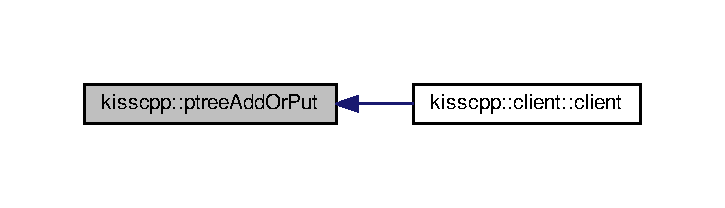
\includegraphics[width=348pt]{namespacekisscpp_a6bb122f9d1f472c12420a2ec59fdc287_icgraph}
\end{center}
\end{figure}


\hypertarget{namespacekisscpp_a36b9e65a0a3786bd85198e4530c65bf9}{\index{kisscpp@{kisscpp}!ptree\-Merge@{ptree\-Merge}}
\index{ptree\-Merge@{ptree\-Merge}!kisscpp@{kisscpp}}
\subsubsection[{ptree\-Merge}]{\setlength{\rightskip}{0pt plus 5cm}void kisscpp\-::ptree\-Merge (
\begin{DoxyParamCaption}
\item[{{\bf Boost\-Ptree} \&}]{pt1, }
\item[{{\bf Boost\-Ptree} \&}]{pt2, }
\item[{std\-::string}]{node}
\end{DoxyParamCaption}
)}}\label{namespacekisscpp_a36b9e65a0a3786bd85198e4530c65bf9}


\subsection{Variable Documentation}
\hypertarget{namespacekisscpp_a743621016edf95f7afda64b2da3bb576}{\index{kisscpp@{kisscpp}!Number\-Of\-File\-Sequince\-Digits@{Number\-Of\-File\-Sequince\-Digits}}
\index{Number\-Of\-File\-Sequince\-Digits@{Number\-Of\-File\-Sequince\-Digits}!kisscpp@{kisscpp}}
\subsubsection[{Number\-Of\-File\-Sequince\-Digits}]{\setlength{\rightskip}{0pt plus 5cm}const unsigned kisscpp\-::\-Number\-Of\-File\-Sequince\-Digits = 3}}\label{namespacekisscpp_a743621016edf95f7afda64b2da3bb576}

\hypertarget{namespacekisscpp_1_1manip}{\section{kisscpp\-:\-:manip Namespace Reference}
\label{namespacekisscpp_1_1manip}\index{kisscpp\-::manip@{kisscpp\-::manip}}
}
\subsection*{Namespaces}
\begin{DoxyCompactItemize}
\item 
\hyperlink{namespacekisscpp_1_1manip_1_1helpers}{helpers}
\end{DoxyCompactItemize}
\subsection*{Functions}
\begin{DoxyCompactItemize}
\item 
\hyperlink{classkisscpp_1_1_log_stream}{Log\-Stream} \& \hyperlink{namespacekisscpp_1_1manip_a416806b7a937a2437ffadb9b523e1cf3}{flush} (\hyperlink{classkisscpp_1_1_log_stream}{Log\-Stream} \&s)
\item 
\hyperlink{classkisscpp_1_1_log_stream}{Log\-Stream} \& \hyperlink{namespacekisscpp_1_1manip_ad682f16cb474bc7ff2c991ad2c45db66}{endl} (\hyperlink{classkisscpp_1_1_log_stream}{Log\-Stream} \&s)
\item 
\hyperlink{classkisscpp_1_1_log_stream}{Log\-Stream} \& \hyperlink{namespacekisscpp_1_1manip_a5d7a175caf56eafe6f39469a0b0ac034}{dec} (\hyperlink{classkisscpp_1_1_log_stream}{Log\-Stream} \&s)
\item 
\hyperlink{classkisscpp_1_1_log_stream}{Log\-Stream} \& \hyperlink{namespacekisscpp_1_1manip_a1463e1f81c1a4a6c6e19e883f1160059}{hex} (\hyperlink{classkisscpp_1_1_log_stream}{Log\-Stream} \&s)
\item 
\hyperlink{classkisscpp_1_1_log_stream}{Log\-Stream} \& \hyperlink{namespacekisscpp_1_1manip_a1d9bd6b119890c9396e1dce048c07032}{oct} (\hyperlink{classkisscpp_1_1_log_stream}{Log\-Stream} \&s)
\item 
\hyperlink{classkisscpp_1_1_log_stream}{Log\-Stream} \& \hyperlink{namespacekisscpp_1_1manip_a3a365ff3909fcd0d76c2f7fa4da3b2b0}{base} (\hyperlink{classkisscpp_1_1_log_stream}{Log\-Stream} \&s)
\item 
\hyperlink{classkisscpp_1_1_log_stream}{Log\-Stream} \& \hyperlink{namespacekisscpp_1_1manip_a53df3ad3d908fa67b2d4a73000241b4f}{error} (\hyperlink{classkisscpp_1_1_log_stream}{Log\-Stream} \&s, const bool permanent=false)
\item 
\hyperlink{classkisscpp_1_1_log_stream}{Log\-Stream} \& \hyperlink{namespacekisscpp_1_1manip_aff72768a5e8b0486de0cecb0bd95f3e4}{info} (\hyperlink{classkisscpp_1_1_log_stream}{Log\-Stream} \&s, const bool permanent=false)
\item 
\hyperlink{classkisscpp_1_1_log_stream}{Log\-Stream} \& \hyperlink{namespacekisscpp_1_1manip_a795be5b59b6a02e1d8f6d9d5bb41c3a4}{debug} (\hyperlink{classkisscpp_1_1_log_stream}{Log\-Stream} \&s, const bool permanent=false)
\item 
\hyperlink{classkisscpp_1_1_log_stream}{Log\-Stream} \& \hyperlink{namespacekisscpp_1_1manip_a210331dfe6a9773c4e8e1db1e889820b}{high} (\hyperlink{classkisscpp_1_1_log_stream}{Log\-Stream} \&s, const bool permanent=false)
\item 
\hyperlink{classkisscpp_1_1_log_stream}{Log\-Stream} \& \hyperlink{namespacekisscpp_1_1manip_a8f9aa3f28fd54225dee006e014efcf65}{normal} (\hyperlink{classkisscpp_1_1_log_stream}{Log\-Stream} \&s, const bool permanent=false)
\item 
\hyperlink{classkisscpp_1_1_log_stream}{Log\-Stream} \& \hyperlink{namespacekisscpp_1_1manip_a934867d04be842b8f6e9df5dfa07f40e}{low} (\hyperlink{classkisscpp_1_1_log_stream}{Log\-Stream} \&s, const bool permanent=false)
\item 
\hyperlink{classkisscpp_1_1_log_stream}{Log\-Stream} \& \hyperlink{namespacekisscpp_1_1manip_aee969aa657dcd750d102fc48a29ba516}{error\-\_\-high} (\hyperlink{classkisscpp_1_1_log_stream}{Log\-Stream} \&s, const bool permanent=false)
\item 
\hyperlink{classkisscpp_1_1_log_stream}{Log\-Stream} \& \hyperlink{namespacekisscpp_1_1manip_af7d168675689cf70931df8d3acb4b4e9}{error\-\_\-normal} (\hyperlink{classkisscpp_1_1_log_stream}{Log\-Stream} \&s, const bool permanent=false)
\item 
\hyperlink{classkisscpp_1_1_log_stream}{Log\-Stream} \& \hyperlink{namespacekisscpp_1_1manip_ab5930b238c7e5301822bc09c41120a59}{error\-\_\-low} (\hyperlink{classkisscpp_1_1_log_stream}{Log\-Stream} \&s, const bool permanent=false)
\item 
\hyperlink{classkisscpp_1_1_log_stream}{Log\-Stream} \& \hyperlink{namespacekisscpp_1_1manip_aaf086b98ab45fa8c08557762e019afb7}{debug\-\_\-high} (\hyperlink{classkisscpp_1_1_log_stream}{Log\-Stream} \&s, const bool permanent=false)
\item 
\hyperlink{classkisscpp_1_1_log_stream}{Log\-Stream} \& \hyperlink{namespacekisscpp_1_1manip_ac4893fff26af38ff60229792840064b3}{debug\-\_\-normal} (\hyperlink{classkisscpp_1_1_log_stream}{Log\-Stream} \&s, const bool permanent=false)
\item 
\hyperlink{classkisscpp_1_1_log_stream}{Log\-Stream} \& \hyperlink{namespacekisscpp_1_1manip_a14eb82a3948c039a023b254d02e4dd01}{debug\-\_\-low} (\hyperlink{classkisscpp_1_1_log_stream}{Log\-Stream} \&s, const bool permanent=false)
\item 
\hyperlink{classkisscpp_1_1_log_stream}{Log\-Stream} \& \hyperlink{namespacekisscpp_1_1manip_a0e2079570591f8a3cc788872b65c6580}{info\-\_\-high} (\hyperlink{classkisscpp_1_1_log_stream}{Log\-Stream} \&s, const bool permanent=false)
\item 
\hyperlink{classkisscpp_1_1_log_stream}{Log\-Stream} \& \hyperlink{namespacekisscpp_1_1manip_aee465aa1a8d15e1750422696f7d3dc81}{info\-\_\-normal} (\hyperlink{classkisscpp_1_1_log_stream}{Log\-Stream} \&s, const bool permanent=false)
\item 
\hyperlink{classkisscpp_1_1_log_stream}{Log\-Stream} \& \hyperlink{namespacekisscpp_1_1manip_ae246ac6f24cae0a1452a3bb8a64f538e}{info\-\_\-low} (\hyperlink{classkisscpp_1_1_log_stream}{Log\-Stream} \&s, const bool permanent=false)
\item 
\hyperlink{classkisscpp_1_1_manip_result}{Manip\-Result}$<$ std\-::string $>$ \hyperlink{namespacekisscpp_1_1manip_afa562934b333ee12ecd3219872410a8f}{ent} (const std\-::string \&ent\-\_\-name)
\item 
\hyperlink{classkisscpp_1_1_manip_result}{Manip\-Result}$<$ std\-::string $>$ \hyperlink{namespacekisscpp_1_1manip_a0660364105e23b9121ecf3d6d19858a5}{src} (const std\-::string \&source)
\end{DoxyCompactItemize}


\subsection{Function Documentation}
\hypertarget{namespacekisscpp_1_1manip_a3a365ff3909fcd0d76c2f7fa4da3b2b0}{\index{kisscpp\-::manip@{kisscpp\-::manip}!base@{base}}
\index{base@{base}!kisscpp::manip@{kisscpp\-::manip}}
\subsubsection[{base}]{\setlength{\rightskip}{0pt plus 5cm}{\bf Log\-Stream} \& kisscpp\-::manip\-::base (
\begin{DoxyParamCaption}
\item[{Log\-Stream \&}]{s}
\end{DoxyParamCaption}
)\hspace{0.3cm}{\ttfamily [inline]}}}\label{namespacekisscpp_1_1manip_a3a365ff3909fcd0d76c2f7fa4da3b2b0}


Here is the call graph for this function\-:\nopagebreak
\begin{figure}[H]
\begin{center}
\leavevmode
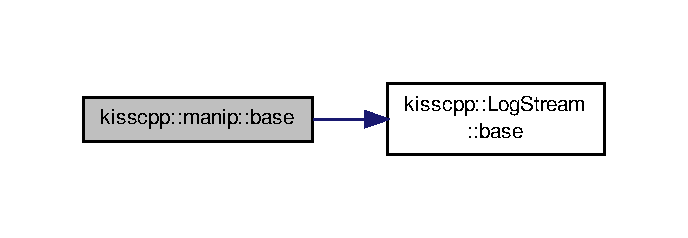
\includegraphics[width=330pt]{namespacekisscpp_1_1manip_a3a365ff3909fcd0d76c2f7fa4da3b2b0_cgraph}
\end{center}
\end{figure}


\hypertarget{namespacekisscpp_1_1manip_a795be5b59b6a02e1d8f6d9d5bb41c3a4}{\index{kisscpp\-::manip@{kisscpp\-::manip}!debug@{debug}}
\index{debug@{debug}!kisscpp::manip@{kisscpp\-::manip}}
\subsubsection[{debug}]{\setlength{\rightskip}{0pt plus 5cm}{\bf Log\-Stream} \& kisscpp\-::manip\-::debug (
\begin{DoxyParamCaption}
\item[{Log\-Stream \&}]{s, }
\item[{const bool}]{permanent = {\ttfamily false}}
\end{DoxyParamCaption}
)\hspace{0.3cm}{\ttfamily [inline]}}}\label{namespacekisscpp_1_1manip_a795be5b59b6a02e1d8f6d9d5bb41c3a4}


Here is the call graph for this function\-:\nopagebreak
\begin{figure}[H]
\begin{center}
\leavevmode
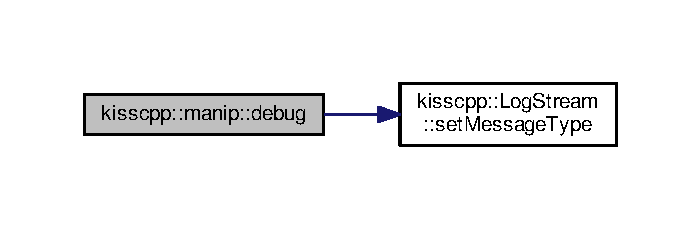
\includegraphics[width=336pt]{namespacekisscpp_1_1manip_a795be5b59b6a02e1d8f6d9d5bb41c3a4_cgraph}
\end{center}
\end{figure}




Here is the caller graph for this function\-:\nopagebreak
\begin{figure}[H]
\begin{center}
\leavevmode
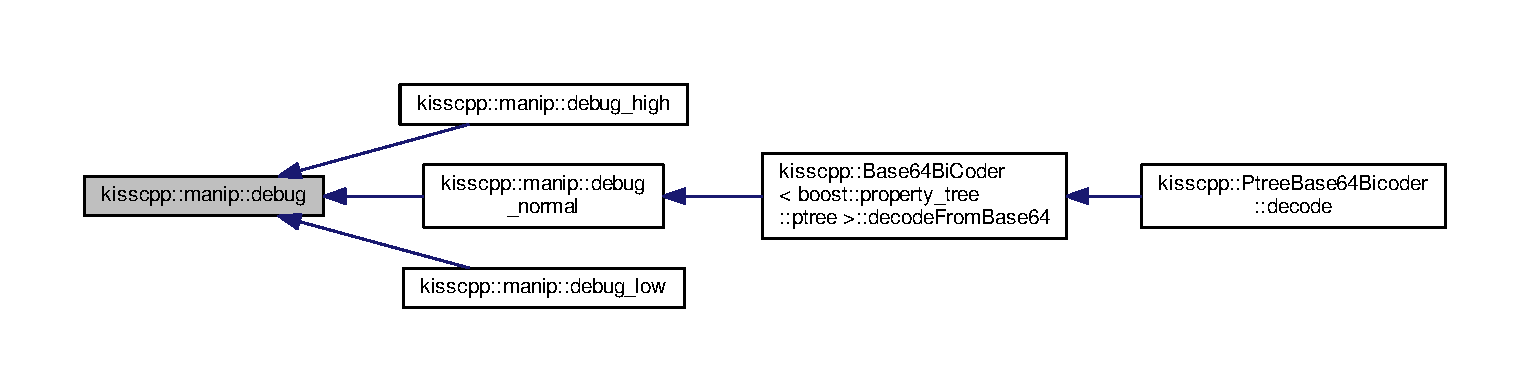
\includegraphics[width=350pt]{namespacekisscpp_1_1manip_a795be5b59b6a02e1d8f6d9d5bb41c3a4_icgraph}
\end{center}
\end{figure}


\hypertarget{namespacekisscpp_1_1manip_aaf086b98ab45fa8c08557762e019afb7}{\index{kisscpp\-::manip@{kisscpp\-::manip}!debug\-\_\-high@{debug\-\_\-high}}
\index{debug\-\_\-high@{debug\-\_\-high}!kisscpp::manip@{kisscpp\-::manip}}
\subsubsection[{debug\-\_\-high}]{\setlength{\rightskip}{0pt plus 5cm}{\bf Log\-Stream} \& kisscpp\-::manip\-::debug\-\_\-high (
\begin{DoxyParamCaption}
\item[{Log\-Stream \&}]{s, }
\item[{const bool}]{permanent = {\ttfamily false}}
\end{DoxyParamCaption}
)\hspace{0.3cm}{\ttfamily [inline]}}}\label{namespacekisscpp_1_1manip_aaf086b98ab45fa8c08557762e019afb7}


Here is the call graph for this function\-:\nopagebreak
\begin{figure}[H]
\begin{center}
\leavevmode
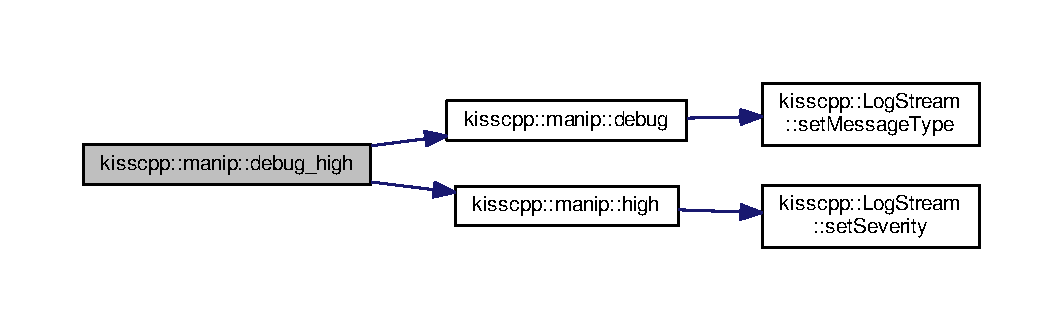
\includegraphics[width=350pt]{namespacekisscpp_1_1manip_aaf086b98ab45fa8c08557762e019afb7_cgraph}
\end{center}
\end{figure}


\hypertarget{namespacekisscpp_1_1manip_a14eb82a3948c039a023b254d02e4dd01}{\index{kisscpp\-::manip@{kisscpp\-::manip}!debug\-\_\-low@{debug\-\_\-low}}
\index{debug\-\_\-low@{debug\-\_\-low}!kisscpp::manip@{kisscpp\-::manip}}
\subsubsection[{debug\-\_\-low}]{\setlength{\rightskip}{0pt plus 5cm}{\bf Log\-Stream} \& kisscpp\-::manip\-::debug\-\_\-low (
\begin{DoxyParamCaption}
\item[{Log\-Stream \&}]{s, }
\item[{const bool}]{permanent = {\ttfamily false}}
\end{DoxyParamCaption}
)\hspace{0.3cm}{\ttfamily [inline]}}}\label{namespacekisscpp_1_1manip_a14eb82a3948c039a023b254d02e4dd01}


Here is the call graph for this function\-:\nopagebreak
\begin{figure}[H]
\begin{center}
\leavevmode
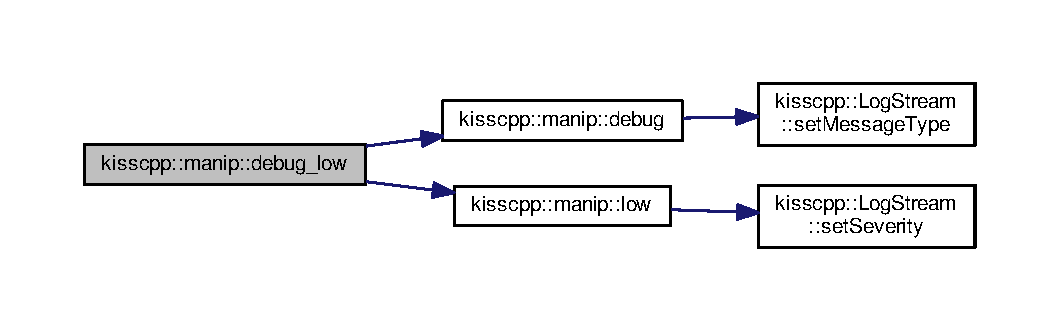
\includegraphics[width=350pt]{namespacekisscpp_1_1manip_a14eb82a3948c039a023b254d02e4dd01_cgraph}
\end{center}
\end{figure}


\hypertarget{namespacekisscpp_1_1manip_ac4893fff26af38ff60229792840064b3}{\index{kisscpp\-::manip@{kisscpp\-::manip}!debug\-\_\-normal@{debug\-\_\-normal}}
\index{debug\-\_\-normal@{debug\-\_\-normal}!kisscpp::manip@{kisscpp\-::manip}}
\subsubsection[{debug\-\_\-normal}]{\setlength{\rightskip}{0pt plus 5cm}{\bf Log\-Stream} \& kisscpp\-::manip\-::debug\-\_\-normal (
\begin{DoxyParamCaption}
\item[{Log\-Stream \&}]{s, }
\item[{const bool}]{permanent = {\ttfamily false}}
\end{DoxyParamCaption}
)\hspace{0.3cm}{\ttfamily [inline]}}}\label{namespacekisscpp_1_1manip_ac4893fff26af38ff60229792840064b3}


Here is the call graph for this function\-:\nopagebreak
\begin{figure}[H]
\begin{center}
\leavevmode
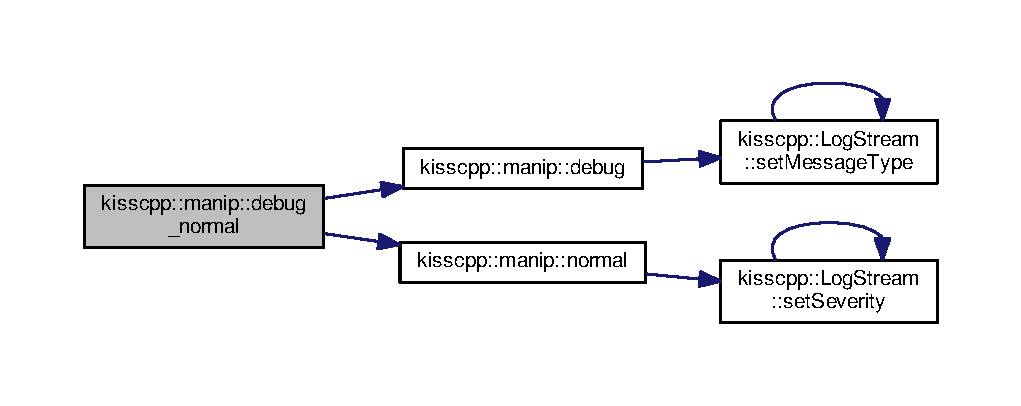
\includegraphics[width=350pt]{namespacekisscpp_1_1manip_ac4893fff26af38ff60229792840064b3_cgraph}
\end{center}
\end{figure}




Here is the caller graph for this function\-:\nopagebreak
\begin{figure}[H]
\begin{center}
\leavevmode
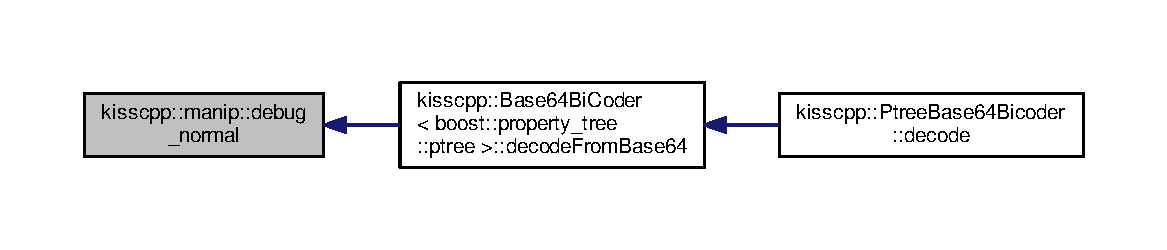
\includegraphics[width=350pt]{namespacekisscpp_1_1manip_ac4893fff26af38ff60229792840064b3_icgraph}
\end{center}
\end{figure}


\hypertarget{namespacekisscpp_1_1manip_a5d7a175caf56eafe6f39469a0b0ac034}{\index{kisscpp\-::manip@{kisscpp\-::manip}!dec@{dec}}
\index{dec@{dec}!kisscpp::manip@{kisscpp\-::manip}}
\subsubsection[{dec}]{\setlength{\rightskip}{0pt plus 5cm}{\bf Log\-Stream} \& kisscpp\-::manip\-::dec (
\begin{DoxyParamCaption}
\item[{Log\-Stream \&}]{s}
\end{DoxyParamCaption}
)\hspace{0.3cm}{\ttfamily [inline]}}}\label{namespacekisscpp_1_1manip_a5d7a175caf56eafe6f39469a0b0ac034}


Here is the call graph for this function\-:\nopagebreak
\begin{figure}[H]
\begin{center}
\leavevmode
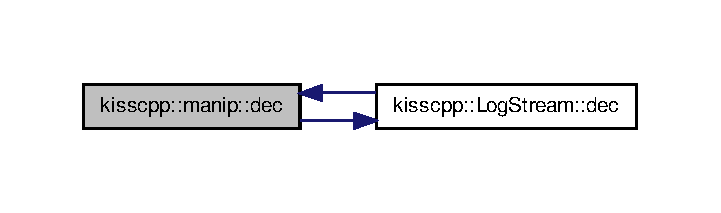
\includegraphics[width=346pt]{namespacekisscpp_1_1manip_a5d7a175caf56eafe6f39469a0b0ac034_cgraph}
\end{center}
\end{figure}




Here is the caller graph for this function\-:\nopagebreak
\begin{figure}[H]
\begin{center}
\leavevmode
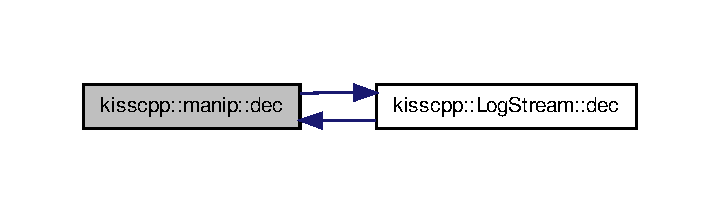
\includegraphics[width=346pt]{namespacekisscpp_1_1manip_a5d7a175caf56eafe6f39469a0b0ac034_icgraph}
\end{center}
\end{figure}


\hypertarget{namespacekisscpp_1_1manip_ad682f16cb474bc7ff2c991ad2c45db66}{\index{kisscpp\-::manip@{kisscpp\-::manip}!endl@{endl}}
\index{endl@{endl}!kisscpp::manip@{kisscpp\-::manip}}
\subsubsection[{endl}]{\setlength{\rightskip}{0pt plus 5cm}{\bf Log\-Stream} \& kisscpp\-::manip\-::endl (
\begin{DoxyParamCaption}
\item[{Log\-Stream \&}]{s}
\end{DoxyParamCaption}
)\hspace{0.3cm}{\ttfamily [inline]}}}\label{namespacekisscpp_1_1manip_ad682f16cb474bc7ff2c991ad2c45db66}


Here is the call graph for this function\-:\nopagebreak
\begin{figure}[H]
\begin{center}
\leavevmode
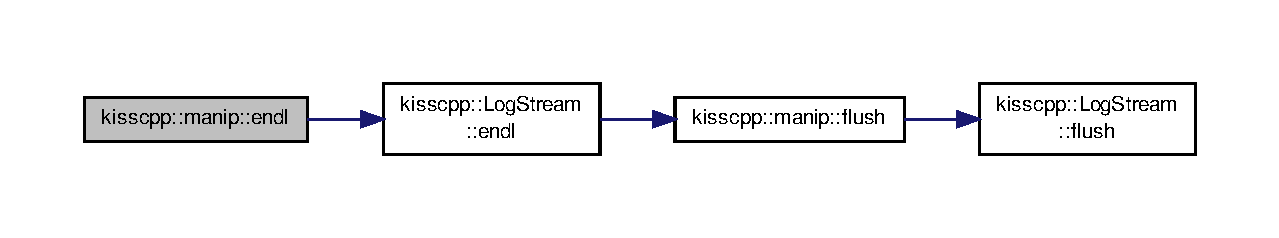
\includegraphics[width=328pt]{namespacekisscpp_1_1manip_ad682f16cb474bc7ff2c991ad2c45db66_cgraph}
\end{center}
\end{figure}




Here is the caller graph for this function\-:\nopagebreak
\begin{figure}[H]
\begin{center}
\leavevmode
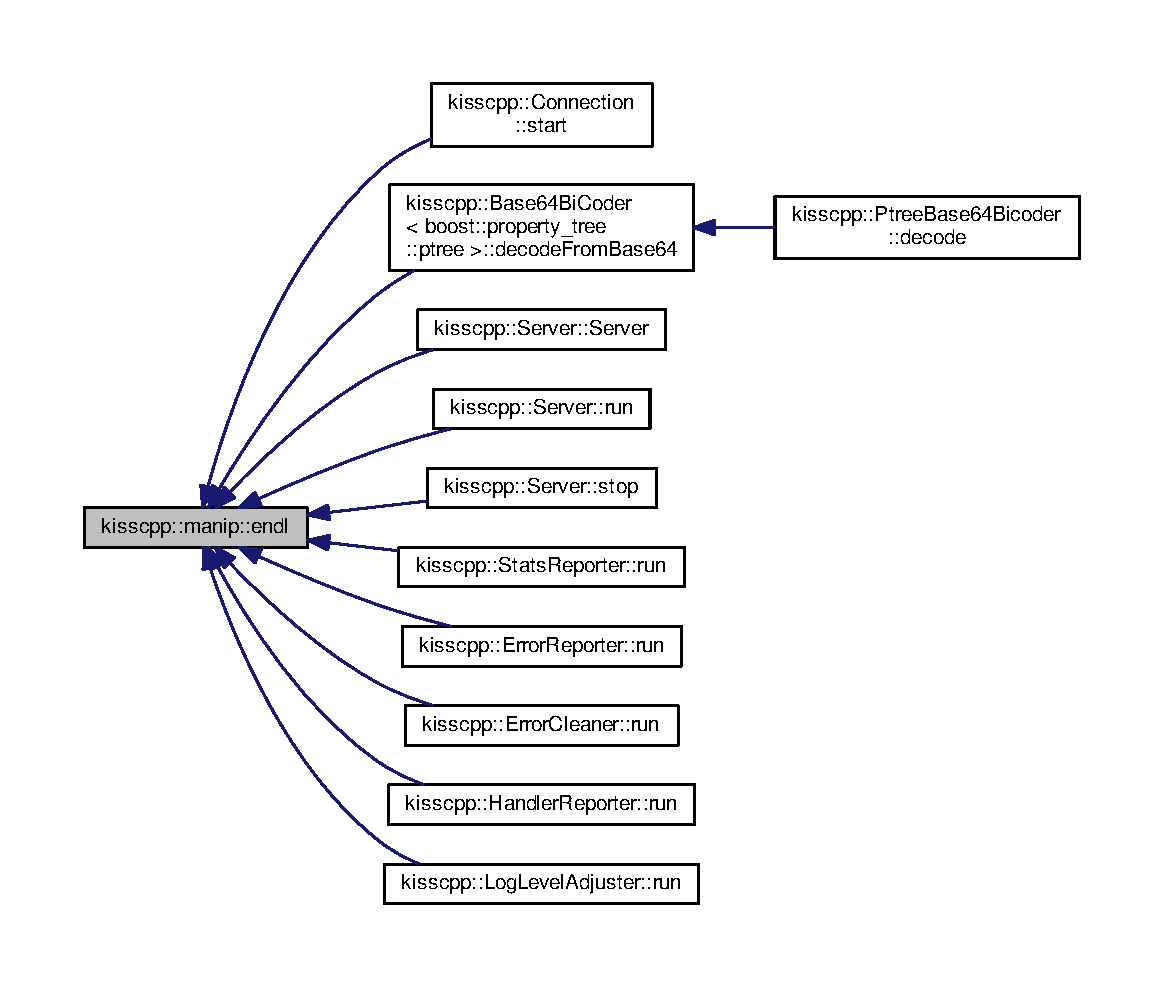
\includegraphics[width=350pt]{namespacekisscpp_1_1manip_ad682f16cb474bc7ff2c991ad2c45db66_icgraph}
\end{center}
\end{figure}


\hypertarget{namespacekisscpp_1_1manip_afa562934b333ee12ecd3219872410a8f}{\index{kisscpp\-::manip@{kisscpp\-::manip}!ent@{ent}}
\index{ent@{ent}!kisscpp::manip@{kisscpp\-::manip}}
\subsubsection[{ent}]{\setlength{\rightskip}{0pt plus 5cm}{\bf Manip\-Result}$<$ std\-::string $>$ kisscpp\-::manip\-::ent (
\begin{DoxyParamCaption}
\item[{const std\-::string \&}]{ent\-\_\-name}
\end{DoxyParamCaption}
)\hspace{0.3cm}{\ttfamily [inline]}}}\label{namespacekisscpp_1_1manip_afa562934b333ee12ecd3219872410a8f}


Here is the call graph for this function\-:\nopagebreak
\begin{figure}[H]
\begin{center}
\leavevmode
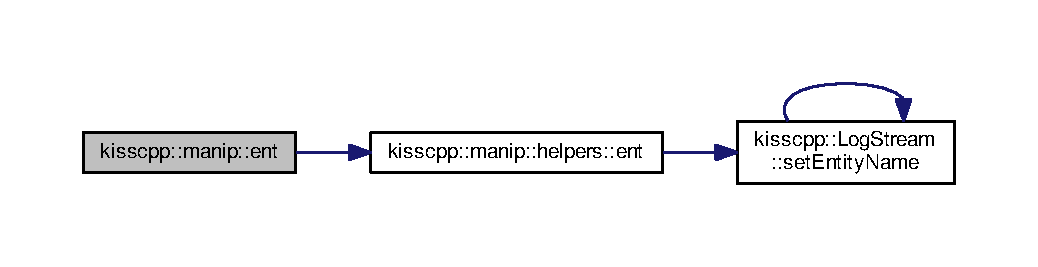
\includegraphics[width=350pt]{namespacekisscpp_1_1manip_afa562934b333ee12ecd3219872410a8f_cgraph}
\end{center}
\end{figure}


\hypertarget{namespacekisscpp_1_1manip_a53df3ad3d908fa67b2d4a73000241b4f}{\index{kisscpp\-::manip@{kisscpp\-::manip}!error@{error}}
\index{error@{error}!kisscpp::manip@{kisscpp\-::manip}}
\subsubsection[{error}]{\setlength{\rightskip}{0pt plus 5cm}{\bf Log\-Stream} \& kisscpp\-::manip\-::error (
\begin{DoxyParamCaption}
\item[{Log\-Stream \&}]{s, }
\item[{const bool}]{permanent = {\ttfamily false}}
\end{DoxyParamCaption}
)\hspace{0.3cm}{\ttfamily [inline]}}}\label{namespacekisscpp_1_1manip_a53df3ad3d908fa67b2d4a73000241b4f}


Here is the call graph for this function\-:\nopagebreak
\begin{figure}[H]
\begin{center}
\leavevmode
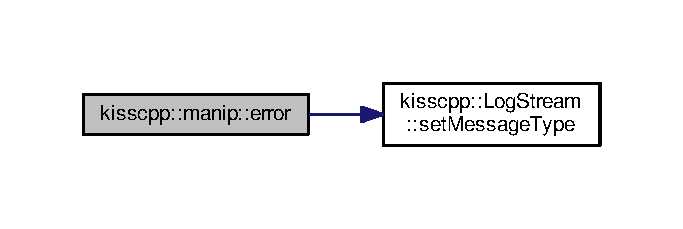
\includegraphics[width=328pt]{namespacekisscpp_1_1manip_a53df3ad3d908fa67b2d4a73000241b4f_cgraph}
\end{center}
\end{figure}




Here is the caller graph for this function\-:\nopagebreak
\begin{figure}[H]
\begin{center}
\leavevmode
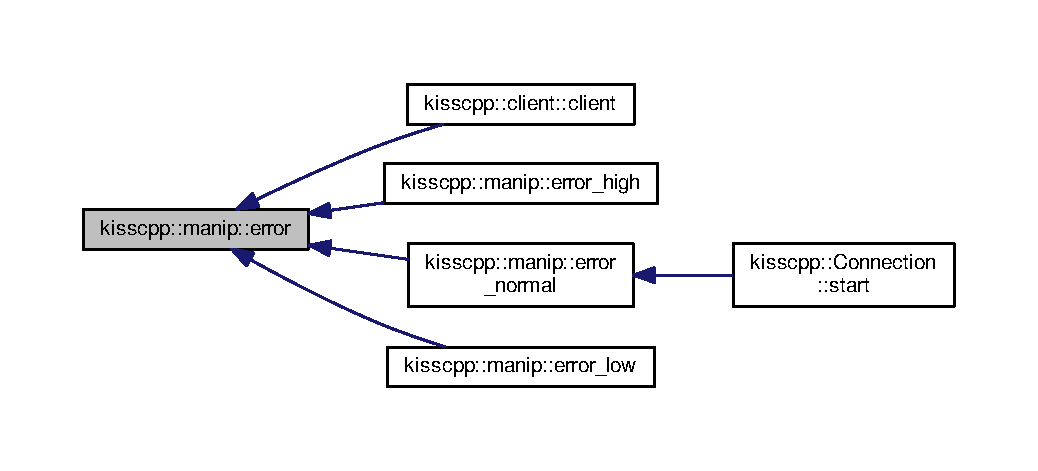
\includegraphics[width=350pt]{namespacekisscpp_1_1manip_a53df3ad3d908fa67b2d4a73000241b4f_icgraph}
\end{center}
\end{figure}


\hypertarget{namespacekisscpp_1_1manip_aee969aa657dcd750d102fc48a29ba516}{\index{kisscpp\-::manip@{kisscpp\-::manip}!error\-\_\-high@{error\-\_\-high}}
\index{error\-\_\-high@{error\-\_\-high}!kisscpp::manip@{kisscpp\-::manip}}
\subsubsection[{error\-\_\-high}]{\setlength{\rightskip}{0pt plus 5cm}{\bf Log\-Stream} \& kisscpp\-::manip\-::error\-\_\-high (
\begin{DoxyParamCaption}
\item[{Log\-Stream \&}]{s, }
\item[{const bool}]{permanent = {\ttfamily false}}
\end{DoxyParamCaption}
)\hspace{0.3cm}{\ttfamily [inline]}}}\label{namespacekisscpp_1_1manip_aee969aa657dcd750d102fc48a29ba516}


Here is the call graph for this function\-:\nopagebreak
\begin{figure}[H]
\begin{center}
\leavevmode
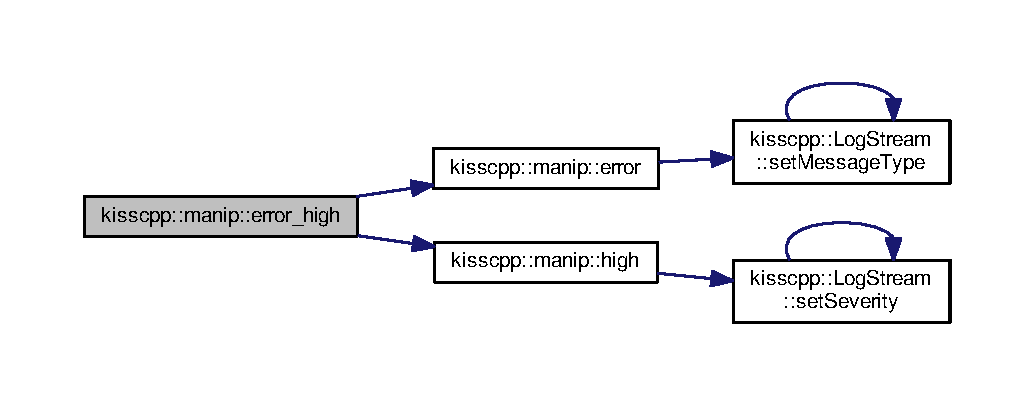
\includegraphics[width=350pt]{namespacekisscpp_1_1manip_aee969aa657dcd750d102fc48a29ba516_cgraph}
\end{center}
\end{figure}


\hypertarget{namespacekisscpp_1_1manip_ab5930b238c7e5301822bc09c41120a59}{\index{kisscpp\-::manip@{kisscpp\-::manip}!error\-\_\-low@{error\-\_\-low}}
\index{error\-\_\-low@{error\-\_\-low}!kisscpp::manip@{kisscpp\-::manip}}
\subsubsection[{error\-\_\-low}]{\setlength{\rightskip}{0pt plus 5cm}{\bf Log\-Stream} \& kisscpp\-::manip\-::error\-\_\-low (
\begin{DoxyParamCaption}
\item[{Log\-Stream \&}]{s, }
\item[{const bool}]{permanent = {\ttfamily false}}
\end{DoxyParamCaption}
)\hspace{0.3cm}{\ttfamily [inline]}}}\label{namespacekisscpp_1_1manip_ab5930b238c7e5301822bc09c41120a59}


Here is the call graph for this function\-:\nopagebreak
\begin{figure}[H]
\begin{center}
\leavevmode
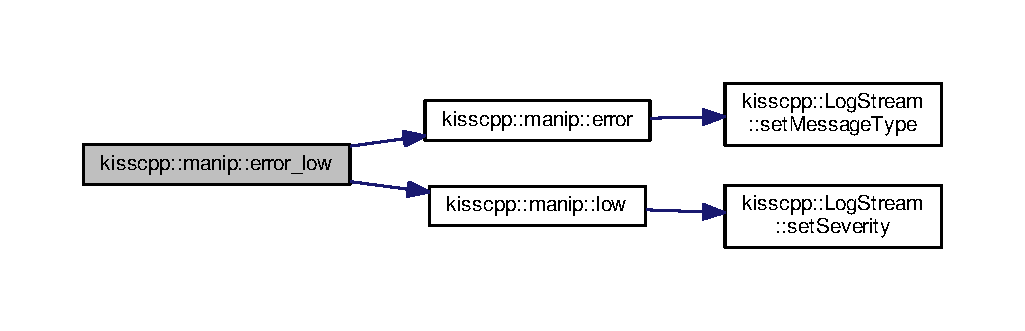
\includegraphics[width=350pt]{namespacekisscpp_1_1manip_ab5930b238c7e5301822bc09c41120a59_cgraph}
\end{center}
\end{figure}


\hypertarget{namespacekisscpp_1_1manip_af7d168675689cf70931df8d3acb4b4e9}{\index{kisscpp\-::manip@{kisscpp\-::manip}!error\-\_\-normal@{error\-\_\-normal}}
\index{error\-\_\-normal@{error\-\_\-normal}!kisscpp::manip@{kisscpp\-::manip}}
\subsubsection[{error\-\_\-normal}]{\setlength{\rightskip}{0pt plus 5cm}{\bf Log\-Stream} \& kisscpp\-::manip\-::error\-\_\-normal (
\begin{DoxyParamCaption}
\item[{Log\-Stream \&}]{s, }
\item[{const bool}]{permanent = {\ttfamily false}}
\end{DoxyParamCaption}
)\hspace{0.3cm}{\ttfamily [inline]}}}\label{namespacekisscpp_1_1manip_af7d168675689cf70931df8d3acb4b4e9}


Here is the call graph for this function\-:\nopagebreak
\begin{figure}[H]
\begin{center}
\leavevmode
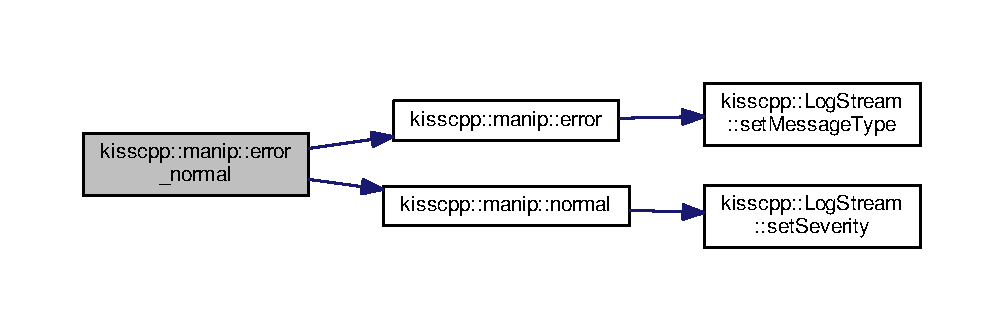
\includegraphics[width=350pt]{namespacekisscpp_1_1manip_af7d168675689cf70931df8d3acb4b4e9_cgraph}
\end{center}
\end{figure}




Here is the caller graph for this function\-:\nopagebreak
\begin{figure}[H]
\begin{center}
\leavevmode
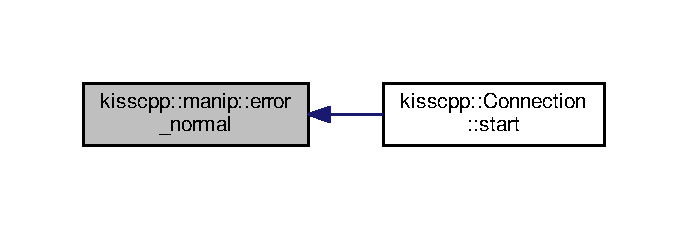
\includegraphics[width=330pt]{namespacekisscpp_1_1manip_af7d168675689cf70931df8d3acb4b4e9_icgraph}
\end{center}
\end{figure}


\hypertarget{namespacekisscpp_1_1manip_a416806b7a937a2437ffadb9b523e1cf3}{\index{kisscpp\-::manip@{kisscpp\-::manip}!flush@{flush}}
\index{flush@{flush}!kisscpp::manip@{kisscpp\-::manip}}
\subsubsection[{flush}]{\setlength{\rightskip}{0pt plus 5cm}{\bf Log\-Stream} \& kisscpp\-::manip\-::flush (
\begin{DoxyParamCaption}
\item[{Log\-Stream \&}]{s}
\end{DoxyParamCaption}
)\hspace{0.3cm}{\ttfamily [inline]}}}\label{namespacekisscpp_1_1manip_a416806b7a937a2437ffadb9b523e1cf3}


Here is the call graph for this function\-:\nopagebreak
\begin{figure}[H]
\begin{center}
\leavevmode
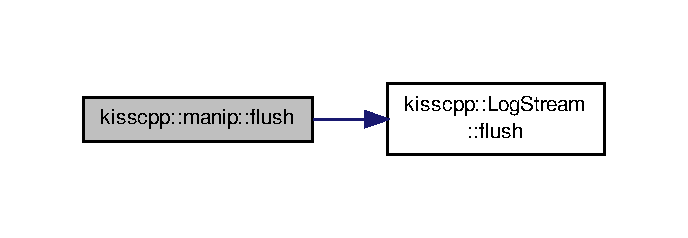
\includegraphics[width=330pt]{namespacekisscpp_1_1manip_a416806b7a937a2437ffadb9b523e1cf3_cgraph}
\end{center}
\end{figure}




Here is the caller graph for this function\-:\nopagebreak
\begin{figure}[H]
\begin{center}
\leavevmode
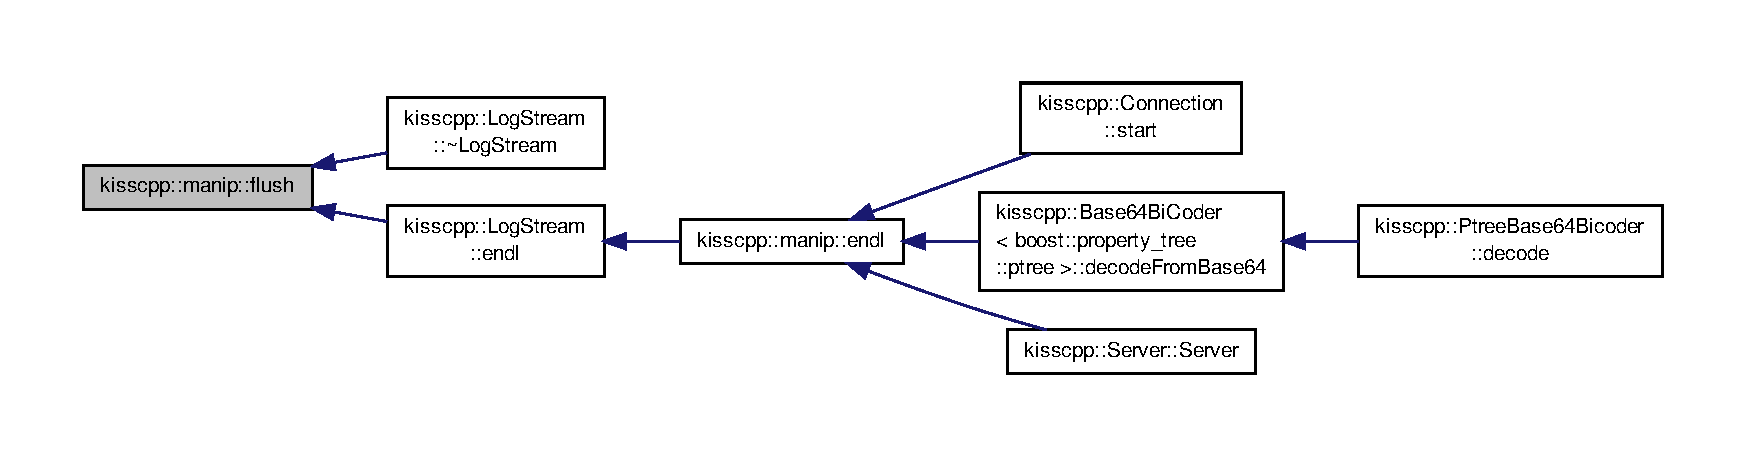
\includegraphics[width=336pt]{namespacekisscpp_1_1manip_a416806b7a937a2437ffadb9b523e1cf3_icgraph}
\end{center}
\end{figure}


\hypertarget{namespacekisscpp_1_1manip_a1463e1f81c1a4a6c6e19e883f1160059}{\index{kisscpp\-::manip@{kisscpp\-::manip}!hex@{hex}}
\index{hex@{hex}!kisscpp::manip@{kisscpp\-::manip}}
\subsubsection[{hex}]{\setlength{\rightskip}{0pt plus 5cm}{\bf Log\-Stream} \& kisscpp\-::manip\-::hex (
\begin{DoxyParamCaption}
\item[{Log\-Stream \&}]{s}
\end{DoxyParamCaption}
)\hspace{0.3cm}{\ttfamily [inline]}}}\label{namespacekisscpp_1_1manip_a1463e1f81c1a4a6c6e19e883f1160059}


Here is the call graph for this function\-:\nopagebreak
\begin{figure}[H]
\begin{center}
\leavevmode
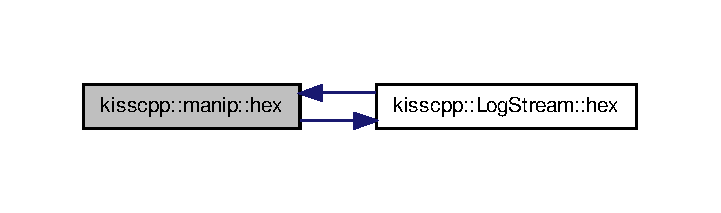
\includegraphics[width=346pt]{namespacekisscpp_1_1manip_a1463e1f81c1a4a6c6e19e883f1160059_cgraph}
\end{center}
\end{figure}




Here is the caller graph for this function\-:\nopagebreak
\begin{figure}[H]
\begin{center}
\leavevmode
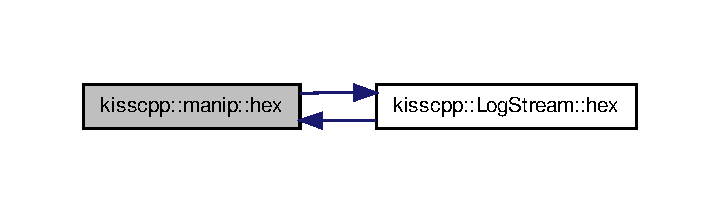
\includegraphics[width=346pt]{namespacekisscpp_1_1manip_a1463e1f81c1a4a6c6e19e883f1160059_icgraph}
\end{center}
\end{figure}


\hypertarget{namespacekisscpp_1_1manip_a210331dfe6a9773c4e8e1db1e889820b}{\index{kisscpp\-::manip@{kisscpp\-::manip}!high@{high}}
\index{high@{high}!kisscpp::manip@{kisscpp\-::manip}}
\subsubsection[{high}]{\setlength{\rightskip}{0pt plus 5cm}{\bf Log\-Stream} \& kisscpp\-::manip\-::high (
\begin{DoxyParamCaption}
\item[{Log\-Stream \&}]{s, }
\item[{const bool}]{permanent = {\ttfamily false}}
\end{DoxyParamCaption}
)\hspace{0.3cm}{\ttfamily [inline]}}}\label{namespacekisscpp_1_1manip_a210331dfe6a9773c4e8e1db1e889820b}


Here is the call graph for this function\-:\nopagebreak
\begin{figure}[H]
\begin{center}
\leavevmode
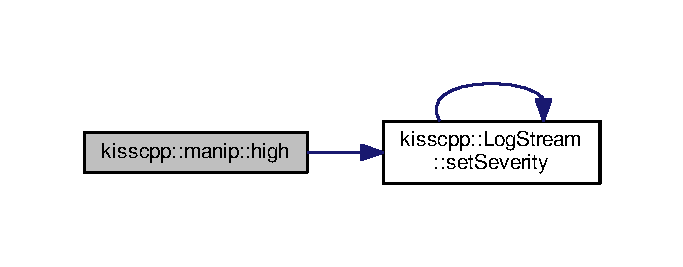
\includegraphics[width=328pt]{namespacekisscpp_1_1manip_a210331dfe6a9773c4e8e1db1e889820b_cgraph}
\end{center}
\end{figure}




Here is the caller graph for this function\-:\nopagebreak
\begin{figure}[H]
\begin{center}
\leavevmode
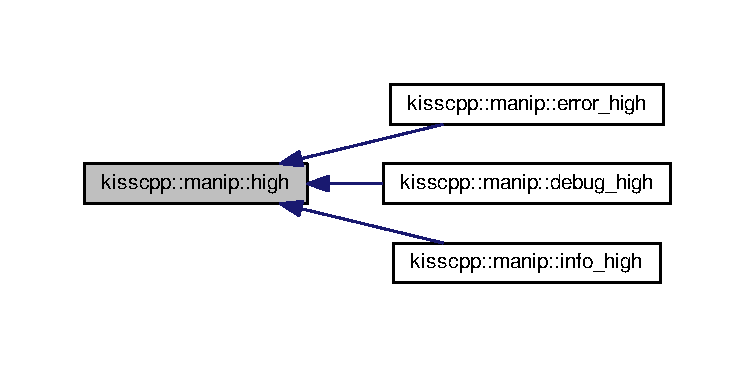
\includegraphics[width=350pt]{namespacekisscpp_1_1manip_a210331dfe6a9773c4e8e1db1e889820b_icgraph}
\end{center}
\end{figure}


\hypertarget{namespacekisscpp_1_1manip_aff72768a5e8b0486de0cecb0bd95f3e4}{\index{kisscpp\-::manip@{kisscpp\-::manip}!info@{info}}
\index{info@{info}!kisscpp::manip@{kisscpp\-::manip}}
\subsubsection[{info}]{\setlength{\rightskip}{0pt plus 5cm}{\bf Log\-Stream} \& kisscpp\-::manip\-::info (
\begin{DoxyParamCaption}
\item[{Log\-Stream \&}]{s, }
\item[{const bool}]{permanent = {\ttfamily false}}
\end{DoxyParamCaption}
)\hspace{0.3cm}{\ttfamily [inline]}}}\label{namespacekisscpp_1_1manip_aff72768a5e8b0486de0cecb0bd95f3e4}


Here is the call graph for this function\-:\nopagebreak
\begin{figure}[H]
\begin{center}
\leavevmode
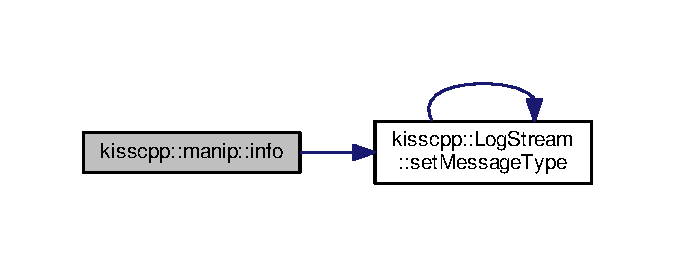
\includegraphics[width=324pt]{namespacekisscpp_1_1manip_aff72768a5e8b0486de0cecb0bd95f3e4_cgraph}
\end{center}
\end{figure}




Here is the caller graph for this function\-:\nopagebreak
\begin{figure}[H]
\begin{center}
\leavevmode
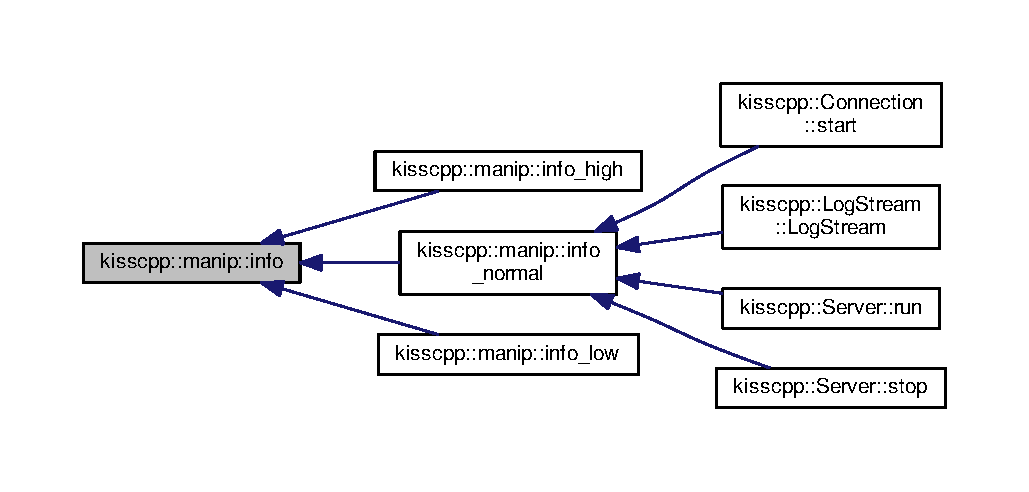
\includegraphics[width=350pt]{namespacekisscpp_1_1manip_aff72768a5e8b0486de0cecb0bd95f3e4_icgraph}
\end{center}
\end{figure}


\hypertarget{namespacekisscpp_1_1manip_a0e2079570591f8a3cc788872b65c6580}{\index{kisscpp\-::manip@{kisscpp\-::manip}!info\-\_\-high@{info\-\_\-high}}
\index{info\-\_\-high@{info\-\_\-high}!kisscpp::manip@{kisscpp\-::manip}}
\subsubsection[{info\-\_\-high}]{\setlength{\rightskip}{0pt plus 5cm}{\bf Log\-Stream} \& kisscpp\-::manip\-::info\-\_\-high (
\begin{DoxyParamCaption}
\item[{Log\-Stream \&}]{s, }
\item[{const bool}]{permanent = {\ttfamily false}}
\end{DoxyParamCaption}
)\hspace{0.3cm}{\ttfamily [inline]}}}\label{namespacekisscpp_1_1manip_a0e2079570591f8a3cc788872b65c6580}


Here is the call graph for this function\-:\nopagebreak
\begin{figure}[H]
\begin{center}
\leavevmode
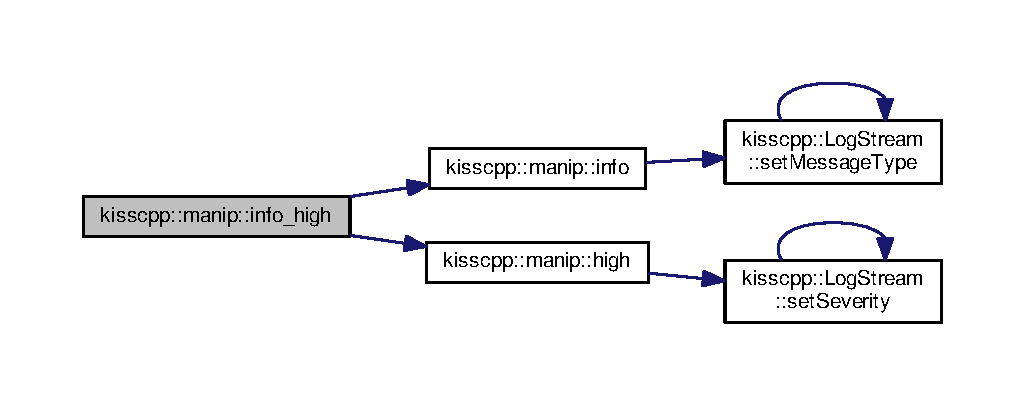
\includegraphics[width=350pt]{namespacekisscpp_1_1manip_a0e2079570591f8a3cc788872b65c6580_cgraph}
\end{center}
\end{figure}


\hypertarget{namespacekisscpp_1_1manip_ae246ac6f24cae0a1452a3bb8a64f538e}{\index{kisscpp\-::manip@{kisscpp\-::manip}!info\-\_\-low@{info\-\_\-low}}
\index{info\-\_\-low@{info\-\_\-low}!kisscpp::manip@{kisscpp\-::manip}}
\subsubsection[{info\-\_\-low}]{\setlength{\rightskip}{0pt plus 5cm}{\bf Log\-Stream} \& kisscpp\-::manip\-::info\-\_\-low (
\begin{DoxyParamCaption}
\item[{Log\-Stream \&}]{s, }
\item[{const bool}]{permanent = {\ttfamily false}}
\end{DoxyParamCaption}
)\hspace{0.3cm}{\ttfamily [inline]}}}\label{namespacekisscpp_1_1manip_ae246ac6f24cae0a1452a3bb8a64f538e}


Here is the call graph for this function\-:\nopagebreak
\begin{figure}[H]
\begin{center}
\leavevmode
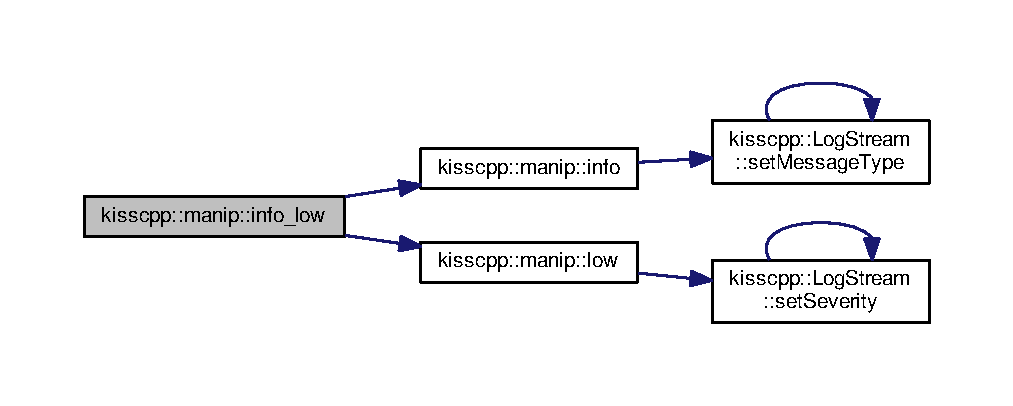
\includegraphics[width=350pt]{namespacekisscpp_1_1manip_ae246ac6f24cae0a1452a3bb8a64f538e_cgraph}
\end{center}
\end{figure}


\hypertarget{namespacekisscpp_1_1manip_aee465aa1a8d15e1750422696f7d3dc81}{\index{kisscpp\-::manip@{kisscpp\-::manip}!info\-\_\-normal@{info\-\_\-normal}}
\index{info\-\_\-normal@{info\-\_\-normal}!kisscpp::manip@{kisscpp\-::manip}}
\subsubsection[{info\-\_\-normal}]{\setlength{\rightskip}{0pt plus 5cm}{\bf Log\-Stream} \& kisscpp\-::manip\-::info\-\_\-normal (
\begin{DoxyParamCaption}
\item[{Log\-Stream \&}]{s, }
\item[{const bool}]{permanent = {\ttfamily false}}
\end{DoxyParamCaption}
)\hspace{0.3cm}{\ttfamily [inline]}}}\label{namespacekisscpp_1_1manip_aee465aa1a8d15e1750422696f7d3dc81}


Here is the call graph for this function\-:\nopagebreak
\begin{figure}[H]
\begin{center}
\leavevmode
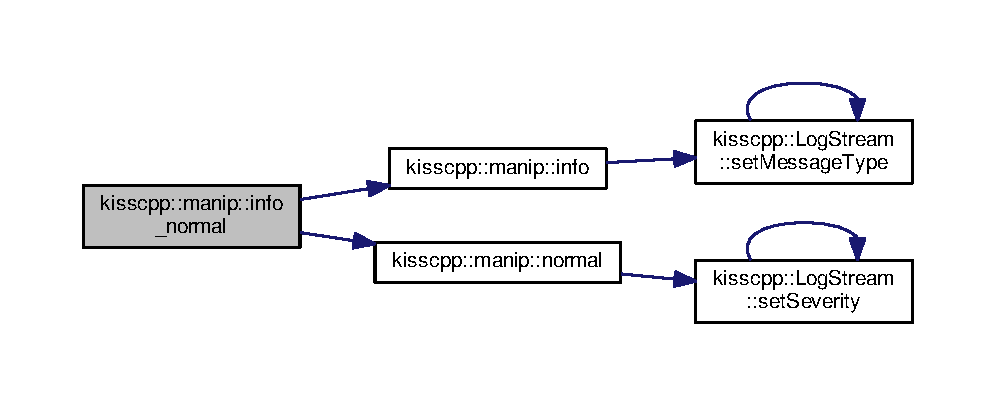
\includegraphics[width=350pt]{namespacekisscpp_1_1manip_aee465aa1a8d15e1750422696f7d3dc81_cgraph}
\end{center}
\end{figure}




Here is the caller graph for this function\-:\nopagebreak
\begin{figure}[H]
\begin{center}
\leavevmode
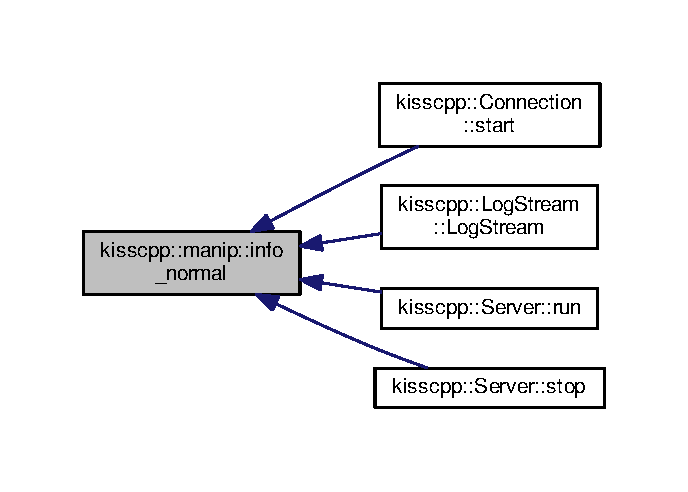
\includegraphics[width=330pt]{namespacekisscpp_1_1manip_aee465aa1a8d15e1750422696f7d3dc81_icgraph}
\end{center}
\end{figure}


\hypertarget{namespacekisscpp_1_1manip_a934867d04be842b8f6e9df5dfa07f40e}{\index{kisscpp\-::manip@{kisscpp\-::manip}!low@{low}}
\index{low@{low}!kisscpp::manip@{kisscpp\-::manip}}
\subsubsection[{low}]{\setlength{\rightskip}{0pt plus 5cm}{\bf Log\-Stream} \& kisscpp\-::manip\-::low (
\begin{DoxyParamCaption}
\item[{Log\-Stream \&}]{s, }
\item[{const bool}]{permanent = {\ttfamily false}}
\end{DoxyParamCaption}
)\hspace{0.3cm}{\ttfamily [inline]}}}\label{namespacekisscpp_1_1manip_a934867d04be842b8f6e9df5dfa07f40e}


Here is the call graph for this function\-:\nopagebreak
\begin{figure}[H]
\begin{center}
\leavevmode
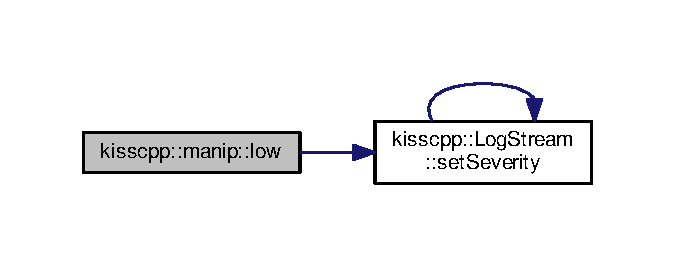
\includegraphics[width=324pt]{namespacekisscpp_1_1manip_a934867d04be842b8f6e9df5dfa07f40e_cgraph}
\end{center}
\end{figure}




Here is the caller graph for this function\-:\nopagebreak
\begin{figure}[H]
\begin{center}
\leavevmode
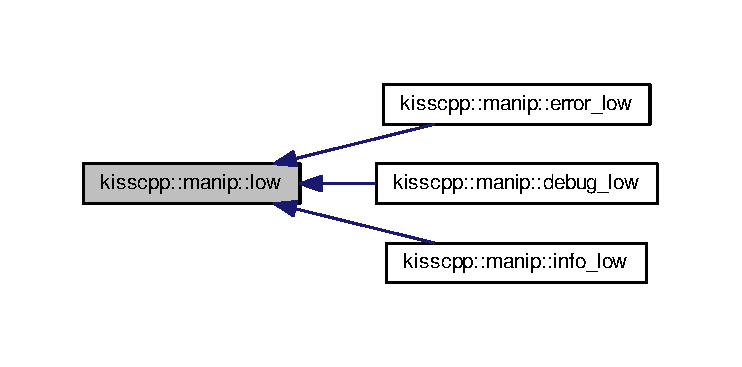
\includegraphics[width=350pt]{namespacekisscpp_1_1manip_a934867d04be842b8f6e9df5dfa07f40e_icgraph}
\end{center}
\end{figure}


\hypertarget{namespacekisscpp_1_1manip_a8f9aa3f28fd54225dee006e014efcf65}{\index{kisscpp\-::manip@{kisscpp\-::manip}!normal@{normal}}
\index{normal@{normal}!kisscpp::manip@{kisscpp\-::manip}}
\subsubsection[{normal}]{\setlength{\rightskip}{0pt plus 5cm}{\bf Log\-Stream} \& kisscpp\-::manip\-::normal (
\begin{DoxyParamCaption}
\item[{Log\-Stream \&}]{s, }
\item[{const bool}]{permanent = {\ttfamily false}}
\end{DoxyParamCaption}
)\hspace{0.3cm}{\ttfamily [inline]}}}\label{namespacekisscpp_1_1manip_a8f9aa3f28fd54225dee006e014efcf65}


Here is the call graph for this function\-:\nopagebreak
\begin{figure}[H]
\begin{center}
\leavevmode
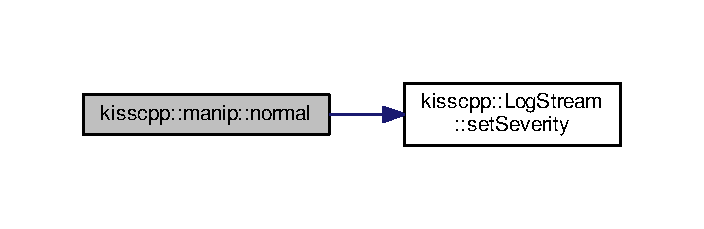
\includegraphics[width=338pt]{namespacekisscpp_1_1manip_a8f9aa3f28fd54225dee006e014efcf65_cgraph}
\end{center}
\end{figure}




Here is the caller graph for this function\-:\nopagebreak
\begin{figure}[H]
\begin{center}
\leavevmode
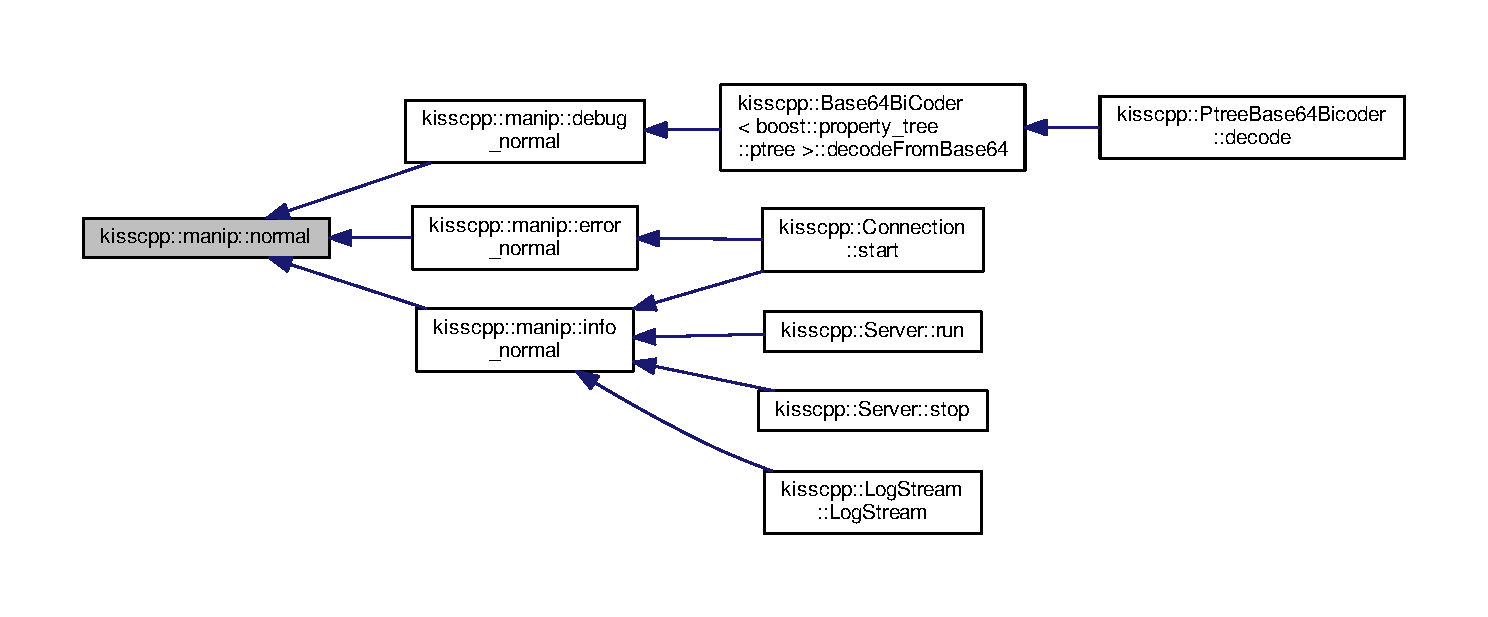
\includegraphics[width=350pt]{namespacekisscpp_1_1manip_a8f9aa3f28fd54225dee006e014efcf65_icgraph}
\end{center}
\end{figure}


\hypertarget{namespacekisscpp_1_1manip_a1d9bd6b119890c9396e1dce048c07032}{\index{kisscpp\-::manip@{kisscpp\-::manip}!oct@{oct}}
\index{oct@{oct}!kisscpp::manip@{kisscpp\-::manip}}
\subsubsection[{oct}]{\setlength{\rightskip}{0pt plus 5cm}{\bf Log\-Stream} \& kisscpp\-::manip\-::oct (
\begin{DoxyParamCaption}
\item[{Log\-Stream \&}]{s}
\end{DoxyParamCaption}
)\hspace{0.3cm}{\ttfamily [inline]}}}\label{namespacekisscpp_1_1manip_a1d9bd6b119890c9396e1dce048c07032}


Here is the call graph for this function\-:\nopagebreak
\begin{figure}[H]
\begin{center}
\leavevmode
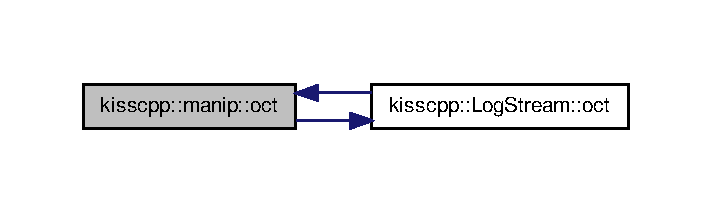
\includegraphics[width=342pt]{namespacekisscpp_1_1manip_a1d9bd6b119890c9396e1dce048c07032_cgraph}
\end{center}
\end{figure}




Here is the caller graph for this function\-:\nopagebreak
\begin{figure}[H]
\begin{center}
\leavevmode
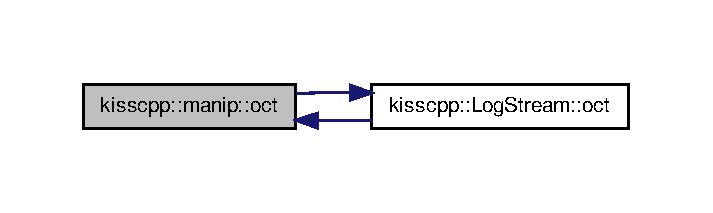
\includegraphics[width=342pt]{namespacekisscpp_1_1manip_a1d9bd6b119890c9396e1dce048c07032_icgraph}
\end{center}
\end{figure}


\hypertarget{namespacekisscpp_1_1manip_a0660364105e23b9121ecf3d6d19858a5}{\index{kisscpp\-::manip@{kisscpp\-::manip}!src@{src}}
\index{src@{src}!kisscpp::manip@{kisscpp\-::manip}}
\subsubsection[{src}]{\setlength{\rightskip}{0pt plus 5cm}{\bf Manip\-Result}$<$ std\-::string $>$ kisscpp\-::manip\-::src (
\begin{DoxyParamCaption}
\item[{const std\-::string \&}]{source}
\end{DoxyParamCaption}
)\hspace{0.3cm}{\ttfamily [inline]}}}\label{namespacekisscpp_1_1manip_a0660364105e23b9121ecf3d6d19858a5}


Here is the call graph for this function\-:\nopagebreak
\begin{figure}[H]
\begin{center}
\leavevmode
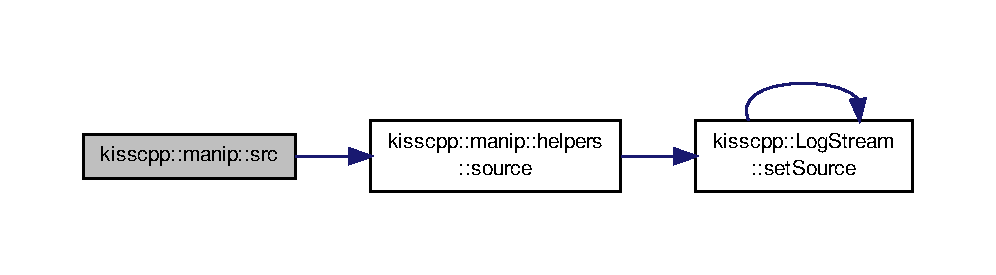
\includegraphics[width=350pt]{namespacekisscpp_1_1manip_a0660364105e23b9121ecf3d6d19858a5_cgraph}
\end{center}
\end{figure}



\hypertarget{namespacekisscpp_1_1manip_1_1helpers}{\section{kisscpp\-:\-:manip\-:\-:helpers Namespace Reference}
\label{namespacekisscpp_1_1manip_1_1helpers}\index{kisscpp\-::manip\-::helpers@{kisscpp\-::manip\-::helpers}}
}
\subsection*{Functions}
\begin{DoxyCompactItemize}
\item 
\hyperlink{classkisscpp_1_1_log_stream}{Log\-Stream} \& \hyperlink{namespacekisscpp_1_1manip_1_1helpers_a3734b7b27eea582e8d748c99ca2da137}{mask} (\hyperlink{classkisscpp_1_1_log_stream}{Log\-Stream} \&s, uint32\-\_\-t m)
\item 
\hyperlink{classkisscpp_1_1_log_stream}{Log\-Stream} \& \hyperlink{namespacekisscpp_1_1manip_1_1helpers_ad663c6941c8fb0937690a6468cc4b350}{ent} (\hyperlink{classkisscpp_1_1_log_stream}{Log\-Stream} \&s, std\-::string ent\-\_\-name)
\item 
\hyperlink{classkisscpp_1_1_log_stream}{Log\-Stream} \& \hyperlink{namespacekisscpp_1_1manip_1_1helpers_a97784407250b5ea47c0b20441a7472e5}{source} (\hyperlink{classkisscpp_1_1_log_stream}{Log\-Stream} \&s, std\-::string source)
\end{DoxyCompactItemize}


\subsection{Function Documentation}
\hypertarget{namespacekisscpp_1_1manip_1_1helpers_ad663c6941c8fb0937690a6468cc4b350}{\index{kisscpp\-::manip\-::helpers@{kisscpp\-::manip\-::helpers}!ent@{ent}}
\index{ent@{ent}!kisscpp::manip::helpers@{kisscpp\-::manip\-::helpers}}
\subsubsection[{ent}]{\setlength{\rightskip}{0pt plus 5cm}{\bf Log\-Stream} \& kisscpp\-::manip\-::helpers\-::ent (
\begin{DoxyParamCaption}
\item[{Log\-Stream \&}]{s, }
\item[{std\-::string}]{ent\-\_\-name}
\end{DoxyParamCaption}
)\hspace{0.3cm}{\ttfamily [inline]}}}\label{namespacekisscpp_1_1manip_1_1helpers_ad663c6941c8fb0937690a6468cc4b350}


Here is the call graph for this function\-:
\nopagebreak
\begin{figure}[H]
\begin{center}
\leavevmode
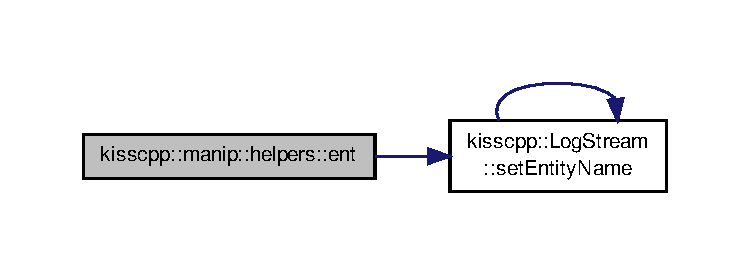
\includegraphics[width=350pt]{namespacekisscpp_1_1manip_1_1helpers_ad663c6941c8fb0937690a6468cc4b350_cgraph}
\end{center}
\end{figure}


\hypertarget{namespacekisscpp_1_1manip_1_1helpers_a3734b7b27eea582e8d748c99ca2da137}{\index{kisscpp\-::manip\-::helpers@{kisscpp\-::manip\-::helpers}!mask@{mask}}
\index{mask@{mask}!kisscpp::manip::helpers@{kisscpp\-::manip\-::helpers}}
\subsubsection[{mask}]{\setlength{\rightskip}{0pt plus 5cm}{\bf Log\-Stream} \& kisscpp\-::manip\-::helpers\-::mask (
\begin{DoxyParamCaption}
\item[{Log\-Stream \&}]{s, }
\item[{uint32\-\_\-t}]{m}
\end{DoxyParamCaption}
)\hspace{0.3cm}{\ttfamily [inline]}}}\label{namespacekisscpp_1_1manip_1_1helpers_a3734b7b27eea582e8d748c99ca2da137}


Here is the call graph for this function\-:
\nopagebreak
\begin{figure}[H]
\begin{center}
\leavevmode
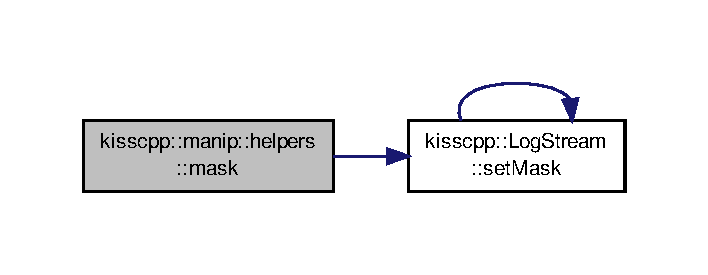
\includegraphics[width=340pt]{namespacekisscpp_1_1manip_1_1helpers_a3734b7b27eea582e8d748c99ca2da137_cgraph}
\end{center}
\end{figure}


\hypertarget{namespacekisscpp_1_1manip_1_1helpers_a97784407250b5ea47c0b20441a7472e5}{\index{kisscpp\-::manip\-::helpers@{kisscpp\-::manip\-::helpers}!source@{source}}
\index{source@{source}!kisscpp::manip::helpers@{kisscpp\-::manip\-::helpers}}
\subsubsection[{source}]{\setlength{\rightskip}{0pt plus 5cm}{\bf Log\-Stream} \& kisscpp\-::manip\-::helpers\-::source (
\begin{DoxyParamCaption}
\item[{Log\-Stream \&}]{s, }
\item[{std\-::string}]{source}
\end{DoxyParamCaption}
)\hspace{0.3cm}{\ttfamily [inline]}}}\label{namespacekisscpp_1_1manip_1_1helpers_a97784407250b5ea47c0b20441a7472e5}


Here is the call graph for this function\-:
\nopagebreak
\begin{figure}[H]
\begin{center}
\leavevmode
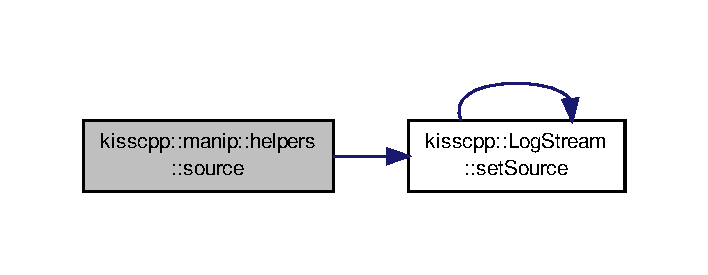
\includegraphics[width=340pt]{namespacekisscpp_1_1manip_1_1helpers_a97784407250b5ea47c0b20441a7472e5_cgraph}
\end{center}
\end{figure}




Here is the caller graph for this function\-:
\nopagebreak
\begin{figure}[H]
\begin{center}
\leavevmode
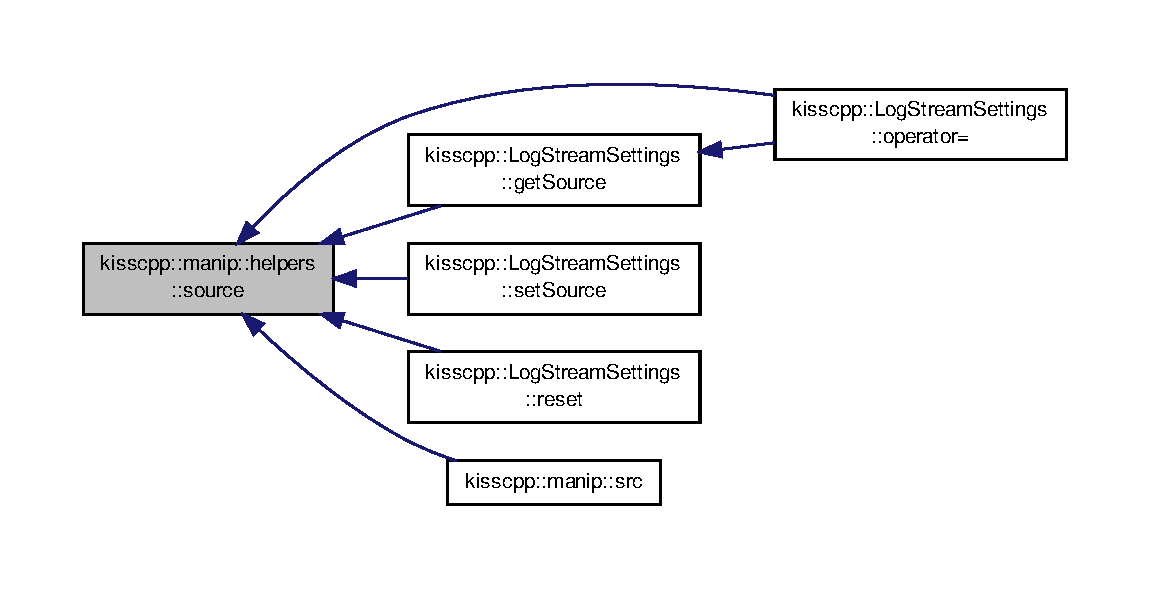
\includegraphics[width=350pt]{namespacekisscpp_1_1manip_1_1helpers_a97784407250b5ea47c0b20441a7472e5_icgraph}
\end{center}
\end{figure}



\chapter{Class Documentation}
\hypertarget{classkisscpp_1_1_base64_bi_coder}{\section{kisscpp\-:\-:Base64\-Bi\-Coder$<$ T $>$ Class Template Reference}
\label{classkisscpp_1_1_base64_bi_coder}\index{kisscpp\-::\-Base64\-Bi\-Coder$<$ T $>$@{kisscpp\-::\-Base64\-Bi\-Coder$<$ T $>$}}
}


{\ttfamily \#include $<$persisted\-\_\-queue.\-hpp$>$}

\subsection*{Public Types}
\begin{DoxyCompactItemize}
\item 
typedef transform\-\_\-width\\*
$<$ binary\-\_\-from\-\_\-base64\\*
$<$ remove\-\_\-whitespace\\*
$<$ std\-::string\-::const\-\_\-iterator $>$ $>$, 8, 6 $>$ \hyperlink{classkisscpp_1_1_base64_bi_coder_a3d4011fcafbdf230c7cc8188714ed499}{Binary\-Type}
\item 
typedef base64\-\_\-from\-\_\-binary\\*
$<$ transform\-\_\-width\\*
$<$ std\-::string\-::const\-\_\-iterator, 6, 8 $>$ $>$ \hyperlink{classkisscpp_1_1_base64_bi_coder_a54d2f4ba00e068e8d4d6fd6497ebf21d}{Base64\-Type}
\end{DoxyCompactItemize}
\subsection*{Public Member Functions}
\begin{DoxyCompactItemize}
\item 
\hyperlink{classkisscpp_1_1_base64_bi_coder_a64d95b2904f11acbddf6d70f19e61b35}{Base64\-Bi\-Coder} ()
\item 
\hyperlink{classkisscpp_1_1_base64_bi_coder_a203c4896daf408dfb45c9d57aea0d959}{$\sim$\-Base64\-Bi\-Coder} ()
\item 
virtual boost\-::shared\-\_\-ptr\\*
$<$ std\-::string $>$ \hyperlink{classkisscpp_1_1_base64_bi_coder_ade4ace8899f97568458a62df0222b32c}{encode} (const boost\-::shared\-\_\-ptr$<$ T $>$ obj2encode)=0
\item 
virtual boost\-::shared\-\_\-ptr$<$ T $>$ \hyperlink{classkisscpp_1_1_base64_bi_coder_a8b3f9d0c6d4d88dded790f7627d0a3ea}{decode} (const std\-::string \&str2decode)=0
\end{DoxyCompactItemize}
\subsection*{Protected Member Functions}
\begin{DoxyCompactItemize}
\item 
boost\-::shared\-\_\-ptr$<$ std\-::string $>$ \hyperlink{classkisscpp_1_1_base64_bi_coder_ab17cf7f1594fa761eca93d6a1ee614ef}{encode\-To\-Base64\-String} (const std\-::string \&s)
\item 
boost\-::shared\-\_\-ptr$<$ std\-::string $>$ \hyperlink{classkisscpp_1_1_base64_bi_coder_af8b91f925c229a0892be4e5d9428fb13}{decode\-From\-Base64} (const std\-::string \&s)
\end{DoxyCompactItemize}


\subsection{Member Typedef Documentation}
\hypertarget{classkisscpp_1_1_base64_bi_coder_a54d2f4ba00e068e8d4d6fd6497ebf21d}{\index{kisscpp\-::\-Base64\-Bi\-Coder@{kisscpp\-::\-Base64\-Bi\-Coder}!Base64\-Type@{Base64\-Type}}
\index{Base64\-Type@{Base64\-Type}!kisscpp::Base64BiCoder@{kisscpp\-::\-Base64\-Bi\-Coder}}
\subsubsection[{Base64\-Type}]{\setlength{\rightskip}{0pt plus 5cm}template$<$class T$>$ typedef base64\-\_\-from\-\_\-binary$<$transform\-\_\-width$<$std\-::string\-::const\-\_\-iterator,6,8$>$ $>$ {\bf kisscpp\-::\-Base64\-Bi\-Coder}$<$ T $>$\-::{\bf Base64\-Type}}}\label{classkisscpp_1_1_base64_bi_coder_a54d2f4ba00e068e8d4d6fd6497ebf21d}
\hypertarget{classkisscpp_1_1_base64_bi_coder_a3d4011fcafbdf230c7cc8188714ed499}{\index{kisscpp\-::\-Base64\-Bi\-Coder@{kisscpp\-::\-Base64\-Bi\-Coder}!Binary\-Type@{Binary\-Type}}
\index{Binary\-Type@{Binary\-Type}!kisscpp::Base64BiCoder@{kisscpp\-::\-Base64\-Bi\-Coder}}
\subsubsection[{Binary\-Type}]{\setlength{\rightskip}{0pt plus 5cm}template$<$class T$>$ typedef transform\-\_\-width$<$ binary\-\_\-from\-\_\-base64$<$remove\-\_\-whitespace$<$std\-::string\-::const\-\_\-iterator$>$ $>$ , 8, 6 $>$ {\bf kisscpp\-::\-Base64\-Bi\-Coder}$<$ T $>$\-::{\bf Binary\-Type}}}\label{classkisscpp_1_1_base64_bi_coder_a3d4011fcafbdf230c7cc8188714ed499}


\subsection{Constructor \& Destructor Documentation}
\hypertarget{classkisscpp_1_1_base64_bi_coder_a64d95b2904f11acbddf6d70f19e61b35}{\index{kisscpp\-::\-Base64\-Bi\-Coder@{kisscpp\-::\-Base64\-Bi\-Coder}!Base64\-Bi\-Coder@{Base64\-Bi\-Coder}}
\index{Base64\-Bi\-Coder@{Base64\-Bi\-Coder}!kisscpp::Base64BiCoder@{kisscpp\-::\-Base64\-Bi\-Coder}}
\subsubsection[{Base64\-Bi\-Coder}]{\setlength{\rightskip}{0pt plus 5cm}template$<$class T$>$ {\bf kisscpp\-::\-Base64\-Bi\-Coder}$<$ T $>$\-::{\bf Base64\-Bi\-Coder} (
\begin{DoxyParamCaption}
{}
\end{DoxyParamCaption}
)\hspace{0.3cm}{\ttfamily [inline]}}}\label{classkisscpp_1_1_base64_bi_coder_a64d95b2904f11acbddf6d70f19e61b35}
\hypertarget{classkisscpp_1_1_base64_bi_coder_a203c4896daf408dfb45c9d57aea0d959}{\index{kisscpp\-::\-Base64\-Bi\-Coder@{kisscpp\-::\-Base64\-Bi\-Coder}!$\sim$\-Base64\-Bi\-Coder@{$\sim$\-Base64\-Bi\-Coder}}
\index{$\sim$\-Base64\-Bi\-Coder@{$\sim$\-Base64\-Bi\-Coder}!kisscpp::Base64BiCoder@{kisscpp\-::\-Base64\-Bi\-Coder}}
\subsubsection[{$\sim$\-Base64\-Bi\-Coder}]{\setlength{\rightskip}{0pt plus 5cm}template$<$class T$>$ {\bf kisscpp\-::\-Base64\-Bi\-Coder}$<$ T $>$\-::$\sim${\bf Base64\-Bi\-Coder} (
\begin{DoxyParamCaption}
{}
\end{DoxyParamCaption}
)\hspace{0.3cm}{\ttfamily [inline]}}}\label{classkisscpp_1_1_base64_bi_coder_a203c4896daf408dfb45c9d57aea0d959}


\subsection{Member Function Documentation}
\hypertarget{classkisscpp_1_1_base64_bi_coder_a8b3f9d0c6d4d88dded790f7627d0a3ea}{\index{kisscpp\-::\-Base64\-Bi\-Coder@{kisscpp\-::\-Base64\-Bi\-Coder}!decode@{decode}}
\index{decode@{decode}!kisscpp::Base64BiCoder@{kisscpp\-::\-Base64\-Bi\-Coder}}
\subsubsection[{decode}]{\setlength{\rightskip}{0pt plus 5cm}template$<$class T$>$ virtual boost\-::shared\-\_\-ptr$<$T$>$ {\bf kisscpp\-::\-Base64\-Bi\-Coder}$<$ T $>$\-::decode (
\begin{DoxyParamCaption}
\item[{const std\-::string \&}]{str2decode}
\end{DoxyParamCaption}
)\hspace{0.3cm}{\ttfamily [pure virtual]}}}\label{classkisscpp_1_1_base64_bi_coder_a8b3f9d0c6d4d88dded790f7627d0a3ea}
\hypertarget{classkisscpp_1_1_base64_bi_coder_af8b91f925c229a0892be4e5d9428fb13}{\index{kisscpp\-::\-Base64\-Bi\-Coder@{kisscpp\-::\-Base64\-Bi\-Coder}!decode\-From\-Base64@{decode\-From\-Base64}}
\index{decode\-From\-Base64@{decode\-From\-Base64}!kisscpp::Base64BiCoder@{kisscpp\-::\-Base64\-Bi\-Coder}}
\subsubsection[{decode\-From\-Base64}]{\setlength{\rightskip}{0pt plus 5cm}template$<$class T$>$ boost\-::shared\-\_\-ptr$<$std\-::string$>$ {\bf kisscpp\-::\-Base64\-Bi\-Coder}$<$ T $>$\-::decode\-From\-Base64 (
\begin{DoxyParamCaption}
\item[{const std\-::string \&}]{s}
\end{DoxyParamCaption}
)\hspace{0.3cm}{\ttfamily [inline]}, {\ttfamily [protected]}}}\label{classkisscpp_1_1_base64_bi_coder_af8b91f925c229a0892be4e5d9428fb13}
\hypertarget{classkisscpp_1_1_base64_bi_coder_ade4ace8899f97568458a62df0222b32c}{\index{kisscpp\-::\-Base64\-Bi\-Coder@{kisscpp\-::\-Base64\-Bi\-Coder}!encode@{encode}}
\index{encode@{encode}!kisscpp::Base64BiCoder@{kisscpp\-::\-Base64\-Bi\-Coder}}
\subsubsection[{encode}]{\setlength{\rightskip}{0pt plus 5cm}template$<$class T$>$ virtual boost\-::shared\-\_\-ptr$<$std\-::string$>$ {\bf kisscpp\-::\-Base64\-Bi\-Coder}$<$ T $>$\-::encode (
\begin{DoxyParamCaption}
\item[{const boost\-::shared\-\_\-ptr$<$ T $>$}]{obj2encode}
\end{DoxyParamCaption}
)\hspace{0.3cm}{\ttfamily [pure virtual]}}}\label{classkisscpp_1_1_base64_bi_coder_ade4ace8899f97568458a62df0222b32c}


Implemented in \hyperlink{classkisscpp_1_1_ptree_base64_bicoder_a7f4bbf8b4b4626fa9228118889fd51d2}{kisscpp\-::\-Ptree\-Base64\-Bicoder}.

\hypertarget{classkisscpp_1_1_base64_bi_coder_ab17cf7f1594fa761eca93d6a1ee614ef}{\index{kisscpp\-::\-Base64\-Bi\-Coder@{kisscpp\-::\-Base64\-Bi\-Coder}!encode\-To\-Base64\-String@{encode\-To\-Base64\-String}}
\index{encode\-To\-Base64\-String@{encode\-To\-Base64\-String}!kisscpp::Base64BiCoder@{kisscpp\-::\-Base64\-Bi\-Coder}}
\subsubsection[{encode\-To\-Base64\-String}]{\setlength{\rightskip}{0pt plus 5cm}template$<$class T$>$ boost\-::shared\-\_\-ptr$<$std\-::string$>$ {\bf kisscpp\-::\-Base64\-Bi\-Coder}$<$ T $>$\-::encode\-To\-Base64\-String (
\begin{DoxyParamCaption}
\item[{const std\-::string \&}]{s}
\end{DoxyParamCaption}
)\hspace{0.3cm}{\ttfamily [inline]}, {\ttfamily [protected]}}}\label{classkisscpp_1_1_base64_bi_coder_ab17cf7f1594fa761eca93d6a1ee614ef}


The documentation for this class was generated from the following file\-:\begin{DoxyCompactItemize}
\item 
\hyperlink{persisted__queue_8hpp}{persisted\-\_\-queue.\-hpp}\end{DoxyCompactItemize}

\hypertarget{classkisscpp_1_1client}{\section{kisscpp\-:\-:client Class Reference}
\label{classkisscpp_1_1client}\index{kisscpp\-::client@{kisscpp\-::client}}
}


{\ttfamily \#include $<$client.\-hpp$>$}

\subsection*{Public Member Functions}
\begin{DoxyCompactItemize}
\item 
\hyperlink{classkisscpp_1_1client_a4cc9b8f3247cb73910d20549014ba859}{client} (\hyperlink{boost__ptree_8hpp_ab36820650b8e0db36402aea80485633c}{Boost\-Ptree} \&\-\_\-request, \hyperlink{boost__ptree_8hpp_ab36820650b8e0db36402aea80485633c}{Boost\-Ptree} \&\-\_\-response, int timeout=10)
\item 
\hyperlink{classkisscpp_1_1client_aa93289217a779bbf3d080035d95e60e1}{$\sim$client} ()
\end{DoxyCompactItemize}


\subsection{Constructor \& Destructor Documentation}
\hypertarget{classkisscpp_1_1client_a4cc9b8f3247cb73910d20549014ba859}{\index{kisscpp\-::client@{kisscpp\-::client}!client@{client}}
\index{client@{client}!kisscpp::client@{kisscpp\-::client}}
\subsubsection[{client}]{\setlength{\rightskip}{0pt plus 5cm}kisscpp\-::client\-::client (
\begin{DoxyParamCaption}
\item[{{\bf Boost\-Ptree} \&}]{\-\_\-request, }
\item[{{\bf Boost\-Ptree} \&}]{\-\_\-response, }
\item[{int}]{timeout = {\ttfamily 10}}
\end{DoxyParamCaption}
)}}\label{classkisscpp_1_1client_a4cc9b8f3247cb73910d20549014ba859}


Here is the call graph for this function\-:
\nopagebreak
\begin{figure}[H]
\begin{center}
\leavevmode
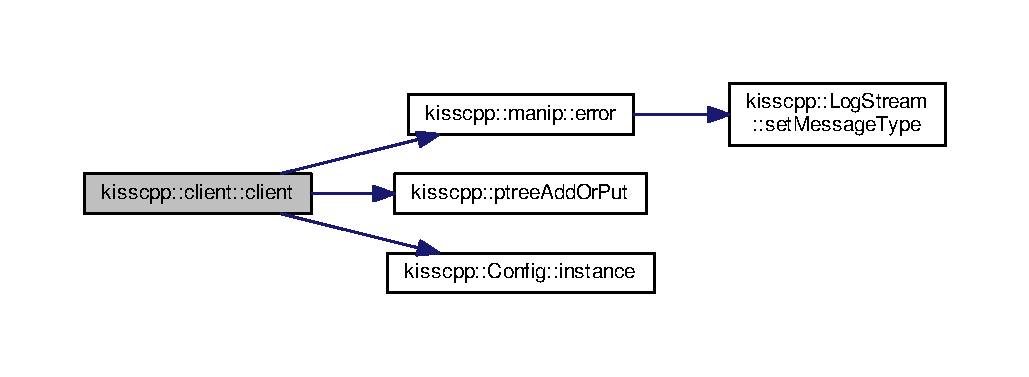
\includegraphics[width=350pt]{classkisscpp_1_1client_a4cc9b8f3247cb73910d20549014ba859_cgraph}
\end{center}
\end{figure}


\hypertarget{classkisscpp_1_1client_aa93289217a779bbf3d080035d95e60e1}{\index{kisscpp\-::client@{kisscpp\-::client}!$\sim$client@{$\sim$client}}
\index{$\sim$client@{$\sim$client}!kisscpp::client@{kisscpp\-::client}}
\subsubsection[{$\sim$client}]{\setlength{\rightskip}{0pt plus 5cm}kisscpp\-::client\-::$\sim$client (
\begin{DoxyParamCaption}
{}
\end{DoxyParamCaption}
)\hspace{0.3cm}{\ttfamily [inline]}}}\label{classkisscpp_1_1client_aa93289217a779bbf3d080035d95e60e1}


The documentation for this class was generated from the following files\-:\begin{DoxyCompactItemize}
\item 
\hyperlink{client_8hpp}{client.\-hpp}\item 
\hyperlink{client_8cpp}{client.\-cpp}\end{DoxyCompactItemize}

\hypertarget{classkisscpp_1_1_config}{\section{kisscpp\-:\-:Config Class Reference}
\label{classkisscpp_1_1_config}\index{kisscpp\-::\-Config@{kisscpp\-::\-Config}}
}


{\ttfamily \#include $<$configuration.\-hpp$>$}

\subsection*{Public Member Functions}
\begin{DoxyCompactItemize}
\item 
void \hyperlink{classkisscpp_1_1_config_a3d46f787270d6aeac04635c04936c404}{initiate} (const std\-::string explicit\-\_\-config\-\_\-path=\char`\"{}\char`\"{})
\item 
\hyperlink{classkisscpp_1_1_config_ae6fd9d0a11285f8dd5658bf07f728e01}{$\sim$\-Config} ()
\item 
\hyperlink{boost__ptree_8hpp_ab36820650b8e0db36402aea80485633c}{Boost\-Ptree} \hyperlink{classkisscpp_1_1_config_a01804b8d8d9c4f3965fd2dd43a46ee83}{get\-\_\-child} (const std\-::string \&s)
\item 
{\footnotesize template$<$typename T $>$ }\\T \hyperlink{classkisscpp_1_1_config_ae237509831f23cd9cbfc67dcd6ed8c9d}{get} (const std\-::string \&s)
\item 
{\footnotesize template$<$typename T $>$ }\\T \hyperlink{classkisscpp_1_1_config_a747baa092e702cb9a42f9c4c74958ddd}{get} (const std\-::string \&s, T default\-\_\-value)
\item 
{\footnotesize template$<$typename T $>$ }\\boost\-::optional$<$ T $>$ \hyperlink{classkisscpp_1_1_config_a0b0267e59a04df930282c0b39e7f79dd}{get\-\_\-optional} (const std\-::string \&s)
\item 
std\-::string \hyperlink{classkisscpp_1_1_config_a5f970e234e909ccb7b18bf4e7705e336}{get\-App\-Id} ()
\item 
std\-::string \hyperlink{classkisscpp_1_1_config_a9a68e47e345ee1fa208397f1c19859f2}{get\-App\-Instance} ()
\item 
bool \hyperlink{classkisscpp_1_1_config_a9b6825f6980d6caa4780567936ce77a6}{is\-Allowed\-Ip} (const std\-::string \&ip\-\_\-address)
\item 
bool \hyperlink{classkisscpp_1_1_config_afb8591ec6e7e7cd86e151f45c7c8ba3b}{is\-Allowed\-Client} (const std\-::string \&app\-\_\-id, const std\-::string \&app\-\_\-instance)
\end{DoxyCompactItemize}
\subsection*{Static Public Member Functions}
\begin{DoxyCompactItemize}
\item 
static \hyperlink{classkisscpp_1_1_config}{Config} $\ast$ \hyperlink{classkisscpp_1_1_config_a235cf3d03c1211faa29efa63556921fc}{instance} (const std\-::string app\-\_\-id=\char`\"{}kisscpp\-\_\-application\char`\"{}, const std\-::string app\-\_\-instance=\char`\"{}0\char`\"{}, const std\-::string explicit\-\_\-config\-\_\-path=\char`\"{}\char`\"{})
\end{DoxyCompactItemize}


\subsection{Constructor \& Destructor Documentation}
\hypertarget{classkisscpp_1_1_config_ae6fd9d0a11285f8dd5658bf07f728e01}{\index{kisscpp\-::\-Config@{kisscpp\-::\-Config}!$\sim$\-Config@{$\sim$\-Config}}
\index{$\sim$\-Config@{$\sim$\-Config}!kisscpp::Config@{kisscpp\-::\-Config}}
\subsubsection[{$\sim$\-Config}]{\setlength{\rightskip}{0pt plus 5cm}kisscpp\-::\-Config\-::$\sim$\-Config (
\begin{DoxyParamCaption}
{}
\end{DoxyParamCaption}
)\hspace{0.3cm}{\ttfamily [inline]}}}\label{classkisscpp_1_1_config_ae6fd9d0a11285f8dd5658bf07f728e01}


\subsection{Member Function Documentation}
\hypertarget{classkisscpp_1_1_config_ae237509831f23cd9cbfc67dcd6ed8c9d}{\index{kisscpp\-::\-Config@{kisscpp\-::\-Config}!get@{get}}
\index{get@{get}!kisscpp::Config@{kisscpp\-::\-Config}}
\subsubsection[{get}]{\setlength{\rightskip}{0pt plus 5cm}template$<$typename T $>$ T kisscpp\-::\-Config\-::get (
\begin{DoxyParamCaption}
\item[{const std\-::string \&}]{s}
\end{DoxyParamCaption}
)\hspace{0.3cm}{\ttfamily [inline]}}}\label{classkisscpp_1_1_config_ae237509831f23cd9cbfc67dcd6ed8c9d}


Here is the caller graph for this function\-:
\nopagebreak
\begin{figure}[H]
\begin{center}
\leavevmode
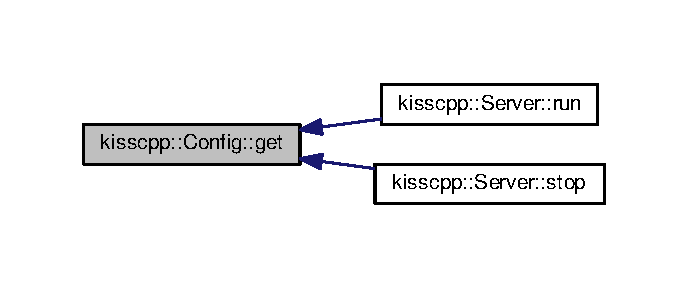
\includegraphics[width=330pt]{classkisscpp_1_1_config_ae237509831f23cd9cbfc67dcd6ed8c9d_icgraph}
\end{center}
\end{figure}


\hypertarget{classkisscpp_1_1_config_a747baa092e702cb9a42f9c4c74958ddd}{\index{kisscpp\-::\-Config@{kisscpp\-::\-Config}!get@{get}}
\index{get@{get}!kisscpp::Config@{kisscpp\-::\-Config}}
\subsubsection[{get}]{\setlength{\rightskip}{0pt plus 5cm}template$<$typename T $>$ T kisscpp\-::\-Config\-::get (
\begin{DoxyParamCaption}
\item[{const std\-::string \&}]{s, }
\item[{T}]{default\-\_\-value}
\end{DoxyParamCaption}
)\hspace{0.3cm}{\ttfamily [inline]}}}\label{classkisscpp_1_1_config_a747baa092e702cb9a42f9c4c74958ddd}
\hypertarget{classkisscpp_1_1_config_a01804b8d8d9c4f3965fd2dd43a46ee83}{\index{kisscpp\-::\-Config@{kisscpp\-::\-Config}!get\-\_\-child@{get\-\_\-child}}
\index{get\-\_\-child@{get\-\_\-child}!kisscpp::Config@{kisscpp\-::\-Config}}
\subsubsection[{get\-\_\-child}]{\setlength{\rightskip}{0pt plus 5cm}{\bf Boost\-Ptree} kisscpp\-::\-Config\-::get\-\_\-child (
\begin{DoxyParamCaption}
\item[{const std\-::string \&}]{s}
\end{DoxyParamCaption}
)\hspace{0.3cm}{\ttfamily [inline]}}}\label{classkisscpp_1_1_config_a01804b8d8d9c4f3965fd2dd43a46ee83}
\hypertarget{classkisscpp_1_1_config_a0b0267e59a04df930282c0b39e7f79dd}{\index{kisscpp\-::\-Config@{kisscpp\-::\-Config}!get\-\_\-optional@{get\-\_\-optional}}
\index{get\-\_\-optional@{get\-\_\-optional}!kisscpp::Config@{kisscpp\-::\-Config}}
\subsubsection[{get\-\_\-optional}]{\setlength{\rightskip}{0pt plus 5cm}template$<$typename T $>$ boost\-::optional$<$T$>$ kisscpp\-::\-Config\-::get\-\_\-optional (
\begin{DoxyParamCaption}
\item[{const std\-::string \&}]{s}
\end{DoxyParamCaption}
)\hspace{0.3cm}{\ttfamily [inline]}}}\label{classkisscpp_1_1_config_a0b0267e59a04df930282c0b39e7f79dd}
\hypertarget{classkisscpp_1_1_config_a5f970e234e909ccb7b18bf4e7705e336}{\index{kisscpp\-::\-Config@{kisscpp\-::\-Config}!get\-App\-Id@{get\-App\-Id}}
\index{get\-App\-Id@{get\-App\-Id}!kisscpp::Config@{kisscpp\-::\-Config}}
\subsubsection[{get\-App\-Id}]{\setlength{\rightskip}{0pt plus 5cm}std\-::string kisscpp\-::\-Config\-::get\-App\-Id (
\begin{DoxyParamCaption}
{}
\end{DoxyParamCaption}
)\hspace{0.3cm}{\ttfamily [inline]}}}\label{classkisscpp_1_1_config_a5f970e234e909ccb7b18bf4e7705e336}


Here is the caller graph for this function\-:
\nopagebreak
\begin{figure}[H]
\begin{center}
\leavevmode
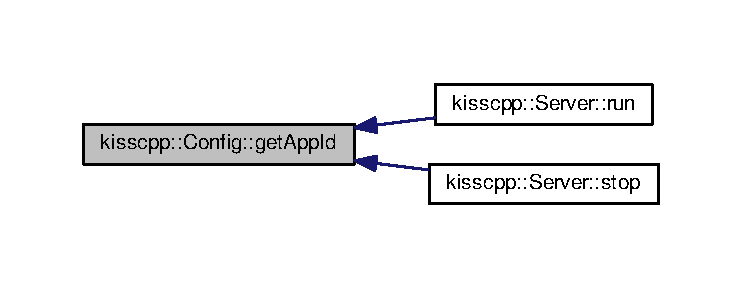
\includegraphics[width=350pt]{classkisscpp_1_1_config_a5f970e234e909ccb7b18bf4e7705e336_icgraph}
\end{center}
\end{figure}


\hypertarget{classkisscpp_1_1_config_a9a68e47e345ee1fa208397f1c19859f2}{\index{kisscpp\-::\-Config@{kisscpp\-::\-Config}!get\-App\-Instance@{get\-App\-Instance}}
\index{get\-App\-Instance@{get\-App\-Instance}!kisscpp::Config@{kisscpp\-::\-Config}}
\subsubsection[{get\-App\-Instance}]{\setlength{\rightskip}{0pt plus 5cm}std\-::string kisscpp\-::\-Config\-::get\-App\-Instance (
\begin{DoxyParamCaption}
{}
\end{DoxyParamCaption}
)\hspace{0.3cm}{\ttfamily [inline]}}}\label{classkisscpp_1_1_config_a9a68e47e345ee1fa208397f1c19859f2}


Here is the caller graph for this function\-:
\nopagebreak
\begin{figure}[H]
\begin{center}
\leavevmode
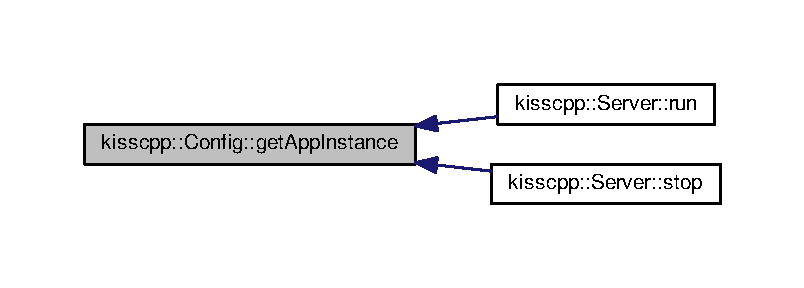
\includegraphics[width=350pt]{classkisscpp_1_1_config_a9a68e47e345ee1fa208397f1c19859f2_icgraph}
\end{center}
\end{figure}


\hypertarget{classkisscpp_1_1_config_a3d46f787270d6aeac04635c04936c404}{\index{kisscpp\-::\-Config@{kisscpp\-::\-Config}!initiate@{initiate}}
\index{initiate@{initiate}!kisscpp::Config@{kisscpp\-::\-Config}}
\subsubsection[{initiate}]{\setlength{\rightskip}{0pt plus 5cm}void kisscpp\-::\-Config\-::initiate (
\begin{DoxyParamCaption}
\item[{const std\-::string}]{explicit\-\_\-config\-\_\-path = {\ttfamily \char`\"{}\char`\"{}}}
\end{DoxyParamCaption}
)}}\label{classkisscpp_1_1_config_a3d46f787270d6aeac04635c04936c404}
\hypertarget{classkisscpp_1_1_config_a235cf3d03c1211faa29efa63556921fc}{\index{kisscpp\-::\-Config@{kisscpp\-::\-Config}!instance@{instance}}
\index{instance@{instance}!kisscpp::Config@{kisscpp\-::\-Config}}
\subsubsection[{instance}]{\setlength{\rightskip}{0pt plus 5cm}{\bf Config} $\ast$ kisscpp\-::\-Config\-::instance (
\begin{DoxyParamCaption}
\item[{const std\-::string}]{app\-\_\-id = {\ttfamily \char`\"{}kisscpp\-\_\-application\char`\"{}}, }
\item[{const std\-::string}]{app\-\_\-instance = {\ttfamily \char`\"{}0\char`\"{}}, }
\item[{const std\-::string}]{explicit\-\_\-config\-\_\-path = {\ttfamily \char`\"{}\char`\"{}}}
\end{DoxyParamCaption}
)\hspace{0.3cm}{\ttfamily [static]}}}\label{classkisscpp_1_1_config_a235cf3d03c1211faa29efa63556921fc}


Here is the caller graph for this function\-:
\nopagebreak
\begin{figure}[H]
\begin{center}
\leavevmode
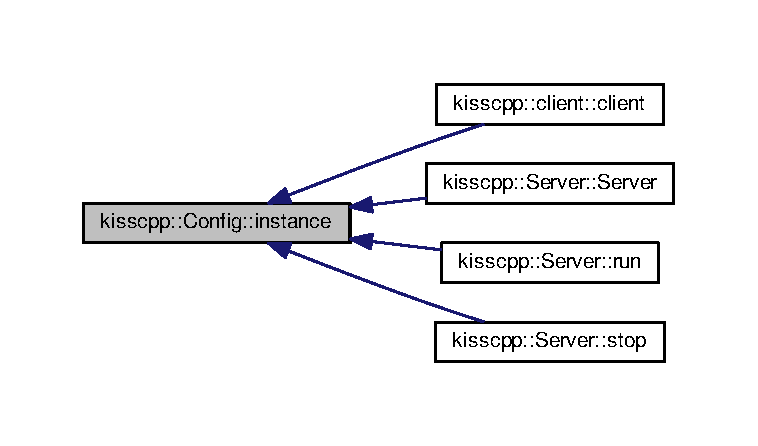
\includegraphics[width=350pt]{classkisscpp_1_1_config_a235cf3d03c1211faa29efa63556921fc_icgraph}
\end{center}
\end{figure}


\hypertarget{classkisscpp_1_1_config_afb8591ec6e7e7cd86e151f45c7c8ba3b}{\index{kisscpp\-::\-Config@{kisscpp\-::\-Config}!is\-Allowed\-Client@{is\-Allowed\-Client}}
\index{is\-Allowed\-Client@{is\-Allowed\-Client}!kisscpp::Config@{kisscpp\-::\-Config}}
\subsubsection[{is\-Allowed\-Client}]{\setlength{\rightskip}{0pt plus 5cm}bool kisscpp\-::\-Config\-::is\-Allowed\-Client (
\begin{DoxyParamCaption}
\item[{const std\-::string \&}]{app\-\_\-id, }
\item[{const std\-::string \&}]{app\-\_\-instance}
\end{DoxyParamCaption}
)}}\label{classkisscpp_1_1_config_afb8591ec6e7e7cd86e151f45c7c8ba3b}
\hypertarget{classkisscpp_1_1_config_a9b6825f6980d6caa4780567936ce77a6}{\index{kisscpp\-::\-Config@{kisscpp\-::\-Config}!is\-Allowed\-Ip@{is\-Allowed\-Ip}}
\index{is\-Allowed\-Ip@{is\-Allowed\-Ip}!kisscpp::Config@{kisscpp\-::\-Config}}
\subsubsection[{is\-Allowed\-Ip}]{\setlength{\rightskip}{0pt plus 5cm}bool kisscpp\-::\-Config\-::is\-Allowed\-Ip (
\begin{DoxyParamCaption}
\item[{const std\-::string \&}]{ip\-\_\-address}
\end{DoxyParamCaption}
)}}\label{classkisscpp_1_1_config_a9b6825f6980d6caa4780567936ce77a6}


The documentation for this class was generated from the following files\-:\begin{DoxyCompactItemize}
\item 
\hyperlink{configuration_8hpp}{configuration.\-hpp}\item 
\hyperlink{configuration_8cpp}{configuration.\-cpp}\end{DoxyCompactItemize}

\hypertarget{classkisscpp_1_1_connection}{\section{kisscpp\-:\-:Connection Class Reference}
\label{classkisscpp_1_1_connection}\index{kisscpp\-::\-Connection@{kisscpp\-::\-Connection}}
}


{\ttfamily \#include $<$connection.\-hpp$>$}



Inheritance diagram for kisscpp\-:\-:Connection\-:\nopagebreak
\begin{figure}[H]
\begin{center}
\leavevmode
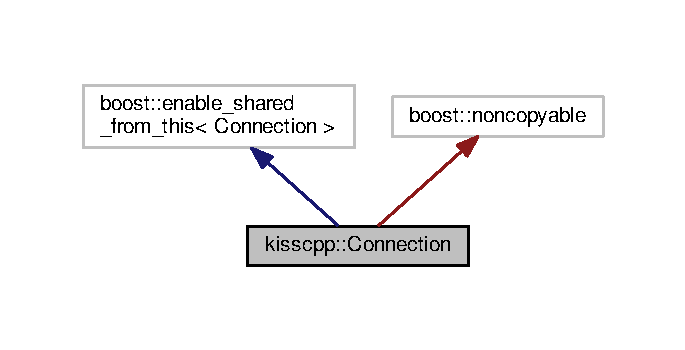
\includegraphics[width=329pt]{classkisscpp_1_1_connection__inherit__graph}
\end{center}
\end{figure}


Collaboration diagram for kisscpp\-:\-:Connection\-:\nopagebreak
\begin{figure}[H]
\begin{center}
\leavevmode
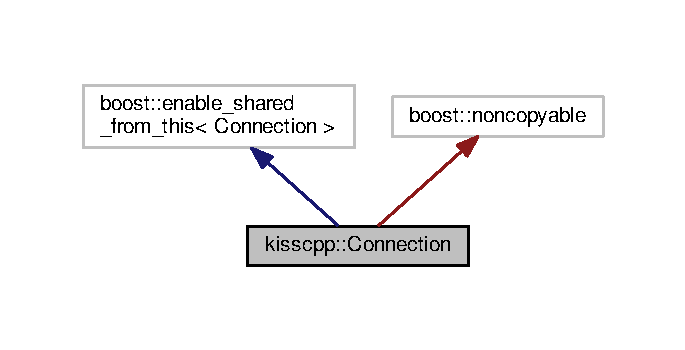
\includegraphics[width=329pt]{classkisscpp_1_1_connection__coll__graph}
\end{center}
\end{figure}
\subsection*{Public Member Functions}
\begin{DoxyCompactItemize}
\item 
\hyperlink{classkisscpp_1_1_connection_aa1cd7b458cc101092c9a83c4618e6f4e}{Connection} (boost\-::asio\-::io\-\_\-service \&io\-\_\-service, \hyperlink{classkisscpp_1_1_request_router}{Request\-Router} \&handler)
\item 
\hyperlink{classkisscpp_1_1_connection_acdc21c339ec95978cf74f38c395430dd}{$\sim$\-Connection} ()
\item 
boost\-::asio\-::ip\-::tcp\-::socket \& \hyperlink{classkisscpp_1_1_connection_af8fa26370281f97e44bc05a669c7f040}{socket} ()
\item 
void \hyperlink{classkisscpp_1_1_connection_aaad88f72fad4844f03e5dd55320caeae}{start} ()
\end{DoxyCompactItemize}


\subsection{Constructor \& Destructor Documentation}
\hypertarget{classkisscpp_1_1_connection_aa1cd7b458cc101092c9a83c4618e6f4e}{\index{kisscpp\-::\-Connection@{kisscpp\-::\-Connection}!Connection@{Connection}}
\index{Connection@{Connection}!kisscpp::Connection@{kisscpp\-::\-Connection}}
\subsubsection[{Connection}]{\setlength{\rightskip}{0pt plus 5cm}kisscpp\-::\-Connection\-::\-Connection (
\begin{DoxyParamCaption}
\item[{boost\-::asio\-::io\-\_\-service \&}]{io\-\_\-service, }
\item[{{\bf Request\-Router} \&}]{handler}
\end{DoxyParamCaption}
)\hspace{0.3cm}{\ttfamily [explicit]}}}\label{classkisscpp_1_1_connection_aa1cd7b458cc101092c9a83c4618e6f4e}
\hypertarget{classkisscpp_1_1_connection_acdc21c339ec95978cf74f38c395430dd}{\index{kisscpp\-::\-Connection@{kisscpp\-::\-Connection}!$\sim$\-Connection@{$\sim$\-Connection}}
\index{$\sim$\-Connection@{$\sim$\-Connection}!kisscpp::Connection@{kisscpp\-::\-Connection}}
\subsubsection[{$\sim$\-Connection}]{\setlength{\rightskip}{0pt plus 5cm}kisscpp\-::\-Connection\-::$\sim$\-Connection (
\begin{DoxyParamCaption}
{}
\end{DoxyParamCaption}
)\hspace{0.3cm}{\ttfamily [inline]}}}\label{classkisscpp_1_1_connection_acdc21c339ec95978cf74f38c395430dd}


\subsection{Member Function Documentation}
\hypertarget{classkisscpp_1_1_connection_af8fa26370281f97e44bc05a669c7f040}{\index{kisscpp\-::\-Connection@{kisscpp\-::\-Connection}!socket@{socket}}
\index{socket@{socket}!kisscpp::Connection@{kisscpp\-::\-Connection}}
\subsubsection[{socket}]{\setlength{\rightskip}{0pt plus 5cm}boost\-::asio\-::ip\-::tcp\-::socket \& kisscpp\-::\-Connection\-::socket (
\begin{DoxyParamCaption}
{}
\end{DoxyParamCaption}
)}}\label{classkisscpp_1_1_connection_af8fa26370281f97e44bc05a669c7f040}
\hypertarget{classkisscpp_1_1_connection_aaad88f72fad4844f03e5dd55320caeae}{\index{kisscpp\-::\-Connection@{kisscpp\-::\-Connection}!start@{start}}
\index{start@{start}!kisscpp::Connection@{kisscpp\-::\-Connection}}
\subsubsection[{start}]{\setlength{\rightskip}{0pt plus 5cm}void kisscpp\-::\-Connection\-::start (
\begin{DoxyParamCaption}
{}
\end{DoxyParamCaption}
)}}\label{classkisscpp_1_1_connection_aaad88f72fad4844f03e5dd55320caeae}


Here is the call graph for this function\-:\nopagebreak
\begin{figure}[H]
\begin{center}
\leavevmode
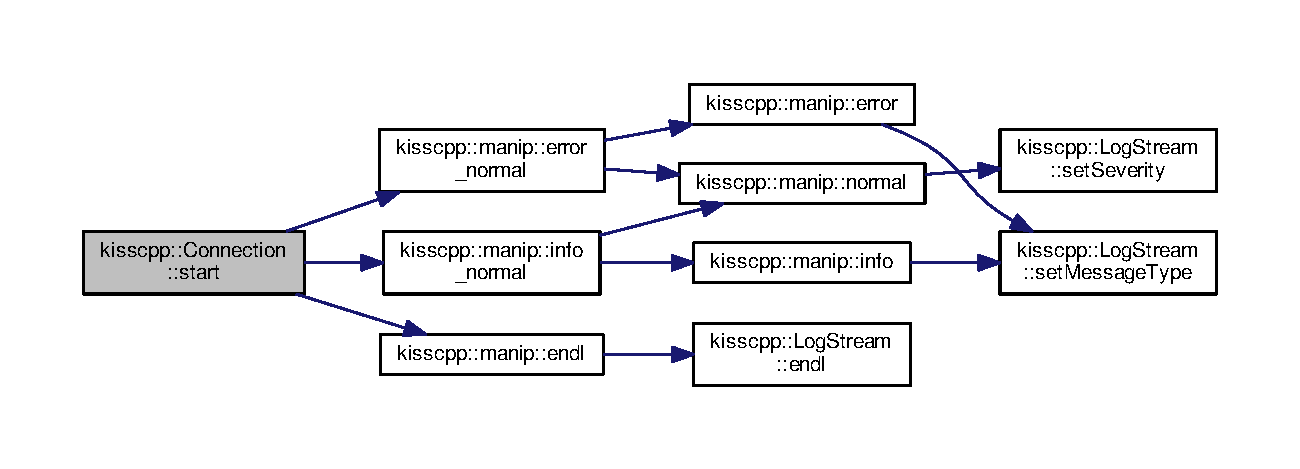
\includegraphics[width=350pt]{classkisscpp_1_1_connection_aaad88f72fad4844f03e5dd55320caeae_cgraph}
\end{center}
\end{figure}




The documentation for this class was generated from the following files\-:\begin{DoxyCompactItemize}
\item 
\hyperlink{connection_8hpp}{connection.\-hpp}\item 
\hyperlink{connection_8cpp}{connection.\-cpp}\end{DoxyCompactItemize}

\hypertarget{classkisscpp_1_1_error_reporter}{\section{kisscpp\-:\-:Error\-Reporter Class Reference}
\label{classkisscpp_1_1_error_reporter}\index{kisscpp\-::\-Error\-Reporter@{kisscpp\-::\-Error\-Reporter}}
}


{\ttfamily \#include $<$standard\-\_\-handlers.\-hpp$>$}



Inheritance diagram for kisscpp\-:\-:Error\-Reporter\-:\nopagebreak
\begin{figure}[H]
\begin{center}
\leavevmode
\includegraphics[width=206pt]{classkisscpp_1_1_error_reporter__inherit__graph}
\end{center}
\end{figure}


Collaboration diagram for kisscpp\-:\-:Error\-Reporter\-:\nopagebreak
\begin{figure}[H]
\begin{center}
\leavevmode
\includegraphics[width=206pt]{classkisscpp_1_1_error_reporter__coll__graph}
\end{center}
\end{figure}
\subsection*{Public Member Functions}
\begin{DoxyCompactItemize}
\item 
\hyperlink{classkisscpp_1_1_error_reporter_ae772ce0549cded2acb8909b420c4b6d7}{Error\-Reporter} ()
\item 
\hyperlink{classkisscpp_1_1_error_reporter_a497e32bd73503b28283b3e64fd0ac45c}{$\sim$\-Error\-Reporter} ()
\item 
void \hyperlink{classkisscpp_1_1_error_reporter_a7afc458c0a447f93f138f006acb57117}{run} (const \hyperlink{boost__ptree_8hpp_ab36820650b8e0db36402aea80485633c}{Boost\-Ptree} \&request, \hyperlink{boost__ptree_8hpp_ab36820650b8e0db36402aea80485633c}{Boost\-Ptree} \&response)
\end{DoxyCompactItemize}


\subsection{Constructor \& Destructor Documentation}
\hypertarget{classkisscpp_1_1_error_reporter_ae772ce0549cded2acb8909b420c4b6d7}{\index{kisscpp\-::\-Error\-Reporter@{kisscpp\-::\-Error\-Reporter}!Error\-Reporter@{Error\-Reporter}}
\index{Error\-Reporter@{Error\-Reporter}!kisscpp::ErrorReporter@{kisscpp\-::\-Error\-Reporter}}
\subsubsection[{Error\-Reporter}]{\setlength{\rightskip}{0pt plus 5cm}kisscpp\-::\-Error\-Reporter\-::\-Error\-Reporter (
\begin{DoxyParamCaption}
{}
\end{DoxyParamCaption}
)\hspace{0.3cm}{\ttfamily [inline]}}}\label{classkisscpp_1_1_error_reporter_ae772ce0549cded2acb8909b420c4b6d7}
\hypertarget{classkisscpp_1_1_error_reporter_a497e32bd73503b28283b3e64fd0ac45c}{\index{kisscpp\-::\-Error\-Reporter@{kisscpp\-::\-Error\-Reporter}!$\sim$\-Error\-Reporter@{$\sim$\-Error\-Reporter}}
\index{$\sim$\-Error\-Reporter@{$\sim$\-Error\-Reporter}!kisscpp::ErrorReporter@{kisscpp\-::\-Error\-Reporter}}
\subsubsection[{$\sim$\-Error\-Reporter}]{\setlength{\rightskip}{0pt plus 5cm}kisscpp\-::\-Error\-Reporter\-::$\sim$\-Error\-Reporter (
\begin{DoxyParamCaption}
{}
\end{DoxyParamCaption}
)\hspace{0.3cm}{\ttfamily [inline]}}}\label{classkisscpp_1_1_error_reporter_a497e32bd73503b28283b3e64fd0ac45c}


\subsection{Member Function Documentation}
\hypertarget{classkisscpp_1_1_error_reporter_a7afc458c0a447f93f138f006acb57117}{\index{kisscpp\-::\-Error\-Reporter@{kisscpp\-::\-Error\-Reporter}!run@{run}}
\index{run@{run}!kisscpp::ErrorReporter@{kisscpp\-::\-Error\-Reporter}}
\subsubsection[{run}]{\setlength{\rightskip}{0pt plus 5cm}void kisscpp\-::\-Error\-Reporter\-::run (
\begin{DoxyParamCaption}
\item[{const {\bf Boost\-Ptree} \&}]{request, }
\item[{{\bf Boost\-Ptree} \&}]{response}
\end{DoxyParamCaption}
)\hspace{0.3cm}{\ttfamily [virtual]}}}\label{classkisscpp_1_1_error_reporter_a7afc458c0a447f93f138f006acb57117}


Implements \hyperlink{classkisscpp_1_1_request_handler_a3606f772c07297826847a8e36226cdaa}{kisscpp\-::\-Request\-Handler}.



Here is the call graph for this function\-:\nopagebreak
\begin{figure}[H]
\begin{center}
\leavevmode
\includegraphics[width=350pt]{classkisscpp_1_1_error_reporter_a7afc458c0a447f93f138f006acb57117_cgraph}
\end{center}
\end{figure}




The documentation for this class was generated from the following files\-:\begin{DoxyCompactItemize}
\item 
\hyperlink{standard__handlers_8hpp}{standard\-\_\-handlers.\-hpp}\item 
\hyperlink{standard__handlers_8cpp}{standard\-\_\-handlers.\-cpp}\end{DoxyCompactItemize}

\hypertarget{classkisscpp_1_1_error_state}{\section{kisscpp\-:\-:Error\-State Class Reference}
\label{classkisscpp_1_1_error_state}\index{kisscpp\-::\-Error\-State@{kisscpp\-::\-Error\-State}}
}


{\ttfamily \#include $<$errorstate.\-hpp$>$}

\subsection*{Public Member Functions}
\begin{DoxyCompactItemize}
\item 
\hyperlink{classkisscpp_1_1_error_state_a0b9109ca4cb0c58114b7b0e32638f18c}{Error\-State} (const std\-::string \&\-\_\-id)
\item 
\hyperlink{classkisscpp_1_1_error_state_a75f55fa61878bb008abd861012b88662}{$\sim$\-Error\-State} ()
\item 
void \hyperlink{classkisscpp_1_1_error_state_adba9283ecd7976c57ef48d438da86778}{set} ()
\item 
void \hyperlink{classkisscpp_1_1_error_state_a2d6939dda90115b7f93a03595296e49b}{clear} (const unsigned int \&amount=1)
\item 
void \hyperlink{classkisscpp_1_1_error_state_aa9da790733f2f6963a5b6ca1167d137b}{clear\-\_\-all} ()
\item 
unsigned int \hyperlink{classkisscpp_1_1_error_state_a211a4d0740010a7aa7c78b8514bc6969}{get\-Set\-Count} ()
\item 
bool \hyperlink{classkisscpp_1_1_error_state_a79c9043eb6c04a10e7c4b86888697ce8}{is\-Set} ()
\end{DoxyCompactItemize}


\subsection{Constructor \& Destructor Documentation}
\hypertarget{classkisscpp_1_1_error_state_a0b9109ca4cb0c58114b7b0e32638f18c}{\index{kisscpp\-::\-Error\-State@{kisscpp\-::\-Error\-State}!Error\-State@{Error\-State}}
\index{Error\-State@{Error\-State}!kisscpp::ErrorState@{kisscpp\-::\-Error\-State}}
\subsubsection[{Error\-State}]{\setlength{\rightskip}{0pt plus 5cm}kisscpp\-::\-Error\-State\-::\-Error\-State (
\begin{DoxyParamCaption}
\item[{const std\-::string \&}]{\-\_\-id}
\end{DoxyParamCaption}
)\hspace{0.3cm}{\ttfamily [inline]}}}\label{classkisscpp_1_1_error_state_a0b9109ca4cb0c58114b7b0e32638f18c}
\hypertarget{classkisscpp_1_1_error_state_a75f55fa61878bb008abd861012b88662}{\index{kisscpp\-::\-Error\-State@{kisscpp\-::\-Error\-State}!$\sim$\-Error\-State@{$\sim$\-Error\-State}}
\index{$\sim$\-Error\-State@{$\sim$\-Error\-State}!kisscpp::ErrorState@{kisscpp\-::\-Error\-State}}
\subsubsection[{$\sim$\-Error\-State}]{\setlength{\rightskip}{0pt plus 5cm}kisscpp\-::\-Error\-State\-::$\sim$\-Error\-State (
\begin{DoxyParamCaption}
{}
\end{DoxyParamCaption}
)\hspace{0.3cm}{\ttfamily [inline]}}}\label{classkisscpp_1_1_error_state_a75f55fa61878bb008abd861012b88662}


\subsection{Member Function Documentation}
\hypertarget{classkisscpp_1_1_error_state_a2d6939dda90115b7f93a03595296e49b}{\index{kisscpp\-::\-Error\-State@{kisscpp\-::\-Error\-State}!clear@{clear}}
\index{clear@{clear}!kisscpp::ErrorState@{kisscpp\-::\-Error\-State}}
\subsubsection[{clear}]{\setlength{\rightskip}{0pt plus 5cm}void kisscpp\-::\-Error\-State\-::clear (
\begin{DoxyParamCaption}
\item[{const unsigned int \&}]{amount = {\ttfamily 1}}
\end{DoxyParamCaption}
)\hspace{0.3cm}{\ttfamily [inline]}}}\label{classkisscpp_1_1_error_state_a2d6939dda90115b7f93a03595296e49b}
\hypertarget{classkisscpp_1_1_error_state_aa9da790733f2f6963a5b6ca1167d137b}{\index{kisscpp\-::\-Error\-State@{kisscpp\-::\-Error\-State}!clear\-\_\-all@{clear\-\_\-all}}
\index{clear\-\_\-all@{clear\-\_\-all}!kisscpp::ErrorState@{kisscpp\-::\-Error\-State}}
\subsubsection[{clear\-\_\-all}]{\setlength{\rightskip}{0pt plus 5cm}void kisscpp\-::\-Error\-State\-::clear\-\_\-all (
\begin{DoxyParamCaption}
{}
\end{DoxyParamCaption}
)\hspace{0.3cm}{\ttfamily [inline]}}}\label{classkisscpp_1_1_error_state_aa9da790733f2f6963a5b6ca1167d137b}
\hypertarget{classkisscpp_1_1_error_state_a211a4d0740010a7aa7c78b8514bc6969}{\index{kisscpp\-::\-Error\-State@{kisscpp\-::\-Error\-State}!get\-Set\-Count@{get\-Set\-Count}}
\index{get\-Set\-Count@{get\-Set\-Count}!kisscpp::ErrorState@{kisscpp\-::\-Error\-State}}
\subsubsection[{get\-Set\-Count}]{\setlength{\rightskip}{0pt plus 5cm}unsigned int kisscpp\-::\-Error\-State\-::get\-Set\-Count (
\begin{DoxyParamCaption}
{}
\end{DoxyParamCaption}
)\hspace{0.3cm}{\ttfamily [inline]}}}\label{classkisscpp_1_1_error_state_a211a4d0740010a7aa7c78b8514bc6969}
\hypertarget{classkisscpp_1_1_error_state_a79c9043eb6c04a10e7c4b86888697ce8}{\index{kisscpp\-::\-Error\-State@{kisscpp\-::\-Error\-State}!is\-Set@{is\-Set}}
\index{is\-Set@{is\-Set}!kisscpp::ErrorState@{kisscpp\-::\-Error\-State}}
\subsubsection[{is\-Set}]{\setlength{\rightskip}{0pt plus 5cm}bool kisscpp\-::\-Error\-State\-::is\-Set (
\begin{DoxyParamCaption}
{}
\end{DoxyParamCaption}
)\hspace{0.3cm}{\ttfamily [inline]}}}\label{classkisscpp_1_1_error_state_a79c9043eb6c04a10e7c4b86888697ce8}
\hypertarget{classkisscpp_1_1_error_state_adba9283ecd7976c57ef48d438da86778}{\index{kisscpp\-::\-Error\-State@{kisscpp\-::\-Error\-State}!set@{set}}
\index{set@{set}!kisscpp::ErrorState@{kisscpp\-::\-Error\-State}}
\subsubsection[{set}]{\setlength{\rightskip}{0pt plus 5cm}void kisscpp\-::\-Error\-State\-::set (
\begin{DoxyParamCaption}
{}
\end{DoxyParamCaption}
)\hspace{0.3cm}{\ttfamily [inline]}}}\label{classkisscpp_1_1_error_state_adba9283ecd7976c57ef48d438da86778}


The documentation for this class was generated from the following file\-:\begin{DoxyCompactItemize}
\item 
\hyperlink{errorstate_8hpp}{errorstate.\-hpp}\end{DoxyCompactItemize}

\hypertarget{classkisscpp_1_1_error_state_list}{\section{kisscpp\-:\-:Error\-State\-List Class Reference}
\label{classkisscpp_1_1_error_state_list}\index{kisscpp\-::\-Error\-State\-List@{kisscpp\-::\-Error\-State\-List}}
}


{\ttfamily \#include $<$errorstate.\-hpp$>$}

\subsection*{Public Member Functions}
\begin{DoxyCompactItemize}
\item 
\hyperlink{classkisscpp_1_1_error_state_list_a0c53a01c63906189fad454dd5e217181}{$\sim$\-Error\-State\-List} ()
\item 
void \hyperlink{classkisscpp_1_1_error_state_list_ae3998a49baee5f0aa709dbd6bb9e0397}{set} (const std\-::string \&id)
\item 
void \hyperlink{classkisscpp_1_1_error_state_list_a848953f011b5acc35538bb82f35ef67f}{clear} (const std\-::string \&id, const unsigned int \&amount=1)
\item 
void \hyperlink{classkisscpp_1_1_error_state_list_a4cf6d39a68e8dbbae8111ea383aaf14a}{clear\-\_\-all} (const std\-::string \&id)
\item 
\hyperlink{namespacekisscpp_a52b7a11959a119c1da931042d7751db0}{Shared\-Error\-List\-Map} \hyperlink{classkisscpp_1_1_error_state_list_af51ba7384104a15f7809f62da9c5447d}{get\-States} ()
\end{DoxyCompactItemize}
\subsection*{Static Public Member Functions}
\begin{DoxyCompactItemize}
\item 
static \hyperlink{classkisscpp_1_1_error_state_list}{Error\-State\-List} $\ast$ \hyperlink{classkisscpp_1_1_error_state_list_a20309374dc63ffee8aebeb986340dfba}{instance} ()
\end{DoxyCompactItemize}


\subsection{Constructor \& Destructor Documentation}
\hypertarget{classkisscpp_1_1_error_state_list_a0c53a01c63906189fad454dd5e217181}{\index{kisscpp\-::\-Error\-State\-List@{kisscpp\-::\-Error\-State\-List}!$\sim$\-Error\-State\-List@{$\sim$\-Error\-State\-List}}
\index{$\sim$\-Error\-State\-List@{$\sim$\-Error\-State\-List}!kisscpp::ErrorStateList@{kisscpp\-::\-Error\-State\-List}}
\subsubsection[{$\sim$\-Error\-State\-List}]{\setlength{\rightskip}{0pt plus 5cm}kisscpp\-::\-Error\-State\-List\-::$\sim$\-Error\-State\-List (
\begin{DoxyParamCaption}
{}
\end{DoxyParamCaption}
)\hspace{0.3cm}{\ttfamily [inline]}}}\label{classkisscpp_1_1_error_state_list_a0c53a01c63906189fad454dd5e217181}


\subsection{Member Function Documentation}
\hypertarget{classkisscpp_1_1_error_state_list_a848953f011b5acc35538bb82f35ef67f}{\index{kisscpp\-::\-Error\-State\-List@{kisscpp\-::\-Error\-State\-List}!clear@{clear}}
\index{clear@{clear}!kisscpp::ErrorStateList@{kisscpp\-::\-Error\-State\-List}}
\subsubsection[{clear}]{\setlength{\rightskip}{0pt plus 5cm}void kisscpp\-::\-Error\-State\-List\-::clear (
\begin{DoxyParamCaption}
\item[{const std\-::string \&}]{id, }
\item[{const unsigned int \&}]{amount = {\ttfamily 1}}
\end{DoxyParamCaption}
)}}\label{classkisscpp_1_1_error_state_list_a848953f011b5acc35538bb82f35ef67f}


Here is the caller graph for this function\-:
\nopagebreak
\begin{figure}[H]
\begin{center}
\leavevmode
\includegraphics[width=350pt]{classkisscpp_1_1_error_state_list_a848953f011b5acc35538bb82f35ef67f_icgraph}
\end{center}
\end{figure}


\hypertarget{classkisscpp_1_1_error_state_list_a4cf6d39a68e8dbbae8111ea383aaf14a}{\index{kisscpp\-::\-Error\-State\-List@{kisscpp\-::\-Error\-State\-List}!clear\-\_\-all@{clear\-\_\-all}}
\index{clear\-\_\-all@{clear\-\_\-all}!kisscpp::ErrorStateList@{kisscpp\-::\-Error\-State\-List}}
\subsubsection[{clear\-\_\-all}]{\setlength{\rightskip}{0pt plus 5cm}void kisscpp\-::\-Error\-State\-List\-::clear\-\_\-all (
\begin{DoxyParamCaption}
\item[{const std\-::string \&}]{id}
\end{DoxyParamCaption}
)}}\label{classkisscpp_1_1_error_state_list_a4cf6d39a68e8dbbae8111ea383aaf14a}


Here is the caller graph for this function\-:
\nopagebreak
\begin{figure}[H]
\begin{center}
\leavevmode
\includegraphics[width=350pt]{classkisscpp_1_1_error_state_list_a4cf6d39a68e8dbbae8111ea383aaf14a_icgraph}
\end{center}
\end{figure}


\hypertarget{classkisscpp_1_1_error_state_list_af51ba7384104a15f7809f62da9c5447d}{\index{kisscpp\-::\-Error\-State\-List@{kisscpp\-::\-Error\-State\-List}!get\-States@{get\-States}}
\index{get\-States@{get\-States}!kisscpp::ErrorStateList@{kisscpp\-::\-Error\-State\-List}}
\subsubsection[{get\-States}]{\setlength{\rightskip}{0pt plus 5cm}{\bf Shared\-Error\-List\-Map} kisscpp\-::\-Error\-State\-List\-::get\-States (
\begin{DoxyParamCaption}
{}
\end{DoxyParamCaption}
)}}\label{classkisscpp_1_1_error_state_list_af51ba7384104a15f7809f62da9c5447d}


Here is the caller graph for this function\-:\nopagebreak
\begin{figure}[H]
\begin{center}
\leavevmode
\includegraphics[width=350pt]{classkisscpp_1_1_error_state_list_af51ba7384104a15f7809f62da9c5447d_icgraph}
\end{center}
\end{figure}


\hypertarget{classkisscpp_1_1_error_state_list_a20309374dc63ffee8aebeb986340dfba}{\index{kisscpp\-::\-Error\-State\-List@{kisscpp\-::\-Error\-State\-List}!instance@{instance}}
\index{instance@{instance}!kisscpp::ErrorStateList@{kisscpp\-::\-Error\-State\-List}}
\subsubsection[{instance}]{\setlength{\rightskip}{0pt plus 5cm}{\bf Error\-State\-List} $\ast$ kisscpp\-::\-Error\-State\-List\-::instance (
\begin{DoxyParamCaption}
{}
\end{DoxyParamCaption}
)\hspace{0.3cm}{\ttfamily [static]}}}\label{classkisscpp_1_1_error_state_list_a20309374dc63ffee8aebeb986340dfba}


Here is the caller graph for this function\-:
\nopagebreak
\begin{figure}[H]
\begin{center}
\leavevmode
\includegraphics[width=350pt]{classkisscpp_1_1_error_state_list_a20309374dc63ffee8aebeb986340dfba_icgraph}
\end{center}
\end{figure}


\hypertarget{classkisscpp_1_1_error_state_list_ae3998a49baee5f0aa709dbd6bb9e0397}{\index{kisscpp\-::\-Error\-State\-List@{kisscpp\-::\-Error\-State\-List}!set@{set}}
\index{set@{set}!kisscpp::ErrorStateList@{kisscpp\-::\-Error\-State\-List}}
\subsubsection[{set}]{\setlength{\rightskip}{0pt plus 5cm}void kisscpp\-::\-Error\-State\-List\-::set (
\begin{DoxyParamCaption}
\item[{const std\-::string \&}]{id}
\end{DoxyParamCaption}
)}}\label{classkisscpp_1_1_error_state_list_ae3998a49baee5f0aa709dbd6bb9e0397}


The documentation for this class was generated from the following files\-:\begin{DoxyCompactItemize}
\item 
\hyperlink{errorstate_8hpp}{errorstate.\-hpp}\item 
\hyperlink{errorstate_8cpp}{errorstate.\-cpp}\end{DoxyCompactItemize}

\hypertarget{classkisscpp_1_1_file_sequince_string}{\section{kisscpp\-:\-:File\-Sequince\-String Class Reference}
\label{classkisscpp_1_1_file_sequince_string}\index{kisscpp\-::\-File\-Sequince\-String@{kisscpp\-::\-File\-Sequince\-String}}
}


{\ttfamily \#include $<$persisted\-\_\-queue.\-hpp$>$}

\subsection*{Public Member Functions}
\begin{DoxyCompactItemize}
\item 
\hyperlink{classkisscpp_1_1_file_sequince_string_ab378cb573d6b5fbef2669823e51b0bd6}{File\-Sequince\-String} ()
\item 
\hyperlink{classkisscpp_1_1_file_sequince_string_a65e065469610a9c0405faf7af34e10c8}{$\sim$\-File\-Sequince\-String} ()
\item 
\hyperlink{classkisscpp_1_1_file_sequince_string}{File\-Sequince\-String} \& \hyperlink{classkisscpp_1_1_file_sequince_string_a942e78a3d1ba76e8b8d5671c4ca9358d}{operator=} (const \hyperlink{classkisscpp_1_1_file_sequince_string}{File\-Sequince\-String} \&rhs)
\item 
\hyperlink{classkisscpp_1_1_file_sequince_string}{File\-Sequince\-String} \& \hyperlink{classkisscpp_1_1_file_sequince_string_a0a5f8c8c6fba6177297c98dbe92b5772}{operator=} (const std\-::string \&rhs)
\item 
void \hyperlink{classkisscpp_1_1_file_sequince_string_a501332a509814ab09021030b3e433a94}{reset} ()
\item 
std\-::string \hyperlink{classkisscpp_1_1_file_sequince_string_ac836ea7811841f47eaeeb0f749ae74dc}{next} ()
\end{DoxyCompactItemize}


\subsection{Constructor \& Destructor Documentation}
\hypertarget{classkisscpp_1_1_file_sequince_string_ab378cb573d6b5fbef2669823e51b0bd6}{\index{kisscpp\-::\-File\-Sequince\-String@{kisscpp\-::\-File\-Sequince\-String}!File\-Sequince\-String@{File\-Sequince\-String}}
\index{File\-Sequince\-String@{File\-Sequince\-String}!kisscpp::FileSequinceString@{kisscpp\-::\-File\-Sequince\-String}}
\subsubsection[{File\-Sequince\-String}]{\setlength{\rightskip}{0pt plus 5cm}kisscpp\-::\-File\-Sequince\-String\-::\-File\-Sequince\-String (
\begin{DoxyParamCaption}
{}
\end{DoxyParamCaption}
)\hspace{0.3cm}{\ttfamily [inline]}}}\label{classkisscpp_1_1_file_sequince_string_ab378cb573d6b5fbef2669823e51b0bd6}
\hypertarget{classkisscpp_1_1_file_sequince_string_a65e065469610a9c0405faf7af34e10c8}{\index{kisscpp\-::\-File\-Sequince\-String@{kisscpp\-::\-File\-Sequince\-String}!$\sim$\-File\-Sequince\-String@{$\sim$\-File\-Sequince\-String}}
\index{$\sim$\-File\-Sequince\-String@{$\sim$\-File\-Sequince\-String}!kisscpp::FileSequinceString@{kisscpp\-::\-File\-Sequince\-String}}
\subsubsection[{$\sim$\-File\-Sequince\-String}]{\setlength{\rightskip}{0pt plus 5cm}kisscpp\-::\-File\-Sequince\-String\-::$\sim$\-File\-Sequince\-String (
\begin{DoxyParamCaption}
{}
\end{DoxyParamCaption}
)\hspace{0.3cm}{\ttfamily [inline]}}}\label{classkisscpp_1_1_file_sequince_string_a65e065469610a9c0405faf7af34e10c8}


\subsection{Member Function Documentation}
\hypertarget{classkisscpp_1_1_file_sequince_string_ac836ea7811841f47eaeeb0f749ae74dc}{\index{kisscpp\-::\-File\-Sequince\-String@{kisscpp\-::\-File\-Sequince\-String}!next@{next}}
\index{next@{next}!kisscpp::FileSequinceString@{kisscpp\-::\-File\-Sequince\-String}}
\subsubsection[{next}]{\setlength{\rightskip}{0pt plus 5cm}std\-::string kisscpp\-::\-File\-Sequince\-String\-::next (
\begin{DoxyParamCaption}
{}
\end{DoxyParamCaption}
)\hspace{0.3cm}{\ttfamily [inline]}}}\label{classkisscpp_1_1_file_sequince_string_ac836ea7811841f47eaeeb0f749ae74dc}
\hypertarget{classkisscpp_1_1_file_sequince_string_a942e78a3d1ba76e8b8d5671c4ca9358d}{\index{kisscpp\-::\-File\-Sequince\-String@{kisscpp\-::\-File\-Sequince\-String}!operator=@{operator=}}
\index{operator=@{operator=}!kisscpp::FileSequinceString@{kisscpp\-::\-File\-Sequince\-String}}
\subsubsection[{operator=}]{\setlength{\rightskip}{0pt plus 5cm}{\bf File\-Sequince\-String}\& kisscpp\-::\-File\-Sequince\-String\-::operator= (
\begin{DoxyParamCaption}
\item[{const {\bf File\-Sequince\-String} \&}]{rhs}
\end{DoxyParamCaption}
)\hspace{0.3cm}{\ttfamily [inline]}}}\label{classkisscpp_1_1_file_sequince_string_a942e78a3d1ba76e8b8d5671c4ca9358d}
\hypertarget{classkisscpp_1_1_file_sequince_string_a0a5f8c8c6fba6177297c98dbe92b5772}{\index{kisscpp\-::\-File\-Sequince\-String@{kisscpp\-::\-File\-Sequince\-String}!operator=@{operator=}}
\index{operator=@{operator=}!kisscpp::FileSequinceString@{kisscpp\-::\-File\-Sequince\-String}}
\subsubsection[{operator=}]{\setlength{\rightskip}{0pt plus 5cm}{\bf File\-Sequince\-String}\& kisscpp\-::\-File\-Sequince\-String\-::operator= (
\begin{DoxyParamCaption}
\item[{const std\-::string \&}]{rhs}
\end{DoxyParamCaption}
)\hspace{0.3cm}{\ttfamily [inline]}}}\label{classkisscpp_1_1_file_sequince_string_a0a5f8c8c6fba6177297c98dbe92b5772}
\hypertarget{classkisscpp_1_1_file_sequince_string_a501332a509814ab09021030b3e433a94}{\index{kisscpp\-::\-File\-Sequince\-String@{kisscpp\-::\-File\-Sequince\-String}!reset@{reset}}
\index{reset@{reset}!kisscpp::FileSequinceString@{kisscpp\-::\-File\-Sequince\-String}}
\subsubsection[{reset}]{\setlength{\rightskip}{0pt plus 5cm}void kisscpp\-::\-File\-Sequince\-String\-::reset (
\begin{DoxyParamCaption}
{}
\end{DoxyParamCaption}
)\hspace{0.3cm}{\ttfamily [inline]}}}\label{classkisscpp_1_1_file_sequince_string_a501332a509814ab09021030b3e433a94}


The documentation for this class was generated from the following file\-:\begin{DoxyCompactItemize}
\item 
/home/bothadj/\-The\-Last\-Cylon/kisscpp/master/kisscpp/kisscpp/\hyperlink{persisted__queue_8hpp}{persisted\-\_\-queue.\-hpp}\end{DoxyCompactItemize}

\hypertarget{classkisscpp_1_1_handler_reporter}{\section{kisscpp\-:\-:Handler\-Reporter Class Reference}
\label{classkisscpp_1_1_handler_reporter}\index{kisscpp\-::\-Handler\-Reporter@{kisscpp\-::\-Handler\-Reporter}}
}


{\ttfamily \#include $<$standard\-\_\-handlers.\-hpp$>$}



Inheritance diagram for kisscpp\-:\-:Handler\-Reporter\-:
\nopagebreak
\begin{figure}[H]
\begin{center}
\leavevmode
\includegraphics[width=208pt]{classkisscpp_1_1_handler_reporter__inherit__graph}
\end{center}
\end{figure}


Collaboration diagram for kisscpp\-:\-:Handler\-Reporter\-:
\nopagebreak
\begin{figure}[H]
\begin{center}
\leavevmode
\includegraphics[width=208pt]{classkisscpp_1_1_handler_reporter__coll__graph}
\end{center}
\end{figure}
\subsection*{Public Member Functions}
\begin{DoxyCompactItemize}
\item 
\hyperlink{classkisscpp_1_1_handler_reporter_a3453f6a6fa7a265c64d10703be4ba0bd}{Handler\-Reporter} (\hyperlink{classkisscpp_1_1_request_router}{Request\-Router} \&rr)
\item 
\hyperlink{classkisscpp_1_1_handler_reporter_a8fa462a342186238f7a3e956b936d9b4}{$\sim$\-Handler\-Reporter} ()
\item 
void \hyperlink{classkisscpp_1_1_handler_reporter_a5085be2e4dcfa1e98bf517c8d0b5443f}{run} (const \hyperlink{boost__ptree_8hpp_ab36820650b8e0db36402aea80485633c}{Boost\-Ptree} \&request, \hyperlink{boost__ptree_8hpp_ab36820650b8e0db36402aea80485633c}{Boost\-Ptree} \&response)
\end{DoxyCompactItemize}


\subsection{Constructor \& Destructor Documentation}
\hypertarget{classkisscpp_1_1_handler_reporter_a3453f6a6fa7a265c64d10703be4ba0bd}{\index{kisscpp\-::\-Handler\-Reporter@{kisscpp\-::\-Handler\-Reporter}!Handler\-Reporter@{Handler\-Reporter}}
\index{Handler\-Reporter@{Handler\-Reporter}!kisscpp::HandlerReporter@{kisscpp\-::\-Handler\-Reporter}}
\subsubsection[{Handler\-Reporter}]{\setlength{\rightskip}{0pt plus 5cm}kisscpp\-::\-Handler\-Reporter\-::\-Handler\-Reporter (
\begin{DoxyParamCaption}
\item[{{\bf Request\-Router} \&}]{rr}
\end{DoxyParamCaption}
)\hspace{0.3cm}{\ttfamily [inline]}}}\label{classkisscpp_1_1_handler_reporter_a3453f6a6fa7a265c64d10703be4ba0bd}
\hypertarget{classkisscpp_1_1_handler_reporter_a8fa462a342186238f7a3e956b936d9b4}{\index{kisscpp\-::\-Handler\-Reporter@{kisscpp\-::\-Handler\-Reporter}!$\sim$\-Handler\-Reporter@{$\sim$\-Handler\-Reporter}}
\index{$\sim$\-Handler\-Reporter@{$\sim$\-Handler\-Reporter}!kisscpp::HandlerReporter@{kisscpp\-::\-Handler\-Reporter}}
\subsubsection[{$\sim$\-Handler\-Reporter}]{\setlength{\rightskip}{0pt plus 5cm}kisscpp\-::\-Handler\-Reporter\-::$\sim$\-Handler\-Reporter (
\begin{DoxyParamCaption}
{}
\end{DoxyParamCaption}
)\hspace{0.3cm}{\ttfamily [inline]}}}\label{classkisscpp_1_1_handler_reporter_a8fa462a342186238f7a3e956b936d9b4}


\subsection{Member Function Documentation}
\hypertarget{classkisscpp_1_1_handler_reporter_a5085be2e4dcfa1e98bf517c8d0b5443f}{\index{kisscpp\-::\-Handler\-Reporter@{kisscpp\-::\-Handler\-Reporter}!run@{run}}
\index{run@{run}!kisscpp::HandlerReporter@{kisscpp\-::\-Handler\-Reporter}}
\subsubsection[{run}]{\setlength{\rightskip}{0pt plus 5cm}void kisscpp\-::\-Handler\-Reporter\-::run (
\begin{DoxyParamCaption}
\item[{const {\bf Boost\-Ptree} \&}]{request, }
\item[{{\bf Boost\-Ptree} \&}]{response}
\end{DoxyParamCaption}
)\hspace{0.3cm}{\ttfamily [virtual]}}}\label{classkisscpp_1_1_handler_reporter_a5085be2e4dcfa1e98bf517c8d0b5443f}


Implements \hyperlink{classkisscpp_1_1_request_handler_a3606f772c07297826847a8e36226cdaa}{kisscpp\-::\-Request\-Handler}.



Here is the call graph for this function\-:
\nopagebreak
\begin{figure}[H]
\begin{center}
\leavevmode
\includegraphics[width=350pt]{classkisscpp_1_1_handler_reporter_a5085be2e4dcfa1e98bf517c8d0b5443f_cgraph}
\end{center}
\end{figure}




The documentation for this class was generated from the following files\-:\begin{DoxyCompactItemize}
\item 
\hyperlink{standard__handlers_8hpp}{standard\-\_\-handlers.\-hpp}\item 
\hyperlink{standard__handlers_8cpp}{standard\-\_\-handlers.\-cpp}\end{DoxyCompactItemize}

\hypertarget{structkisscpp_1_1_instance_list_type}{\section{kisscpp\-:\-:Instance\-List\-Type Struct Reference}
\label{structkisscpp_1_1_instance_list_type}\index{kisscpp\-::\-Instance\-List\-Type@{kisscpp\-::\-Instance\-List\-Type}}
}


{\ttfamily \#include $<$configuration.\-hpp$>$}

\subsection*{Public Member Functions}
\begin{DoxyCompactItemize}
\item 
void \hyperlink{structkisscpp_1_1_instance_list_type_a7040d7a8d1bb673d1e5d9de241fdd1b0}{add\-App\-Instance} (const std\-::string \&instance\-Id)
\item 
bool \hyperlink{structkisscpp_1_1_instance_list_type_add939d7a7d3ea4e6218435fbae1bd0ea}{is\-Allowed\-Instance} (const std\-::string \&instance\-Id)
\end{DoxyCompactItemize}
\subsection*{Public Attributes}
\begin{DoxyCompactItemize}
\item 
bool \hyperlink{structkisscpp_1_1_instance_list_type_a369b1be877ef96e3b30fbc5e7c1fb429}{all\-\_\-instances}
\item 
\hyperlink{namespacekisscpp_a6aa00ccbe46e3a892fa90d3fbf6e3439}{White\-List\-Type} \hyperlink{structkisscpp_1_1_instance_list_type_ab41a6811d252741bb3000bc13733e19b}{instances}
\end{DoxyCompactItemize}


\subsection{Member Function Documentation}
\hypertarget{structkisscpp_1_1_instance_list_type_a7040d7a8d1bb673d1e5d9de241fdd1b0}{\index{kisscpp\-::\-Instance\-List\-Type@{kisscpp\-::\-Instance\-List\-Type}!add\-App\-Instance@{add\-App\-Instance}}
\index{add\-App\-Instance@{add\-App\-Instance}!kisscpp::InstanceListType@{kisscpp\-::\-Instance\-List\-Type}}
\subsubsection[{add\-App\-Instance}]{\setlength{\rightskip}{0pt plus 5cm}void kisscpp\-::\-Instance\-List\-Type\-::add\-App\-Instance (
\begin{DoxyParamCaption}
\item[{const std\-::string \&}]{instance\-Id}
\end{DoxyParamCaption}
)\hspace{0.3cm}{\ttfamily [inline]}}}\label{structkisscpp_1_1_instance_list_type_a7040d7a8d1bb673d1e5d9de241fdd1b0}
\hypertarget{structkisscpp_1_1_instance_list_type_add939d7a7d3ea4e6218435fbae1bd0ea}{\index{kisscpp\-::\-Instance\-List\-Type@{kisscpp\-::\-Instance\-List\-Type}!is\-Allowed\-Instance@{is\-Allowed\-Instance}}
\index{is\-Allowed\-Instance@{is\-Allowed\-Instance}!kisscpp::InstanceListType@{kisscpp\-::\-Instance\-List\-Type}}
\subsubsection[{is\-Allowed\-Instance}]{\setlength{\rightskip}{0pt plus 5cm}bool kisscpp\-::\-Instance\-List\-Type\-::is\-Allowed\-Instance (
\begin{DoxyParamCaption}
\item[{const std\-::string \&}]{instance\-Id}
\end{DoxyParamCaption}
)\hspace{0.3cm}{\ttfamily [inline]}}}\label{structkisscpp_1_1_instance_list_type_add939d7a7d3ea4e6218435fbae1bd0ea}


\subsection{Member Data Documentation}
\hypertarget{structkisscpp_1_1_instance_list_type_a369b1be877ef96e3b30fbc5e7c1fb429}{\index{kisscpp\-::\-Instance\-List\-Type@{kisscpp\-::\-Instance\-List\-Type}!all\-\_\-instances@{all\-\_\-instances}}
\index{all\-\_\-instances@{all\-\_\-instances}!kisscpp::InstanceListType@{kisscpp\-::\-Instance\-List\-Type}}
\subsubsection[{all\-\_\-instances}]{\setlength{\rightskip}{0pt plus 5cm}bool kisscpp\-::\-Instance\-List\-Type\-::all\-\_\-instances}}\label{structkisscpp_1_1_instance_list_type_a369b1be877ef96e3b30fbc5e7c1fb429}
\hypertarget{structkisscpp_1_1_instance_list_type_ab41a6811d252741bb3000bc13733e19b}{\index{kisscpp\-::\-Instance\-List\-Type@{kisscpp\-::\-Instance\-List\-Type}!instances@{instances}}
\index{instances@{instances}!kisscpp::InstanceListType@{kisscpp\-::\-Instance\-List\-Type}}
\subsubsection[{instances}]{\setlength{\rightskip}{0pt plus 5cm}{\bf White\-List\-Type} kisscpp\-::\-Instance\-List\-Type\-::instances}}\label{structkisscpp_1_1_instance_list_type_ab41a6811d252741bb3000bc13733e19b}


The documentation for this struct was generated from the following file\-:\begin{DoxyCompactItemize}
\item 
\hyperlink{configuration_8hpp}{configuration.\-hpp}\end{DoxyCompactItemize}

\hypertarget{classkisscpp_1_1_io_service_pool}{\section{kisscpp\-:\-:Io\-Service\-Pool Class Reference}
\label{classkisscpp_1_1_io_service_pool}\index{kisscpp\-::\-Io\-Service\-Pool@{kisscpp\-::\-Io\-Service\-Pool}}
}


{\ttfamily \#include $<$io\-\_\-service\-\_\-pool.\-hpp$>$}



Inheritance diagram for kisscpp\-:\-:Io\-Service\-Pool\-:
\nopagebreak
\begin{figure}[H]
\begin{center}
\leavevmode
\includegraphics[width=196pt]{classkisscpp_1_1_io_service_pool__inherit__graph}
\end{center}
\end{figure}


Collaboration diagram for kisscpp\-:\-:Io\-Service\-Pool\-:
\nopagebreak
\begin{figure}[H]
\begin{center}
\leavevmode
\includegraphics[width=196pt]{classkisscpp_1_1_io_service_pool__coll__graph}
\end{center}
\end{figure}
\subsection*{Public Member Functions}
\begin{DoxyCompactItemize}
\item 
\hyperlink{classkisscpp_1_1_io_service_pool_a6d74b5924617a7721e8684e2c96ab62b}{Io\-Service\-Pool} (std\-::size\-\_\-t pool\-\_\-size)
\item 
void \hyperlink{classkisscpp_1_1_io_service_pool_ae5fd122dbb76f19740c3417df884d812}{run} ()
\begin{DoxyCompactList}\small\item\em Construct the io\-\_\-service pool. \end{DoxyCompactList}\item 
void \hyperlink{classkisscpp_1_1_io_service_pool_a683d0e39dabdb14b1c70fb8b7984cfee}{stop} ()
\begin{DoxyCompactList}\small\item\em Run all io\-\_\-service objects in the pool. \end{DoxyCompactList}\item 
boost\-::asio\-::io\-\_\-service \& \hyperlink{classkisscpp_1_1_io_service_pool_af8d6035811fbe50ab2da89595fbc7dbe}{get\-\_\-io\-\_\-service} ()
\begin{DoxyCompactList}\small\item\em Stop all io\-\_\-service objects in the pool. \end{DoxyCompactList}\end{DoxyCompactItemize}


\subsection{Constructor \& Destructor Documentation}
\hypertarget{classkisscpp_1_1_io_service_pool_a6d74b5924617a7721e8684e2c96ab62b}{\index{kisscpp\-::\-Io\-Service\-Pool@{kisscpp\-::\-Io\-Service\-Pool}!Io\-Service\-Pool@{Io\-Service\-Pool}}
\index{Io\-Service\-Pool@{Io\-Service\-Pool}!kisscpp::IoServicePool@{kisscpp\-::\-Io\-Service\-Pool}}
\subsubsection[{Io\-Service\-Pool}]{\setlength{\rightskip}{0pt plus 5cm}kisscpp\-::\-Io\-Service\-Pool\-::\-Io\-Service\-Pool (
\begin{DoxyParamCaption}
\item[{std\-::size\-\_\-t}]{pool\-\_\-size}
\end{DoxyParamCaption}
)\hspace{0.3cm}{\ttfamily [explicit]}}}\label{classkisscpp_1_1_io_service_pool_a6d74b5924617a7721e8684e2c96ab62b}


\subsection{Member Function Documentation}
\hypertarget{classkisscpp_1_1_io_service_pool_af8d6035811fbe50ab2da89595fbc7dbe}{\index{kisscpp\-::\-Io\-Service\-Pool@{kisscpp\-::\-Io\-Service\-Pool}!get\-\_\-io\-\_\-service@{get\-\_\-io\-\_\-service}}
\index{get\-\_\-io\-\_\-service@{get\-\_\-io\-\_\-service}!kisscpp::IoServicePool@{kisscpp\-::\-Io\-Service\-Pool}}
\subsubsection[{get\-\_\-io\-\_\-service}]{\setlength{\rightskip}{0pt plus 5cm}boost\-::asio\-::io\-\_\-service \& kisscpp\-::\-Io\-Service\-Pool\-::get\-\_\-io\-\_\-service (
\begin{DoxyParamCaption}
{}
\end{DoxyParamCaption}
)}}\label{classkisscpp_1_1_io_service_pool_af8d6035811fbe50ab2da89595fbc7dbe}


Stop all io\-\_\-service objects in the pool. 

\hypertarget{classkisscpp_1_1_io_service_pool_ae5fd122dbb76f19740c3417df884d812}{\index{kisscpp\-::\-Io\-Service\-Pool@{kisscpp\-::\-Io\-Service\-Pool}!run@{run}}
\index{run@{run}!kisscpp::IoServicePool@{kisscpp\-::\-Io\-Service\-Pool}}
\subsubsection[{run}]{\setlength{\rightskip}{0pt plus 5cm}void kisscpp\-::\-Io\-Service\-Pool\-::run (
\begin{DoxyParamCaption}
{}
\end{DoxyParamCaption}
)}}\label{classkisscpp_1_1_io_service_pool_ae5fd122dbb76f19740c3417df884d812}


Construct the io\-\_\-service pool. 



Here is the caller graph for this function\-:
\nopagebreak
\begin{figure}[H]
\begin{center}
\leavevmode
\includegraphics[width=350pt]{classkisscpp_1_1_io_service_pool_ae5fd122dbb76f19740c3417df884d812_icgraph}
\end{center}
\end{figure}


\hypertarget{classkisscpp_1_1_io_service_pool_a683d0e39dabdb14b1c70fb8b7984cfee}{\index{kisscpp\-::\-Io\-Service\-Pool@{kisscpp\-::\-Io\-Service\-Pool}!stop@{stop}}
\index{stop@{stop}!kisscpp::IoServicePool@{kisscpp\-::\-Io\-Service\-Pool}}
\subsubsection[{stop}]{\setlength{\rightskip}{0pt plus 5cm}void kisscpp\-::\-Io\-Service\-Pool\-::stop (
\begin{DoxyParamCaption}
{}
\end{DoxyParamCaption}
)}}\label{classkisscpp_1_1_io_service_pool_a683d0e39dabdb14b1c70fb8b7984cfee}


Run all io\-\_\-service objects in the pool. 



The documentation for this class was generated from the following files\-:\begin{DoxyCompactItemize}
\item 
\hyperlink{io__service__pool_8hpp}{io\-\_\-service\-\_\-pool.\-hpp}\item 
\hyperlink{io__service__pool_8cpp}{io\-\_\-service\-\_\-pool.\-cpp}\end{DoxyCompactItemize}

\hypertarget{classkisscpp_1_1_log_level_adjuster}{\section{kisscpp\-:\-:Log\-Level\-Adjuster Class Reference}
\label{classkisscpp_1_1_log_level_adjuster}\index{kisscpp\-::\-Log\-Level\-Adjuster@{kisscpp\-::\-Log\-Level\-Adjuster}}
}


{\ttfamily \#include $<$standard\-\_\-handlers.\-hpp$>$}



Inheritance diagram for kisscpp\-:\-:Log\-Level\-Adjuster\-:\nopagebreak
\begin{figure}[H]
\begin{center}
\leavevmode
\includegraphics[width=210pt]{classkisscpp_1_1_log_level_adjuster__inherit__graph}
\end{center}
\end{figure}


Collaboration diagram for kisscpp\-:\-:Log\-Level\-Adjuster\-:\nopagebreak
\begin{figure}[H]
\begin{center}
\leavevmode
\includegraphics[width=210pt]{classkisscpp_1_1_log_level_adjuster__coll__graph}
\end{center}
\end{figure}
\subsection*{Public Member Functions}
\begin{DoxyCompactItemize}
\item 
\hyperlink{classkisscpp_1_1_log_level_adjuster_a59d882a82f2f8ab581278b053066ec99}{Log\-Level\-Adjuster} ()
\item 
\hyperlink{classkisscpp_1_1_log_level_adjuster_a631d7d4e29b6069219e92a7835189bb5}{$\sim$\-Log\-Level\-Adjuster} ()
\item 
void \hyperlink{classkisscpp_1_1_log_level_adjuster_a971d59364d21bbaa283ea520caefa604}{run} (const \hyperlink{boost__ptree_8hpp_ab36820650b8e0db36402aea80485633c}{Boost\-Ptree} \&request, \hyperlink{boost__ptree_8hpp_ab36820650b8e0db36402aea80485633c}{Boost\-Ptree} \&response)
\end{DoxyCompactItemize}


\subsection{Constructor \& Destructor Documentation}
\hypertarget{classkisscpp_1_1_log_level_adjuster_a59d882a82f2f8ab581278b053066ec99}{\index{kisscpp\-::\-Log\-Level\-Adjuster@{kisscpp\-::\-Log\-Level\-Adjuster}!Log\-Level\-Adjuster@{Log\-Level\-Adjuster}}
\index{Log\-Level\-Adjuster@{Log\-Level\-Adjuster}!kisscpp::LogLevelAdjuster@{kisscpp\-::\-Log\-Level\-Adjuster}}
\subsubsection[{Log\-Level\-Adjuster}]{\setlength{\rightskip}{0pt plus 5cm}kisscpp\-::\-Log\-Level\-Adjuster\-::\-Log\-Level\-Adjuster (
\begin{DoxyParamCaption}
{}
\end{DoxyParamCaption}
)\hspace{0.3cm}{\ttfamily [inline]}}}\label{classkisscpp_1_1_log_level_adjuster_a59d882a82f2f8ab581278b053066ec99}
\hypertarget{classkisscpp_1_1_log_level_adjuster_a631d7d4e29b6069219e92a7835189bb5}{\index{kisscpp\-::\-Log\-Level\-Adjuster@{kisscpp\-::\-Log\-Level\-Adjuster}!$\sim$\-Log\-Level\-Adjuster@{$\sim$\-Log\-Level\-Adjuster}}
\index{$\sim$\-Log\-Level\-Adjuster@{$\sim$\-Log\-Level\-Adjuster}!kisscpp::LogLevelAdjuster@{kisscpp\-::\-Log\-Level\-Adjuster}}
\subsubsection[{$\sim$\-Log\-Level\-Adjuster}]{\setlength{\rightskip}{0pt plus 5cm}kisscpp\-::\-Log\-Level\-Adjuster\-::$\sim$\-Log\-Level\-Adjuster (
\begin{DoxyParamCaption}
{}
\end{DoxyParamCaption}
)\hspace{0.3cm}{\ttfamily [inline]}}}\label{classkisscpp_1_1_log_level_adjuster_a631d7d4e29b6069219e92a7835189bb5}


\subsection{Member Function Documentation}
\hypertarget{classkisscpp_1_1_log_level_adjuster_a971d59364d21bbaa283ea520caefa604}{\index{kisscpp\-::\-Log\-Level\-Adjuster@{kisscpp\-::\-Log\-Level\-Adjuster}!run@{run}}
\index{run@{run}!kisscpp::LogLevelAdjuster@{kisscpp\-::\-Log\-Level\-Adjuster}}
\subsubsection[{run}]{\setlength{\rightskip}{0pt plus 5cm}void kisscpp\-::\-Log\-Level\-Adjuster\-::run (
\begin{DoxyParamCaption}
\item[{const {\bf Boost\-Ptree} \&}]{request, }
\item[{{\bf Boost\-Ptree} \&}]{response}
\end{DoxyParamCaption}
)\hspace{0.3cm}{\ttfamily [virtual]}}}\label{classkisscpp_1_1_log_level_adjuster_a971d59364d21bbaa283ea520caefa604}


Implements \hyperlink{classkisscpp_1_1_request_handler_a3606f772c07297826847a8e36226cdaa}{kisscpp\-::\-Request\-Handler}.



Here is the call graph for this function\-:\nopagebreak
\begin{figure}[H]
\begin{center}
\leavevmode
\includegraphics[width=350pt]{classkisscpp_1_1_log_level_adjuster_a971d59364d21bbaa283ea520caefa604_cgraph}
\end{center}
\end{figure}




The documentation for this class was generated from the following files\-:\begin{DoxyCompactItemize}
\item 
\hyperlink{standard__handlers_8hpp}{standard\-\_\-handlers.\-hpp}\item 
\hyperlink{standard__handlers_8cpp}{standard\-\_\-handlers.\-cpp}\end{DoxyCompactItemize}

\hypertarget{classkisscpp_1_1_log_stream}{\section{kisscpp\-:\-:Log\-Stream Class Reference}
\label{classkisscpp_1_1_log_stream}\index{kisscpp\-::\-Log\-Stream@{kisscpp\-::\-Log\-Stream}}
}


{\ttfamily \#include $<$logstream.\-hpp$>$}

\subsection*{Public Types}
\begin{DoxyCompactItemize}
\item 
typedef \hyperlink{classkisscpp_1_1_log_stream}{Log\-Stream} \&($\ast$ \hyperlink{classkisscpp_1_1_log_stream_abb058ef2b1b57fb7e0b89c3312794ada}{manip\-\_\-func} )(\hyperlink{classkisscpp_1_1_log_stream}{Log\-Stream} \&)
\item 
typedef \hyperlink{classkisscpp_1_1_log_stream}{Log\-Stream} \&($\ast$ \hyperlink{classkisscpp_1_1_log_stream_ab6994c757d4c63c4388a932cf2be2c9d}{manip\-\_\-func1} )(\hyperlink{classkisscpp_1_1_log_stream}{Log\-Stream} \&, const bool permanent)
\end{DoxyCompactItemize}
\subsection*{Public Member Functions}
\begin{DoxyCompactItemize}
\item 
\hyperlink{classkisscpp_1_1_log_stream_aa16ee9785b0b000ba3bbff0acf431a54}{Log\-Stream} (uint32\-\_\-t mask, \hyperlink{classkisscpp_1_1_log_stream_ab6994c757d4c63c4388a932cf2be2c9d}{manip\-\_\-func1} manip=info\-\_\-normal)
\item 
\hyperlink{classkisscpp_1_1_log_stream_a5ea08d3a0a4b6e4084118208d8635fb0}{Log\-Stream} (uint32\-\_\-t mask, \hyperlink{classkisscpp_1_1_log_stream_ab6994c757d4c63c4388a932cf2be2c9d}{manip\-\_\-func1} manip, const std\-::string \&src)
\item 
\hyperlink{classkisscpp_1_1_log_stream_a556bde63a50cb04bff5efbd7a6260972}{Log\-Stream} (uint32\-\_\-t mask, const std\-::string \&src)
\item 
\hyperlink{classkisscpp_1_1_log_stream_a5b5ff9f6c0291c4cb83fbb86b11d9b56}{Log\-Stream} (uint32\-\_\-t mask, const std\-::string \&src, const std\-::string \&path, const bool log2console=false)
\item 
\hyperlink{classkisscpp_1_1_log_stream_a76dbd7329fb9089fff830a650535085e}{Log\-Stream} (const \hyperlink{classkisscpp_1_1_log_stream}{Log\-Stream} \&o)
\item 
\hyperlink{classkisscpp_1_1_log_stream_ae2b779d35193c4eb8dbefd4c0ae5e51b}{$\sim$\-Log\-Stream} ()
\item 
\hyperlink{classkisscpp_1_1_log_stream}{Log\-Stream} \& \hyperlink{classkisscpp_1_1_log_stream_a36c0df879f5c8aad154c7989cacf72c3}{operator=} (const \hyperlink{classkisscpp_1_1_log_stream}{Log\-Stream} \&o)
\item 
\hyperlink{classkisscpp_1_1_log_stream}{Log\-Stream} \& \hyperlink{classkisscpp_1_1_log_stream_a8c5790a046e735254faa31ac5e5be57a}{operator$<$$<$} (\hyperlink{classkisscpp_1_1_log_stream_ab6994c757d4c63c4388a932cf2be2c9d}{manip\-\_\-func1} f)
\item 
\hyperlink{classkisscpp_1_1_log_stream}{Log\-Stream} \& \hyperlink{classkisscpp_1_1_log_stream_a0e172406664a3f1b6da344675795ee22}{operator$<$$<$} (\hyperlink{classkisscpp_1_1_log_stream_abb058ef2b1b57fb7e0b89c3312794ada}{manip\-\_\-func} f)
\item 
\hyperlink{classkisscpp_1_1_log_stream}{Log\-Stream} \& \hyperlink{classkisscpp_1_1_log_stream_a02180d2e0d8f61c26e0b68912f0508c0}{operator$<$$<$} (const std\-::string \&v)
\item 
\hyperlink{classkisscpp_1_1_log_stream}{Log\-Stream} \& \hyperlink{classkisscpp_1_1_log_stream_a1d015fcec83dc091a2cb474ff5d335ce}{operator$<$$<$} (const char v)
\item 
\hyperlink{classkisscpp_1_1_log_stream}{Log\-Stream} \& \hyperlink{classkisscpp_1_1_log_stream_a64e3c679c6f5392587aa5d0d30083b12}{operator$<$$<$} (const short v)
\item 
\hyperlink{classkisscpp_1_1_log_stream}{Log\-Stream} \& \hyperlink{classkisscpp_1_1_log_stream_a846256cf761f4601ef3637b6696119d7}{operator$<$$<$} (const int v)
\item 
\hyperlink{classkisscpp_1_1_log_stream}{Log\-Stream} \& \hyperlink{classkisscpp_1_1_log_stream_a82903610e544b37167f2dbd3709feeab}{operator$<$$<$} (const long v)
\item 
\hyperlink{classkisscpp_1_1_log_stream}{Log\-Stream} \& \hyperlink{classkisscpp_1_1_log_stream_adfa23ba1edc6f3d4c68169a0fd5e6ab0}{operator$<$$<$} (const float v)
\item 
\hyperlink{classkisscpp_1_1_log_stream}{Log\-Stream} \& \hyperlink{classkisscpp_1_1_log_stream_a117bd78b19cb5cb22aceda49a7e464a6}{operator$<$$<$} (const double v)
\item 
\hyperlink{classkisscpp_1_1_log_stream}{Log\-Stream} \& \hyperlink{classkisscpp_1_1_log_stream_a093fb47653a508743fbdc8849d0b3289}{operator$<$$<$} (const u\-\_\-char v)
\item 
\hyperlink{classkisscpp_1_1_log_stream}{Log\-Stream} \& \hyperlink{classkisscpp_1_1_log_stream_ac58b43508e33bf908dcd3e1ced0844a5}{operator$<$$<$} (const u\-\_\-short v)
\item 
\hyperlink{classkisscpp_1_1_log_stream}{Log\-Stream} \& \hyperlink{classkisscpp_1_1_log_stream_ac90a6103239d03af4deabb771a06ef72}{operator$<$$<$} (const u\-\_\-int v)
\item 
\hyperlink{classkisscpp_1_1_log_stream}{Log\-Stream} \& \hyperlink{classkisscpp_1_1_log_stream_a30aa88e723ce04fe2e23ce6e939671cf}{operator$<$$<$} (const u\-\_\-long v)
\item 
\hyperlink{classkisscpp_1_1_log_stream}{Log\-Stream} \& \hyperlink{classkisscpp_1_1_log_stream_ae7a5fbc7cc973038722e2c2b9de9ad1b}{operator$<$$<$} (const unsigned long long v)
\item 
\hyperlink{classkisscpp_1_1_log_stream}{Log\-Stream} \& \hyperlink{classkisscpp_1_1_log_stream_a2814d0297db8339779e995c898861e0e}{flush} ()
\item 
\hyperlink{classkisscpp_1_1_log_stream}{Log\-Stream} \& \hyperlink{classkisscpp_1_1_log_stream_ab672ebf40d6162ba7114355d2c2cc7dd}{endl} ()
\item 
\hyperlink{classkisscpp_1_1_log_stream}{Log\-Stream} \& \hyperlink{classkisscpp_1_1_log_stream_a8ed923f031fb6fd9c981d8c694c16a92}{dec} ()
\item 
\hyperlink{classkisscpp_1_1_log_stream}{Log\-Stream} \& \hyperlink{classkisscpp_1_1_log_stream_afdfaf9b54bf9ab3f95613fff8fe493a1}{hex} ()
\item 
\hyperlink{classkisscpp_1_1_log_stream}{Log\-Stream} \& \hyperlink{classkisscpp_1_1_log_stream_ab8f40d07bbf5dccf2a6c2033405dd2be}{oct} ()
\item 
\hyperlink{classkisscpp_1_1_log_stream}{Log\-Stream} \& \hyperlink{classkisscpp_1_1_log_stream_a857e9c930544fe22317b9be6a7d0d9ce}{base} ()
\item 
msg\-\_\-type \hyperlink{classkisscpp_1_1_log_stream_a794d4a886b632e9892509e9756dd5b8f}{get\-Message\-Type} () const   throw ()
\item 
msg\-\_\-severity \hyperlink{classkisscpp_1_1_log_stream_aa8cec98e4f43e52f8ace044e61f90dec}{get\-Severity} () const   throw ()
\item 
const std\-::string \& \hyperlink{classkisscpp_1_1_log_stream_a37cf1aef25583d4544d149d5f2c7abe6}{get\-Entity\-Name} () const   throw ()
\item 
uint32\-\_\-t \hyperlink{classkisscpp_1_1_log_stream_a0c7407111930ad9eb1249478b788f4dc}{get\-Mask} () const   throw ()
\item 
const std\-::string \& \hyperlink{classkisscpp_1_1_log_stream_a9c62fef30deb7557b7920580ab4a389a}{get\-Source} () const   throw ()
\item 
\hyperlink{classkisscpp_1_1_log_stream}{Log\-Stream} \& \hyperlink{classkisscpp_1_1_log_stream_ad878a5863435605edaa35ee254f7702c}{set\-Message\-Type} (msg\-\_\-type mt, const bool perminant=true)
\item 
\hyperlink{classkisscpp_1_1_log_stream}{Log\-Stream} \& \hyperlink{classkisscpp_1_1_log_stream_a5a2f4fb927e1162065847fa64f9c2662}{set\-Severity} (msg\-\_\-severity ms, const bool perminant=true)
\item 
\hyperlink{classkisscpp_1_1_log_stream}{Log\-Stream} \& \hyperlink{classkisscpp_1_1_log_stream_adaf27d5069674b2e934883c107187686}{set\-Entity\-Name} (const std\-::string \&en, const bool perminant=false)
\item 
\hyperlink{classkisscpp_1_1_log_stream}{Log\-Stream} \& \hyperlink{classkisscpp_1_1_log_stream_adcc3d0579fa1a4bcf6649274792b27e0}{set\-Source} (const std\-::string \&s, const bool perminant=true)
\item 
\hyperlink{classkisscpp_1_1_log_stream}{Log\-Stream} \& \hyperlink{classkisscpp_1_1_log_stream_a84396dd1702e914bbcd9db9dc1b26194}{set\-Mask} (uint32\-\_\-t m)
\item 
\hyperlink{classkisscpp_1_1_log_stream}{Log\-Stream} \& \hyperlink{classkisscpp_1_1_log_stream_afbccf2eeb34441a14113b29b89c15f88}{set\-Level} (\hyperlink{classkisscpp_1_1_log_stream_ab6994c757d4c63c4388a932cf2be2c9d}{manip\-\_\-func1} f)
\item 
\hyperlink{classkisscpp_1_1_log_stream_settings}{Log\-Stream\-Settings} \& \hyperlink{classkisscpp_1_1_log_stream_a3b4c04dc683fdd8bcf54b3bdcb2906a0}{get\-Perm\-Settings} ()
\item 
\hyperlink{classkisscpp_1_1_log_stream_settings}{Log\-Stream\-Settings} \& \hyperlink{classkisscpp_1_1_log_stream_a7a5c468e5c33c028737a733c7510bc74}{get\-Temp\-Settings} ()
\item 
void \hyperlink{classkisscpp_1_1_log_stream_afb35292a073160d5fc74b1e94512226e}{set\-Out\-File\-Path} (std\-::string path)
\item 
void \hyperlink{classkisscpp_1_1_log_stream_ab9813d6efb18c2533dd0489306af5f3d}{set\-Log2console\-Flag} (bool b)
\item 
void \hyperlink{classkisscpp_1_1_log_stream_a739a620e8f2e957e79cfbdd3e7f58500}{set2\-Re\-Open} ()
\end{DoxyCompactItemize}


\subsection{Member Typedef Documentation}
\hypertarget{classkisscpp_1_1_log_stream_abb058ef2b1b57fb7e0b89c3312794ada}{\index{kisscpp\-::\-Log\-Stream@{kisscpp\-::\-Log\-Stream}!manip\-\_\-func@{manip\-\_\-func}}
\index{manip\-\_\-func@{manip\-\_\-func}!kisscpp::LogStream@{kisscpp\-::\-Log\-Stream}}
\subsubsection[{manip\-\_\-func}]{\setlength{\rightskip}{0pt plus 5cm}typedef {\bf Log\-Stream}\&($\ast$ kisscpp\-::\-Log\-Stream\-::manip\-\_\-func)({\bf Log\-Stream} \&)}}\label{classkisscpp_1_1_log_stream_abb058ef2b1b57fb7e0b89c3312794ada}
\hypertarget{classkisscpp_1_1_log_stream_ab6994c757d4c63c4388a932cf2be2c9d}{\index{kisscpp\-::\-Log\-Stream@{kisscpp\-::\-Log\-Stream}!manip\-\_\-func1@{manip\-\_\-func1}}
\index{manip\-\_\-func1@{manip\-\_\-func1}!kisscpp::LogStream@{kisscpp\-::\-Log\-Stream}}
\subsubsection[{manip\-\_\-func1}]{\setlength{\rightskip}{0pt plus 5cm}typedef {\bf Log\-Stream}\&($\ast$ kisscpp\-::\-Log\-Stream\-::manip\-\_\-func1)({\bf Log\-Stream} \&, const bool permanent)}}\label{classkisscpp_1_1_log_stream_ab6994c757d4c63c4388a932cf2be2c9d}


\subsection{Constructor \& Destructor Documentation}
\hypertarget{classkisscpp_1_1_log_stream_aa16ee9785b0b000ba3bbff0acf431a54}{\index{kisscpp\-::\-Log\-Stream@{kisscpp\-::\-Log\-Stream}!Log\-Stream@{Log\-Stream}}
\index{Log\-Stream@{Log\-Stream}!kisscpp::LogStream@{kisscpp\-::\-Log\-Stream}}
\subsubsection[{Log\-Stream}]{\setlength{\rightskip}{0pt plus 5cm}kisscpp\-::\-Log\-Stream\-::\-Log\-Stream (
\begin{DoxyParamCaption}
\item[{uint32\-\_\-t}]{mask, }
\item[{{\bf manip\-\_\-func1}}]{manip = {\ttfamily info\-\_\-normal}}
\end{DoxyParamCaption}
)\hspace{0.3cm}{\ttfamily [inline]}, {\ttfamily [explicit]}}}\label{classkisscpp_1_1_log_stream_aa16ee9785b0b000ba3bbff0acf431a54}
\hypertarget{classkisscpp_1_1_log_stream_a5ea08d3a0a4b6e4084118208d8635fb0}{\index{kisscpp\-::\-Log\-Stream@{kisscpp\-::\-Log\-Stream}!Log\-Stream@{Log\-Stream}}
\index{Log\-Stream@{Log\-Stream}!kisscpp::LogStream@{kisscpp\-::\-Log\-Stream}}
\subsubsection[{Log\-Stream}]{\setlength{\rightskip}{0pt plus 5cm}kisscpp\-::\-Log\-Stream\-::\-Log\-Stream (
\begin{DoxyParamCaption}
\item[{uint32\-\_\-t}]{mask, }
\item[{{\bf manip\-\_\-func1}}]{manip, }
\item[{const std\-::string \&}]{src}
\end{DoxyParamCaption}
)\hspace{0.3cm}{\ttfamily [inline]}}}\label{classkisscpp_1_1_log_stream_a5ea08d3a0a4b6e4084118208d8635fb0}
\hypertarget{classkisscpp_1_1_log_stream_a556bde63a50cb04bff5efbd7a6260972}{\index{kisscpp\-::\-Log\-Stream@{kisscpp\-::\-Log\-Stream}!Log\-Stream@{Log\-Stream}}
\index{Log\-Stream@{Log\-Stream}!kisscpp::LogStream@{kisscpp\-::\-Log\-Stream}}
\subsubsection[{Log\-Stream}]{\setlength{\rightskip}{0pt plus 5cm}kisscpp\-::\-Log\-Stream\-::\-Log\-Stream (
\begin{DoxyParamCaption}
\item[{uint32\-\_\-t}]{mask, }
\item[{const std\-::string \&}]{src}
\end{DoxyParamCaption}
)\hspace{0.3cm}{\ttfamily [inline]}}}\label{classkisscpp_1_1_log_stream_a556bde63a50cb04bff5efbd7a6260972}


Here is the call graph for this function\-:\nopagebreak
\begin{figure}[H]
\begin{center}
\leavevmode
\includegraphics[width=350pt]{classkisscpp_1_1_log_stream_a556bde63a50cb04bff5efbd7a6260972_cgraph}
\end{center}
\end{figure}


\hypertarget{classkisscpp_1_1_log_stream_a5b5ff9f6c0291c4cb83fbb86b11d9b56}{\index{kisscpp\-::\-Log\-Stream@{kisscpp\-::\-Log\-Stream}!Log\-Stream@{Log\-Stream}}
\index{Log\-Stream@{Log\-Stream}!kisscpp::LogStream@{kisscpp\-::\-Log\-Stream}}
\subsubsection[{Log\-Stream}]{\setlength{\rightskip}{0pt plus 5cm}kisscpp\-::\-Log\-Stream\-::\-Log\-Stream (
\begin{DoxyParamCaption}
\item[{uint32\-\_\-t}]{mask, }
\item[{const std\-::string \&}]{src, }
\item[{const std\-::string \&}]{path, }
\item[{const bool}]{log2console = {\ttfamily false}}
\end{DoxyParamCaption}
)\hspace{0.3cm}{\ttfamily [inline]}}}\label{classkisscpp_1_1_log_stream_a5b5ff9f6c0291c4cb83fbb86b11d9b56}


Here is the call graph for this function\-:\nopagebreak
\begin{figure}[H]
\begin{center}
\leavevmode
\includegraphics[width=350pt]{classkisscpp_1_1_log_stream_a5b5ff9f6c0291c4cb83fbb86b11d9b56_cgraph}
\end{center}
\end{figure}


\hypertarget{classkisscpp_1_1_log_stream_a76dbd7329fb9089fff830a650535085e}{\index{kisscpp\-::\-Log\-Stream@{kisscpp\-::\-Log\-Stream}!Log\-Stream@{Log\-Stream}}
\index{Log\-Stream@{Log\-Stream}!kisscpp::LogStream@{kisscpp\-::\-Log\-Stream}}
\subsubsection[{Log\-Stream}]{\setlength{\rightskip}{0pt plus 5cm}kisscpp\-::\-Log\-Stream\-::\-Log\-Stream (
\begin{DoxyParamCaption}
\item[{const {\bf Log\-Stream} \&}]{o}
\end{DoxyParamCaption}
)\hspace{0.3cm}{\ttfamily [inline]}}}\label{classkisscpp_1_1_log_stream_a76dbd7329fb9089fff830a650535085e}
\hypertarget{classkisscpp_1_1_log_stream_ae2b779d35193c4eb8dbefd4c0ae5e51b}{\index{kisscpp\-::\-Log\-Stream@{kisscpp\-::\-Log\-Stream}!$\sim$\-Log\-Stream@{$\sim$\-Log\-Stream}}
\index{$\sim$\-Log\-Stream@{$\sim$\-Log\-Stream}!kisscpp::LogStream@{kisscpp\-::\-Log\-Stream}}
\subsubsection[{$\sim$\-Log\-Stream}]{\setlength{\rightskip}{0pt plus 5cm}kisscpp\-::\-Log\-Stream\-::$\sim$\-Log\-Stream (
\begin{DoxyParamCaption}
{}
\end{DoxyParamCaption}
)\hspace{0.3cm}{\ttfamily [inline]}}}\label{classkisscpp_1_1_log_stream_ae2b779d35193c4eb8dbefd4c0ae5e51b}


Here is the call graph for this function\-:\nopagebreak
\begin{figure}[H]
\begin{center}
\leavevmode
\includegraphics[width=350pt]{classkisscpp_1_1_log_stream_ae2b779d35193c4eb8dbefd4c0ae5e51b_cgraph}
\end{center}
\end{figure}




\subsection{Member Function Documentation}
\hypertarget{classkisscpp_1_1_log_stream_a857e9c930544fe22317b9be6a7d0d9ce}{\index{kisscpp\-::\-Log\-Stream@{kisscpp\-::\-Log\-Stream}!base@{base}}
\index{base@{base}!kisscpp::LogStream@{kisscpp\-::\-Log\-Stream}}
\subsubsection[{base}]{\setlength{\rightskip}{0pt plus 5cm}{\bf Log\-Stream}\& kisscpp\-::\-Log\-Stream\-::base (
\begin{DoxyParamCaption}
{}
\end{DoxyParamCaption}
)\hspace{0.3cm}{\ttfamily [inline]}}}\label{classkisscpp_1_1_log_stream_a857e9c930544fe22317b9be6a7d0d9ce}


Here is the caller graph for this function\-:\nopagebreak
\begin{figure}[H]
\begin{center}
\leavevmode
\includegraphics[width=330pt]{classkisscpp_1_1_log_stream_a857e9c930544fe22317b9be6a7d0d9ce_icgraph}
\end{center}
\end{figure}


\hypertarget{classkisscpp_1_1_log_stream_a8ed923f031fb6fd9c981d8c694c16a92}{\index{kisscpp\-::\-Log\-Stream@{kisscpp\-::\-Log\-Stream}!dec@{dec}}
\index{dec@{dec}!kisscpp::LogStream@{kisscpp\-::\-Log\-Stream}}
\subsubsection[{dec}]{\setlength{\rightskip}{0pt plus 5cm}{\bf Log\-Stream}\& kisscpp\-::\-Log\-Stream\-::dec (
\begin{DoxyParamCaption}
{}
\end{DoxyParamCaption}
)\hspace{0.3cm}{\ttfamily [inline]}}}\label{classkisscpp_1_1_log_stream_a8ed923f031fb6fd9c981d8c694c16a92}


Here is the call graph for this function\-:\nopagebreak
\begin{figure}[H]
\begin{center}
\leavevmode
\includegraphics[width=346pt]{classkisscpp_1_1_log_stream_a8ed923f031fb6fd9c981d8c694c16a92_cgraph}
\end{center}
\end{figure}




Here is the caller graph for this function\-:\nopagebreak
\begin{figure}[H]
\begin{center}
\leavevmode
\includegraphics[width=346pt]{classkisscpp_1_1_log_stream_a8ed923f031fb6fd9c981d8c694c16a92_icgraph}
\end{center}
\end{figure}


\hypertarget{classkisscpp_1_1_log_stream_ab672ebf40d6162ba7114355d2c2cc7dd}{\index{kisscpp\-::\-Log\-Stream@{kisscpp\-::\-Log\-Stream}!endl@{endl}}
\index{endl@{endl}!kisscpp::LogStream@{kisscpp\-::\-Log\-Stream}}
\subsubsection[{endl}]{\setlength{\rightskip}{0pt plus 5cm}{\bf Log\-Stream}\& kisscpp\-::\-Log\-Stream\-::endl (
\begin{DoxyParamCaption}
{}
\end{DoxyParamCaption}
)\hspace{0.3cm}{\ttfamily [inline]}}}\label{classkisscpp_1_1_log_stream_ab672ebf40d6162ba7114355d2c2cc7dd}


Here is the call graph for this function\-:\nopagebreak
\begin{figure}[H]
\begin{center}
\leavevmode
\includegraphics[width=350pt]{classkisscpp_1_1_log_stream_ab672ebf40d6162ba7114355d2c2cc7dd_cgraph}
\end{center}
\end{figure}




Here is the caller graph for this function\-:\nopagebreak
\begin{figure}[H]
\begin{center}
\leavevmode
\includegraphics[width=350pt]{classkisscpp_1_1_log_stream_ab672ebf40d6162ba7114355d2c2cc7dd_icgraph}
\end{center}
\end{figure}


\hypertarget{classkisscpp_1_1_log_stream_a2814d0297db8339779e995c898861e0e}{\index{kisscpp\-::\-Log\-Stream@{kisscpp\-::\-Log\-Stream}!flush@{flush}}
\index{flush@{flush}!kisscpp::LogStream@{kisscpp\-::\-Log\-Stream}}
\subsubsection[{flush}]{\setlength{\rightskip}{0pt plus 5cm}{\bf Log\-Stream}\& kisscpp\-::\-Log\-Stream\-::flush (
\begin{DoxyParamCaption}
{}
\end{DoxyParamCaption}
)\hspace{0.3cm}{\ttfamily [inline]}}}\label{classkisscpp_1_1_log_stream_a2814d0297db8339779e995c898861e0e}


Here is the caller graph for this function\-:\nopagebreak
\begin{figure}[H]
\begin{center}
\leavevmode
\includegraphics[width=350pt]{classkisscpp_1_1_log_stream_a2814d0297db8339779e995c898861e0e_icgraph}
\end{center}
\end{figure}


\hypertarget{classkisscpp_1_1_log_stream_a37cf1aef25583d4544d149d5f2c7abe6}{\index{kisscpp\-::\-Log\-Stream@{kisscpp\-::\-Log\-Stream}!get\-Entity\-Name@{get\-Entity\-Name}}
\index{get\-Entity\-Name@{get\-Entity\-Name}!kisscpp::LogStream@{kisscpp\-::\-Log\-Stream}}
\subsubsection[{get\-Entity\-Name}]{\setlength{\rightskip}{0pt plus 5cm}const std\-::string\& kisscpp\-::\-Log\-Stream\-::get\-Entity\-Name (
\begin{DoxyParamCaption}
{}
\end{DoxyParamCaption}
) const  throw ()\hspace{0.3cm}{\ttfamily [inline]}}}\label{classkisscpp_1_1_log_stream_a37cf1aef25583d4544d149d5f2c7abe6}
\hypertarget{classkisscpp_1_1_log_stream_a0c7407111930ad9eb1249478b788f4dc}{\index{kisscpp\-::\-Log\-Stream@{kisscpp\-::\-Log\-Stream}!get\-Mask@{get\-Mask}}
\index{get\-Mask@{get\-Mask}!kisscpp::LogStream@{kisscpp\-::\-Log\-Stream}}
\subsubsection[{get\-Mask}]{\setlength{\rightskip}{0pt plus 5cm}uint32\-\_\-t kisscpp\-::\-Log\-Stream\-::get\-Mask (
\begin{DoxyParamCaption}
{}
\end{DoxyParamCaption}
) const  throw ()\hspace{0.3cm}{\ttfamily [inline]}}}\label{classkisscpp_1_1_log_stream_a0c7407111930ad9eb1249478b788f4dc}
\hypertarget{classkisscpp_1_1_log_stream_a794d4a886b632e9892509e9756dd5b8f}{\index{kisscpp\-::\-Log\-Stream@{kisscpp\-::\-Log\-Stream}!get\-Message\-Type@{get\-Message\-Type}}
\index{get\-Message\-Type@{get\-Message\-Type}!kisscpp::LogStream@{kisscpp\-::\-Log\-Stream}}
\subsubsection[{get\-Message\-Type}]{\setlength{\rightskip}{0pt plus 5cm}msg\-\_\-type kisscpp\-::\-Log\-Stream\-::get\-Message\-Type (
\begin{DoxyParamCaption}
{}
\end{DoxyParamCaption}
) const  throw ()\hspace{0.3cm}{\ttfamily [inline]}}}\label{classkisscpp_1_1_log_stream_a794d4a886b632e9892509e9756dd5b8f}
\hypertarget{classkisscpp_1_1_log_stream_a3b4c04dc683fdd8bcf54b3bdcb2906a0}{\index{kisscpp\-::\-Log\-Stream@{kisscpp\-::\-Log\-Stream}!get\-Perm\-Settings@{get\-Perm\-Settings}}
\index{get\-Perm\-Settings@{get\-Perm\-Settings}!kisscpp::LogStream@{kisscpp\-::\-Log\-Stream}}
\subsubsection[{get\-Perm\-Settings}]{\setlength{\rightskip}{0pt plus 5cm}{\bf Log\-Stream\-Settings}\& kisscpp\-::\-Log\-Stream\-::get\-Perm\-Settings (
\begin{DoxyParamCaption}
{}
\end{DoxyParamCaption}
)\hspace{0.3cm}{\ttfamily [inline]}}}\label{classkisscpp_1_1_log_stream_a3b4c04dc683fdd8bcf54b3bdcb2906a0}
\hypertarget{classkisscpp_1_1_log_stream_aa8cec98e4f43e52f8ace044e61f90dec}{\index{kisscpp\-::\-Log\-Stream@{kisscpp\-::\-Log\-Stream}!get\-Severity@{get\-Severity}}
\index{get\-Severity@{get\-Severity}!kisscpp::LogStream@{kisscpp\-::\-Log\-Stream}}
\subsubsection[{get\-Severity}]{\setlength{\rightskip}{0pt plus 5cm}msg\-\_\-severity kisscpp\-::\-Log\-Stream\-::get\-Severity (
\begin{DoxyParamCaption}
{}
\end{DoxyParamCaption}
) const  throw ()\hspace{0.3cm}{\ttfamily [inline]}}}\label{classkisscpp_1_1_log_stream_aa8cec98e4f43e52f8ace044e61f90dec}
\hypertarget{classkisscpp_1_1_log_stream_a9c62fef30deb7557b7920580ab4a389a}{\index{kisscpp\-::\-Log\-Stream@{kisscpp\-::\-Log\-Stream}!get\-Source@{get\-Source}}
\index{get\-Source@{get\-Source}!kisscpp::LogStream@{kisscpp\-::\-Log\-Stream}}
\subsubsection[{get\-Source}]{\setlength{\rightskip}{0pt plus 5cm}const std\-::string\& kisscpp\-::\-Log\-Stream\-::get\-Source (
\begin{DoxyParamCaption}
{}
\end{DoxyParamCaption}
) const  throw ()\hspace{0.3cm}{\ttfamily [inline]}}}\label{classkisscpp_1_1_log_stream_a9c62fef30deb7557b7920580ab4a389a}
\hypertarget{classkisscpp_1_1_log_stream_a7a5c468e5c33c028737a733c7510bc74}{\index{kisscpp\-::\-Log\-Stream@{kisscpp\-::\-Log\-Stream}!get\-Temp\-Settings@{get\-Temp\-Settings}}
\index{get\-Temp\-Settings@{get\-Temp\-Settings}!kisscpp::LogStream@{kisscpp\-::\-Log\-Stream}}
\subsubsection[{get\-Temp\-Settings}]{\setlength{\rightskip}{0pt plus 5cm}{\bf Log\-Stream\-Settings}\& kisscpp\-::\-Log\-Stream\-::get\-Temp\-Settings (
\begin{DoxyParamCaption}
{}
\end{DoxyParamCaption}
)\hspace{0.3cm}{\ttfamily [inline]}}}\label{classkisscpp_1_1_log_stream_a7a5c468e5c33c028737a733c7510bc74}
\hypertarget{classkisscpp_1_1_log_stream_afdfaf9b54bf9ab3f95613fff8fe493a1}{\index{kisscpp\-::\-Log\-Stream@{kisscpp\-::\-Log\-Stream}!hex@{hex}}
\index{hex@{hex}!kisscpp::LogStream@{kisscpp\-::\-Log\-Stream}}
\subsubsection[{hex}]{\setlength{\rightskip}{0pt plus 5cm}{\bf Log\-Stream}\& kisscpp\-::\-Log\-Stream\-::hex (
\begin{DoxyParamCaption}
{}
\end{DoxyParamCaption}
)\hspace{0.3cm}{\ttfamily [inline]}}}\label{classkisscpp_1_1_log_stream_afdfaf9b54bf9ab3f95613fff8fe493a1}


Here is the call graph for this function\-:\nopagebreak
\begin{figure}[H]
\begin{center}
\leavevmode
\includegraphics[width=346pt]{classkisscpp_1_1_log_stream_afdfaf9b54bf9ab3f95613fff8fe493a1_cgraph}
\end{center}
\end{figure}




Here is the caller graph for this function\-:\nopagebreak
\begin{figure}[H]
\begin{center}
\leavevmode
\includegraphics[width=346pt]{classkisscpp_1_1_log_stream_afdfaf9b54bf9ab3f95613fff8fe493a1_icgraph}
\end{center}
\end{figure}


\hypertarget{classkisscpp_1_1_log_stream_ab8f40d07bbf5dccf2a6c2033405dd2be}{\index{kisscpp\-::\-Log\-Stream@{kisscpp\-::\-Log\-Stream}!oct@{oct}}
\index{oct@{oct}!kisscpp::LogStream@{kisscpp\-::\-Log\-Stream}}
\subsubsection[{oct}]{\setlength{\rightskip}{0pt plus 5cm}{\bf Log\-Stream}\& kisscpp\-::\-Log\-Stream\-::oct (
\begin{DoxyParamCaption}
{}
\end{DoxyParamCaption}
)\hspace{0.3cm}{\ttfamily [inline]}}}\label{classkisscpp_1_1_log_stream_ab8f40d07bbf5dccf2a6c2033405dd2be}


Here is the call graph for this function\-:\nopagebreak
\begin{figure}[H]
\begin{center}
\leavevmode
\includegraphics[width=342pt]{classkisscpp_1_1_log_stream_ab8f40d07bbf5dccf2a6c2033405dd2be_cgraph}
\end{center}
\end{figure}




Here is the caller graph for this function\-:\nopagebreak
\begin{figure}[H]
\begin{center}
\leavevmode
\includegraphics[width=342pt]{classkisscpp_1_1_log_stream_ab8f40d07bbf5dccf2a6c2033405dd2be_icgraph}
\end{center}
\end{figure}


\hypertarget{classkisscpp_1_1_log_stream_a8c5790a046e735254faa31ac5e5be57a}{\index{kisscpp\-::\-Log\-Stream@{kisscpp\-::\-Log\-Stream}!operator$<$$<$@{operator$<$$<$}}
\index{operator$<$$<$@{operator$<$$<$}!kisscpp::LogStream@{kisscpp\-::\-Log\-Stream}}
\subsubsection[{operator$<$$<$}]{\setlength{\rightskip}{0pt plus 5cm}{\bf Log\-Stream}\& kisscpp\-::\-Log\-Stream\-::operator$<$$<$ (
\begin{DoxyParamCaption}
\item[{{\bf manip\-\_\-func1}}]{f}
\end{DoxyParamCaption}
)\hspace{0.3cm}{\ttfamily [inline]}}}\label{classkisscpp_1_1_log_stream_a8c5790a046e735254faa31ac5e5be57a}
\hypertarget{classkisscpp_1_1_log_stream_a0e172406664a3f1b6da344675795ee22}{\index{kisscpp\-::\-Log\-Stream@{kisscpp\-::\-Log\-Stream}!operator$<$$<$@{operator$<$$<$}}
\index{operator$<$$<$@{operator$<$$<$}!kisscpp::LogStream@{kisscpp\-::\-Log\-Stream}}
\subsubsection[{operator$<$$<$}]{\setlength{\rightskip}{0pt plus 5cm}{\bf Log\-Stream}\& kisscpp\-::\-Log\-Stream\-::operator$<$$<$ (
\begin{DoxyParamCaption}
\item[{{\bf manip\-\_\-func}}]{f}
\end{DoxyParamCaption}
)\hspace{0.3cm}{\ttfamily [inline]}}}\label{classkisscpp_1_1_log_stream_a0e172406664a3f1b6da344675795ee22}
\hypertarget{classkisscpp_1_1_log_stream_a02180d2e0d8f61c26e0b68912f0508c0}{\index{kisscpp\-::\-Log\-Stream@{kisscpp\-::\-Log\-Stream}!operator$<$$<$@{operator$<$$<$}}
\index{operator$<$$<$@{operator$<$$<$}!kisscpp::LogStream@{kisscpp\-::\-Log\-Stream}}
\subsubsection[{operator$<$$<$}]{\setlength{\rightskip}{0pt plus 5cm}{\bf Log\-Stream}\& kisscpp\-::\-Log\-Stream\-::operator$<$$<$ (
\begin{DoxyParamCaption}
\item[{const std\-::string \&}]{v}
\end{DoxyParamCaption}
)\hspace{0.3cm}{\ttfamily [inline]}}}\label{classkisscpp_1_1_log_stream_a02180d2e0d8f61c26e0b68912f0508c0}
\hypertarget{classkisscpp_1_1_log_stream_a1d015fcec83dc091a2cb474ff5d335ce}{\index{kisscpp\-::\-Log\-Stream@{kisscpp\-::\-Log\-Stream}!operator$<$$<$@{operator$<$$<$}}
\index{operator$<$$<$@{operator$<$$<$}!kisscpp::LogStream@{kisscpp\-::\-Log\-Stream}}
\subsubsection[{operator$<$$<$}]{\setlength{\rightskip}{0pt plus 5cm}{\bf Log\-Stream}\& kisscpp\-::\-Log\-Stream\-::operator$<$$<$ (
\begin{DoxyParamCaption}
\item[{const char}]{v}
\end{DoxyParamCaption}
)\hspace{0.3cm}{\ttfamily [inline]}}}\label{classkisscpp_1_1_log_stream_a1d015fcec83dc091a2cb474ff5d335ce}
\hypertarget{classkisscpp_1_1_log_stream_a64e3c679c6f5392587aa5d0d30083b12}{\index{kisscpp\-::\-Log\-Stream@{kisscpp\-::\-Log\-Stream}!operator$<$$<$@{operator$<$$<$}}
\index{operator$<$$<$@{operator$<$$<$}!kisscpp::LogStream@{kisscpp\-::\-Log\-Stream}}
\subsubsection[{operator$<$$<$}]{\setlength{\rightskip}{0pt plus 5cm}{\bf Log\-Stream}\& kisscpp\-::\-Log\-Stream\-::operator$<$$<$ (
\begin{DoxyParamCaption}
\item[{const short}]{v}
\end{DoxyParamCaption}
)\hspace{0.3cm}{\ttfamily [inline]}}}\label{classkisscpp_1_1_log_stream_a64e3c679c6f5392587aa5d0d30083b12}
\hypertarget{classkisscpp_1_1_log_stream_a846256cf761f4601ef3637b6696119d7}{\index{kisscpp\-::\-Log\-Stream@{kisscpp\-::\-Log\-Stream}!operator$<$$<$@{operator$<$$<$}}
\index{operator$<$$<$@{operator$<$$<$}!kisscpp::LogStream@{kisscpp\-::\-Log\-Stream}}
\subsubsection[{operator$<$$<$}]{\setlength{\rightskip}{0pt plus 5cm}{\bf Log\-Stream}\& kisscpp\-::\-Log\-Stream\-::operator$<$$<$ (
\begin{DoxyParamCaption}
\item[{const int}]{v}
\end{DoxyParamCaption}
)\hspace{0.3cm}{\ttfamily [inline]}}}\label{classkisscpp_1_1_log_stream_a846256cf761f4601ef3637b6696119d7}
\hypertarget{classkisscpp_1_1_log_stream_a82903610e544b37167f2dbd3709feeab}{\index{kisscpp\-::\-Log\-Stream@{kisscpp\-::\-Log\-Stream}!operator$<$$<$@{operator$<$$<$}}
\index{operator$<$$<$@{operator$<$$<$}!kisscpp::LogStream@{kisscpp\-::\-Log\-Stream}}
\subsubsection[{operator$<$$<$}]{\setlength{\rightskip}{0pt plus 5cm}{\bf Log\-Stream}\& kisscpp\-::\-Log\-Stream\-::operator$<$$<$ (
\begin{DoxyParamCaption}
\item[{const long}]{v}
\end{DoxyParamCaption}
)\hspace{0.3cm}{\ttfamily [inline]}}}\label{classkisscpp_1_1_log_stream_a82903610e544b37167f2dbd3709feeab}
\hypertarget{classkisscpp_1_1_log_stream_adfa23ba1edc6f3d4c68169a0fd5e6ab0}{\index{kisscpp\-::\-Log\-Stream@{kisscpp\-::\-Log\-Stream}!operator$<$$<$@{operator$<$$<$}}
\index{operator$<$$<$@{operator$<$$<$}!kisscpp::LogStream@{kisscpp\-::\-Log\-Stream}}
\subsubsection[{operator$<$$<$}]{\setlength{\rightskip}{0pt plus 5cm}{\bf Log\-Stream}\& kisscpp\-::\-Log\-Stream\-::operator$<$$<$ (
\begin{DoxyParamCaption}
\item[{const float}]{v}
\end{DoxyParamCaption}
)\hspace{0.3cm}{\ttfamily [inline]}}}\label{classkisscpp_1_1_log_stream_adfa23ba1edc6f3d4c68169a0fd5e6ab0}
\hypertarget{classkisscpp_1_1_log_stream_a117bd78b19cb5cb22aceda49a7e464a6}{\index{kisscpp\-::\-Log\-Stream@{kisscpp\-::\-Log\-Stream}!operator$<$$<$@{operator$<$$<$}}
\index{operator$<$$<$@{operator$<$$<$}!kisscpp::LogStream@{kisscpp\-::\-Log\-Stream}}
\subsubsection[{operator$<$$<$}]{\setlength{\rightskip}{0pt plus 5cm}{\bf Log\-Stream}\& kisscpp\-::\-Log\-Stream\-::operator$<$$<$ (
\begin{DoxyParamCaption}
\item[{const double}]{v}
\end{DoxyParamCaption}
)\hspace{0.3cm}{\ttfamily [inline]}}}\label{classkisscpp_1_1_log_stream_a117bd78b19cb5cb22aceda49a7e464a6}
\hypertarget{classkisscpp_1_1_log_stream_a093fb47653a508743fbdc8849d0b3289}{\index{kisscpp\-::\-Log\-Stream@{kisscpp\-::\-Log\-Stream}!operator$<$$<$@{operator$<$$<$}}
\index{operator$<$$<$@{operator$<$$<$}!kisscpp::LogStream@{kisscpp\-::\-Log\-Stream}}
\subsubsection[{operator$<$$<$}]{\setlength{\rightskip}{0pt plus 5cm}{\bf Log\-Stream}\& kisscpp\-::\-Log\-Stream\-::operator$<$$<$ (
\begin{DoxyParamCaption}
\item[{const u\-\_\-char}]{v}
\end{DoxyParamCaption}
)\hspace{0.3cm}{\ttfamily [inline]}}}\label{classkisscpp_1_1_log_stream_a093fb47653a508743fbdc8849d0b3289}
\hypertarget{classkisscpp_1_1_log_stream_ac58b43508e33bf908dcd3e1ced0844a5}{\index{kisscpp\-::\-Log\-Stream@{kisscpp\-::\-Log\-Stream}!operator$<$$<$@{operator$<$$<$}}
\index{operator$<$$<$@{operator$<$$<$}!kisscpp::LogStream@{kisscpp\-::\-Log\-Stream}}
\subsubsection[{operator$<$$<$}]{\setlength{\rightskip}{0pt plus 5cm}{\bf Log\-Stream}\& kisscpp\-::\-Log\-Stream\-::operator$<$$<$ (
\begin{DoxyParamCaption}
\item[{const u\-\_\-short}]{v}
\end{DoxyParamCaption}
)\hspace{0.3cm}{\ttfamily [inline]}}}\label{classkisscpp_1_1_log_stream_ac58b43508e33bf908dcd3e1ced0844a5}
\hypertarget{classkisscpp_1_1_log_stream_ac90a6103239d03af4deabb771a06ef72}{\index{kisscpp\-::\-Log\-Stream@{kisscpp\-::\-Log\-Stream}!operator$<$$<$@{operator$<$$<$}}
\index{operator$<$$<$@{operator$<$$<$}!kisscpp::LogStream@{kisscpp\-::\-Log\-Stream}}
\subsubsection[{operator$<$$<$}]{\setlength{\rightskip}{0pt plus 5cm}{\bf Log\-Stream}\& kisscpp\-::\-Log\-Stream\-::operator$<$$<$ (
\begin{DoxyParamCaption}
\item[{const u\-\_\-int}]{v}
\end{DoxyParamCaption}
)\hspace{0.3cm}{\ttfamily [inline]}}}\label{classkisscpp_1_1_log_stream_ac90a6103239d03af4deabb771a06ef72}
\hypertarget{classkisscpp_1_1_log_stream_a30aa88e723ce04fe2e23ce6e939671cf}{\index{kisscpp\-::\-Log\-Stream@{kisscpp\-::\-Log\-Stream}!operator$<$$<$@{operator$<$$<$}}
\index{operator$<$$<$@{operator$<$$<$}!kisscpp::LogStream@{kisscpp\-::\-Log\-Stream}}
\subsubsection[{operator$<$$<$}]{\setlength{\rightskip}{0pt plus 5cm}{\bf Log\-Stream}\& kisscpp\-::\-Log\-Stream\-::operator$<$$<$ (
\begin{DoxyParamCaption}
\item[{const u\-\_\-long}]{v}
\end{DoxyParamCaption}
)\hspace{0.3cm}{\ttfamily [inline]}}}\label{classkisscpp_1_1_log_stream_a30aa88e723ce04fe2e23ce6e939671cf}
\hypertarget{classkisscpp_1_1_log_stream_ae7a5fbc7cc973038722e2c2b9de9ad1b}{\index{kisscpp\-::\-Log\-Stream@{kisscpp\-::\-Log\-Stream}!operator$<$$<$@{operator$<$$<$}}
\index{operator$<$$<$@{operator$<$$<$}!kisscpp::LogStream@{kisscpp\-::\-Log\-Stream}}
\subsubsection[{operator$<$$<$}]{\setlength{\rightskip}{0pt plus 5cm}{\bf Log\-Stream}\& kisscpp\-::\-Log\-Stream\-::operator$<$$<$ (
\begin{DoxyParamCaption}
\item[{const unsigned long long}]{v}
\end{DoxyParamCaption}
)\hspace{0.3cm}{\ttfamily [inline]}}}\label{classkisscpp_1_1_log_stream_ae7a5fbc7cc973038722e2c2b9de9ad1b}
\hypertarget{classkisscpp_1_1_log_stream_a36c0df879f5c8aad154c7989cacf72c3}{\index{kisscpp\-::\-Log\-Stream@{kisscpp\-::\-Log\-Stream}!operator=@{operator=}}
\index{operator=@{operator=}!kisscpp::LogStream@{kisscpp\-::\-Log\-Stream}}
\subsubsection[{operator=}]{\setlength{\rightskip}{0pt plus 5cm}{\bf Log\-Stream}\& kisscpp\-::\-Log\-Stream\-::operator= (
\begin{DoxyParamCaption}
\item[{const {\bf Log\-Stream} \&}]{o}
\end{DoxyParamCaption}
)\hspace{0.3cm}{\ttfamily [inline]}}}\label{classkisscpp_1_1_log_stream_a36c0df879f5c8aad154c7989cacf72c3}
\hypertarget{classkisscpp_1_1_log_stream_a739a620e8f2e957e79cfbdd3e7f58500}{\index{kisscpp\-::\-Log\-Stream@{kisscpp\-::\-Log\-Stream}!set2\-Re\-Open@{set2\-Re\-Open}}
\index{set2\-Re\-Open@{set2\-Re\-Open}!kisscpp::LogStream@{kisscpp\-::\-Log\-Stream}}
\subsubsection[{set2\-Re\-Open}]{\setlength{\rightskip}{0pt plus 5cm}void kisscpp\-::\-Log\-Stream\-::set2\-Re\-Open (
\begin{DoxyParamCaption}
{}
\end{DoxyParamCaption}
)}}\label{classkisscpp_1_1_log_stream_a739a620e8f2e957e79cfbdd3e7f58500}
\hypertarget{classkisscpp_1_1_log_stream_adaf27d5069674b2e934883c107187686}{\index{kisscpp\-::\-Log\-Stream@{kisscpp\-::\-Log\-Stream}!set\-Entity\-Name@{set\-Entity\-Name}}
\index{set\-Entity\-Name@{set\-Entity\-Name}!kisscpp::LogStream@{kisscpp\-::\-Log\-Stream}}
\subsubsection[{set\-Entity\-Name}]{\setlength{\rightskip}{0pt plus 5cm}{\bf Log\-Stream}\& kisscpp\-::\-Log\-Stream\-::set\-Entity\-Name (
\begin{DoxyParamCaption}
\item[{const std\-::string \&}]{en, }
\item[{const bool}]{perminant = {\ttfamily false}}
\end{DoxyParamCaption}
)\hspace{0.3cm}{\ttfamily [inline]}}}\label{classkisscpp_1_1_log_stream_adaf27d5069674b2e934883c107187686}


Here is the call graph for this function\-:\nopagebreak
\begin{figure}[H]
\begin{center}
\leavevmode
\includegraphics[width=184pt]{classkisscpp_1_1_log_stream_adaf27d5069674b2e934883c107187686_cgraph}
\end{center}
\end{figure}




Here is the caller graph for this function\-:\nopagebreak
\begin{figure}[H]
\begin{center}
\leavevmode
\includegraphics[width=350pt]{classkisscpp_1_1_log_stream_adaf27d5069674b2e934883c107187686_icgraph}
\end{center}
\end{figure}


\hypertarget{classkisscpp_1_1_log_stream_afbccf2eeb34441a14113b29b89c15f88}{\index{kisscpp\-::\-Log\-Stream@{kisscpp\-::\-Log\-Stream}!set\-Level@{set\-Level}}
\index{set\-Level@{set\-Level}!kisscpp::LogStream@{kisscpp\-::\-Log\-Stream}}
\subsubsection[{set\-Level}]{\setlength{\rightskip}{0pt plus 5cm}{\bf Log\-Stream}\& kisscpp\-::\-Log\-Stream\-::set\-Level (
\begin{DoxyParamCaption}
\item[{{\bf manip\-\_\-func1}}]{f}
\end{DoxyParamCaption}
)\hspace{0.3cm}{\ttfamily [inline]}}}\label{classkisscpp_1_1_log_stream_afbccf2eeb34441a14113b29b89c15f88}
\hypertarget{classkisscpp_1_1_log_stream_ab9813d6efb18c2533dd0489306af5f3d}{\index{kisscpp\-::\-Log\-Stream@{kisscpp\-::\-Log\-Stream}!set\-Log2console\-Flag@{set\-Log2console\-Flag}}
\index{set\-Log2console\-Flag@{set\-Log2console\-Flag}!kisscpp::LogStream@{kisscpp\-::\-Log\-Stream}}
\subsubsection[{set\-Log2console\-Flag}]{\setlength{\rightskip}{0pt plus 5cm}void kisscpp\-::\-Log\-Stream\-::set\-Log2console\-Flag (
\begin{DoxyParamCaption}
\item[{bool}]{b}
\end{DoxyParamCaption}
)\hspace{0.3cm}{\ttfamily [inline]}}}\label{classkisscpp_1_1_log_stream_ab9813d6efb18c2533dd0489306af5f3d}
\hypertarget{classkisscpp_1_1_log_stream_a84396dd1702e914bbcd9db9dc1b26194}{\index{kisscpp\-::\-Log\-Stream@{kisscpp\-::\-Log\-Stream}!set\-Mask@{set\-Mask}}
\index{set\-Mask@{set\-Mask}!kisscpp::LogStream@{kisscpp\-::\-Log\-Stream}}
\subsubsection[{set\-Mask}]{\setlength{\rightskip}{0pt plus 5cm}{\bf Log\-Stream}\& kisscpp\-::\-Log\-Stream\-::set\-Mask (
\begin{DoxyParamCaption}
\item[{uint32\-\_\-t}]{m}
\end{DoxyParamCaption}
)\hspace{0.3cm}{\ttfamily [inline]}}}\label{classkisscpp_1_1_log_stream_a84396dd1702e914bbcd9db9dc1b26194}


Here is the call graph for this function\-:\nopagebreak
\begin{figure}[H]
\begin{center}
\leavevmode
\includegraphics[width=184pt]{classkisscpp_1_1_log_stream_a84396dd1702e914bbcd9db9dc1b26194_cgraph}
\end{center}
\end{figure}




Here is the caller graph for this function\-:\nopagebreak
\begin{figure}[H]
\begin{center}
\leavevmode
\includegraphics[width=340pt]{classkisscpp_1_1_log_stream_a84396dd1702e914bbcd9db9dc1b26194_icgraph}
\end{center}
\end{figure}


\hypertarget{classkisscpp_1_1_log_stream_ad878a5863435605edaa35ee254f7702c}{\index{kisscpp\-::\-Log\-Stream@{kisscpp\-::\-Log\-Stream}!set\-Message\-Type@{set\-Message\-Type}}
\index{set\-Message\-Type@{set\-Message\-Type}!kisscpp::LogStream@{kisscpp\-::\-Log\-Stream}}
\subsubsection[{set\-Message\-Type}]{\setlength{\rightskip}{0pt plus 5cm}{\bf Log\-Stream}\& kisscpp\-::\-Log\-Stream\-::set\-Message\-Type (
\begin{DoxyParamCaption}
\item[{msg\-\_\-type}]{mt, }
\item[{const bool}]{perminant = {\ttfamily true}}
\end{DoxyParamCaption}
)\hspace{0.3cm}{\ttfamily [inline]}}}\label{classkisscpp_1_1_log_stream_ad878a5863435605edaa35ee254f7702c}


Here is the call graph for this function\-:\nopagebreak
\begin{figure}[H]
\begin{center}
\leavevmode
\includegraphics[width=184pt]{classkisscpp_1_1_log_stream_ad878a5863435605edaa35ee254f7702c_cgraph}
\end{center}
\end{figure}




Here is the caller graph for this function\-:\nopagebreak
\begin{figure}[H]
\begin{center}
\leavevmode
\includegraphics[width=350pt]{classkisscpp_1_1_log_stream_ad878a5863435605edaa35ee254f7702c_icgraph}
\end{center}
\end{figure}


\hypertarget{classkisscpp_1_1_log_stream_afb35292a073160d5fc74b1e94512226e}{\index{kisscpp\-::\-Log\-Stream@{kisscpp\-::\-Log\-Stream}!set\-Out\-File\-Path@{set\-Out\-File\-Path}}
\index{set\-Out\-File\-Path@{set\-Out\-File\-Path}!kisscpp::LogStream@{kisscpp\-::\-Log\-Stream}}
\subsubsection[{set\-Out\-File\-Path}]{\setlength{\rightskip}{0pt plus 5cm}void kisscpp\-::\-Log\-Stream\-::set\-Out\-File\-Path (
\begin{DoxyParamCaption}
\item[{std\-::string}]{path}
\end{DoxyParamCaption}
)\hspace{0.3cm}{\ttfamily [inline]}}}\label{classkisscpp_1_1_log_stream_afb35292a073160d5fc74b1e94512226e}
\hypertarget{classkisscpp_1_1_log_stream_a5a2f4fb927e1162065847fa64f9c2662}{\index{kisscpp\-::\-Log\-Stream@{kisscpp\-::\-Log\-Stream}!set\-Severity@{set\-Severity}}
\index{set\-Severity@{set\-Severity}!kisscpp::LogStream@{kisscpp\-::\-Log\-Stream}}
\subsubsection[{set\-Severity}]{\setlength{\rightskip}{0pt plus 5cm}{\bf Log\-Stream}\& kisscpp\-::\-Log\-Stream\-::set\-Severity (
\begin{DoxyParamCaption}
\item[{msg\-\_\-severity}]{ms, }
\item[{const bool}]{perminant = {\ttfamily true}}
\end{DoxyParamCaption}
)\hspace{0.3cm}{\ttfamily [inline]}}}\label{classkisscpp_1_1_log_stream_a5a2f4fb927e1162065847fa64f9c2662}


Here is the call graph for this function\-:\nopagebreak
\begin{figure}[H]
\begin{center}
\leavevmode
\includegraphics[width=184pt]{classkisscpp_1_1_log_stream_a5a2f4fb927e1162065847fa64f9c2662_cgraph}
\end{center}
\end{figure}




Here is the caller graph for this function\-:\nopagebreak
\begin{figure}[H]
\begin{center}
\leavevmode
\includegraphics[width=350pt]{classkisscpp_1_1_log_stream_a5a2f4fb927e1162065847fa64f9c2662_icgraph}
\end{center}
\end{figure}


\hypertarget{classkisscpp_1_1_log_stream_adcc3d0579fa1a4bcf6649274792b27e0}{\index{kisscpp\-::\-Log\-Stream@{kisscpp\-::\-Log\-Stream}!set\-Source@{set\-Source}}
\index{set\-Source@{set\-Source}!kisscpp::LogStream@{kisscpp\-::\-Log\-Stream}}
\subsubsection[{set\-Source}]{\setlength{\rightskip}{0pt plus 5cm}{\bf Log\-Stream}\& kisscpp\-::\-Log\-Stream\-::set\-Source (
\begin{DoxyParamCaption}
\item[{const std\-::string \&}]{s, }
\item[{const bool}]{perminant = {\ttfamily true}}
\end{DoxyParamCaption}
)\hspace{0.3cm}{\ttfamily [inline]}}}\label{classkisscpp_1_1_log_stream_adcc3d0579fa1a4bcf6649274792b27e0}


Here is the call graph for this function\-:\nopagebreak
\begin{figure}[H]
\begin{center}
\leavevmode
\includegraphics[width=184pt]{classkisscpp_1_1_log_stream_adcc3d0579fa1a4bcf6649274792b27e0_cgraph}
\end{center}
\end{figure}




Here is the caller graph for this function\-:\nopagebreak
\begin{figure}[H]
\begin{center}
\leavevmode
\includegraphics[width=350pt]{classkisscpp_1_1_log_stream_adcc3d0579fa1a4bcf6649274792b27e0_icgraph}
\end{center}
\end{figure}




The documentation for this class was generated from the following files\-:\begin{DoxyCompactItemize}
\item 
/home/bothadj/\-The\-Last\-Cylon/kisscpp/master/kisscpp/kisscpp/\hyperlink{logstream_8hpp}{logstream.\-hpp}\item 
/home/bothadj/\-The\-Last\-Cylon/kisscpp/master/kisscpp/kisscpp/\hyperlink{logstream_8cpp}{logstream.\-cpp}\end{DoxyCompactItemize}

\hypertarget{classkisscpp_1_1_log_stream_settings}{\section{kisscpp\-:\-:Log\-Stream\-Settings Class Reference}
\label{classkisscpp_1_1_log_stream_settings}\index{kisscpp\-::\-Log\-Stream\-Settings@{kisscpp\-::\-Log\-Stream\-Settings}}
}


{\ttfamily \#include $<$logstream.\-hpp$>$}

\subsection*{Public Member Functions}
\begin{DoxyCompactItemize}
\item 
\hyperlink{classkisscpp_1_1_log_stream_settings_ae0d0e39dbc8875294d0b28579138bdd5}{Log\-Stream\-Settings} ()
\item 
\hyperlink{classkisscpp_1_1_log_stream_settings}{Log\-Stream\-Settings} \& \hyperlink{classkisscpp_1_1_log_stream_settings_ac0fcc9f978329329f027a251620fe3d2}{operator=} (const \hyperlink{classkisscpp_1_1_log_stream_settings}{Log\-Stream\-Settings} \&lss)
\item 
\hyperlink{namespacekisscpp_a18db16d1f4c281bec16e637c56b0cc88}{log\-\_\-type} \hyperlink{classkisscpp_1_1_log_stream_settings_a47d6a4154439d6e4618ddc8fe27df290}{get\-Message\-Type} () const   throw ()
\item 
\hyperlink{namespacekisscpp_a2479a56cdedf21357ca5c68adc699d00}{log\-\_\-severity} \hyperlink{classkisscpp_1_1_log_stream_settings_a601620fefa23f83bdd309a902689e851}{get\-Severity} () const   throw ()
\item 
const std\-::string \& \hyperlink{classkisscpp_1_1_log_stream_settings_a96e829a671c13d1895f64ea34735140f}{get\-Entity\-Name} () const   throw ()
\item 
const std\-::string \& \hyperlink{classkisscpp_1_1_log_stream_settings_a80153606d7e53c45cb3a05a99d770fb2}{get\-Source} () const   throw ()
\item 
uint32\-\_\-t \hyperlink{classkisscpp_1_1_log_stream_settings_ae82b178a57c244164c9c259fefcc218a}{get\-Mask} () const   throw ()
\item 
void \hyperlink{classkisscpp_1_1_log_stream_settings_a45dbf8235751be1255e9b8aa0e64c282}{set\-Message\-Type} (\hyperlink{namespacekisscpp_a18db16d1f4c281bec16e637c56b0cc88}{log\-\_\-type} mt)
\item 
void \hyperlink{classkisscpp_1_1_log_stream_settings_a8512012926ee2b32b5768ba87eaba788}{set\-Severity} (\hyperlink{namespacekisscpp_a2479a56cdedf21357ca5c68adc699d00}{log\-\_\-severity} ms)
\item 
void \hyperlink{classkisscpp_1_1_log_stream_settings_a147829d31ae248a3b510d7f721fc4891}{set\-Entity\-Name} (const std\-::string \&en)
\item 
void \hyperlink{classkisscpp_1_1_log_stream_settings_ac370b7ef8b02c76c2f0ddb7f9d2e1930}{set\-Source} (const std\-::string \&s)
\item 
void \hyperlink{classkisscpp_1_1_log_stream_settings_a9d56dd2574f403d624d527a23159d123}{set\-Mask} (uint32\-\_\-t m)
\item 
void \hyperlink{classkisscpp_1_1_log_stream_settings_ab7f41d86de63b83115c465f64909835e}{reset} ()
\end{DoxyCompactItemize}


\subsection{Constructor \& Destructor Documentation}
\hypertarget{classkisscpp_1_1_log_stream_settings_ae0d0e39dbc8875294d0b28579138bdd5}{\index{kisscpp\-::\-Log\-Stream\-Settings@{kisscpp\-::\-Log\-Stream\-Settings}!Log\-Stream\-Settings@{Log\-Stream\-Settings}}
\index{Log\-Stream\-Settings@{Log\-Stream\-Settings}!kisscpp::LogStreamSettings@{kisscpp\-::\-Log\-Stream\-Settings}}
\subsubsection[{Log\-Stream\-Settings}]{\setlength{\rightskip}{0pt plus 5cm}kisscpp\-::\-Log\-Stream\-Settings\-::\-Log\-Stream\-Settings (
\begin{DoxyParamCaption}
{}
\end{DoxyParamCaption}
)\hspace{0.3cm}{\ttfamily [inline]}}}\label{classkisscpp_1_1_log_stream_settings_ae0d0e39dbc8875294d0b28579138bdd5}


\subsection{Member Function Documentation}
\hypertarget{classkisscpp_1_1_log_stream_settings_a96e829a671c13d1895f64ea34735140f}{\index{kisscpp\-::\-Log\-Stream\-Settings@{kisscpp\-::\-Log\-Stream\-Settings}!get\-Entity\-Name@{get\-Entity\-Name}}
\index{get\-Entity\-Name@{get\-Entity\-Name}!kisscpp::LogStreamSettings@{kisscpp\-::\-Log\-Stream\-Settings}}
\subsubsection[{get\-Entity\-Name}]{\setlength{\rightskip}{0pt plus 5cm}const std\-::string\& kisscpp\-::\-Log\-Stream\-Settings\-::get\-Entity\-Name (
\begin{DoxyParamCaption}
{}
\end{DoxyParamCaption}
) const  throw ()\hspace{0.3cm}{\ttfamily [inline]}}}\label{classkisscpp_1_1_log_stream_settings_a96e829a671c13d1895f64ea34735140f}


Here is the caller graph for this function\-:\nopagebreak
\begin{figure}[H]
\begin{center}
\leavevmode
\includegraphics[width=350pt]{classkisscpp_1_1_log_stream_settings_a96e829a671c13d1895f64ea34735140f_icgraph}
\end{center}
\end{figure}


\hypertarget{classkisscpp_1_1_log_stream_settings_ae82b178a57c244164c9c259fefcc218a}{\index{kisscpp\-::\-Log\-Stream\-Settings@{kisscpp\-::\-Log\-Stream\-Settings}!get\-Mask@{get\-Mask}}
\index{get\-Mask@{get\-Mask}!kisscpp::LogStreamSettings@{kisscpp\-::\-Log\-Stream\-Settings}}
\subsubsection[{get\-Mask}]{\setlength{\rightskip}{0pt plus 5cm}uint32\-\_\-t kisscpp\-::\-Log\-Stream\-Settings\-::get\-Mask (
\begin{DoxyParamCaption}
{}
\end{DoxyParamCaption}
) const  throw ()\hspace{0.3cm}{\ttfamily [inline]}}}\label{classkisscpp_1_1_log_stream_settings_ae82b178a57c244164c9c259fefcc218a}


Here is the call graph for this function\-:\nopagebreak
\begin{figure}[H]
\begin{center}
\leavevmode
\includegraphics[width=350pt]{classkisscpp_1_1_log_stream_settings_ae82b178a57c244164c9c259fefcc218a_cgraph}
\end{center}
\end{figure}




Here is the caller graph for this function\-:\nopagebreak
\begin{figure}[H]
\begin{center}
\leavevmode
\includegraphics[width=350pt]{classkisscpp_1_1_log_stream_settings_ae82b178a57c244164c9c259fefcc218a_icgraph}
\end{center}
\end{figure}


\hypertarget{classkisscpp_1_1_log_stream_settings_a47d6a4154439d6e4618ddc8fe27df290}{\index{kisscpp\-::\-Log\-Stream\-Settings@{kisscpp\-::\-Log\-Stream\-Settings}!get\-Message\-Type@{get\-Message\-Type}}
\index{get\-Message\-Type@{get\-Message\-Type}!kisscpp::LogStreamSettings@{kisscpp\-::\-Log\-Stream\-Settings}}
\subsubsection[{get\-Message\-Type}]{\setlength{\rightskip}{0pt plus 5cm}{\bf log\-\_\-type} kisscpp\-::\-Log\-Stream\-Settings\-::get\-Message\-Type (
\begin{DoxyParamCaption}
{}
\end{DoxyParamCaption}
) const  throw ()\hspace{0.3cm}{\ttfamily [inline]}}}\label{classkisscpp_1_1_log_stream_settings_a47d6a4154439d6e4618ddc8fe27df290}


Here is the caller graph for this function\-:\nopagebreak
\begin{figure}[H]
\begin{center}
\leavevmode
\includegraphics[width=350pt]{classkisscpp_1_1_log_stream_settings_a47d6a4154439d6e4618ddc8fe27df290_icgraph}
\end{center}
\end{figure}


\hypertarget{classkisscpp_1_1_log_stream_settings_a601620fefa23f83bdd309a902689e851}{\index{kisscpp\-::\-Log\-Stream\-Settings@{kisscpp\-::\-Log\-Stream\-Settings}!get\-Severity@{get\-Severity}}
\index{get\-Severity@{get\-Severity}!kisscpp::LogStreamSettings@{kisscpp\-::\-Log\-Stream\-Settings}}
\subsubsection[{get\-Severity}]{\setlength{\rightskip}{0pt plus 5cm}{\bf log\-\_\-severity} kisscpp\-::\-Log\-Stream\-Settings\-::get\-Severity (
\begin{DoxyParamCaption}
{}
\end{DoxyParamCaption}
) const  throw ()\hspace{0.3cm}{\ttfamily [inline]}}}\label{classkisscpp_1_1_log_stream_settings_a601620fefa23f83bdd309a902689e851}


Here is the caller graph for this function\-:\nopagebreak
\begin{figure}[H]
\begin{center}
\leavevmode
\includegraphics[width=350pt]{classkisscpp_1_1_log_stream_settings_a601620fefa23f83bdd309a902689e851_icgraph}
\end{center}
\end{figure}


\hypertarget{classkisscpp_1_1_log_stream_settings_a80153606d7e53c45cb3a05a99d770fb2}{\index{kisscpp\-::\-Log\-Stream\-Settings@{kisscpp\-::\-Log\-Stream\-Settings}!get\-Source@{get\-Source}}
\index{get\-Source@{get\-Source}!kisscpp::LogStreamSettings@{kisscpp\-::\-Log\-Stream\-Settings}}
\subsubsection[{get\-Source}]{\setlength{\rightskip}{0pt plus 5cm}const std\-::string\& kisscpp\-::\-Log\-Stream\-Settings\-::get\-Source (
\begin{DoxyParamCaption}
{}
\end{DoxyParamCaption}
) const  throw ()\hspace{0.3cm}{\ttfamily [inline]}}}\label{classkisscpp_1_1_log_stream_settings_a80153606d7e53c45cb3a05a99d770fb2}


Here is the call graph for this function\-:\nopagebreak
\begin{figure}[H]
\begin{center}
\leavevmode
\includegraphics[width=350pt]{classkisscpp_1_1_log_stream_settings_a80153606d7e53c45cb3a05a99d770fb2_cgraph}
\end{center}
\end{figure}




Here is the caller graph for this function\-:\nopagebreak
\begin{figure}[H]
\begin{center}
\leavevmode
\includegraphics[width=350pt]{classkisscpp_1_1_log_stream_settings_a80153606d7e53c45cb3a05a99d770fb2_icgraph}
\end{center}
\end{figure}


\hypertarget{classkisscpp_1_1_log_stream_settings_ac0fcc9f978329329f027a251620fe3d2}{\index{kisscpp\-::\-Log\-Stream\-Settings@{kisscpp\-::\-Log\-Stream\-Settings}!operator=@{operator=}}
\index{operator=@{operator=}!kisscpp::LogStreamSettings@{kisscpp\-::\-Log\-Stream\-Settings}}
\subsubsection[{operator=}]{\setlength{\rightskip}{0pt plus 5cm}{\bf Log\-Stream\-Settings}\& kisscpp\-::\-Log\-Stream\-Settings\-::operator= (
\begin{DoxyParamCaption}
\item[{const {\bf Log\-Stream\-Settings} \&}]{lss}
\end{DoxyParamCaption}
)\hspace{0.3cm}{\ttfamily [inline]}}}\label{classkisscpp_1_1_log_stream_settings_ac0fcc9f978329329f027a251620fe3d2}


Here is the call graph for this function\-:\nopagebreak
\begin{figure}[H]
\begin{center}
\leavevmode
\includegraphics[width=350pt]{classkisscpp_1_1_log_stream_settings_ac0fcc9f978329329f027a251620fe3d2_cgraph}
\end{center}
\end{figure}


\hypertarget{classkisscpp_1_1_log_stream_settings_ab7f41d86de63b83115c465f64909835e}{\index{kisscpp\-::\-Log\-Stream\-Settings@{kisscpp\-::\-Log\-Stream\-Settings}!reset@{reset}}
\index{reset@{reset}!kisscpp::LogStreamSettings@{kisscpp\-::\-Log\-Stream\-Settings}}
\subsubsection[{reset}]{\setlength{\rightskip}{0pt plus 5cm}void kisscpp\-::\-Log\-Stream\-Settings\-::reset (
\begin{DoxyParamCaption}
{}
\end{DoxyParamCaption}
)\hspace{0.3cm}{\ttfamily [inline]}}}\label{classkisscpp_1_1_log_stream_settings_ab7f41d86de63b83115c465f64909835e}


Here is the call graph for this function\-:\nopagebreak
\begin{figure}[H]
\begin{center}
\leavevmode
\includegraphics[width=350pt]{classkisscpp_1_1_log_stream_settings_ab7f41d86de63b83115c465f64909835e_cgraph}
\end{center}
\end{figure}


\hypertarget{classkisscpp_1_1_log_stream_settings_a147829d31ae248a3b510d7f721fc4891}{\index{kisscpp\-::\-Log\-Stream\-Settings@{kisscpp\-::\-Log\-Stream\-Settings}!set\-Entity\-Name@{set\-Entity\-Name}}
\index{set\-Entity\-Name@{set\-Entity\-Name}!kisscpp::LogStreamSettings@{kisscpp\-::\-Log\-Stream\-Settings}}
\subsubsection[{set\-Entity\-Name}]{\setlength{\rightskip}{0pt plus 5cm}void kisscpp\-::\-Log\-Stream\-Settings\-::set\-Entity\-Name (
\begin{DoxyParamCaption}
\item[{const std\-::string \&}]{en}
\end{DoxyParamCaption}
)\hspace{0.3cm}{\ttfamily [inline]}}}\label{classkisscpp_1_1_log_stream_settings_a147829d31ae248a3b510d7f721fc4891}
\hypertarget{classkisscpp_1_1_log_stream_settings_a9d56dd2574f403d624d527a23159d123}{\index{kisscpp\-::\-Log\-Stream\-Settings@{kisscpp\-::\-Log\-Stream\-Settings}!set\-Mask@{set\-Mask}}
\index{set\-Mask@{set\-Mask}!kisscpp::LogStreamSettings@{kisscpp\-::\-Log\-Stream\-Settings}}
\subsubsection[{set\-Mask}]{\setlength{\rightskip}{0pt plus 5cm}void kisscpp\-::\-Log\-Stream\-Settings\-::set\-Mask (
\begin{DoxyParamCaption}
\item[{uint32\-\_\-t}]{m}
\end{DoxyParamCaption}
)\hspace{0.3cm}{\ttfamily [inline]}}}\label{classkisscpp_1_1_log_stream_settings_a9d56dd2574f403d624d527a23159d123}


Here is the call graph for this function\-:\nopagebreak
\begin{figure}[H]
\begin{center}
\leavevmode
\includegraphics[width=350pt]{classkisscpp_1_1_log_stream_settings_a9d56dd2574f403d624d527a23159d123_cgraph}
\end{center}
\end{figure}


\hypertarget{classkisscpp_1_1_log_stream_settings_a45dbf8235751be1255e9b8aa0e64c282}{\index{kisscpp\-::\-Log\-Stream\-Settings@{kisscpp\-::\-Log\-Stream\-Settings}!set\-Message\-Type@{set\-Message\-Type}}
\index{set\-Message\-Type@{set\-Message\-Type}!kisscpp::LogStreamSettings@{kisscpp\-::\-Log\-Stream\-Settings}}
\subsubsection[{set\-Message\-Type}]{\setlength{\rightskip}{0pt plus 5cm}void kisscpp\-::\-Log\-Stream\-Settings\-::set\-Message\-Type (
\begin{DoxyParamCaption}
\item[{{\bf log\-\_\-type}}]{mt}
\end{DoxyParamCaption}
)\hspace{0.3cm}{\ttfamily [inline]}}}\label{classkisscpp_1_1_log_stream_settings_a45dbf8235751be1255e9b8aa0e64c282}
\hypertarget{classkisscpp_1_1_log_stream_settings_a8512012926ee2b32b5768ba87eaba788}{\index{kisscpp\-::\-Log\-Stream\-Settings@{kisscpp\-::\-Log\-Stream\-Settings}!set\-Severity@{set\-Severity}}
\index{set\-Severity@{set\-Severity}!kisscpp::LogStreamSettings@{kisscpp\-::\-Log\-Stream\-Settings}}
\subsubsection[{set\-Severity}]{\setlength{\rightskip}{0pt plus 5cm}void kisscpp\-::\-Log\-Stream\-Settings\-::set\-Severity (
\begin{DoxyParamCaption}
\item[{{\bf log\-\_\-severity}}]{ms}
\end{DoxyParamCaption}
)\hspace{0.3cm}{\ttfamily [inline]}}}\label{classkisscpp_1_1_log_stream_settings_a8512012926ee2b32b5768ba87eaba788}
\hypertarget{classkisscpp_1_1_log_stream_settings_ac370b7ef8b02c76c2f0ddb7f9d2e1930}{\index{kisscpp\-::\-Log\-Stream\-Settings@{kisscpp\-::\-Log\-Stream\-Settings}!set\-Source@{set\-Source}}
\index{set\-Source@{set\-Source}!kisscpp::LogStreamSettings@{kisscpp\-::\-Log\-Stream\-Settings}}
\subsubsection[{set\-Source}]{\setlength{\rightskip}{0pt plus 5cm}void kisscpp\-::\-Log\-Stream\-Settings\-::set\-Source (
\begin{DoxyParamCaption}
\item[{const std\-::string \&}]{s}
\end{DoxyParamCaption}
)\hspace{0.3cm}{\ttfamily [inline]}}}\label{classkisscpp_1_1_log_stream_settings_ac370b7ef8b02c76c2f0ddb7f9d2e1930}


Here is the call graph for this function\-:\nopagebreak
\begin{figure}[H]
\begin{center}
\leavevmode
\includegraphics[width=350pt]{classkisscpp_1_1_log_stream_settings_ac370b7ef8b02c76c2f0ddb7f9d2e1930_cgraph}
\end{center}
\end{figure}




The documentation for this class was generated from the following file\-:\begin{DoxyCompactItemize}
\item 
\hyperlink{logstream_8hpp}{logstream.\-hpp}\end{DoxyCompactItemize}

\hypertarget{classkisscpp_1_1_manip_result}{\section{kisscpp\-:\-:Manip\-Result$<$ T $>$ Class Template Reference}
\label{classkisscpp_1_1_manip_result}\index{kisscpp\-::\-Manip\-Result$<$ T $>$@{kisscpp\-::\-Manip\-Result$<$ T $>$}}
}


{\ttfamily \#include $<$logstream.\-hpp$>$}

\subsection*{Public Types}
\begin{DoxyCompactItemize}
\item 
typedef \hyperlink{classkisscpp_1_1_log_stream}{Log\-Stream} \&($\ast$ \hyperlink{classkisscpp_1_1_manip_result_a5948a01e3f4c7a21c7e15320b570a37a}{func\-\_\-type} )(\hyperlink{classkisscpp_1_1_log_stream}{Log\-Stream} \&, T)
\end{DoxyCompactItemize}
\subsection*{Public Member Functions}
\begin{DoxyCompactItemize}
\item 
\hyperlink{classkisscpp_1_1_manip_result_a6e6d19e8dfc6691db531c3a753b1fd5f}{Manip\-Result} (\hyperlink{classkisscpp_1_1_manip_result_a5948a01e3f4c7a21c7e15320b570a37a}{func\-\_\-type} f, T t)
\item 
\hyperlink{classkisscpp_1_1_log_stream}{Log\-Stream} \& \hyperlink{classkisscpp_1_1_manip_result_adedf89338ced5430d3d35dbe49cdaee8}{operator()} (\hyperlink{classkisscpp_1_1_log_stream}{Log\-Stream} \&s)
\end{DoxyCompactItemize}


\subsection{Member Typedef Documentation}
\hypertarget{classkisscpp_1_1_manip_result_a5948a01e3f4c7a21c7e15320b570a37a}{\index{kisscpp\-::\-Manip\-Result@{kisscpp\-::\-Manip\-Result}!func\-\_\-type@{func\-\_\-type}}
\index{func\-\_\-type@{func\-\_\-type}!kisscpp::ManipResult@{kisscpp\-::\-Manip\-Result}}
\subsubsection[{func\-\_\-type}]{\setlength{\rightskip}{0pt plus 5cm}template$<$typename T$>$ typedef {\bf Log\-Stream}\&($\ast$ {\bf kisscpp\-::\-Manip\-Result}$<$ T $>$\-::func\-\_\-type)({\bf Log\-Stream} \&, T)}}\label{classkisscpp_1_1_manip_result_a5948a01e3f4c7a21c7e15320b570a37a}


\subsection{Constructor \& Destructor Documentation}
\hypertarget{classkisscpp_1_1_manip_result_a6e6d19e8dfc6691db531c3a753b1fd5f}{\index{kisscpp\-::\-Manip\-Result@{kisscpp\-::\-Manip\-Result}!Manip\-Result@{Manip\-Result}}
\index{Manip\-Result@{Manip\-Result}!kisscpp::ManipResult@{kisscpp\-::\-Manip\-Result}}
\subsubsection[{Manip\-Result}]{\setlength{\rightskip}{0pt plus 5cm}template$<$typename T$>$ {\bf kisscpp\-::\-Manip\-Result}$<$ T $>$\-::{\bf Manip\-Result} (
\begin{DoxyParamCaption}
\item[{{\bf func\-\_\-type}}]{f, }
\item[{T}]{t}
\end{DoxyParamCaption}
)\hspace{0.3cm}{\ttfamily [inline]}}}\label{classkisscpp_1_1_manip_result_a6e6d19e8dfc6691db531c3a753b1fd5f}


\subsection{Member Function Documentation}
\hypertarget{classkisscpp_1_1_manip_result_adedf89338ced5430d3d35dbe49cdaee8}{\index{kisscpp\-::\-Manip\-Result@{kisscpp\-::\-Manip\-Result}!operator()@{operator()}}
\index{operator()@{operator()}!kisscpp::ManipResult@{kisscpp\-::\-Manip\-Result}}
\subsubsection[{operator()}]{\setlength{\rightskip}{0pt plus 5cm}template$<$typename T$>$ {\bf Log\-Stream}\& {\bf kisscpp\-::\-Manip\-Result}$<$ T $>$\-::operator() (
\begin{DoxyParamCaption}
\item[{{\bf Log\-Stream} \&}]{s}
\end{DoxyParamCaption}
)\hspace{0.3cm}{\ttfamily [inline]}}}\label{classkisscpp_1_1_manip_result_adedf89338ced5430d3d35dbe49cdaee8}


The documentation for this class was generated from the following file\-:\begin{DoxyCompactItemize}
\item 
\hyperlink{logstream_8hpp}{logstream.\-hpp}\end{DoxyCompactItemize}

\hypertarget{classkisscpp_1_1_perminant_comms_failure}{\section{kisscpp\-:\-:Perminant\-Comms\-Failure Class Reference}
\label{classkisscpp_1_1_perminant_comms_failure}\index{kisscpp\-::\-Perminant\-Comms\-Failure@{kisscpp\-::\-Perminant\-Comms\-Failure}}
}


{\ttfamily \#include $<$request\-\_\-status.\-hpp$>$}



Inheritance diagram for kisscpp\-:\-:Perminant\-Comms\-Failure\-:\nopagebreak
\begin{figure}[H]
\begin{center}
\leavevmode
\includegraphics[width=244pt]{classkisscpp_1_1_perminant_comms_failure__inherit__graph}
\end{center}
\end{figure}


Collaboration diagram for kisscpp\-:\-:Perminant\-Comms\-Failure\-:\nopagebreak
\begin{figure}[H]
\begin{center}
\leavevmode
\includegraphics[width=244pt]{classkisscpp_1_1_perminant_comms_failure__coll__graph}
\end{center}
\end{figure}
\subsection*{Public Member Functions}
\begin{DoxyCompactItemize}
\item 
\hyperlink{classkisscpp_1_1_perminant_comms_failure_ae049655bf2cca30b63d474ae6af8e61e}{Perminant\-Comms\-Failure} (std\-::string s)
\end{DoxyCompactItemize}


\subsection{Constructor \& Destructor Documentation}
\hypertarget{classkisscpp_1_1_perminant_comms_failure_ae049655bf2cca30b63d474ae6af8e61e}{\index{kisscpp\-::\-Perminant\-Comms\-Failure@{kisscpp\-::\-Perminant\-Comms\-Failure}!Perminant\-Comms\-Failure@{Perminant\-Comms\-Failure}}
\index{Perminant\-Comms\-Failure@{Perminant\-Comms\-Failure}!kisscpp::PerminantCommsFailure@{kisscpp\-::\-Perminant\-Comms\-Failure}}
\subsubsection[{Perminant\-Comms\-Failure}]{\setlength{\rightskip}{0pt plus 5cm}kisscpp\-::\-Perminant\-Comms\-Failure\-::\-Perminant\-Comms\-Failure (
\begin{DoxyParamCaption}
\item[{std\-::string}]{s}
\end{DoxyParamCaption}
)\hspace{0.3cm}{\ttfamily [inline]}}}\label{classkisscpp_1_1_perminant_comms_failure_ae049655bf2cca30b63d474ae6af8e61e}


The documentation for this class was generated from the following file\-:\begin{DoxyCompactItemize}
\item 
\hyperlink{request__status_8hpp}{request\-\_\-status.\-hpp}\end{DoxyCompactItemize}

\hypertarget{classkisscpp_1_1_persisted_queue}{\section{kisscpp\-:\-:Persisted\-Queue$<$ \-\_\-qo\-T, \-\_\-s\-T $>$ Class Template Reference}
\label{classkisscpp_1_1_persisted_queue}\index{kisscpp\-::\-Persisted\-Queue$<$ \-\_\-qo\-T, \-\_\-s\-T $>$@{kisscpp\-::\-Persisted\-Queue$<$ \-\_\-qo\-T, \-\_\-s\-T $>$}}
}


{\ttfamily \#include $<$persisted\-\_\-queue.\-hpp$>$}

\subsection*{Public Member Functions}
\begin{DoxyCompactItemize}
\item 
\hyperlink{classkisscpp_1_1_persisted_queue_a2cd18dcb5bcb354e9cc84897f71077f7}{Persisted\-Queue} (const std\-::string \&queue\-Name, const std\-::string \&queue\-Working\-Dir, const unsigned max\-Items\-Per\-Page)
\item 
\hyperlink{classkisscpp_1_1_persisted_queue_aa7b51ad9ce0381d197eea1c5aabcac12}{$\sim$\-Persisted\-Queue} ()
\item 
void \hyperlink{classkisscpp_1_1_persisted_queue_aad570ffebafdabe33d565563aa037d9c}{push\-\_\-back} (\hyperlink{persisted__queue_8hpp_afaed39dc5f50bc993872e2d46490667c}{Queued\-Object\-Pointer\-Type} p)
\item 
void \hyperlink{classkisscpp_1_1_persisted_queue_a7c621270f05ecb9bcffb3112e5f46ec4}{push\-\_\-front} (\hyperlink{persisted__queue_8hpp_afaed39dc5f50bc993872e2d46490667c}{Queued\-Object\-Pointer\-Type} p)
\item 
\hyperlink{persisted__queue_8hpp_afaed39dc5f50bc993872e2d46490667c}{Queued\-Object\-Pointer\-Type} \hyperlink{classkisscpp_1_1_persisted_queue_a59281db3a6b7e50c6291d6c707152aea}{pop\-\_\-front} ()
\item 
\hyperlink{persisted__queue_8hpp_afaed39dc5f50bc993872e2d46490667c}{Queued\-Object\-Pointer\-Type} \hyperlink{classkisscpp_1_1_persisted_queue_a845cd8c74c5c8996b57bc0663f540940}{front} ()
\item 
void \hyperlink{classkisscpp_1_1_persisted_queue_a1ad220b2617f732878013e8df8cfadce}{clear} ()
\item 
bool \hyperlink{classkisscpp_1_1_persisted_queue_a59ce4b260c250368e50ed77becb02415}{empty} ()
\end{DoxyCompactItemize}


\subsection{Constructor \& Destructor Documentation}
\hypertarget{classkisscpp_1_1_persisted_queue_a2cd18dcb5bcb354e9cc84897f71077f7}{\index{kisscpp\-::\-Persisted\-Queue@{kisscpp\-::\-Persisted\-Queue}!Persisted\-Queue@{Persisted\-Queue}}
\index{Persisted\-Queue@{Persisted\-Queue}!kisscpp::PersistedQueue@{kisscpp\-::\-Persisted\-Queue}}
\subsubsection[{Persisted\-Queue}]{\setlength{\rightskip}{0pt plus 5cm}template$<$class \-\_\-qo\-T , class \-\_\-s\-T $>$ {\bf kisscpp\-::\-Persisted\-Queue}$<$ \-\_\-qo\-T, \-\_\-s\-T $>$\-::{\bf Persisted\-Queue} (
\begin{DoxyParamCaption}
\item[{const std\-::string \&}]{queue\-Name, }
\item[{const std\-::string \&}]{queue\-Working\-Dir, }
\item[{const unsigned}]{max\-Items\-Per\-Page}
\end{DoxyParamCaption}
)}}\label{classkisscpp_1_1_persisted_queue_a2cd18dcb5bcb354e9cc84897f71077f7}
\hypertarget{classkisscpp_1_1_persisted_queue_aa7b51ad9ce0381d197eea1c5aabcac12}{\index{kisscpp\-::\-Persisted\-Queue@{kisscpp\-::\-Persisted\-Queue}!$\sim$\-Persisted\-Queue@{$\sim$\-Persisted\-Queue}}
\index{$\sim$\-Persisted\-Queue@{$\sim$\-Persisted\-Queue}!kisscpp::PersistedQueue@{kisscpp\-::\-Persisted\-Queue}}
\subsubsection[{$\sim$\-Persisted\-Queue}]{\setlength{\rightskip}{0pt plus 5cm}template$<$class \-\_\-qo\-T , class \-\_\-s\-T $>$ {\bf kisscpp\-::\-Persisted\-Queue}$<$ \-\_\-qo\-T, \-\_\-s\-T $>$\-::$\sim${\bf Persisted\-Queue} (
\begin{DoxyParamCaption}
{}
\end{DoxyParamCaption}
)}}\label{classkisscpp_1_1_persisted_queue_aa7b51ad9ce0381d197eea1c5aabcac12}


\subsection{Member Function Documentation}
\hypertarget{classkisscpp_1_1_persisted_queue_a1ad220b2617f732878013e8df8cfadce}{\index{kisscpp\-::\-Persisted\-Queue@{kisscpp\-::\-Persisted\-Queue}!clear@{clear}}
\index{clear@{clear}!kisscpp::PersistedQueue@{kisscpp\-::\-Persisted\-Queue}}
\subsubsection[{clear}]{\setlength{\rightskip}{0pt plus 5cm}template$<$class \-\_\-qo\-T , class \-\_\-s\-T $>$ void {\bf kisscpp\-::\-Persisted\-Queue}$<$ \-\_\-qo\-T, \-\_\-s\-T $>$\-::clear (
\begin{DoxyParamCaption}
{}
\end{DoxyParamCaption}
)}}\label{classkisscpp_1_1_persisted_queue_a1ad220b2617f732878013e8df8cfadce}
\hypertarget{classkisscpp_1_1_persisted_queue_a59ce4b260c250368e50ed77becb02415}{\index{kisscpp\-::\-Persisted\-Queue@{kisscpp\-::\-Persisted\-Queue}!empty@{empty}}
\index{empty@{empty}!kisscpp::PersistedQueue@{kisscpp\-::\-Persisted\-Queue}}
\subsubsection[{empty}]{\setlength{\rightskip}{0pt plus 5cm}template$<$class \-\_\-qo\-T , class \-\_\-s\-T $>$ bool {\bf kisscpp\-::\-Persisted\-Queue}$<$ \-\_\-qo\-T, \-\_\-s\-T $>$\-::empty (
\begin{DoxyParamCaption}
{}
\end{DoxyParamCaption}
)}}\label{classkisscpp_1_1_persisted_queue_a59ce4b260c250368e50ed77becb02415}
\hypertarget{classkisscpp_1_1_persisted_queue_a845cd8c74c5c8996b57bc0663f540940}{\index{kisscpp\-::\-Persisted\-Queue@{kisscpp\-::\-Persisted\-Queue}!front@{front}}
\index{front@{front}!kisscpp::PersistedQueue@{kisscpp\-::\-Persisted\-Queue}}
\subsubsection[{front}]{\setlength{\rightskip}{0pt plus 5cm}template$<$class \-\_\-qo\-T , class \-\_\-s\-T $>$ {\bf Queued\-Object\-Pointer\-Type} {\bf kisscpp\-::\-Persisted\-Queue}$<$ \-\_\-qo\-T, \-\_\-s\-T $>$\-::front (
\begin{DoxyParamCaption}
{}
\end{DoxyParamCaption}
)}}\label{classkisscpp_1_1_persisted_queue_a845cd8c74c5c8996b57bc0663f540940}
\hypertarget{classkisscpp_1_1_persisted_queue_a59281db3a6b7e50c6291d6c707152aea}{\index{kisscpp\-::\-Persisted\-Queue@{kisscpp\-::\-Persisted\-Queue}!pop\-\_\-front@{pop\-\_\-front}}
\index{pop\-\_\-front@{pop\-\_\-front}!kisscpp::PersistedQueue@{kisscpp\-::\-Persisted\-Queue}}
\subsubsection[{pop\-\_\-front}]{\setlength{\rightskip}{0pt plus 5cm}template$<$class \-\_\-qo\-T , class \-\_\-s\-T $>$ {\bf Queued\-Object\-Pointer\-Type} {\bf kisscpp\-::\-Persisted\-Queue}$<$ \-\_\-qo\-T, \-\_\-s\-T $>$\-::pop\-\_\-front (
\begin{DoxyParamCaption}
{}
\end{DoxyParamCaption}
)}}\label{classkisscpp_1_1_persisted_queue_a59281db3a6b7e50c6291d6c707152aea}
\hypertarget{classkisscpp_1_1_persisted_queue_aad570ffebafdabe33d565563aa037d9c}{\index{kisscpp\-::\-Persisted\-Queue@{kisscpp\-::\-Persisted\-Queue}!push\-\_\-back@{push\-\_\-back}}
\index{push\-\_\-back@{push\-\_\-back}!kisscpp::PersistedQueue@{kisscpp\-::\-Persisted\-Queue}}
\subsubsection[{push\-\_\-back}]{\setlength{\rightskip}{0pt plus 5cm}template$<$class \-\_\-qo\-T , class \-\_\-s\-T $>$ void {\bf kisscpp\-::\-Persisted\-Queue}$<$ \-\_\-qo\-T, \-\_\-s\-T $>$\-::push\-\_\-back (
\begin{DoxyParamCaption}
\item[{{\bf Queued\-Object\-Pointer\-Type}}]{p}
\end{DoxyParamCaption}
)}}\label{classkisscpp_1_1_persisted_queue_aad570ffebafdabe33d565563aa037d9c}
\hypertarget{classkisscpp_1_1_persisted_queue_a7c621270f05ecb9bcffb3112e5f46ec4}{\index{kisscpp\-::\-Persisted\-Queue@{kisscpp\-::\-Persisted\-Queue}!push\-\_\-front@{push\-\_\-front}}
\index{push\-\_\-front@{push\-\_\-front}!kisscpp::PersistedQueue@{kisscpp\-::\-Persisted\-Queue}}
\subsubsection[{push\-\_\-front}]{\setlength{\rightskip}{0pt plus 5cm}template$<$class \-\_\-qo\-T , class \-\_\-s\-T $>$ void {\bf kisscpp\-::\-Persisted\-Queue}$<$ \-\_\-qo\-T, \-\_\-s\-T $>$\-::push\-\_\-front (
\begin{DoxyParamCaption}
\item[{{\bf Queued\-Object\-Pointer\-Type}}]{p}
\end{DoxyParamCaption}
)}}\label{classkisscpp_1_1_persisted_queue_a7c621270f05ecb9bcffb3112e5f46ec4}


The documentation for this class was generated from the following files\-:\begin{DoxyCompactItemize}
\item 
\hyperlink{persisted__queue_8hpp}{persisted\-\_\-queue.\-hpp}\end{DoxyCompactItemize}

\hypertarget{classkisscpp_1_1_ptree_base64_bicoder}{\section{kisscpp\-:\-:Ptree\-Base64\-Bicoder Class Reference}
\label{classkisscpp_1_1_ptree_base64_bicoder}\index{kisscpp\-::\-Ptree\-Base64\-Bicoder@{kisscpp\-::\-Ptree\-Base64\-Bicoder}}
}


{\ttfamily \#include $<$ptree\-\_\-queue.\-hpp$>$}



Inheritance diagram for kisscpp\-:\-:Ptree\-Base64\-Bicoder\-:\nopagebreak
\begin{figure}[H]
\begin{center}
\leavevmode
\includegraphics[width=226pt]{classkisscpp_1_1_ptree_base64_bicoder__inherit__graph}
\end{center}
\end{figure}


Collaboration diagram for kisscpp\-:\-:Ptree\-Base64\-Bicoder\-:\nopagebreak
\begin{figure}[H]
\begin{center}
\leavevmode
\includegraphics[width=226pt]{classkisscpp_1_1_ptree_base64_bicoder__coll__graph}
\end{center}
\end{figure}
\subsection*{Public Member Functions}
\begin{DoxyCompactItemize}
\item 
\hyperlink{classkisscpp_1_1_ptree_base64_bicoder_a7ef5902a63627323ee9ed4d70e944705}{Ptree\-Base64\-Bicoder} ()
\item 
\hyperlink{classkisscpp_1_1_ptree_base64_bicoder_a914c3bec7a67be1d3ae14d85a5e16439}{$\sim$\-Ptree\-Base64\-Bicoder} ()
\item 
boost\-::shared\-\_\-ptr$<$ std\-::string $>$ \hyperlink{classkisscpp_1_1_ptree_base64_bicoder_a7f4bbf8b4b4626fa9228118889fd51d2}{encode} (const boost\-::shared\-\_\-ptr$<$ boost\-::property\-\_\-tree\-::ptree $>$ obj2encode)
\item 
boost\-::shared\-\_\-ptr\\*
$<$ boost\-::property\-\_\-tree\-::ptree $>$ \hyperlink{classkisscpp_1_1_ptree_base64_bicoder_a38542388704d80131d4a505646439715}{decode} (std\-::string \&str2decode)
\end{DoxyCompactItemize}
\subsection*{Additional Inherited Members}


\subsection{Constructor \& Destructor Documentation}
\hypertarget{classkisscpp_1_1_ptree_base64_bicoder_a7ef5902a63627323ee9ed4d70e944705}{\index{kisscpp\-::\-Ptree\-Base64\-Bicoder@{kisscpp\-::\-Ptree\-Base64\-Bicoder}!Ptree\-Base64\-Bicoder@{Ptree\-Base64\-Bicoder}}
\index{Ptree\-Base64\-Bicoder@{Ptree\-Base64\-Bicoder}!kisscpp::PtreeBase64Bicoder@{kisscpp\-::\-Ptree\-Base64\-Bicoder}}
\subsubsection[{Ptree\-Base64\-Bicoder}]{\setlength{\rightskip}{0pt plus 5cm}kisscpp\-::\-Ptree\-Base64\-Bicoder\-::\-Ptree\-Base64\-Bicoder (
\begin{DoxyParamCaption}
{}
\end{DoxyParamCaption}
)\hspace{0.3cm}{\ttfamily [inline]}}}\label{classkisscpp_1_1_ptree_base64_bicoder_a7ef5902a63627323ee9ed4d70e944705}
\hypertarget{classkisscpp_1_1_ptree_base64_bicoder_a914c3bec7a67be1d3ae14d85a5e16439}{\index{kisscpp\-::\-Ptree\-Base64\-Bicoder@{kisscpp\-::\-Ptree\-Base64\-Bicoder}!$\sim$\-Ptree\-Base64\-Bicoder@{$\sim$\-Ptree\-Base64\-Bicoder}}
\index{$\sim$\-Ptree\-Base64\-Bicoder@{$\sim$\-Ptree\-Base64\-Bicoder}!kisscpp::PtreeBase64Bicoder@{kisscpp\-::\-Ptree\-Base64\-Bicoder}}
\subsubsection[{$\sim$\-Ptree\-Base64\-Bicoder}]{\setlength{\rightskip}{0pt plus 5cm}kisscpp\-::\-Ptree\-Base64\-Bicoder\-::$\sim$\-Ptree\-Base64\-Bicoder (
\begin{DoxyParamCaption}
{}
\end{DoxyParamCaption}
)\hspace{0.3cm}{\ttfamily [inline]}}}\label{classkisscpp_1_1_ptree_base64_bicoder_a914c3bec7a67be1d3ae14d85a5e16439}


\subsection{Member Function Documentation}
\hypertarget{classkisscpp_1_1_ptree_base64_bicoder_a38542388704d80131d4a505646439715}{\index{kisscpp\-::\-Ptree\-Base64\-Bicoder@{kisscpp\-::\-Ptree\-Base64\-Bicoder}!decode@{decode}}
\index{decode@{decode}!kisscpp::PtreeBase64Bicoder@{kisscpp\-::\-Ptree\-Base64\-Bicoder}}
\subsubsection[{decode}]{\setlength{\rightskip}{0pt plus 5cm}boost\-::shared\-\_\-ptr$<$boost\-::property\-\_\-tree\-::ptree$>$ kisscpp\-::\-Ptree\-Base64\-Bicoder\-::decode (
\begin{DoxyParamCaption}
\item[{std\-::string \&}]{str2decode}
\end{DoxyParamCaption}
)\hspace{0.3cm}{\ttfamily [inline]}}}\label{classkisscpp_1_1_ptree_base64_bicoder_a38542388704d80131d4a505646439715}


Here is the call graph for this function\-:\nopagebreak
\begin{figure}[H]
\begin{center}
\leavevmode
\includegraphics[width=350pt]{classkisscpp_1_1_ptree_base64_bicoder_a38542388704d80131d4a505646439715_cgraph}
\end{center}
\end{figure}


\hypertarget{classkisscpp_1_1_ptree_base64_bicoder_a7f4bbf8b4b4626fa9228118889fd51d2}{\index{kisscpp\-::\-Ptree\-Base64\-Bicoder@{kisscpp\-::\-Ptree\-Base64\-Bicoder}!encode@{encode}}
\index{encode@{encode}!kisscpp::PtreeBase64Bicoder@{kisscpp\-::\-Ptree\-Base64\-Bicoder}}
\subsubsection[{encode}]{\setlength{\rightskip}{0pt plus 5cm}boost\-::shared\-\_\-ptr$<$std\-::string$>$ kisscpp\-::\-Ptree\-Base64\-Bicoder\-::encode (
\begin{DoxyParamCaption}
\item[{const boost\-::shared\-\_\-ptr$<$ boost\-::property\-\_\-tree\-::ptree $>$}]{obj2encode}
\end{DoxyParamCaption}
)\hspace{0.3cm}{\ttfamily [inline]}, {\ttfamily [virtual]}}}\label{classkisscpp_1_1_ptree_base64_bicoder_a7f4bbf8b4b4626fa9228118889fd51d2}


Implements \hyperlink{classkisscpp_1_1_base64_bi_coder_ade4ace8899f97568458a62df0222b32c}{kisscpp\-::\-Base64\-Bi\-Coder$<$ boost\-::property\-\_\-tree\-::ptree $>$}.



Here is the call graph for this function\-:\nopagebreak
\begin{figure}[H]
\begin{center}
\leavevmode
\includegraphics[width=350pt]{classkisscpp_1_1_ptree_base64_bicoder_a7f4bbf8b4b4626fa9228118889fd51d2_cgraph}
\end{center}
\end{figure}




The documentation for this class was generated from the following file\-:\begin{DoxyCompactItemize}
\item 
/home/bothadj/\-The\-Last\-Cylon/kisscpp/master/kisscpp/kisscpp/\hyperlink{ptree__queue_8hpp}{ptree\-\_\-queue.\-hpp}\end{DoxyCompactItemize}

\hypertarget{classkisscpp_1_1_request_handler}{\section{kisscpp\-:\-:Request\-Handler Class Reference}
\label{classkisscpp_1_1_request_handler}\index{kisscpp\-::\-Request\-Handler@{kisscpp\-::\-Request\-Handler}}
}


{\ttfamily \#include $<$request\-\_\-handler.\-hpp$>$}



Inheritance diagram for kisscpp\-:\-:Request\-Handler\-:\nopagebreak
\begin{figure}[H]
\begin{center}
\leavevmode
\includegraphics[width=350pt]{classkisscpp_1_1_request_handler__inherit__graph}
\end{center}
\end{figure}


Collaboration diagram for kisscpp\-:\-:Request\-Handler\-:\nopagebreak
\begin{figure}[H]
\begin{center}
\leavevmode
\includegraphics[width=206pt]{classkisscpp_1_1_request_handler__coll__graph}
\end{center}
\end{figure}
\subsection*{Public Member Functions}
\begin{DoxyCompactItemize}
\item 
\hyperlink{classkisscpp_1_1_request_handler_a0c726aac7632902905126e5d381dd12e}{Request\-Handler} (const std\-::string \&\-\_\-id, const std\-::string \&\-\_\-description)
\item 
virtual \hyperlink{classkisscpp_1_1_request_handler_afc972ed679cfcc264f8694083be0273e}{$\sim$\-Request\-Handler} ()
\item 
virtual void \hyperlink{classkisscpp_1_1_request_handler_a3606f772c07297826847a8e36226cdaa}{run} (const \hyperlink{boost__ptree_8hpp_ab36820650b8e0db36402aea80485633c}{Boost\-Ptree} \&request, \hyperlink{boost__ptree_8hpp_ab36820650b8e0db36402aea80485633c}{Boost\-Ptree} \&response)=0
\item 
std\-::string \hyperlink{classkisscpp_1_1_request_handler_aa67ecd0d2dc726b1e76ae1e29329aed3}{command\-Id} ()
\item 
std\-::string \hyperlink{classkisscpp_1_1_request_handler_ab0f562cba2b870143c4861f3939e7c3d}{get\-Description} ()
\end{DoxyCompactItemize}


\subsection{Constructor \& Destructor Documentation}
\hypertarget{classkisscpp_1_1_request_handler_a0c726aac7632902905126e5d381dd12e}{\index{kisscpp\-::\-Request\-Handler@{kisscpp\-::\-Request\-Handler}!Request\-Handler@{Request\-Handler}}
\index{Request\-Handler@{Request\-Handler}!kisscpp::RequestHandler@{kisscpp\-::\-Request\-Handler}}
\subsubsection[{Request\-Handler}]{\setlength{\rightskip}{0pt plus 5cm}kisscpp\-::\-Request\-Handler\-::\-Request\-Handler (
\begin{DoxyParamCaption}
\item[{const std\-::string \&}]{\-\_\-id, }
\item[{const std\-::string \&}]{\-\_\-description}
\end{DoxyParamCaption}
)\hspace{0.3cm}{\ttfamily [inline]}}}\label{classkisscpp_1_1_request_handler_a0c726aac7632902905126e5d381dd12e}
\hypertarget{classkisscpp_1_1_request_handler_afc972ed679cfcc264f8694083be0273e}{\index{kisscpp\-::\-Request\-Handler@{kisscpp\-::\-Request\-Handler}!$\sim$\-Request\-Handler@{$\sim$\-Request\-Handler}}
\index{$\sim$\-Request\-Handler@{$\sim$\-Request\-Handler}!kisscpp::RequestHandler@{kisscpp\-::\-Request\-Handler}}
\subsubsection[{$\sim$\-Request\-Handler}]{\setlength{\rightskip}{0pt plus 5cm}virtual kisscpp\-::\-Request\-Handler\-::$\sim$\-Request\-Handler (
\begin{DoxyParamCaption}
{}
\end{DoxyParamCaption}
)\hspace{0.3cm}{\ttfamily [inline]}, {\ttfamily [virtual]}}}\label{classkisscpp_1_1_request_handler_afc972ed679cfcc264f8694083be0273e}


\subsection{Member Function Documentation}
\hypertarget{classkisscpp_1_1_request_handler_aa67ecd0d2dc726b1e76ae1e29329aed3}{\index{kisscpp\-::\-Request\-Handler@{kisscpp\-::\-Request\-Handler}!command\-Id@{command\-Id}}
\index{command\-Id@{command\-Id}!kisscpp::RequestHandler@{kisscpp\-::\-Request\-Handler}}
\subsubsection[{command\-Id}]{\setlength{\rightskip}{0pt plus 5cm}std\-::string kisscpp\-::\-Request\-Handler\-::command\-Id (
\begin{DoxyParamCaption}
{}
\end{DoxyParamCaption}
)\hspace{0.3cm}{\ttfamily [inline]}}}\label{classkisscpp_1_1_request_handler_aa67ecd0d2dc726b1e76ae1e29329aed3}
\hypertarget{classkisscpp_1_1_request_handler_ab0f562cba2b870143c4861f3939e7c3d}{\index{kisscpp\-::\-Request\-Handler@{kisscpp\-::\-Request\-Handler}!get\-Description@{get\-Description}}
\index{get\-Description@{get\-Description}!kisscpp::RequestHandler@{kisscpp\-::\-Request\-Handler}}
\subsubsection[{get\-Description}]{\setlength{\rightskip}{0pt plus 5cm}std\-::string kisscpp\-::\-Request\-Handler\-::get\-Description (
\begin{DoxyParamCaption}
{}
\end{DoxyParamCaption}
)\hspace{0.3cm}{\ttfamily [inline]}}}\label{classkisscpp_1_1_request_handler_ab0f562cba2b870143c4861f3939e7c3d}
\hypertarget{classkisscpp_1_1_request_handler_a3606f772c07297826847a8e36226cdaa}{\index{kisscpp\-::\-Request\-Handler@{kisscpp\-::\-Request\-Handler}!run@{run}}
\index{run@{run}!kisscpp::RequestHandler@{kisscpp\-::\-Request\-Handler}}
\subsubsection[{run}]{\setlength{\rightskip}{0pt plus 5cm}virtual void kisscpp\-::\-Request\-Handler\-::run (
\begin{DoxyParamCaption}
\item[{const {\bf Boost\-Ptree} \&}]{request, }
\item[{{\bf Boost\-Ptree} \&}]{response}
\end{DoxyParamCaption}
)\hspace{0.3cm}{\ttfamily [pure virtual]}}}\label{classkisscpp_1_1_request_handler_a3606f772c07297826847a8e36226cdaa}


Implemented in \hyperlink{classkisscpp_1_1_log_level_adjuster_a971d59364d21bbaa283ea520caefa604}{kisscpp\-::\-Log\-Level\-Adjuster}, \hyperlink{classkisscpp_1_1_handler_reporter_a5085be2e4dcfa1e98bf517c8d0b5443f}{kisscpp\-::\-Handler\-Reporter}, \hyperlink{classkisscpp_1_1_error_reporter_a7afc458c0a447f93f138f006acb57117}{kisscpp\-::\-Error\-Reporter}, and \hyperlink{classkisscpp_1_1_stats_reporter_af57d8c01b118a4693b8b226c3f9dbbe5}{kisscpp\-::\-Stats\-Reporter}.



The documentation for this class was generated from the following file\-:\begin{DoxyCompactItemize}
\item 
\hyperlink{request__handler_8hpp}{request\-\_\-handler.\-hpp}\end{DoxyCompactItemize}

\hypertarget{classkisscpp_1_1_request_router}{\section{kisscpp\-:\-:Request\-Router Class Reference}
\label{classkisscpp_1_1_request_router}\index{kisscpp\-::\-Request\-Router@{kisscpp\-::\-Request\-Router}}
}


{\ttfamily \#include $<$request\-\_\-router.\-hpp$>$}

\subsection*{Public Member Functions}
\begin{DoxyCompactItemize}
\item 
\hyperlink{classkisscpp_1_1_request_router_a3f894769b8eaac5829a078528d94450e}{Request\-Router} ()
\item 
void \hyperlink{classkisscpp_1_1_request_router_ad99c50deee2ddca6bed2277886ecd3fa}{register\-\_\-handler} (\hyperlink{namespacekisscpp_a21e40edcd4f1a3c7c1cc0015b576c8e5}{Request\-Handler\-Ptr} \-\_\-handler)
\item 
void \hyperlink{classkisscpp_1_1_request_router_a5b53460864642f4b4ea435a3297102a6}{route\-\_\-request} (const \hyperlink{boost__ptree_8hpp_ab36820650b8e0db36402aea80485633c}{Boost\-Ptree} \&request, \hyperlink{boost__ptree_8hpp_ab36820650b8e0db36402aea80485633c}{Boost\-Ptree} \&response)
\end{DoxyCompactItemize}


\subsection{Constructor \& Destructor Documentation}
\hypertarget{classkisscpp_1_1_request_router_a3f894769b8eaac5829a078528d94450e}{\index{kisscpp\-::\-Request\-Router@{kisscpp\-::\-Request\-Router}!Request\-Router@{Request\-Router}}
\index{Request\-Router@{Request\-Router}!kisscpp::RequestRouter@{kisscpp\-::\-Request\-Router}}
\subsubsection[{Request\-Router}]{\setlength{\rightskip}{0pt plus 5cm}kisscpp\-::\-Request\-Router\-::\-Request\-Router (
\begin{DoxyParamCaption}
{}
\end{DoxyParamCaption}
)\hspace{0.3cm}{\ttfamily [inline]}, {\ttfamily [explicit]}}}\label{classkisscpp_1_1_request_router_a3f894769b8eaac5829a078528d94450e}


\subsection{Member Function Documentation}
\hypertarget{classkisscpp_1_1_request_router_ad99c50deee2ddca6bed2277886ecd3fa}{\index{kisscpp\-::\-Request\-Router@{kisscpp\-::\-Request\-Router}!register\-\_\-handler@{register\-\_\-handler}}
\index{register\-\_\-handler@{register\-\_\-handler}!kisscpp::RequestRouter@{kisscpp\-::\-Request\-Router}}
\subsubsection[{register\-\_\-handler}]{\setlength{\rightskip}{0pt plus 5cm}void kisscpp\-::\-Request\-Router\-::register\-\_\-handler (
\begin{DoxyParamCaption}
\item[{{\bf Request\-Handler\-Ptr}}]{\-\_\-handler}
\end{DoxyParamCaption}
)\hspace{0.3cm}{\ttfamily [inline]}}}\label{classkisscpp_1_1_request_router_ad99c50deee2ddca6bed2277886ecd3fa}


Here is the caller graph for this function\-:
\nopagebreak
\begin{figure}[H]
\begin{center}
\leavevmode
\includegraphics[width=350pt]{classkisscpp_1_1_request_router_ad99c50deee2ddca6bed2277886ecd3fa_icgraph}
\end{center}
\end{figure}


\hypertarget{classkisscpp_1_1_request_router_a5b53460864642f4b4ea435a3297102a6}{\index{kisscpp\-::\-Request\-Router@{kisscpp\-::\-Request\-Router}!route\-\_\-request@{route\-\_\-request}}
\index{route\-\_\-request@{route\-\_\-request}!kisscpp::RequestRouter@{kisscpp\-::\-Request\-Router}}
\subsubsection[{route\-\_\-request}]{\setlength{\rightskip}{0pt plus 5cm}void kisscpp\-::\-Request\-Router\-::route\-\_\-request (
\begin{DoxyParamCaption}
\item[{const {\bf Boost\-Ptree} \&}]{request, }
\item[{{\bf Boost\-Ptree} \&}]{response}
\end{DoxyParamCaption}
)\hspace{0.3cm}{\ttfamily [inline]}}}\label{classkisscpp_1_1_request_router_a5b53460864642f4b4ea435a3297102a6}


The documentation for this class was generated from the following file\-:\begin{DoxyCompactItemize}
\item 
/home/bothadj/\-The\-Last\-Cylon/kisscpp/master/kisscpp/kisscpp/\hyperlink{request__router_8hpp}{request\-\_\-router.\-hpp}\end{DoxyCompactItemize}

\hypertarget{classkisscpp_1_1_retryable_comms_failure}{\section{kisscpp\-:\-:Retryable\-Comms\-Failure Class Reference}
\label{classkisscpp_1_1_retryable_comms_failure}\index{kisscpp\-::\-Retryable\-Comms\-Failure@{kisscpp\-::\-Retryable\-Comms\-Failure}}
}


{\ttfamily \#include $<$request\-\_\-status.\-hpp$>$}

\subsection*{Public Member Functions}
\begin{DoxyCompactItemize}
\item 
\hyperlink{classkisscpp_1_1_retryable_comms_failure_a8293a2b18fcee8b2344f700881a58934}{Retryable\-Comms\-Failure} (std\-::string s)
\end{DoxyCompactItemize}


\subsection{Constructor \& Destructor Documentation}
\hypertarget{classkisscpp_1_1_retryable_comms_failure_a8293a2b18fcee8b2344f700881a58934}{\index{kisscpp\-::\-Retryable\-Comms\-Failure@{kisscpp\-::\-Retryable\-Comms\-Failure}!Retryable\-Comms\-Failure@{Retryable\-Comms\-Failure}}
\index{Retryable\-Comms\-Failure@{Retryable\-Comms\-Failure}!kisscpp::RetryableCommsFailure@{kisscpp\-::\-Retryable\-Comms\-Failure}}
\subsubsection[{Retryable\-Comms\-Failure}]{\setlength{\rightskip}{0pt plus 5cm}kisscpp\-::\-Retryable\-Comms\-Failure\-::\-Retryable\-Comms\-Failure (
\begin{DoxyParamCaption}
\item[{std\-::string}]{s}
\end{DoxyParamCaption}
)\hspace{0.3cm}{\ttfamily [inline]}}}\label{classkisscpp_1_1_retryable_comms_failure_a8293a2b18fcee8b2344f700881a58934}


The documentation for this class was generated from the following file\-:\begin{DoxyCompactItemize}
\item 
\hyperlink{request__status_8hpp}{request\-\_\-status.\-hpp}\end{DoxyCompactItemize}

\hypertarget{classkisscpp_1_1_server}{\section{kisscpp\-:\-:Server Class Reference}
\label{classkisscpp_1_1_server}\index{kisscpp\-::\-Server@{kisscpp\-::\-Server}}
}


{\ttfamily \#include $<$server.\-hpp$>$}



Inheritance diagram for kisscpp\-:\-:Server\-:\nopagebreak
\begin{figure}[H]
\begin{center}
\leavevmode
\includegraphics[width=164pt]{classkisscpp_1_1_server__inherit__graph}
\end{center}
\end{figure}


Collaboration diagram for kisscpp\-:\-:Server\-:\nopagebreak
\begin{figure}[H]
\begin{center}
\leavevmode
\includegraphics[width=164pt]{classkisscpp_1_1_server__coll__graph}
\end{center}
\end{figure}
\subsection*{Public Member Functions}
\begin{DoxyCompactItemize}
\item 
\hyperlink{classkisscpp_1_1_server_a87029a4be5b4825225eb88e36fb3ddfb}{Server} (std\-::size\-\_\-t io\-\_\-service\-\_\-pool\-\_\-size, const std\-::string \&application\-\_\-id, const std\-::string \&application\-\_\-instance, bool run\-As\-Daemon=true, const std\-::string \&config\-\_\-root\-\_\-path=\char`\"{}\char`\"{}, const std\-::string \&address=\char`\"{}get\-\_\-from\-\_\-config\char`\"{}, const std\-::string \&port=\char`\"{}get\-\_\-from\-\_\-config\char`\"{})
\item 
\hyperlink{classkisscpp_1_1_server_acb8a45f705aaecf829a63f8f9254acb6}{$\sim$\-Server} ()
\item 
void \hyperlink{classkisscpp_1_1_server_aa41d65074f051e5f5481671cd18d0435}{run} ()
\item 
void \hyperlink{classkisscpp_1_1_server_aba167cdf551f3b29937c923ad7d18964}{stop} ()
\item 
void \hyperlink{classkisscpp_1_1_server_a2f2e5671ce5e38610966fb6011d9fef9}{register\-\_\-handler} (\hyperlink{namespacekisscpp_a21e40edcd4f1a3c7c1cc0015b576c8e5}{Request\-Handler\-Ptr} \-\_\-handler)
\end{DoxyCompactItemize}


\subsection{Constructor \& Destructor Documentation}
\hypertarget{classkisscpp_1_1_server_a87029a4be5b4825225eb88e36fb3ddfb}{\index{kisscpp\-::\-Server@{kisscpp\-::\-Server}!Server@{Server}}
\index{Server@{Server}!kisscpp::Server@{kisscpp\-::\-Server}}
\subsubsection[{Server}]{\setlength{\rightskip}{0pt plus 5cm}kisscpp\-::\-Server\-::\-Server (
\begin{DoxyParamCaption}
\item[{std\-::size\-\_\-t}]{io\-\_\-service\-\_\-pool\-\_\-size, }
\item[{const std\-::string \&}]{application\-\_\-id, }
\item[{const std\-::string \&}]{application\-\_\-instance, }
\item[{bool}]{run\-As\-Daemon = {\ttfamily true}, }
\item[{const std\-::string \&}]{config\-\_\-root\-\_\-path = {\ttfamily \char`\"{}\char`\"{}}, }
\item[{const std\-::string \&}]{address = {\ttfamily \char`\"{}get\-\_\-from\-\_\-config\char`\"{}}, }
\item[{const std\-::string \&}]{port = {\ttfamily \char`\"{}get\-\_\-from\-\_\-config\char`\"{}}}
\end{DoxyParamCaption}
)\hspace{0.3cm}{\ttfamily [explicit]}}}\label{classkisscpp_1_1_server_a87029a4be5b4825225eb88e36fb3ddfb}


Here is the call graph for this function\-:\nopagebreak
\begin{figure}[H]
\begin{center}
\leavevmode
\includegraphics[width=350pt]{classkisscpp_1_1_server_a87029a4be5b4825225eb88e36fb3ddfb_cgraph}
\end{center}
\end{figure}


\hypertarget{classkisscpp_1_1_server_acb8a45f705aaecf829a63f8f9254acb6}{\index{kisscpp\-::\-Server@{kisscpp\-::\-Server}!$\sim$\-Server@{$\sim$\-Server}}
\index{$\sim$\-Server@{$\sim$\-Server}!kisscpp::Server@{kisscpp\-::\-Server}}
\subsubsection[{$\sim$\-Server}]{\setlength{\rightskip}{0pt plus 5cm}kisscpp\-::\-Server\-::$\sim$\-Server (
\begin{DoxyParamCaption}
{}
\end{DoxyParamCaption}
)\hspace{0.3cm}{\ttfamily [inline]}}}\label{classkisscpp_1_1_server_acb8a45f705aaecf829a63f8f9254acb6}


\subsection{Member Function Documentation}
\hypertarget{classkisscpp_1_1_server_a2f2e5671ce5e38610966fb6011d9fef9}{\index{kisscpp\-::\-Server@{kisscpp\-::\-Server}!register\-\_\-handler@{register\-\_\-handler}}
\index{register\-\_\-handler@{register\-\_\-handler}!kisscpp::Server@{kisscpp\-::\-Server}}
\subsubsection[{register\-\_\-handler}]{\setlength{\rightskip}{0pt plus 5cm}void kisscpp\-::\-Server\-::register\-\_\-handler (
\begin{DoxyParamCaption}
\item[{{\bf Request\-Handler\-Ptr}}]{\-\_\-handler}
\end{DoxyParamCaption}
)}}\label{classkisscpp_1_1_server_a2f2e5671ce5e38610966fb6011d9fef9}


Here is the call graph for this function\-:\nopagebreak
\begin{figure}[H]
\begin{center}
\leavevmode
\includegraphics[width=350pt]{classkisscpp_1_1_server_a2f2e5671ce5e38610966fb6011d9fef9_cgraph}
\end{center}
\end{figure}


\hypertarget{classkisscpp_1_1_server_aa41d65074f051e5f5481671cd18d0435}{\index{kisscpp\-::\-Server@{kisscpp\-::\-Server}!run@{run}}
\index{run@{run}!kisscpp::Server@{kisscpp\-::\-Server}}
\subsubsection[{run}]{\setlength{\rightskip}{0pt plus 5cm}void kisscpp\-::\-Server\-::run (
\begin{DoxyParamCaption}
{}
\end{DoxyParamCaption}
)}}\label{classkisscpp_1_1_server_aa41d65074f051e5f5481671cd18d0435}


Here is the call graph for this function\-:
\nopagebreak
\begin{figure}[H]
\begin{center}
\leavevmode
\includegraphics[width=350pt]{classkisscpp_1_1_server_aa41d65074f051e5f5481671cd18d0435_cgraph}
\end{center}
\end{figure}


\hypertarget{classkisscpp_1_1_server_aba167cdf551f3b29937c923ad7d18964}{\index{kisscpp\-::\-Server@{kisscpp\-::\-Server}!stop@{stop}}
\index{stop@{stop}!kisscpp::Server@{kisscpp\-::\-Server}}
\subsubsection[{stop}]{\setlength{\rightskip}{0pt plus 5cm}void kisscpp\-::\-Server\-::stop (
\begin{DoxyParamCaption}
{}
\end{DoxyParamCaption}
)}}\label{classkisscpp_1_1_server_aba167cdf551f3b29937c923ad7d18964}


Here is the call graph for this function\-:
\nopagebreak
\begin{figure}[H]
\begin{center}
\leavevmode
\includegraphics[width=350pt]{classkisscpp_1_1_server_aba167cdf551f3b29937c923ad7d18964_cgraph}
\end{center}
\end{figure}




The documentation for this class was generated from the following files\-:\begin{DoxyCompactItemize}
\item 
\hyperlink{server_8hpp}{server.\-hpp}\item 
\hyperlink{server_8cpp}{server.\-cpp}\end{DoxyCompactItemize}

\hypertarget{classkisscpp_1_1_stat_able_queue}{\section{kisscpp\-:\-:Stat\-Able\-Queue Class Reference}
\label{classkisscpp_1_1_stat_able_queue}\index{kisscpp\-::\-Stat\-Able\-Queue@{kisscpp\-::\-Stat\-Able\-Queue}}
}


{\ttfamily \#include $<$statable\-\_\-queue.\-hpp$>$}



Inheritance diagram for kisscpp\-:\-:Stat\-Able\-Queue\-:\nopagebreak
\begin{figure}[H]
\begin{center}
\leavevmode
\includegraphics[width=350pt]{classkisscpp_1_1_stat_able_queue__inherit__graph}
\end{center}
\end{figure}
\subsection*{Public Member Functions}
\begin{DoxyCompactItemize}
\item 
\hyperlink{classkisscpp_1_1_stat_able_queue_ac48bf84d284a91a49a3120c7d41f59ae}{Stat\-Able\-Queue} ()
\item 
\hyperlink{classkisscpp_1_1_stat_able_queue_ad4cad2fa806238b3f980bf94cbcbdac2}{$\sim$\-Stat\-Able\-Queue} ()
\item 
virtual size\-\_\-t \hyperlink{classkisscpp_1_1_stat_able_queue_a0d7e6287e783f80b9855bada5da98b80}{size} ()=0
\end{DoxyCompactItemize}


\subsection{Constructor \& Destructor Documentation}
\hypertarget{classkisscpp_1_1_stat_able_queue_ac48bf84d284a91a49a3120c7d41f59ae}{\index{kisscpp\-::\-Stat\-Able\-Queue@{kisscpp\-::\-Stat\-Able\-Queue}!Stat\-Able\-Queue@{Stat\-Able\-Queue}}
\index{Stat\-Able\-Queue@{Stat\-Able\-Queue}!kisscpp::StatAbleQueue@{kisscpp\-::\-Stat\-Able\-Queue}}
\subsubsection[{Stat\-Able\-Queue}]{\setlength{\rightskip}{0pt plus 5cm}kisscpp\-::\-Stat\-Able\-Queue\-::\-Stat\-Able\-Queue (
\begin{DoxyParamCaption}
{}
\end{DoxyParamCaption}
)\hspace{0.3cm}{\ttfamily [inline]}}}\label{classkisscpp_1_1_stat_able_queue_ac48bf84d284a91a49a3120c7d41f59ae}
\hypertarget{classkisscpp_1_1_stat_able_queue_ad4cad2fa806238b3f980bf94cbcbdac2}{\index{kisscpp\-::\-Stat\-Able\-Queue@{kisscpp\-::\-Stat\-Able\-Queue}!$\sim$\-Stat\-Able\-Queue@{$\sim$\-Stat\-Able\-Queue}}
\index{$\sim$\-Stat\-Able\-Queue@{$\sim$\-Stat\-Able\-Queue}!kisscpp::StatAbleQueue@{kisscpp\-::\-Stat\-Able\-Queue}}
\subsubsection[{$\sim$\-Stat\-Able\-Queue}]{\setlength{\rightskip}{0pt plus 5cm}kisscpp\-::\-Stat\-Able\-Queue\-::$\sim$\-Stat\-Able\-Queue (
\begin{DoxyParamCaption}
{}
\end{DoxyParamCaption}
)\hspace{0.3cm}{\ttfamily [inline]}}}\label{classkisscpp_1_1_stat_able_queue_ad4cad2fa806238b3f980bf94cbcbdac2}


\subsection{Member Function Documentation}
\hypertarget{classkisscpp_1_1_stat_able_queue_a0d7e6287e783f80b9855bada5da98b80}{\index{kisscpp\-::\-Stat\-Able\-Queue@{kisscpp\-::\-Stat\-Able\-Queue}!size@{size}}
\index{size@{size}!kisscpp::StatAbleQueue@{kisscpp\-::\-Stat\-Able\-Queue}}
\subsubsection[{size}]{\setlength{\rightskip}{0pt plus 5cm}virtual size\-\_\-t kisscpp\-::\-Stat\-Able\-Queue\-::size (
\begin{DoxyParamCaption}
{}
\end{DoxyParamCaption}
)\hspace{0.3cm}{\ttfamily [pure virtual]}}}\label{classkisscpp_1_1_stat_able_queue_a0d7e6287e783f80b9855bada5da98b80}


Implemented in \hyperlink{classkisscpp_1_1_threadsafe_persisted_queue_ad534f615da86716d4cf8a10d32fe11ce}{kisscpp\-::\-Threadsafe\-Persisted\-Queue$<$ \-\_\-qo\-T, \-\_\-s\-T $>$}, and \hyperlink{classkisscpp_1_1_threadsafe_queue_a8c89a9c02a8a05ae2336f27b57502c87}{kisscpp\-::\-Threadsafe\-Queue$<$ \-\_\-qo\-T $>$}.



The documentation for this class was generated from the following file\-:\begin{DoxyCompactItemize}
\item 
\hyperlink{statable__queue_8hpp}{statable\-\_\-queue.\-hpp}\end{DoxyCompactItemize}

\hypertarget{classkisscpp_1_1_stats_keeper}{\section{kisscpp\-:\-:Stats\-Keeper Class Reference}
\label{classkisscpp_1_1_stats_keeper}\index{kisscpp\-::\-Stats\-Keeper@{kisscpp\-::\-Stats\-Keeper}}
}


{\ttfamily \#include $<$statskeeper.\-hpp$>$}

\subsection*{Public Member Functions}
\begin{DoxyCompactItemize}
\item 
void \hyperlink{classkisscpp_1_1_stats_keeper_a1d75a31af13458128e88afaf95280357}{start} ()
\item 
void \hyperlink{classkisscpp_1_1_stats_keeper_a4f6a639706fc26b421bc9ab2f0ef9ca0}{stop} ()
\item 
\hyperlink{classkisscpp_1_1_stats_keeper_adc9c6986efc28efc5198f579c3093a6f}{$\sim$\-Stats\-Keeper} ()
\item 
void \hyperlink{classkisscpp_1_1_stats_keeper_abea7ffc45ac76e92dc2cf9db86040336}{set\-Stat\-Value} (std\-::string id, double value=0)
\item 
void \hyperlink{classkisscpp_1_1_stats_keeper_a1d7da29c8056a6280eeb54371f1a7ac3}{increment} (std\-::string id, double value=1)
\item 
void \hyperlink{classkisscpp_1_1_stats_keeper_ae41c3d5bc4373f271ae773f81f3f294a}{decrement} (std\-::string id, double value=1)
\item 
void \hyperlink{classkisscpp_1_1_stats_keeper_ab7899e972216b5c6281db4cfd7d2be0d}{add\-Statable\-Queue} (std\-::string id, \hyperlink{namespacekisscpp_a141592ccd82280d2692ca3b9b490faab}{shared\-Stat\-Able\-Q} ssq)
\item 
\hyperlink{namespacekisscpp_aec223e8bce5f3988c62ceb0ccad11a68}{Shared\-Stats\-Map\-Type} \hyperlink{classkisscpp_1_1_stats_keeper_a031493a516bae72e9b56ccf52d93ed5e}{get\-Current\-Stats} ()
\item 
\hyperlink{namespacekisscpp_aec223e8bce5f3988c62ceb0ccad11a68}{Shared\-Stats\-Map\-Type} \hyperlink{classkisscpp_1_1_stats_keeper_a6352b48ba6b6e4122ba0f1c28a5a581c}{get\-Last\-Gathered\-Stats} ()
\item 
\hyperlink{namespacekisscpp_afa626c76d3dca5d5e1be4146f211fefa}{Shared\-Stats\-History\-Map\-Type} \hyperlink{classkisscpp_1_1_stats_keeper_a4678b93e4ba79c70ddefaf8d22994ed3}{get\-Full\-Stats\-History} ()
\end{DoxyCompactItemize}
\subsection*{Static Public Member Functions}
\begin{DoxyCompactItemize}
\item 
static \hyperlink{classkisscpp_1_1_stats_keeper}{Stats\-Keeper} $\ast$ \hyperlink{classkisscpp_1_1_stats_keeper_a78b5744a055b105990c0ba433a8cfec7}{instance} (unsigned long int gp=300, unsigned long int hl=12)
\end{DoxyCompactItemize}


\subsection{Constructor \& Destructor Documentation}
\hypertarget{classkisscpp_1_1_stats_keeper_adc9c6986efc28efc5198f579c3093a6f}{\index{kisscpp\-::\-Stats\-Keeper@{kisscpp\-::\-Stats\-Keeper}!$\sim$\-Stats\-Keeper@{$\sim$\-Stats\-Keeper}}
\index{$\sim$\-Stats\-Keeper@{$\sim$\-Stats\-Keeper}!kisscpp::StatsKeeper@{kisscpp\-::\-Stats\-Keeper}}
\subsubsection[{$\sim$\-Stats\-Keeper}]{\setlength{\rightskip}{0pt plus 5cm}kisscpp\-::\-Stats\-Keeper\-::$\sim$\-Stats\-Keeper (
\begin{DoxyParamCaption}
{}
\end{DoxyParamCaption}
)\hspace{0.3cm}{\ttfamily [inline]}}}\label{classkisscpp_1_1_stats_keeper_adc9c6986efc28efc5198f579c3093a6f}


Here is the call graph for this function\-:
\nopagebreak
\begin{figure}[H]
\begin{center}
\leavevmode
\includegraphics[width=336pt]{classkisscpp_1_1_stats_keeper_adc9c6986efc28efc5198f579c3093a6f_cgraph}
\end{center}
\end{figure}




\subsection{Member Function Documentation}
\hypertarget{classkisscpp_1_1_stats_keeper_ab7899e972216b5c6281db4cfd7d2be0d}{\index{kisscpp\-::\-Stats\-Keeper@{kisscpp\-::\-Stats\-Keeper}!add\-Statable\-Queue@{add\-Statable\-Queue}}
\index{add\-Statable\-Queue@{add\-Statable\-Queue}!kisscpp::StatsKeeper@{kisscpp\-::\-Stats\-Keeper}}
\subsubsection[{add\-Statable\-Queue}]{\setlength{\rightskip}{0pt plus 5cm}void kisscpp\-::\-Stats\-Keeper\-::add\-Statable\-Queue (
\begin{DoxyParamCaption}
\item[{std\-::string}]{id, }
\item[{{\bf shared\-Stat\-Able\-Q}}]{ssq}
\end{DoxyParamCaption}
)}}\label{classkisscpp_1_1_stats_keeper_ab7899e972216b5c6281db4cfd7d2be0d}
\hypertarget{classkisscpp_1_1_stats_keeper_ae41c3d5bc4373f271ae773f81f3f294a}{\index{kisscpp\-::\-Stats\-Keeper@{kisscpp\-::\-Stats\-Keeper}!decrement@{decrement}}
\index{decrement@{decrement}!kisscpp::StatsKeeper@{kisscpp\-::\-Stats\-Keeper}}
\subsubsection[{decrement}]{\setlength{\rightskip}{0pt plus 5cm}void kisscpp\-::\-Stats\-Keeper\-::decrement (
\begin{DoxyParamCaption}
\item[{std\-::string}]{id, }
\item[{double}]{value = {\ttfamily 1}}
\end{DoxyParamCaption}
)}}\label{classkisscpp_1_1_stats_keeper_ae41c3d5bc4373f271ae773f81f3f294a}
\hypertarget{classkisscpp_1_1_stats_keeper_a031493a516bae72e9b56ccf52d93ed5e}{\index{kisscpp\-::\-Stats\-Keeper@{kisscpp\-::\-Stats\-Keeper}!get\-Current\-Stats@{get\-Current\-Stats}}
\index{get\-Current\-Stats@{get\-Current\-Stats}!kisscpp::StatsKeeper@{kisscpp\-::\-Stats\-Keeper}}
\subsubsection[{get\-Current\-Stats}]{\setlength{\rightskip}{0pt plus 5cm}{\bf Shared\-Stats\-Map\-Type} kisscpp\-::\-Stats\-Keeper\-::get\-Current\-Stats (
\begin{DoxyParamCaption}
{}
\end{DoxyParamCaption}
)}}\label{classkisscpp_1_1_stats_keeper_a031493a516bae72e9b56ccf52d93ed5e}
\hypertarget{classkisscpp_1_1_stats_keeper_a4678b93e4ba79c70ddefaf8d22994ed3}{\index{kisscpp\-::\-Stats\-Keeper@{kisscpp\-::\-Stats\-Keeper}!get\-Full\-Stats\-History@{get\-Full\-Stats\-History}}
\index{get\-Full\-Stats\-History@{get\-Full\-Stats\-History}!kisscpp::StatsKeeper@{kisscpp\-::\-Stats\-Keeper}}
\subsubsection[{get\-Full\-Stats\-History}]{\setlength{\rightskip}{0pt plus 5cm}{\bf Shared\-Stats\-History\-Map\-Type} kisscpp\-::\-Stats\-Keeper\-::get\-Full\-Stats\-History (
\begin{DoxyParamCaption}
{}
\end{DoxyParamCaption}
)}}\label{classkisscpp_1_1_stats_keeper_a4678b93e4ba79c70ddefaf8d22994ed3}
\hypertarget{classkisscpp_1_1_stats_keeper_a6352b48ba6b6e4122ba0f1c28a5a581c}{\index{kisscpp\-::\-Stats\-Keeper@{kisscpp\-::\-Stats\-Keeper}!get\-Last\-Gathered\-Stats@{get\-Last\-Gathered\-Stats}}
\index{get\-Last\-Gathered\-Stats@{get\-Last\-Gathered\-Stats}!kisscpp::StatsKeeper@{kisscpp\-::\-Stats\-Keeper}}
\subsubsection[{get\-Last\-Gathered\-Stats}]{\setlength{\rightskip}{0pt plus 5cm}{\bf Shared\-Stats\-Map\-Type} kisscpp\-::\-Stats\-Keeper\-::get\-Last\-Gathered\-Stats (
\begin{DoxyParamCaption}
{}
\end{DoxyParamCaption}
)}}\label{classkisscpp_1_1_stats_keeper_a6352b48ba6b6e4122ba0f1c28a5a581c}
\hypertarget{classkisscpp_1_1_stats_keeper_a1d7da29c8056a6280eeb54371f1a7ac3}{\index{kisscpp\-::\-Stats\-Keeper@{kisscpp\-::\-Stats\-Keeper}!increment@{increment}}
\index{increment@{increment}!kisscpp::StatsKeeper@{kisscpp\-::\-Stats\-Keeper}}
\subsubsection[{increment}]{\setlength{\rightskip}{0pt plus 5cm}void kisscpp\-::\-Stats\-Keeper\-::increment (
\begin{DoxyParamCaption}
\item[{std\-::string}]{id, }
\item[{double}]{value = {\ttfamily 1}}
\end{DoxyParamCaption}
)}}\label{classkisscpp_1_1_stats_keeper_a1d7da29c8056a6280eeb54371f1a7ac3}
\hypertarget{classkisscpp_1_1_stats_keeper_a78b5744a055b105990c0ba433a8cfec7}{\index{kisscpp\-::\-Stats\-Keeper@{kisscpp\-::\-Stats\-Keeper}!instance@{instance}}
\index{instance@{instance}!kisscpp::StatsKeeper@{kisscpp\-::\-Stats\-Keeper}}
\subsubsection[{instance}]{\setlength{\rightskip}{0pt plus 5cm}{\bf Stats\-Keeper} $\ast$ kisscpp\-::\-Stats\-Keeper\-::instance (
\begin{DoxyParamCaption}
\item[{unsigned long int}]{gp = {\ttfamily 300}, }
\item[{unsigned long int}]{hl = {\ttfamily 12}}
\end{DoxyParamCaption}
)\hspace{0.3cm}{\ttfamily [static]}}}\label{classkisscpp_1_1_stats_keeper_a78b5744a055b105990c0ba433a8cfec7}


Here is the caller graph for this function\-:
\nopagebreak
\begin{figure}[H]
\begin{center}
\leavevmode
\includegraphics[width=346pt]{classkisscpp_1_1_stats_keeper_a78b5744a055b105990c0ba433a8cfec7_icgraph}
\end{center}
\end{figure}


\hypertarget{classkisscpp_1_1_stats_keeper_abea7ffc45ac76e92dc2cf9db86040336}{\index{kisscpp\-::\-Stats\-Keeper@{kisscpp\-::\-Stats\-Keeper}!set\-Stat\-Value@{set\-Stat\-Value}}
\index{set\-Stat\-Value@{set\-Stat\-Value}!kisscpp::StatsKeeper@{kisscpp\-::\-Stats\-Keeper}}
\subsubsection[{set\-Stat\-Value}]{\setlength{\rightskip}{0pt plus 5cm}void kisscpp\-::\-Stats\-Keeper\-::set\-Stat\-Value (
\begin{DoxyParamCaption}
\item[{std\-::string}]{id, }
\item[{double}]{value = {\ttfamily 0}}
\end{DoxyParamCaption}
)}}\label{classkisscpp_1_1_stats_keeper_abea7ffc45ac76e92dc2cf9db86040336}
\hypertarget{classkisscpp_1_1_stats_keeper_a1d75a31af13458128e88afaf95280357}{\index{kisscpp\-::\-Stats\-Keeper@{kisscpp\-::\-Stats\-Keeper}!start@{start}}
\index{start@{start}!kisscpp::StatsKeeper@{kisscpp\-::\-Stats\-Keeper}}
\subsubsection[{start}]{\setlength{\rightskip}{0pt plus 5cm}void kisscpp\-::\-Stats\-Keeper\-::start (
\begin{DoxyParamCaption}
{}
\end{DoxyParamCaption}
)}}\label{classkisscpp_1_1_stats_keeper_a1d75a31af13458128e88afaf95280357}
\hypertarget{classkisscpp_1_1_stats_keeper_a4f6a639706fc26b421bc9ab2f0ef9ca0}{\index{kisscpp\-::\-Stats\-Keeper@{kisscpp\-::\-Stats\-Keeper}!stop@{stop}}
\index{stop@{stop}!kisscpp::StatsKeeper@{kisscpp\-::\-Stats\-Keeper}}
\subsubsection[{stop}]{\setlength{\rightskip}{0pt plus 5cm}void kisscpp\-::\-Stats\-Keeper\-::stop (
\begin{DoxyParamCaption}
{}
\end{DoxyParamCaption}
)}}\label{classkisscpp_1_1_stats_keeper_a4f6a639706fc26b421bc9ab2f0ef9ca0}


Here is the caller graph for this function\-:
\nopagebreak
\begin{figure}[H]
\begin{center}
\leavevmode
\includegraphics[width=336pt]{classkisscpp_1_1_stats_keeper_a4f6a639706fc26b421bc9ab2f0ef9ca0_icgraph}
\end{center}
\end{figure}




The documentation for this class was generated from the following files\-:\begin{DoxyCompactItemize}
\item 
\hyperlink{statskeeper_8hpp}{statskeeper.\-hpp}\item 
\hyperlink{statskeeper_8cpp}{statskeeper.\-cpp}\end{DoxyCompactItemize}

\hypertarget{classkisscpp_1_1_stats_reporter}{\section{kisscpp\-:\-:Stats\-Reporter Class Reference}
\label{classkisscpp_1_1_stats_reporter}\index{kisscpp\-::\-Stats\-Reporter@{kisscpp\-::\-Stats\-Reporter}}
}


{\ttfamily \#include $<$standard\-\_\-handlers.\-hpp$>$}



Inheritance diagram for kisscpp\-:\-:Stats\-Reporter\-:\nopagebreak
\begin{figure}[H]
\begin{center}
\leavevmode
\includegraphics[width=206pt]{classkisscpp_1_1_stats_reporter__inherit__graph}
\end{center}
\end{figure}


Collaboration diagram for kisscpp\-:\-:Stats\-Reporter\-:\nopagebreak
\begin{figure}[H]
\begin{center}
\leavevmode
\includegraphics[width=206pt]{classkisscpp_1_1_stats_reporter__coll__graph}
\end{center}
\end{figure}
\subsection*{Public Member Functions}
\begin{DoxyCompactItemize}
\item 
\hyperlink{classkisscpp_1_1_stats_reporter_a07215d1f69aabea8e60a49a930d11401}{Stats\-Reporter} ()
\item 
\hyperlink{classkisscpp_1_1_stats_reporter_a147cf5af12711d7cc5617d6538724e07}{$\sim$\-Stats\-Reporter} ()
\item 
void \hyperlink{classkisscpp_1_1_stats_reporter_af57d8c01b118a4693b8b226c3f9dbbe5}{run} (const \hyperlink{boost__ptree_8hpp_ab36820650b8e0db36402aea80485633c}{Boost\-Ptree} \&request, \hyperlink{boost__ptree_8hpp_ab36820650b8e0db36402aea80485633c}{Boost\-Ptree} \&response)
\end{DoxyCompactItemize}


\subsection{Constructor \& Destructor Documentation}
\hypertarget{classkisscpp_1_1_stats_reporter_a07215d1f69aabea8e60a49a930d11401}{\index{kisscpp\-::\-Stats\-Reporter@{kisscpp\-::\-Stats\-Reporter}!Stats\-Reporter@{Stats\-Reporter}}
\index{Stats\-Reporter@{Stats\-Reporter}!kisscpp::StatsReporter@{kisscpp\-::\-Stats\-Reporter}}
\subsubsection[{Stats\-Reporter}]{\setlength{\rightskip}{0pt plus 5cm}kisscpp\-::\-Stats\-Reporter\-::\-Stats\-Reporter (
\begin{DoxyParamCaption}
{}
\end{DoxyParamCaption}
)\hspace{0.3cm}{\ttfamily [inline]}}}\label{classkisscpp_1_1_stats_reporter_a07215d1f69aabea8e60a49a930d11401}
\hypertarget{classkisscpp_1_1_stats_reporter_a147cf5af12711d7cc5617d6538724e07}{\index{kisscpp\-::\-Stats\-Reporter@{kisscpp\-::\-Stats\-Reporter}!$\sim$\-Stats\-Reporter@{$\sim$\-Stats\-Reporter}}
\index{$\sim$\-Stats\-Reporter@{$\sim$\-Stats\-Reporter}!kisscpp::StatsReporter@{kisscpp\-::\-Stats\-Reporter}}
\subsubsection[{$\sim$\-Stats\-Reporter}]{\setlength{\rightskip}{0pt plus 5cm}kisscpp\-::\-Stats\-Reporter\-::$\sim$\-Stats\-Reporter (
\begin{DoxyParamCaption}
{}
\end{DoxyParamCaption}
)\hspace{0.3cm}{\ttfamily [inline]}}}\label{classkisscpp_1_1_stats_reporter_a147cf5af12711d7cc5617d6538724e07}


\subsection{Member Function Documentation}
\hypertarget{classkisscpp_1_1_stats_reporter_af57d8c01b118a4693b8b226c3f9dbbe5}{\index{kisscpp\-::\-Stats\-Reporter@{kisscpp\-::\-Stats\-Reporter}!run@{run}}
\index{run@{run}!kisscpp::StatsReporter@{kisscpp\-::\-Stats\-Reporter}}
\subsubsection[{run}]{\setlength{\rightskip}{0pt plus 5cm}void kisscpp\-::\-Stats\-Reporter\-::run (
\begin{DoxyParamCaption}
\item[{const {\bf Boost\-Ptree} \&}]{request, }
\item[{{\bf Boost\-Ptree} \&}]{response}
\end{DoxyParamCaption}
)\hspace{0.3cm}{\ttfamily [virtual]}}}\label{classkisscpp_1_1_stats_reporter_af57d8c01b118a4693b8b226c3f9dbbe5}


Implements \hyperlink{classkisscpp_1_1_request_handler_a3606f772c07297826847a8e36226cdaa}{kisscpp\-::\-Request\-Handler}.



Here is the call graph for this function\-:\nopagebreak
\begin{figure}[H]
\begin{center}
\leavevmode
\includegraphics[width=350pt]{classkisscpp_1_1_stats_reporter_af57d8c01b118a4693b8b226c3f9dbbe5_cgraph}
\end{center}
\end{figure}




The documentation for this class was generated from the following files\-:\begin{DoxyCompactItemize}
\item 
\hyperlink{standard__handlers_8hpp}{standard\-\_\-handlers.\-hpp}\item 
\hyperlink{standard__handlers_8cpp}{standard\-\_\-handlers.\-cpp}\end{DoxyCompactItemize}

\hypertarget{classkisscpp_1_1_threadsafe_persisted_priority_queue}{\section{kisscpp\-:\-:Threadsafe\-Persisted\-Priority\-Queue$<$ \-\_\-qo\-T, \-\_\-s\-T $>$ Class Template Reference}
\label{classkisscpp_1_1_threadsafe_persisted_priority_queue}\index{kisscpp\-::\-Threadsafe\-Persisted\-Priority\-Queue$<$ \-\_\-qo\-T, \-\_\-s\-T $>$@{kisscpp\-::\-Threadsafe\-Persisted\-Priority\-Queue$<$ \-\_\-qo\-T, \-\_\-s\-T $>$}}
}


{\ttfamily \#include $<$threadsafe\-\_\-persisted\-\_\-priority\-\_\-queue.\-hpp$>$}

\subsection*{Public Member Functions}
\begin{DoxyCompactItemize}
\item 
\hyperlink{classkisscpp_1_1_threadsafe_persisted_priority_queue_ad93da6323ca757793d77379d9dbf28a7}{Threadsafe\-Persisted\-Priority\-Queue} (const std\-::string \&queue\-Name, const std\-::string \&queue\-Working\-Dir, const unsigned priority\-Levels, const unsigned max\-Items\-Per\-Page)
\item 
\hyperlink{classkisscpp_1_1_threadsafe_persisted_priority_queue_a595ff6bfbc443d50b5f280711618fc9d}{$\sim$\-Threadsafe\-Persisted\-Priority\-Queue} ()
\item 
void \hyperlink{classkisscpp_1_1_threadsafe_persisted_priority_queue_a593f66f576c7d4502e44529efbfad7d0}{push} (boost\-::shared\-\_\-ptr$<$ \-\_\-qo\-T $>$ p, unsigned priority)
\item 
boost\-::shared\-\_\-ptr$<$ \-\_\-qo\-T $>$ \hyperlink{classkisscpp_1_1_threadsafe_persisted_priority_queue_a34be1a3216d514fdf5263a3b65eb3d87}{pop} ()
\item 
boost\-::shared\-\_\-ptr$<$ \-\_\-qo\-T $>$ \hyperlink{classkisscpp_1_1_threadsafe_persisted_priority_queue_aa0bd8c361a95ae5ed3e15621178a2d65}{last\-\_\-pop\-\_\-object} ()
\item 
void \hyperlink{classkisscpp_1_1_threadsafe_persisted_priority_queue_a43706bc9b32eb6b4f8a89242818d7e51}{push\-\_\-back\-\_\-last\-\_\-pop} ()
\item 
bool \hyperlink{classkisscpp_1_1_threadsafe_persisted_priority_queue_ab45f3294d86458e714364dec22a9980c}{empty} ()
\item 
void \hyperlink{classkisscpp_1_1_threadsafe_persisted_priority_queue_aafe0d24defdf58523c7e6532055569e5}{clear} (unsigned level)
\item 
void \hyperlink{classkisscpp_1_1_threadsafe_persisted_priority_queue_a17e86ea47a27497f4396f84e9ad1b314}{clear} ()
\end{DoxyCompactItemize}


\subsection{Constructor \& Destructor Documentation}
\hypertarget{classkisscpp_1_1_threadsafe_persisted_priority_queue_ad93da6323ca757793d77379d9dbf28a7}{\index{kisscpp\-::\-Threadsafe\-Persisted\-Priority\-Queue@{kisscpp\-::\-Threadsafe\-Persisted\-Priority\-Queue}!Threadsafe\-Persisted\-Priority\-Queue@{Threadsafe\-Persisted\-Priority\-Queue}}
\index{Threadsafe\-Persisted\-Priority\-Queue@{Threadsafe\-Persisted\-Priority\-Queue}!kisscpp::ThreadsafePersistedPriorityQueue@{kisscpp\-::\-Threadsafe\-Persisted\-Priority\-Queue}}
\subsubsection[{Threadsafe\-Persisted\-Priority\-Queue}]{\setlength{\rightskip}{0pt plus 5cm}template$<$class \-\_\-qo\-T , class \-\_\-s\-T $>$ {\bf kisscpp\-::\-Threadsafe\-Persisted\-Priority\-Queue}$<$ \-\_\-qo\-T, \-\_\-s\-T $>$\-::{\bf Threadsafe\-Persisted\-Priority\-Queue} (
\begin{DoxyParamCaption}
\item[{const std\-::string \&}]{queue\-Name, }
\item[{const std\-::string \&}]{queue\-Working\-Dir, }
\item[{const unsigned}]{priority\-Levels, }
\item[{const unsigned}]{max\-Items\-Per\-Page}
\end{DoxyParamCaption}
)\hspace{0.3cm}{\ttfamily [inline]}}}\label{classkisscpp_1_1_threadsafe_persisted_priority_queue_ad93da6323ca757793d77379d9dbf28a7}
\hypertarget{classkisscpp_1_1_threadsafe_persisted_priority_queue_a595ff6bfbc443d50b5f280711618fc9d}{\index{kisscpp\-::\-Threadsafe\-Persisted\-Priority\-Queue@{kisscpp\-::\-Threadsafe\-Persisted\-Priority\-Queue}!$\sim$\-Threadsafe\-Persisted\-Priority\-Queue@{$\sim$\-Threadsafe\-Persisted\-Priority\-Queue}}
\index{$\sim$\-Threadsafe\-Persisted\-Priority\-Queue@{$\sim$\-Threadsafe\-Persisted\-Priority\-Queue}!kisscpp::ThreadsafePersistedPriorityQueue@{kisscpp\-::\-Threadsafe\-Persisted\-Priority\-Queue}}
\subsubsection[{$\sim$\-Threadsafe\-Persisted\-Priority\-Queue}]{\setlength{\rightskip}{0pt plus 5cm}template$<$class \-\_\-qo\-T , class \-\_\-s\-T $>$ {\bf kisscpp\-::\-Threadsafe\-Persisted\-Priority\-Queue}$<$ \-\_\-qo\-T, \-\_\-s\-T $>$\-::$\sim${\bf Threadsafe\-Persisted\-Priority\-Queue} (
\begin{DoxyParamCaption}
{}
\end{DoxyParamCaption}
)\hspace{0.3cm}{\ttfamily [inline]}}}\label{classkisscpp_1_1_threadsafe_persisted_priority_queue_a595ff6bfbc443d50b5f280711618fc9d}


\subsection{Member Function Documentation}
\hypertarget{classkisscpp_1_1_threadsafe_persisted_priority_queue_aafe0d24defdf58523c7e6532055569e5}{\index{kisscpp\-::\-Threadsafe\-Persisted\-Priority\-Queue@{kisscpp\-::\-Threadsafe\-Persisted\-Priority\-Queue}!clear@{clear}}
\index{clear@{clear}!kisscpp::ThreadsafePersistedPriorityQueue@{kisscpp\-::\-Threadsafe\-Persisted\-Priority\-Queue}}
\subsubsection[{clear}]{\setlength{\rightskip}{0pt plus 5cm}template$<$class \-\_\-qo\-T , class \-\_\-s\-T $>$ void {\bf kisscpp\-::\-Threadsafe\-Persisted\-Priority\-Queue}$<$ \-\_\-qo\-T, \-\_\-s\-T $>$\-::clear (
\begin{DoxyParamCaption}
\item[{unsigned}]{level}
\end{DoxyParamCaption}
)\hspace{0.3cm}{\ttfamily [inline]}}}\label{classkisscpp_1_1_threadsafe_persisted_priority_queue_aafe0d24defdf58523c7e6532055569e5}
\hypertarget{classkisscpp_1_1_threadsafe_persisted_priority_queue_a17e86ea47a27497f4396f84e9ad1b314}{\index{kisscpp\-::\-Threadsafe\-Persisted\-Priority\-Queue@{kisscpp\-::\-Threadsafe\-Persisted\-Priority\-Queue}!clear@{clear}}
\index{clear@{clear}!kisscpp::ThreadsafePersistedPriorityQueue@{kisscpp\-::\-Threadsafe\-Persisted\-Priority\-Queue}}
\subsubsection[{clear}]{\setlength{\rightskip}{0pt plus 5cm}template$<$class \-\_\-qo\-T , class \-\_\-s\-T $>$ void {\bf kisscpp\-::\-Threadsafe\-Persisted\-Priority\-Queue}$<$ \-\_\-qo\-T, \-\_\-s\-T $>$\-::clear (
\begin{DoxyParamCaption}
{}
\end{DoxyParamCaption}
)\hspace{0.3cm}{\ttfamily [inline]}}}\label{classkisscpp_1_1_threadsafe_persisted_priority_queue_a17e86ea47a27497f4396f84e9ad1b314}
\hypertarget{classkisscpp_1_1_threadsafe_persisted_priority_queue_ab45f3294d86458e714364dec22a9980c}{\index{kisscpp\-::\-Threadsafe\-Persisted\-Priority\-Queue@{kisscpp\-::\-Threadsafe\-Persisted\-Priority\-Queue}!empty@{empty}}
\index{empty@{empty}!kisscpp::ThreadsafePersistedPriorityQueue@{kisscpp\-::\-Threadsafe\-Persisted\-Priority\-Queue}}
\subsubsection[{empty}]{\setlength{\rightskip}{0pt plus 5cm}template$<$class \-\_\-qo\-T , class \-\_\-s\-T $>$ bool {\bf kisscpp\-::\-Threadsafe\-Persisted\-Priority\-Queue}$<$ \-\_\-qo\-T, \-\_\-s\-T $>$\-::empty (
\begin{DoxyParamCaption}
{}
\end{DoxyParamCaption}
)\hspace{0.3cm}{\ttfamily [inline]}}}\label{classkisscpp_1_1_threadsafe_persisted_priority_queue_ab45f3294d86458e714364dec22a9980c}


Here is the caller graph for this function\-:\nopagebreak
\begin{figure}[H]
\begin{center}
\leavevmode
\includegraphics[width=350pt]{classkisscpp_1_1_threadsafe_persisted_priority_queue_ab45f3294d86458e714364dec22a9980c_icgraph}
\end{center}
\end{figure}


\hypertarget{classkisscpp_1_1_threadsafe_persisted_priority_queue_aa0bd8c361a95ae5ed3e15621178a2d65}{\index{kisscpp\-::\-Threadsafe\-Persisted\-Priority\-Queue@{kisscpp\-::\-Threadsafe\-Persisted\-Priority\-Queue}!last\-\_\-pop\-\_\-object@{last\-\_\-pop\-\_\-object}}
\index{last\-\_\-pop\-\_\-object@{last\-\_\-pop\-\_\-object}!kisscpp::ThreadsafePersistedPriorityQueue@{kisscpp\-::\-Threadsafe\-Persisted\-Priority\-Queue}}
\subsubsection[{last\-\_\-pop\-\_\-object}]{\setlength{\rightskip}{0pt plus 5cm}template$<$class \-\_\-qo\-T , class \-\_\-s\-T $>$ boost\-::shared\-\_\-ptr$<$\-\_\-qo\-T$>$ {\bf kisscpp\-::\-Threadsafe\-Persisted\-Priority\-Queue}$<$ \-\_\-qo\-T, \-\_\-s\-T $>$\-::last\-\_\-pop\-\_\-object (
\begin{DoxyParamCaption}
{}
\end{DoxyParamCaption}
)\hspace{0.3cm}{\ttfamily [inline]}}}\label{classkisscpp_1_1_threadsafe_persisted_priority_queue_aa0bd8c361a95ae5ed3e15621178a2d65}
\hypertarget{classkisscpp_1_1_threadsafe_persisted_priority_queue_a34be1a3216d514fdf5263a3b65eb3d87}{\index{kisscpp\-::\-Threadsafe\-Persisted\-Priority\-Queue@{kisscpp\-::\-Threadsafe\-Persisted\-Priority\-Queue}!pop@{pop}}
\index{pop@{pop}!kisscpp::ThreadsafePersistedPriorityQueue@{kisscpp\-::\-Threadsafe\-Persisted\-Priority\-Queue}}
\subsubsection[{pop}]{\setlength{\rightskip}{0pt plus 5cm}template$<$class \-\_\-qo\-T , class \-\_\-s\-T $>$ boost\-::shared\-\_\-ptr$<$\-\_\-qo\-T$>$ {\bf kisscpp\-::\-Threadsafe\-Persisted\-Priority\-Queue}$<$ \-\_\-qo\-T, \-\_\-s\-T $>$\-::pop (
\begin{DoxyParamCaption}
{}
\end{DoxyParamCaption}
)\hspace{0.3cm}{\ttfamily [inline]}}}\label{classkisscpp_1_1_threadsafe_persisted_priority_queue_a34be1a3216d514fdf5263a3b65eb3d87}


Here is the call graph for this function\-:\nopagebreak
\begin{figure}[H]
\begin{center}
\leavevmode
\includegraphics[width=350pt]{classkisscpp_1_1_threadsafe_persisted_priority_queue_a34be1a3216d514fdf5263a3b65eb3d87_cgraph}
\end{center}
\end{figure}


\hypertarget{classkisscpp_1_1_threadsafe_persisted_priority_queue_a593f66f576c7d4502e44529efbfad7d0}{\index{kisscpp\-::\-Threadsafe\-Persisted\-Priority\-Queue@{kisscpp\-::\-Threadsafe\-Persisted\-Priority\-Queue}!push@{push}}
\index{push@{push}!kisscpp::ThreadsafePersistedPriorityQueue@{kisscpp\-::\-Threadsafe\-Persisted\-Priority\-Queue}}
\subsubsection[{push}]{\setlength{\rightskip}{0pt plus 5cm}template$<$class \-\_\-qo\-T , class \-\_\-s\-T $>$ void {\bf kisscpp\-::\-Threadsafe\-Persisted\-Priority\-Queue}$<$ \-\_\-qo\-T, \-\_\-s\-T $>$\-::push (
\begin{DoxyParamCaption}
\item[{boost\-::shared\-\_\-ptr$<$ \-\_\-qo\-T $>$}]{p, }
\item[{unsigned}]{priority}
\end{DoxyParamCaption}
)\hspace{0.3cm}{\ttfamily [inline]}}}\label{classkisscpp_1_1_threadsafe_persisted_priority_queue_a593f66f576c7d4502e44529efbfad7d0}
\hypertarget{classkisscpp_1_1_threadsafe_persisted_priority_queue_a43706bc9b32eb6b4f8a89242818d7e51}{\index{kisscpp\-::\-Threadsafe\-Persisted\-Priority\-Queue@{kisscpp\-::\-Threadsafe\-Persisted\-Priority\-Queue}!push\-\_\-back\-\_\-last\-\_\-pop@{push\-\_\-back\-\_\-last\-\_\-pop}}
\index{push\-\_\-back\-\_\-last\-\_\-pop@{push\-\_\-back\-\_\-last\-\_\-pop}!kisscpp::ThreadsafePersistedPriorityQueue@{kisscpp\-::\-Threadsafe\-Persisted\-Priority\-Queue}}
\subsubsection[{push\-\_\-back\-\_\-last\-\_\-pop}]{\setlength{\rightskip}{0pt plus 5cm}template$<$class \-\_\-qo\-T , class \-\_\-s\-T $>$ void {\bf kisscpp\-::\-Threadsafe\-Persisted\-Priority\-Queue}$<$ \-\_\-qo\-T, \-\_\-s\-T $>$\-::push\-\_\-back\-\_\-last\-\_\-pop (
\begin{DoxyParamCaption}
{}
\end{DoxyParamCaption}
)\hspace{0.3cm}{\ttfamily [inline]}}}\label{classkisscpp_1_1_threadsafe_persisted_priority_queue_a43706bc9b32eb6b4f8a89242818d7e51}


The documentation for this class was generated from the following file\-:\begin{DoxyCompactItemize}
\item 
/home/bothadj/\-The\-Last\-Cylon/kisscpp/master/kisscpp/kisscpp/\hyperlink{threadsafe__persisted__priority__queue_8hpp}{threadsafe\-\_\-persisted\-\_\-priority\-\_\-queue.\-hpp}\end{DoxyCompactItemize}

\hypertarget{classkisscpp_1_1_threadsafe_persisted_queue}{\section{kisscpp\-:\-:Threadsafe\-Persisted\-Queue$<$ \-\_\-qo\-T, \-\_\-s\-T $>$ Class Template Reference}
\label{classkisscpp_1_1_threadsafe_persisted_queue}\index{kisscpp\-::\-Threadsafe\-Persisted\-Queue$<$ \-\_\-qo\-T, \-\_\-s\-T $>$@{kisscpp\-::\-Threadsafe\-Persisted\-Queue$<$ \-\_\-qo\-T, \-\_\-s\-T $>$}}
}


{\ttfamily \#include $<$threadsafe\-\_\-persisted\-\_\-queue.\-hpp$>$}



Inheritance diagram for kisscpp\-:\-:Threadsafe\-Persisted\-Queue$<$ \-\_\-qo\-T, \-\_\-s\-T $>$\-:
\nopagebreak
\begin{figure}[H]
\begin{center}
\leavevmode
\includegraphics[width=291pt]{classkisscpp_1_1_threadsafe_persisted_queue__inherit__graph}
\end{center}
\end{figure}


Collaboration diagram for kisscpp\-:\-:Threadsafe\-Persisted\-Queue$<$ \-\_\-qo\-T, \-\_\-s\-T $>$\-:
\nopagebreak
\begin{figure}[H]
\begin{center}
\leavevmode
\includegraphics[width=291pt]{classkisscpp_1_1_threadsafe_persisted_queue__coll__graph}
\end{center}
\end{figure}
\subsection*{Public Member Functions}
\begin{DoxyCompactItemize}
\item 
\hyperlink{classkisscpp_1_1_threadsafe_persisted_queue_a97cf702d8b42b4c8fe0b5322dd400778}{Threadsafe\-Persisted\-Queue} (const std\-::string \&queue\-Name, const std\-::string \&queue\-Working\-Dir, const unsigned max\-Items\-Per\-Page)
\item 
\hyperlink{classkisscpp_1_1_threadsafe_persisted_queue_aa5501a8a59b8c72d9684c4c956cd1de8}{$\sim$\-Threadsafe\-Persisted\-Queue} ()
\item 
void \hyperlink{classkisscpp_1_1_threadsafe_persisted_queue_ab4be3f974ebbad4fe5ca9c567b0a7de4}{push} (boost\-::shared\-\_\-ptr$<$ \-\_\-qo\-T $>$ p)
\item 
boost\-::shared\-\_\-ptr$<$ \-\_\-qo\-T $>$ \hyperlink{classkisscpp_1_1_threadsafe_persisted_queue_ac641d52fdd2c291f1ae4799e09ef8933}{pop} ()
\item 
bool \hyperlink{classkisscpp_1_1_threadsafe_persisted_queue_a5acc045d1b5650aab56b1ea33372f007}{empty} ()
\item 
size\-\_\-t \hyperlink{classkisscpp_1_1_threadsafe_persisted_queue_ad534f615da86716d4cf8a10d32fe11ce}{size} ()
\end{DoxyCompactItemize}


\subsection{Constructor \& Destructor Documentation}
\hypertarget{classkisscpp_1_1_threadsafe_persisted_queue_a97cf702d8b42b4c8fe0b5322dd400778}{\index{kisscpp\-::\-Threadsafe\-Persisted\-Queue@{kisscpp\-::\-Threadsafe\-Persisted\-Queue}!Threadsafe\-Persisted\-Queue@{Threadsafe\-Persisted\-Queue}}
\index{Threadsafe\-Persisted\-Queue@{Threadsafe\-Persisted\-Queue}!kisscpp::ThreadsafePersistedQueue@{kisscpp\-::\-Threadsafe\-Persisted\-Queue}}
\subsubsection[{Threadsafe\-Persisted\-Queue}]{\setlength{\rightskip}{0pt plus 5cm}template$<$class \-\_\-qo\-T , class \-\_\-s\-T $>$ {\bf kisscpp\-::\-Threadsafe\-Persisted\-Queue}$<$ \-\_\-qo\-T, \-\_\-s\-T $>$\-::{\bf Threadsafe\-Persisted\-Queue} (
\begin{DoxyParamCaption}
\item[{const std\-::string \&}]{queue\-Name, }
\item[{const std\-::string \&}]{queue\-Working\-Dir, }
\item[{const unsigned}]{max\-Items\-Per\-Page}
\end{DoxyParamCaption}
)\hspace{0.3cm}{\ttfamily [inline]}}}\label{classkisscpp_1_1_threadsafe_persisted_queue_a97cf702d8b42b4c8fe0b5322dd400778}
\hypertarget{classkisscpp_1_1_threadsafe_persisted_queue_aa5501a8a59b8c72d9684c4c956cd1de8}{\index{kisscpp\-::\-Threadsafe\-Persisted\-Queue@{kisscpp\-::\-Threadsafe\-Persisted\-Queue}!$\sim$\-Threadsafe\-Persisted\-Queue@{$\sim$\-Threadsafe\-Persisted\-Queue}}
\index{$\sim$\-Threadsafe\-Persisted\-Queue@{$\sim$\-Threadsafe\-Persisted\-Queue}!kisscpp::ThreadsafePersistedQueue@{kisscpp\-::\-Threadsafe\-Persisted\-Queue}}
\subsubsection[{$\sim$\-Threadsafe\-Persisted\-Queue}]{\setlength{\rightskip}{0pt plus 5cm}template$<$class \-\_\-qo\-T , class \-\_\-s\-T $>$ {\bf kisscpp\-::\-Threadsafe\-Persisted\-Queue}$<$ \-\_\-qo\-T, \-\_\-s\-T $>$\-::$\sim${\bf Threadsafe\-Persisted\-Queue} (
\begin{DoxyParamCaption}
{}
\end{DoxyParamCaption}
)\hspace{0.3cm}{\ttfamily [inline]}}}\label{classkisscpp_1_1_threadsafe_persisted_queue_aa5501a8a59b8c72d9684c4c956cd1de8}


\subsection{Member Function Documentation}
\hypertarget{classkisscpp_1_1_threadsafe_persisted_queue_a5acc045d1b5650aab56b1ea33372f007}{\index{kisscpp\-::\-Threadsafe\-Persisted\-Queue@{kisscpp\-::\-Threadsafe\-Persisted\-Queue}!empty@{empty}}
\index{empty@{empty}!kisscpp::ThreadsafePersistedQueue@{kisscpp\-::\-Threadsafe\-Persisted\-Queue}}
\subsubsection[{empty}]{\setlength{\rightskip}{0pt plus 5cm}template$<$class \-\_\-qo\-T , class \-\_\-s\-T $>$ bool {\bf kisscpp\-::\-Threadsafe\-Persisted\-Queue}$<$ \-\_\-qo\-T, \-\_\-s\-T $>$\-::empty (
\begin{DoxyParamCaption}
{}
\end{DoxyParamCaption}
)\hspace{0.3cm}{\ttfamily [inline]}}}\label{classkisscpp_1_1_threadsafe_persisted_queue_a5acc045d1b5650aab56b1ea33372f007}
\hypertarget{classkisscpp_1_1_threadsafe_persisted_queue_ac641d52fdd2c291f1ae4799e09ef8933}{\index{kisscpp\-::\-Threadsafe\-Persisted\-Queue@{kisscpp\-::\-Threadsafe\-Persisted\-Queue}!pop@{pop}}
\index{pop@{pop}!kisscpp::ThreadsafePersistedQueue@{kisscpp\-::\-Threadsafe\-Persisted\-Queue}}
\subsubsection[{pop}]{\setlength{\rightskip}{0pt plus 5cm}template$<$class \-\_\-qo\-T , class \-\_\-s\-T $>$ boost\-::shared\-\_\-ptr$<$\-\_\-qo\-T$>$ {\bf kisscpp\-::\-Threadsafe\-Persisted\-Queue}$<$ \-\_\-qo\-T, \-\_\-s\-T $>$\-::pop (
\begin{DoxyParamCaption}
{}
\end{DoxyParamCaption}
)\hspace{0.3cm}{\ttfamily [inline]}}}\label{classkisscpp_1_1_threadsafe_persisted_queue_ac641d52fdd2c291f1ae4799e09ef8933}
\hypertarget{classkisscpp_1_1_threadsafe_persisted_queue_ab4be3f974ebbad4fe5ca9c567b0a7de4}{\index{kisscpp\-::\-Threadsafe\-Persisted\-Queue@{kisscpp\-::\-Threadsafe\-Persisted\-Queue}!push@{push}}
\index{push@{push}!kisscpp::ThreadsafePersistedQueue@{kisscpp\-::\-Threadsafe\-Persisted\-Queue}}
\subsubsection[{push}]{\setlength{\rightskip}{0pt plus 5cm}template$<$class \-\_\-qo\-T , class \-\_\-s\-T $>$ void {\bf kisscpp\-::\-Threadsafe\-Persisted\-Queue}$<$ \-\_\-qo\-T, \-\_\-s\-T $>$\-::push (
\begin{DoxyParamCaption}
\item[{boost\-::shared\-\_\-ptr$<$ \-\_\-qo\-T $>$}]{p}
\end{DoxyParamCaption}
)\hspace{0.3cm}{\ttfamily [inline]}}}\label{classkisscpp_1_1_threadsafe_persisted_queue_ab4be3f974ebbad4fe5ca9c567b0a7de4}
\hypertarget{classkisscpp_1_1_threadsafe_persisted_queue_ad534f615da86716d4cf8a10d32fe11ce}{\index{kisscpp\-::\-Threadsafe\-Persisted\-Queue@{kisscpp\-::\-Threadsafe\-Persisted\-Queue}!size@{size}}
\index{size@{size}!kisscpp::ThreadsafePersistedQueue@{kisscpp\-::\-Threadsafe\-Persisted\-Queue}}
\subsubsection[{size}]{\setlength{\rightskip}{0pt plus 5cm}template$<$class \-\_\-qo\-T , class \-\_\-s\-T $>$ size\-\_\-t {\bf kisscpp\-::\-Threadsafe\-Persisted\-Queue}$<$ \-\_\-qo\-T, \-\_\-s\-T $>$\-::size (
\begin{DoxyParamCaption}
{}
\end{DoxyParamCaption}
)\hspace{0.3cm}{\ttfamily [inline]}, {\ttfamily [virtual]}}}\label{classkisscpp_1_1_threadsafe_persisted_queue_ad534f615da86716d4cf8a10d32fe11ce}


Implements \hyperlink{classkisscpp_1_1_stat_able_queue_a0d7e6287e783f80b9855bada5da98b80}{kisscpp\-::\-Stat\-Able\-Queue}.



The documentation for this class was generated from the following file\-:\begin{DoxyCompactItemize}
\item 
\hyperlink{threadsafe__persisted__queue_8hpp}{threadsafe\-\_\-persisted\-\_\-queue.\-hpp}\end{DoxyCompactItemize}

\hypertarget{classkisscpp_1_1_threadsafe_queue}{\section{kisscpp\-:\-:Threadsafe\-Queue$<$ \-\_\-qo\-T $>$ Class Template Reference}
\label{classkisscpp_1_1_threadsafe_queue}\index{kisscpp\-::\-Threadsafe\-Queue$<$ \-\_\-qo\-T $>$@{kisscpp\-::\-Threadsafe\-Queue$<$ \-\_\-qo\-T $>$}}
}


{\ttfamily \#include $<$threadsafe\-\_\-queue.\-hpp$>$}



Inheritance diagram for kisscpp\-:\-:Threadsafe\-Queue$<$ \-\_\-qo\-T $>$\-:\nopagebreak
\begin{figure}[H]
\begin{center}
\leavevmode
\includegraphics[width=291pt]{classkisscpp_1_1_threadsafe_queue__inherit__graph}
\end{center}
\end{figure}


Collaboration diagram for kisscpp\-:\-:Threadsafe\-Queue$<$ \-\_\-qo\-T $>$\-:\nopagebreak
\begin{figure}[H]
\begin{center}
\leavevmode
\includegraphics[width=291pt]{classkisscpp_1_1_threadsafe_queue__coll__graph}
\end{center}
\end{figure}
\subsection*{Public Member Functions}
\begin{DoxyCompactItemize}
\item 
\hyperlink{classkisscpp_1_1_threadsafe_queue_a77e614d9676f60c19e0eaa4c50f3f804}{Threadsafe\-Queue} ()
\item 
\hyperlink{classkisscpp_1_1_threadsafe_queue_ac561918dd6c95c7334b2e56917a74567}{$\sim$\-Threadsafe\-Queue} ()
\item 
void \hyperlink{classkisscpp_1_1_threadsafe_queue_aaca1e00d06c1eb749f6a293d1ca07a7d}{push} (boost\-::shared\-\_\-ptr$<$ \-\_\-qo\-T $>$ p)
\item 
boost\-::shared\-\_\-ptr$<$ \-\_\-qo\-T $>$ \hyperlink{classkisscpp_1_1_threadsafe_queue_a0bbccaf15a770fd0b3b16b85ed957c8d}{pop} ()
\item 
boost\-::shared\-\_\-ptr$<$ \-\_\-qo\-T $>$ \hyperlink{classkisscpp_1_1_threadsafe_queue_abb61873eafe8958aad8f6bca8f00a4b3}{front} ()
\item 
boost\-::shared\-\_\-ptr$<$ \-\_\-qo\-T $>$ \hyperlink{classkisscpp_1_1_threadsafe_queue_ad6f26dad2d2e9111c8c06f3dbda04c76}{back} ()
\item 
bool \hyperlink{classkisscpp_1_1_threadsafe_queue_a3fa0826aed79b1164a45eb0517248819}{empty} ()
\item 
size\-\_\-t \hyperlink{classkisscpp_1_1_threadsafe_queue_a8c89a9c02a8a05ae2336f27b57502c87}{size} ()
\end{DoxyCompactItemize}


\subsection{Constructor \& Destructor Documentation}
\hypertarget{classkisscpp_1_1_threadsafe_queue_a77e614d9676f60c19e0eaa4c50f3f804}{\index{kisscpp\-::\-Threadsafe\-Queue@{kisscpp\-::\-Threadsafe\-Queue}!Threadsafe\-Queue@{Threadsafe\-Queue}}
\index{Threadsafe\-Queue@{Threadsafe\-Queue}!kisscpp::ThreadsafeQueue@{kisscpp\-::\-Threadsafe\-Queue}}
\subsubsection[{Threadsafe\-Queue}]{\setlength{\rightskip}{0pt plus 5cm}template$<$class \-\_\-qo\-T $>$ {\bf kisscpp\-::\-Threadsafe\-Queue}$<$ \-\_\-qo\-T $>$\-::{\bf Threadsafe\-Queue} (
\begin{DoxyParamCaption}
{}
\end{DoxyParamCaption}
)\hspace{0.3cm}{\ttfamily [inline]}}}\label{classkisscpp_1_1_threadsafe_queue_a77e614d9676f60c19e0eaa4c50f3f804}
\hypertarget{classkisscpp_1_1_threadsafe_queue_ac561918dd6c95c7334b2e56917a74567}{\index{kisscpp\-::\-Threadsafe\-Queue@{kisscpp\-::\-Threadsafe\-Queue}!$\sim$\-Threadsafe\-Queue@{$\sim$\-Threadsafe\-Queue}}
\index{$\sim$\-Threadsafe\-Queue@{$\sim$\-Threadsafe\-Queue}!kisscpp::ThreadsafeQueue@{kisscpp\-::\-Threadsafe\-Queue}}
\subsubsection[{$\sim$\-Threadsafe\-Queue}]{\setlength{\rightskip}{0pt plus 5cm}template$<$class \-\_\-qo\-T $>$ {\bf kisscpp\-::\-Threadsafe\-Queue}$<$ \-\_\-qo\-T $>$\-::$\sim${\bf Threadsafe\-Queue} (
\begin{DoxyParamCaption}
{}
\end{DoxyParamCaption}
)\hspace{0.3cm}{\ttfamily [inline]}}}\label{classkisscpp_1_1_threadsafe_queue_ac561918dd6c95c7334b2e56917a74567}


\subsection{Member Function Documentation}
\hypertarget{classkisscpp_1_1_threadsafe_queue_ad6f26dad2d2e9111c8c06f3dbda04c76}{\index{kisscpp\-::\-Threadsafe\-Queue@{kisscpp\-::\-Threadsafe\-Queue}!back@{back}}
\index{back@{back}!kisscpp::ThreadsafeQueue@{kisscpp\-::\-Threadsafe\-Queue}}
\subsubsection[{back}]{\setlength{\rightskip}{0pt plus 5cm}template$<$class \-\_\-qo\-T $>$ boost\-::shared\-\_\-ptr$<$\-\_\-qo\-T$>$ {\bf kisscpp\-::\-Threadsafe\-Queue}$<$ \-\_\-qo\-T $>$\-::back (
\begin{DoxyParamCaption}
{}
\end{DoxyParamCaption}
)\hspace{0.3cm}{\ttfamily [inline]}}}\label{classkisscpp_1_1_threadsafe_queue_ad6f26dad2d2e9111c8c06f3dbda04c76}
\hypertarget{classkisscpp_1_1_threadsafe_queue_a3fa0826aed79b1164a45eb0517248819}{\index{kisscpp\-::\-Threadsafe\-Queue@{kisscpp\-::\-Threadsafe\-Queue}!empty@{empty}}
\index{empty@{empty}!kisscpp::ThreadsafeQueue@{kisscpp\-::\-Threadsafe\-Queue}}
\subsubsection[{empty}]{\setlength{\rightskip}{0pt plus 5cm}template$<$class \-\_\-qo\-T $>$ bool {\bf kisscpp\-::\-Threadsafe\-Queue}$<$ \-\_\-qo\-T $>$\-::empty (
\begin{DoxyParamCaption}
{}
\end{DoxyParamCaption}
)\hspace{0.3cm}{\ttfamily [inline]}}}\label{classkisscpp_1_1_threadsafe_queue_a3fa0826aed79b1164a45eb0517248819}
\hypertarget{classkisscpp_1_1_threadsafe_queue_abb61873eafe8958aad8f6bca8f00a4b3}{\index{kisscpp\-::\-Threadsafe\-Queue@{kisscpp\-::\-Threadsafe\-Queue}!front@{front}}
\index{front@{front}!kisscpp::ThreadsafeQueue@{kisscpp\-::\-Threadsafe\-Queue}}
\subsubsection[{front}]{\setlength{\rightskip}{0pt plus 5cm}template$<$class \-\_\-qo\-T $>$ boost\-::shared\-\_\-ptr$<$\-\_\-qo\-T$>$ {\bf kisscpp\-::\-Threadsafe\-Queue}$<$ \-\_\-qo\-T $>$\-::front (
\begin{DoxyParamCaption}
{}
\end{DoxyParamCaption}
)\hspace{0.3cm}{\ttfamily [inline]}}}\label{classkisscpp_1_1_threadsafe_queue_abb61873eafe8958aad8f6bca8f00a4b3}
\hypertarget{classkisscpp_1_1_threadsafe_queue_a0bbccaf15a770fd0b3b16b85ed957c8d}{\index{kisscpp\-::\-Threadsafe\-Queue@{kisscpp\-::\-Threadsafe\-Queue}!pop@{pop}}
\index{pop@{pop}!kisscpp::ThreadsafeQueue@{kisscpp\-::\-Threadsafe\-Queue}}
\subsubsection[{pop}]{\setlength{\rightskip}{0pt plus 5cm}template$<$class \-\_\-qo\-T $>$ boost\-::shared\-\_\-ptr$<$\-\_\-qo\-T$>$ {\bf kisscpp\-::\-Threadsafe\-Queue}$<$ \-\_\-qo\-T $>$\-::pop (
\begin{DoxyParamCaption}
{}
\end{DoxyParamCaption}
)\hspace{0.3cm}{\ttfamily [inline]}}}\label{classkisscpp_1_1_threadsafe_queue_a0bbccaf15a770fd0b3b16b85ed957c8d}
\hypertarget{classkisscpp_1_1_threadsafe_queue_aaca1e00d06c1eb749f6a293d1ca07a7d}{\index{kisscpp\-::\-Threadsafe\-Queue@{kisscpp\-::\-Threadsafe\-Queue}!push@{push}}
\index{push@{push}!kisscpp::ThreadsafeQueue@{kisscpp\-::\-Threadsafe\-Queue}}
\subsubsection[{push}]{\setlength{\rightskip}{0pt plus 5cm}template$<$class \-\_\-qo\-T $>$ void {\bf kisscpp\-::\-Threadsafe\-Queue}$<$ \-\_\-qo\-T $>$\-::push (
\begin{DoxyParamCaption}
\item[{boost\-::shared\-\_\-ptr$<$ \-\_\-qo\-T $>$}]{p}
\end{DoxyParamCaption}
)\hspace{0.3cm}{\ttfamily [inline]}}}\label{classkisscpp_1_1_threadsafe_queue_aaca1e00d06c1eb749f6a293d1ca07a7d}
\hypertarget{classkisscpp_1_1_threadsafe_queue_a8c89a9c02a8a05ae2336f27b57502c87}{\index{kisscpp\-::\-Threadsafe\-Queue@{kisscpp\-::\-Threadsafe\-Queue}!size@{size}}
\index{size@{size}!kisscpp::ThreadsafeQueue@{kisscpp\-::\-Threadsafe\-Queue}}
\subsubsection[{size}]{\setlength{\rightskip}{0pt plus 5cm}template$<$class \-\_\-qo\-T $>$ size\-\_\-t {\bf kisscpp\-::\-Threadsafe\-Queue}$<$ \-\_\-qo\-T $>$\-::size (
\begin{DoxyParamCaption}
{}
\end{DoxyParamCaption}
)\hspace{0.3cm}{\ttfamily [inline]}, {\ttfamily [virtual]}}}\label{classkisscpp_1_1_threadsafe_queue_a8c89a9c02a8a05ae2336f27b57502c87}


Implements \hyperlink{classkisscpp_1_1_stat_able_queue_a0d7e6287e783f80b9855bada5da98b80}{kisscpp\-::\-Stat\-Able\-Queue}.



The documentation for this class was generated from the following file\-:\begin{DoxyCompactItemize}
\item 
\hyperlink{threadsafe__queue_8hpp}{threadsafe\-\_\-queue.\-hpp}\end{DoxyCompactItemize}

\chapter{File Documentation}
\hypertarget{config_8h}{\section{/home/bothadj/\-The\-Last\-Cylon/kisscpp/master/kisscpp/config.h File Reference}
\label{config_8h}\index{/home/bothadj/\-The\-Last\-Cylon/kisscpp/master/kisscpp/config.\-h@{/home/bothadj/\-The\-Last\-Cylon/kisscpp/master/kisscpp/config.\-h}}
}
\subsection*{Macros}
\begin{DoxyCompactItemize}
\item 
\#define \hyperlink{config_8h_a0ee1617ff2f6885ef384a3dd46f9b9d7}{H\-A\-V\-E\-\_\-\-D\-L\-F\-C\-N\-\_\-\-H}~1
\item 
\#define \hyperlink{config_8h_ab90a030ff2790ebdc176660a6dd2a478}{H\-A\-V\-E\-\_\-\-I\-N\-T\-T\-Y\-P\-E\-S\-\_\-\-H}~1
\item 
\#define \hyperlink{config_8h_ae93a78f9d076138897af441c9f86f285}{H\-A\-V\-E\-\_\-\-M\-E\-M\-O\-R\-Y\-\_\-\-H}~1
\item 
\#define \hyperlink{config_8h_ab6cd6d1c63c1e26ea2d4537b77148354}{H\-A\-V\-E\-\_\-\-S\-T\-D\-I\-N\-T\-\_\-\-H}~1
\item 
\#define \hyperlink{config_8h_a9e0e434ec1a6ddbd97db12b5a32905e0}{H\-A\-V\-E\-\_\-\-S\-T\-D\-L\-I\-B\-\_\-\-H}~1
\item 
\#define \hyperlink{config_8h_a405d10d46190bcb0320524c54eafc850}{H\-A\-V\-E\-\_\-\-S\-T\-R\-I\-N\-G\-S\-\_\-\-H}~1
\item 
\#define \hyperlink{config_8h_ad4c234dd1625255dc626a15886306e7d}{H\-A\-V\-E\-\_\-\-S\-T\-R\-I\-N\-G\-\_\-\-H}~1
\item 
\#define \hyperlink{config_8h_ace156430ba007d19b4348a950d0c692b}{H\-A\-V\-E\-\_\-\-S\-Y\-S\-\_\-\-S\-T\-A\-T\-\_\-\-H}~1
\item 
\#define \hyperlink{config_8h_a69dc70bea5d1f8bd2be9740e974fa666}{H\-A\-V\-E\-\_\-\-S\-Y\-S\-\_\-\-T\-Y\-P\-E\-S\-\_\-\-H}~1
\item 
\#define \hyperlink{config_8h_a219b06937831d0da94d801ab13987639}{H\-A\-V\-E\-\_\-\-U\-N\-I\-S\-T\-D\-\_\-\-H}~1
\item 
\#define \hyperlink{config_8h_ac2d5925d76379847dd9fc4747b061659}{L\-T\-\_\-\-O\-B\-J\-D\-I\-R}~\char`\"{}.libs/\char`\"{}
\item 
\#define \hyperlink{config_8h_a1d1d2d7f8d2f95b376954d649ab03233}{P\-A\-C\-K\-A\-G\-E\-\_\-\-B\-U\-G\-R\-E\-P\-O\-R\-T}~\char`\"{}botahdj@gmail.\-com\char`\"{}
\item 
\#define \hyperlink{config_8h_a1c0439e4355794c09b64274849eb0279}{P\-A\-C\-K\-A\-G\-E\-\_\-\-N\-A\-M\-E}~\char`\"{}libkisscpp\char`\"{}
\item 
\#define \hyperlink{config_8h_ac73e6f903c16eca7710f92e36e1c6fbf}{P\-A\-C\-K\-A\-G\-E\-\_\-\-S\-T\-R\-I\-N\-G}~\char`\"{}libkisscpp 0.\-5\char`\"{}
\item 
\#define \hyperlink{config_8h_af415af6bfede0e8d5453708afe68651c}{P\-A\-C\-K\-A\-G\-E\-\_\-\-T\-A\-R\-N\-A\-M\-E}~\char`\"{}kisscpp\char`\"{}
\item 
\#define \hyperlink{config_8h_a5c93853116d5a50307b6744f147840aa}{P\-A\-C\-K\-A\-G\-E\-\_\-\-U\-R\-L}~\char`\"{}http\-://www.\-djb.\-co.\-za\char`\"{}
\item 
\#define \hyperlink{config_8h_aa326a05d5e30f9e9a4bb0b4469d5d0c0}{P\-A\-C\-K\-A\-G\-E\-\_\-\-V\-E\-R\-S\-I\-O\-N}~\char`\"{}0.\-5\char`\"{}
\item 
\#define \hyperlink{config_8h_a550e5c272cc3cf3814651721167dcd23}{S\-T\-D\-C\-\_\-\-H\-E\-A\-D\-E\-R\-S}~1
\end{DoxyCompactItemize}


\subsection{Macro Definition Documentation}
\hypertarget{config_8h_a0ee1617ff2f6885ef384a3dd46f9b9d7}{\index{config.\-h@{config.\-h}!H\-A\-V\-E\-\_\-\-D\-L\-F\-C\-N\-\_\-\-H@{H\-A\-V\-E\-\_\-\-D\-L\-F\-C\-N\-\_\-\-H}}
\index{H\-A\-V\-E\-\_\-\-D\-L\-F\-C\-N\-\_\-\-H@{H\-A\-V\-E\-\_\-\-D\-L\-F\-C\-N\-\_\-\-H}!config.h@{config.\-h}}
\subsubsection[{H\-A\-V\-E\-\_\-\-D\-L\-F\-C\-N\-\_\-\-H}]{\setlength{\rightskip}{0pt plus 5cm}\#define H\-A\-V\-E\-\_\-\-D\-L\-F\-C\-N\-\_\-\-H~1}}\label{config_8h_a0ee1617ff2f6885ef384a3dd46f9b9d7}
\hypertarget{config_8h_ab90a030ff2790ebdc176660a6dd2a478}{\index{config.\-h@{config.\-h}!H\-A\-V\-E\-\_\-\-I\-N\-T\-T\-Y\-P\-E\-S\-\_\-\-H@{H\-A\-V\-E\-\_\-\-I\-N\-T\-T\-Y\-P\-E\-S\-\_\-\-H}}
\index{H\-A\-V\-E\-\_\-\-I\-N\-T\-T\-Y\-P\-E\-S\-\_\-\-H@{H\-A\-V\-E\-\_\-\-I\-N\-T\-T\-Y\-P\-E\-S\-\_\-\-H}!config.h@{config.\-h}}
\subsubsection[{H\-A\-V\-E\-\_\-\-I\-N\-T\-T\-Y\-P\-E\-S\-\_\-\-H}]{\setlength{\rightskip}{0pt plus 5cm}\#define H\-A\-V\-E\-\_\-\-I\-N\-T\-T\-Y\-P\-E\-S\-\_\-\-H~1}}\label{config_8h_ab90a030ff2790ebdc176660a6dd2a478}
\hypertarget{config_8h_ae93a78f9d076138897af441c9f86f285}{\index{config.\-h@{config.\-h}!H\-A\-V\-E\-\_\-\-M\-E\-M\-O\-R\-Y\-\_\-\-H@{H\-A\-V\-E\-\_\-\-M\-E\-M\-O\-R\-Y\-\_\-\-H}}
\index{H\-A\-V\-E\-\_\-\-M\-E\-M\-O\-R\-Y\-\_\-\-H@{H\-A\-V\-E\-\_\-\-M\-E\-M\-O\-R\-Y\-\_\-\-H}!config.h@{config.\-h}}
\subsubsection[{H\-A\-V\-E\-\_\-\-M\-E\-M\-O\-R\-Y\-\_\-\-H}]{\setlength{\rightskip}{0pt plus 5cm}\#define H\-A\-V\-E\-\_\-\-M\-E\-M\-O\-R\-Y\-\_\-\-H~1}}\label{config_8h_ae93a78f9d076138897af441c9f86f285}
\hypertarget{config_8h_ab6cd6d1c63c1e26ea2d4537b77148354}{\index{config.\-h@{config.\-h}!H\-A\-V\-E\-\_\-\-S\-T\-D\-I\-N\-T\-\_\-\-H@{H\-A\-V\-E\-\_\-\-S\-T\-D\-I\-N\-T\-\_\-\-H}}
\index{H\-A\-V\-E\-\_\-\-S\-T\-D\-I\-N\-T\-\_\-\-H@{H\-A\-V\-E\-\_\-\-S\-T\-D\-I\-N\-T\-\_\-\-H}!config.h@{config.\-h}}
\subsubsection[{H\-A\-V\-E\-\_\-\-S\-T\-D\-I\-N\-T\-\_\-\-H}]{\setlength{\rightskip}{0pt plus 5cm}\#define H\-A\-V\-E\-\_\-\-S\-T\-D\-I\-N\-T\-\_\-\-H~1}}\label{config_8h_ab6cd6d1c63c1e26ea2d4537b77148354}
\hypertarget{config_8h_a9e0e434ec1a6ddbd97db12b5a32905e0}{\index{config.\-h@{config.\-h}!H\-A\-V\-E\-\_\-\-S\-T\-D\-L\-I\-B\-\_\-\-H@{H\-A\-V\-E\-\_\-\-S\-T\-D\-L\-I\-B\-\_\-\-H}}
\index{H\-A\-V\-E\-\_\-\-S\-T\-D\-L\-I\-B\-\_\-\-H@{H\-A\-V\-E\-\_\-\-S\-T\-D\-L\-I\-B\-\_\-\-H}!config.h@{config.\-h}}
\subsubsection[{H\-A\-V\-E\-\_\-\-S\-T\-D\-L\-I\-B\-\_\-\-H}]{\setlength{\rightskip}{0pt plus 5cm}\#define H\-A\-V\-E\-\_\-\-S\-T\-D\-L\-I\-B\-\_\-\-H~1}}\label{config_8h_a9e0e434ec1a6ddbd97db12b5a32905e0}
\hypertarget{config_8h_ad4c234dd1625255dc626a15886306e7d}{\index{config.\-h@{config.\-h}!H\-A\-V\-E\-\_\-\-S\-T\-R\-I\-N\-G\-\_\-\-H@{H\-A\-V\-E\-\_\-\-S\-T\-R\-I\-N\-G\-\_\-\-H}}
\index{H\-A\-V\-E\-\_\-\-S\-T\-R\-I\-N\-G\-\_\-\-H@{H\-A\-V\-E\-\_\-\-S\-T\-R\-I\-N\-G\-\_\-\-H}!config.h@{config.\-h}}
\subsubsection[{H\-A\-V\-E\-\_\-\-S\-T\-R\-I\-N\-G\-\_\-\-H}]{\setlength{\rightskip}{0pt plus 5cm}\#define H\-A\-V\-E\-\_\-\-S\-T\-R\-I\-N\-G\-\_\-\-H~1}}\label{config_8h_ad4c234dd1625255dc626a15886306e7d}
\hypertarget{config_8h_a405d10d46190bcb0320524c54eafc850}{\index{config.\-h@{config.\-h}!H\-A\-V\-E\-\_\-\-S\-T\-R\-I\-N\-G\-S\-\_\-\-H@{H\-A\-V\-E\-\_\-\-S\-T\-R\-I\-N\-G\-S\-\_\-\-H}}
\index{H\-A\-V\-E\-\_\-\-S\-T\-R\-I\-N\-G\-S\-\_\-\-H@{H\-A\-V\-E\-\_\-\-S\-T\-R\-I\-N\-G\-S\-\_\-\-H}!config.h@{config.\-h}}
\subsubsection[{H\-A\-V\-E\-\_\-\-S\-T\-R\-I\-N\-G\-S\-\_\-\-H}]{\setlength{\rightskip}{0pt plus 5cm}\#define H\-A\-V\-E\-\_\-\-S\-T\-R\-I\-N\-G\-S\-\_\-\-H~1}}\label{config_8h_a405d10d46190bcb0320524c54eafc850}
\hypertarget{config_8h_ace156430ba007d19b4348a950d0c692b}{\index{config.\-h@{config.\-h}!H\-A\-V\-E\-\_\-\-S\-Y\-S\-\_\-\-S\-T\-A\-T\-\_\-\-H@{H\-A\-V\-E\-\_\-\-S\-Y\-S\-\_\-\-S\-T\-A\-T\-\_\-\-H}}
\index{H\-A\-V\-E\-\_\-\-S\-Y\-S\-\_\-\-S\-T\-A\-T\-\_\-\-H@{H\-A\-V\-E\-\_\-\-S\-Y\-S\-\_\-\-S\-T\-A\-T\-\_\-\-H}!config.h@{config.\-h}}
\subsubsection[{H\-A\-V\-E\-\_\-\-S\-Y\-S\-\_\-\-S\-T\-A\-T\-\_\-\-H}]{\setlength{\rightskip}{0pt plus 5cm}\#define H\-A\-V\-E\-\_\-\-S\-Y\-S\-\_\-\-S\-T\-A\-T\-\_\-\-H~1}}\label{config_8h_ace156430ba007d19b4348a950d0c692b}
\hypertarget{config_8h_a69dc70bea5d1f8bd2be9740e974fa666}{\index{config.\-h@{config.\-h}!H\-A\-V\-E\-\_\-\-S\-Y\-S\-\_\-\-T\-Y\-P\-E\-S\-\_\-\-H@{H\-A\-V\-E\-\_\-\-S\-Y\-S\-\_\-\-T\-Y\-P\-E\-S\-\_\-\-H}}
\index{H\-A\-V\-E\-\_\-\-S\-Y\-S\-\_\-\-T\-Y\-P\-E\-S\-\_\-\-H@{H\-A\-V\-E\-\_\-\-S\-Y\-S\-\_\-\-T\-Y\-P\-E\-S\-\_\-\-H}!config.h@{config.\-h}}
\subsubsection[{H\-A\-V\-E\-\_\-\-S\-Y\-S\-\_\-\-T\-Y\-P\-E\-S\-\_\-\-H}]{\setlength{\rightskip}{0pt plus 5cm}\#define H\-A\-V\-E\-\_\-\-S\-Y\-S\-\_\-\-T\-Y\-P\-E\-S\-\_\-\-H~1}}\label{config_8h_a69dc70bea5d1f8bd2be9740e974fa666}
\hypertarget{config_8h_a219b06937831d0da94d801ab13987639}{\index{config.\-h@{config.\-h}!H\-A\-V\-E\-\_\-\-U\-N\-I\-S\-T\-D\-\_\-\-H@{H\-A\-V\-E\-\_\-\-U\-N\-I\-S\-T\-D\-\_\-\-H}}
\index{H\-A\-V\-E\-\_\-\-U\-N\-I\-S\-T\-D\-\_\-\-H@{H\-A\-V\-E\-\_\-\-U\-N\-I\-S\-T\-D\-\_\-\-H}!config.h@{config.\-h}}
\subsubsection[{H\-A\-V\-E\-\_\-\-U\-N\-I\-S\-T\-D\-\_\-\-H}]{\setlength{\rightskip}{0pt plus 5cm}\#define H\-A\-V\-E\-\_\-\-U\-N\-I\-S\-T\-D\-\_\-\-H~1}}\label{config_8h_a219b06937831d0da94d801ab13987639}
\hypertarget{config_8h_ac2d5925d76379847dd9fc4747b061659}{\index{config.\-h@{config.\-h}!L\-T\-\_\-\-O\-B\-J\-D\-I\-R@{L\-T\-\_\-\-O\-B\-J\-D\-I\-R}}
\index{L\-T\-\_\-\-O\-B\-J\-D\-I\-R@{L\-T\-\_\-\-O\-B\-J\-D\-I\-R}!config.h@{config.\-h}}
\subsubsection[{L\-T\-\_\-\-O\-B\-J\-D\-I\-R}]{\setlength{\rightskip}{0pt plus 5cm}\#define L\-T\-\_\-\-O\-B\-J\-D\-I\-R~\char`\"{}.libs/\char`\"{}}}\label{config_8h_ac2d5925d76379847dd9fc4747b061659}
\hypertarget{config_8h_a1d1d2d7f8d2f95b376954d649ab03233}{\index{config.\-h@{config.\-h}!P\-A\-C\-K\-A\-G\-E\-\_\-\-B\-U\-G\-R\-E\-P\-O\-R\-T@{P\-A\-C\-K\-A\-G\-E\-\_\-\-B\-U\-G\-R\-E\-P\-O\-R\-T}}
\index{P\-A\-C\-K\-A\-G\-E\-\_\-\-B\-U\-G\-R\-E\-P\-O\-R\-T@{P\-A\-C\-K\-A\-G\-E\-\_\-\-B\-U\-G\-R\-E\-P\-O\-R\-T}!config.h@{config.\-h}}
\subsubsection[{P\-A\-C\-K\-A\-G\-E\-\_\-\-B\-U\-G\-R\-E\-P\-O\-R\-T}]{\setlength{\rightskip}{0pt plus 5cm}\#define P\-A\-C\-K\-A\-G\-E\-\_\-\-B\-U\-G\-R\-E\-P\-O\-R\-T~\char`\"{}botahdj@gmail.\-com\char`\"{}}}\label{config_8h_a1d1d2d7f8d2f95b376954d649ab03233}
\hypertarget{config_8h_a1c0439e4355794c09b64274849eb0279}{\index{config.\-h@{config.\-h}!P\-A\-C\-K\-A\-G\-E\-\_\-\-N\-A\-M\-E@{P\-A\-C\-K\-A\-G\-E\-\_\-\-N\-A\-M\-E}}
\index{P\-A\-C\-K\-A\-G\-E\-\_\-\-N\-A\-M\-E@{P\-A\-C\-K\-A\-G\-E\-\_\-\-N\-A\-M\-E}!config.h@{config.\-h}}
\subsubsection[{P\-A\-C\-K\-A\-G\-E\-\_\-\-N\-A\-M\-E}]{\setlength{\rightskip}{0pt plus 5cm}\#define P\-A\-C\-K\-A\-G\-E\-\_\-\-N\-A\-M\-E~\char`\"{}libkisscpp\char`\"{}}}\label{config_8h_a1c0439e4355794c09b64274849eb0279}
\hypertarget{config_8h_ac73e6f903c16eca7710f92e36e1c6fbf}{\index{config.\-h@{config.\-h}!P\-A\-C\-K\-A\-G\-E\-\_\-\-S\-T\-R\-I\-N\-G@{P\-A\-C\-K\-A\-G\-E\-\_\-\-S\-T\-R\-I\-N\-G}}
\index{P\-A\-C\-K\-A\-G\-E\-\_\-\-S\-T\-R\-I\-N\-G@{P\-A\-C\-K\-A\-G\-E\-\_\-\-S\-T\-R\-I\-N\-G}!config.h@{config.\-h}}
\subsubsection[{P\-A\-C\-K\-A\-G\-E\-\_\-\-S\-T\-R\-I\-N\-G}]{\setlength{\rightskip}{0pt plus 5cm}\#define P\-A\-C\-K\-A\-G\-E\-\_\-\-S\-T\-R\-I\-N\-G~\char`\"{}libkisscpp 0.\-5\char`\"{}}}\label{config_8h_ac73e6f903c16eca7710f92e36e1c6fbf}
\hypertarget{config_8h_af415af6bfede0e8d5453708afe68651c}{\index{config.\-h@{config.\-h}!P\-A\-C\-K\-A\-G\-E\-\_\-\-T\-A\-R\-N\-A\-M\-E@{P\-A\-C\-K\-A\-G\-E\-\_\-\-T\-A\-R\-N\-A\-M\-E}}
\index{P\-A\-C\-K\-A\-G\-E\-\_\-\-T\-A\-R\-N\-A\-M\-E@{P\-A\-C\-K\-A\-G\-E\-\_\-\-T\-A\-R\-N\-A\-M\-E}!config.h@{config.\-h}}
\subsubsection[{P\-A\-C\-K\-A\-G\-E\-\_\-\-T\-A\-R\-N\-A\-M\-E}]{\setlength{\rightskip}{0pt plus 5cm}\#define P\-A\-C\-K\-A\-G\-E\-\_\-\-T\-A\-R\-N\-A\-M\-E~\char`\"{}kisscpp\char`\"{}}}\label{config_8h_af415af6bfede0e8d5453708afe68651c}
\hypertarget{config_8h_a5c93853116d5a50307b6744f147840aa}{\index{config.\-h@{config.\-h}!P\-A\-C\-K\-A\-G\-E\-\_\-\-U\-R\-L@{P\-A\-C\-K\-A\-G\-E\-\_\-\-U\-R\-L}}
\index{P\-A\-C\-K\-A\-G\-E\-\_\-\-U\-R\-L@{P\-A\-C\-K\-A\-G\-E\-\_\-\-U\-R\-L}!config.h@{config.\-h}}
\subsubsection[{P\-A\-C\-K\-A\-G\-E\-\_\-\-U\-R\-L}]{\setlength{\rightskip}{0pt plus 5cm}\#define P\-A\-C\-K\-A\-G\-E\-\_\-\-U\-R\-L~\char`\"{}http\-://www.\-djb.\-co.\-za\char`\"{}}}\label{config_8h_a5c93853116d5a50307b6744f147840aa}
\hypertarget{config_8h_aa326a05d5e30f9e9a4bb0b4469d5d0c0}{\index{config.\-h@{config.\-h}!P\-A\-C\-K\-A\-G\-E\-\_\-\-V\-E\-R\-S\-I\-O\-N@{P\-A\-C\-K\-A\-G\-E\-\_\-\-V\-E\-R\-S\-I\-O\-N}}
\index{P\-A\-C\-K\-A\-G\-E\-\_\-\-V\-E\-R\-S\-I\-O\-N@{P\-A\-C\-K\-A\-G\-E\-\_\-\-V\-E\-R\-S\-I\-O\-N}!config.h@{config.\-h}}
\subsubsection[{P\-A\-C\-K\-A\-G\-E\-\_\-\-V\-E\-R\-S\-I\-O\-N}]{\setlength{\rightskip}{0pt plus 5cm}\#define P\-A\-C\-K\-A\-G\-E\-\_\-\-V\-E\-R\-S\-I\-O\-N~\char`\"{}0.\-5\char`\"{}}}\label{config_8h_aa326a05d5e30f9e9a4bb0b4469d5d0c0}
\hypertarget{config_8h_a550e5c272cc3cf3814651721167dcd23}{\index{config.\-h@{config.\-h}!S\-T\-D\-C\-\_\-\-H\-E\-A\-D\-E\-R\-S@{S\-T\-D\-C\-\_\-\-H\-E\-A\-D\-E\-R\-S}}
\index{S\-T\-D\-C\-\_\-\-H\-E\-A\-D\-E\-R\-S@{S\-T\-D\-C\-\_\-\-H\-E\-A\-D\-E\-R\-S}!config.h@{config.\-h}}
\subsubsection[{S\-T\-D\-C\-\_\-\-H\-E\-A\-D\-E\-R\-S}]{\setlength{\rightskip}{0pt plus 5cm}\#define S\-T\-D\-C\-\_\-\-H\-E\-A\-D\-E\-R\-S~1}}\label{config_8h_a550e5c272cc3cf3814651721167dcd23}

\hypertarget{configuration_8md}{\section{configuration.\-md File Reference}
\label{configuration_8md}\index{configuration.\-md@{configuration.\-md}}
}

\hypertarget{example__echo_8md}{\section{/home/bothadj/\-The\-Last\-Cylon/kisscpp/master/kisscpp/doc/md/example\-\_\-echo.md File Reference}
\label{example__echo_8md}\index{/home/bothadj/\-The\-Last\-Cylon/kisscpp/master/kisscpp/doc/md/example\-\_\-echo.\-md@{/home/bothadj/\-The\-Last\-Cylon/kisscpp/master/kisscpp/doc/md/example\-\_\-echo.\-md}}
}

\hypertarget{inter__process__communication_8md}{\section{inter\-\_\-process\-\_\-communication.\-md File Reference}
\label{inter__process__communication_8md}\index{inter\-\_\-process\-\_\-communication.\-md@{inter\-\_\-process\-\_\-communication.\-md}}
}

\hypertarget{kiss-base_8md}{\section{/home/bothadj/\-The\-Last\-Cylon/kisscpp/master/kisscpp/doc/md/kiss-\/base.md File Reference}
\label{kiss-base_8md}\index{/home/bothadj/\-The\-Last\-Cylon/kisscpp/master/kisscpp/doc/md/kiss-\/base.\-md@{/home/bothadj/\-The\-Last\-Cylon/kisscpp/master/kisscpp/doc/md/kiss-\/base.\-md}}
}

\hypertarget{kisscpp__main_8md}{\section{kisscpp\-\_\-main.\-md File Reference}
\label{kisscpp__main_8md}\index{kisscpp\-\_\-main.\-md@{kisscpp\-\_\-main.\-md}}
}

\hypertarget{mandate_8md}{\section{mandate.\-md File Reference}
\label{mandate_8md}\index{mandate.\-md@{mandate.\-md}}
}

\hypertarget{motivation_8md}{\section{motivation.\-md File Reference}
\label{motivation_8md}\index{motivation.\-md@{motivation.\-md}}
}

\hypertarget{the__basic__problem_8md}{\section{the\-\_\-basic\-\_\-problem.\-md File Reference}
\label{the__basic__problem_8md}\index{the\-\_\-basic\-\_\-problem.\-md@{the\-\_\-basic\-\_\-problem.\-md}}
}

\hypertarget{todo_8md}{\section{todo.\-md File Reference}
\label{todo_8md}\index{todo.\-md@{todo.\-md}}
}

\hypertarget{white__listed__communications_8md}{\section{white\-\_\-listed\-\_\-communications.\-md File Reference}
\label{white__listed__communications_8md}\index{white\-\_\-listed\-\_\-communications.\-md@{white\-\_\-listed\-\_\-communications.\-md}}
}

\hypertarget{boost__ptree_8cpp}{\section{boost\-\_\-ptree.\-cpp File Reference}
\label{boost__ptree_8cpp}\index{boost\-\_\-ptree.\-cpp@{boost\-\_\-ptree.\-cpp}}
}
{\ttfamily \#include \char`\"{}boost\-\_\-ptree.\-hpp\char`\"{}}\\*
Include dependency graph for boost\-\_\-ptree.\-cpp\-:
\nopagebreak
\begin{figure}[H]
\begin{center}
\leavevmode
\includegraphics[width=350pt]{boost__ptree_8cpp__incl}
\end{center}
\end{figure}
\subsection*{Namespaces}
\begin{DoxyCompactItemize}
\item 
\hyperlink{namespacekisscpp}{kisscpp}
\end{DoxyCompactItemize}
\subsection*{Functions}
\begin{DoxyCompactItemize}
\item 
void \hyperlink{namespacekisscpp_a36b9e65a0a3786bd85198e4530c65bf9}{kisscpp\-::ptree\-Merge} (\hyperlink{boost__ptree_8hpp_ab36820650b8e0db36402aea80485633c}{Boost\-Ptree} \&pt1, \hyperlink{boost__ptree_8hpp_ab36820650b8e0db36402aea80485633c}{Boost\-Ptree} \&pt2, std\-::string node)
\item 
void \hyperlink{namespacekisscpp_a6bb122f9d1f472c12420a2ec59fdc287}{kisscpp\-::ptree\-Add\-Or\-Put} (\hyperlink{boost__ptree_8hpp_ab36820650b8e0db36402aea80485633c}{Boost\-Ptree} \&pt1, std\-::string name, std\-::string value)
\end{DoxyCompactItemize}

\hypertarget{boost__ptree_8hpp}{\section{/home/bothadj/\-The\-Last\-Cylon/kisscpp/master/kisscpp/kisscpp/boost\-\_\-ptree.hpp File Reference}
\label{boost__ptree_8hpp}\index{/home/bothadj/\-The\-Last\-Cylon/kisscpp/master/kisscpp/kisscpp/boost\-\_\-ptree.\-hpp@{/home/bothadj/\-The\-Last\-Cylon/kisscpp/master/kisscpp/kisscpp/boost\-\_\-ptree.\-hpp}}
}
{\ttfamily \#include $<$boost/shared\-\_\-ptr.\-hpp$>$}\\*
{\ttfamily \#include $<$boost/scoped\-\_\-ptr.\-hpp$>$}\\*
{\ttfamily \#include $<$boost/property\-\_\-tree/ptree.\-hpp$>$}\\*
{\ttfamily \#include $<$boost/property\-\_\-tree/ini\-\_\-parser.\-hpp$>$}\\*
{\ttfamily \#include $<$boost/property\-\_\-tree/json\-\_\-parser.\-hpp$>$}\\*
Include dependency graph for boost\-\_\-ptree.\-hpp\-:\nopagebreak
\begin{figure}[H]
\begin{center}
\leavevmode
\includegraphics[width=350pt]{boost__ptree_8hpp__incl}
\end{center}
\end{figure}
This graph shows which files directly or indirectly include this file\-:\nopagebreak
\begin{figure}[H]
\begin{center}
\leavevmode
\includegraphics[width=350pt]{boost__ptree_8hpp__dep__incl}
\end{center}
\end{figure}
\subsection*{Macros}
\begin{DoxyCompactItemize}
\item 
\#define \hyperlink{boost__ptree_8hpp_ab07969225d898805b009f4a619f2450d}{B\-O\-O\-S\-T\-\_\-\-S\-P\-I\-R\-I\-T\-\_\-\-T\-H\-R\-E\-A\-D\-S\-A\-F\-E}
\end{DoxyCompactItemize}
\subsection*{Typedefs}
\begin{DoxyCompactItemize}
\item 
typedef boost\-::property\-\_\-tree\-::ptree \hyperlink{boost__ptree_8hpp_ab36820650b8e0db36402aea80485633c}{Boost\-Ptree}
\item 
typedef boost\-::shared\-\_\-ptr\\*
$<$ \hyperlink{boost__ptree_8hpp_ab36820650b8e0db36402aea80485633c}{Boost\-Ptree} $>$ \hyperlink{boost__ptree_8hpp_a6ae398e86fa933d7157221802015c517}{Shared\-Ptree}
\item 
typedef boost\-::scoped\-\_\-ptr\\*
$<$ \hyperlink{boost__ptree_8hpp_ab36820650b8e0db36402aea80485633c}{Boost\-Ptree} $>$ \hyperlink{boost__ptree_8hpp_a06832735f6e8ab6b981a6274310e2c36}{Scoped\-Ptree}
\end{DoxyCompactItemize}


\subsection{Macro Definition Documentation}
\hypertarget{boost__ptree_8hpp_ab07969225d898805b009f4a619f2450d}{\index{boost\-\_\-ptree.\-hpp@{boost\-\_\-ptree.\-hpp}!B\-O\-O\-S\-T\-\_\-\-S\-P\-I\-R\-I\-T\-\_\-\-T\-H\-R\-E\-A\-D\-S\-A\-F\-E@{B\-O\-O\-S\-T\-\_\-\-S\-P\-I\-R\-I\-T\-\_\-\-T\-H\-R\-E\-A\-D\-S\-A\-F\-E}}
\index{B\-O\-O\-S\-T\-\_\-\-S\-P\-I\-R\-I\-T\-\_\-\-T\-H\-R\-E\-A\-D\-S\-A\-F\-E@{B\-O\-O\-S\-T\-\_\-\-S\-P\-I\-R\-I\-T\-\_\-\-T\-H\-R\-E\-A\-D\-S\-A\-F\-E}!boost_ptree.hpp@{boost\-\_\-ptree.\-hpp}}
\subsubsection[{B\-O\-O\-S\-T\-\_\-\-S\-P\-I\-R\-I\-T\-\_\-\-T\-H\-R\-E\-A\-D\-S\-A\-F\-E}]{\setlength{\rightskip}{0pt plus 5cm}\#define B\-O\-O\-S\-T\-\_\-\-S\-P\-I\-R\-I\-T\-\_\-\-T\-H\-R\-E\-A\-D\-S\-A\-F\-E}}\label{boost__ptree_8hpp_ab07969225d898805b009f4a619f2450d}


\subsection{Typedef Documentation}
\hypertarget{boost__ptree_8hpp_ab36820650b8e0db36402aea80485633c}{\index{boost\-\_\-ptree.\-hpp@{boost\-\_\-ptree.\-hpp}!Boost\-Ptree@{Boost\-Ptree}}
\index{Boost\-Ptree@{Boost\-Ptree}!boost_ptree.hpp@{boost\-\_\-ptree.\-hpp}}
\subsubsection[{Boost\-Ptree}]{\setlength{\rightskip}{0pt plus 5cm}typedef boost\-::property\-\_\-tree\-::ptree {\bf Boost\-Ptree}}}\label{boost__ptree_8hpp_ab36820650b8e0db36402aea80485633c}
\hypertarget{boost__ptree_8hpp_a06832735f6e8ab6b981a6274310e2c36}{\index{boost\-\_\-ptree.\-hpp@{boost\-\_\-ptree.\-hpp}!Scoped\-Ptree@{Scoped\-Ptree}}
\index{Scoped\-Ptree@{Scoped\-Ptree}!boost_ptree.hpp@{boost\-\_\-ptree.\-hpp}}
\subsubsection[{Scoped\-Ptree}]{\setlength{\rightskip}{0pt plus 5cm}typedef boost\-::scoped\-\_\-ptr$<${\bf Boost\-Ptree}$>$ {\bf Scoped\-Ptree}}}\label{boost__ptree_8hpp_a06832735f6e8ab6b981a6274310e2c36}
\hypertarget{boost__ptree_8hpp_a6ae398e86fa933d7157221802015c517}{\index{boost\-\_\-ptree.\-hpp@{boost\-\_\-ptree.\-hpp}!Shared\-Ptree@{Shared\-Ptree}}
\index{Shared\-Ptree@{Shared\-Ptree}!boost_ptree.hpp@{boost\-\_\-ptree.\-hpp}}
\subsubsection[{Shared\-Ptree}]{\setlength{\rightskip}{0pt plus 5cm}typedef boost\-::shared\-\_\-ptr$<${\bf Boost\-Ptree}$>$ {\bf Shared\-Ptree}}}\label{boost__ptree_8hpp_a6ae398e86fa933d7157221802015c517}

\hypertarget{client_8cpp}{\section{client.\-cpp File Reference}
\label{client_8cpp}\index{client.\-cpp@{client.\-cpp}}
}
{\ttfamily \#include \char`\"{}client.\-hpp\char`\"{}}\\*
Include dependency graph for client.\-cpp\-:
\nopagebreak
\begin{figure}[H]
\begin{center}
\leavevmode
\includegraphics[width=350pt]{client_8cpp__incl}
\end{center}
\end{figure}
\subsection*{Namespaces}
\begin{DoxyCompactItemize}
\item 
namespace \hyperlink{namespacekisscpp}{kisscpp}
\end{DoxyCompactItemize}

\hypertarget{client_8hpp}{\section{client.\-hpp File Reference}
\label{client_8hpp}\index{client.\-hpp@{client.\-hpp}}
}
{\ttfamily \#include $<$iostream$>$}\\*
{\ttfamily \#include $<$boost/asio.\-hpp$>$}\\*
{\ttfamily \#include $<$boost/asio/basic\-\_\-streambuf.\-hpp$>$}\\*
{\ttfamily \#include $<$boost/date\-\_\-time/posix\-\_\-time/posix\-\_\-time.\-hpp$>$}\\*
{\ttfamily \#include \char`\"{}boost\-\_\-ptree.\-hpp\char`\"{}}\\*
{\ttfamily \#include \char`\"{}logstream.\-hpp\char`\"{}}\\*
{\ttfamily \#include \char`\"{}request\-\_\-status.\-hpp\char`\"{}}\\*
Include dependency graph for client.\-hpp\-:\nopagebreak
\begin{figure}[H]
\begin{center}
\leavevmode
\includegraphics[width=350pt]{client_8hpp__incl}
\end{center}
\end{figure}
This graph shows which files directly or indirectly include this file\-:\nopagebreak
\begin{figure}[H]
\begin{center}
\leavevmode
\includegraphics[width=138pt]{client_8hpp__dep__incl}
\end{center}
\end{figure}
\subsection*{Classes}
\begin{DoxyCompactItemize}
\item 
class \hyperlink{classkisscpp_1_1client}{kisscpp\-::client}
\end{DoxyCompactItemize}
\subsection*{Namespaces}
\begin{DoxyCompactItemize}
\item 
namespace \hyperlink{namespacekisscpp}{kisscpp}
\end{DoxyCompactItemize}
\subsection*{Typedefs}
\begin{DoxyCompactItemize}
\item 
typedef boost\-::shared\-\_\-ptr\\*
$<$ \hyperlink{classkisscpp_1_1client}{kisscpp\-::client} $>$ \hyperlink{client_8hpp_a397be11bebf53d9d2cbed76362248eb5}{Shared\-Client}
\end{DoxyCompactItemize}


\subsection{Typedef Documentation}
\hypertarget{client_8hpp_a397be11bebf53d9d2cbed76362248eb5}{\index{client.\-hpp@{client.\-hpp}!Shared\-Client@{Shared\-Client}}
\index{Shared\-Client@{Shared\-Client}!client.hpp@{client.\-hpp}}
\subsubsection[{Shared\-Client}]{\setlength{\rightskip}{0pt plus 5cm}typedef boost\-::shared\-\_\-ptr$<${\bf kisscpp\-::client}$>$ {\bf Shared\-Client}}}\label{client_8hpp_a397be11bebf53d9d2cbed76362248eb5}

\hypertarget{configuration_8cpp}{\section{configuration.\-cpp File Reference}
\label{configuration_8cpp}\index{configuration.\-cpp@{configuration.\-cpp}}
}
{\ttfamily \#include \char`\"{}configuration.\-hpp\char`\"{}}\\*
Include dependency graph for configuration.\-cpp\-:\nopagebreak
\begin{figure}[H]
\begin{center}
\leavevmode
\includegraphics[width=350pt]{configuration_8cpp__incl}
\end{center}
\end{figure}
\subsection*{Namespaces}
\begin{DoxyCompactItemize}
\item 
\hyperlink{namespacekisscpp}{kisscpp}
\end{DoxyCompactItemize}

\hypertarget{configuration_8hpp}{\section{configuration.\-hpp File Reference}
\label{configuration_8hpp}\index{configuration.\-hpp@{configuration.\-hpp}}
}
{\ttfamily \#include $<$string$>$}\\*
{\ttfamily \#include $<$sstream$>$}\\*
{\ttfamily \#include $<$cstdlib$>$}\\*
{\ttfamily \#include $<$set$>$}\\*
{\ttfamily \#include $<$boost/filesystem.\-hpp$>$}\\*
{\ttfamily \#include \char`\"{}boost\-\_\-ptree.\-hpp\char`\"{}}\\*
{\ttfamily \#include \char`\"{}logstream.\-hpp\char`\"{}}\\*
Include dependency graph for configuration.\-hpp\-:
\nopagebreak
\begin{figure}[H]
\begin{center}
\leavevmode
\includegraphics[width=350pt]{configuration_8hpp__incl}
\end{center}
\end{figure}
This graph shows which files directly or indirectly include this file\-:
\nopagebreak
\begin{figure}[H]
\begin{center}
\leavevmode
\includegraphics[width=350pt]{configuration_8hpp__dep__incl}
\end{center}
\end{figure}
\subsection*{Classes}
\begin{DoxyCompactItemize}
\item 
struct \hyperlink{structkisscpp_1_1_instance_list_type}{kisscpp\-::\-Instance\-List\-Type}
\item 
class \hyperlink{classkisscpp_1_1_config}{kisscpp\-::\-Config}
\end{DoxyCompactItemize}
\subsection*{Namespaces}
\begin{DoxyCompactItemize}
\item 
\hyperlink{namespacekisscpp}{kisscpp}
\end{DoxyCompactItemize}
\subsection*{Typedefs}
\begin{DoxyCompactItemize}
\item 
typedef std\-::set$<$ std\-::string $>$ \hyperlink{namespacekisscpp_a6aa00ccbe46e3a892fa90d3fbf6e3439}{kisscpp\-::\-White\-List\-Type}
\item 
typedef std\-::map$<$ std\-::string, \\*
Instance\-List\-Type $>$ \hyperlink{namespacekisscpp_a33979b59a2b404e85c9416071d843412}{kisscpp\-::\-Mapped\-White\-List\-Type}
\end{DoxyCompactItemize}

\hypertarget{connection_8cpp}{\section{/home/bothadj/\-The\-Last\-Cylon/kisscpp/master/kisscpp/kisscpp/connection.cpp File Reference}
\label{connection_8cpp}\index{/home/bothadj/\-The\-Last\-Cylon/kisscpp/master/kisscpp/kisscpp/connection.\-cpp@{/home/bothadj/\-The\-Last\-Cylon/kisscpp/master/kisscpp/kisscpp/connection.\-cpp}}
}
{\ttfamily \#include \char`\"{}connection.\-hpp\char`\"{}}\\*
Include dependency graph for connection.\-cpp\-:\nopagebreak
\begin{figure}[H]
\begin{center}
\leavevmode
\includegraphics[width=350pt]{connection_8cpp__incl}
\end{center}
\end{figure}
\subsection*{Namespaces}
\begin{DoxyCompactItemize}
\item 
namespace \hyperlink{namespacekisscpp}{kisscpp}
\end{DoxyCompactItemize}

\hypertarget{connection_8hpp}{\section{connection.\-hpp File Reference}
\label{connection_8hpp}\index{connection.\-hpp@{connection.\-hpp}}
}
{\ttfamily \#include $<$iostream$>$}\\*
{\ttfamily \#include $<$sstream$>$}\\*
{\ttfamily \#include $<$string$>$}\\*
{\ttfamily \#include $<$boost/asio.\-hpp$>$}\\*
{\ttfamily \#include $<$boost/array.\-hpp$>$}\\*
{\ttfamily \#include $<$boost/noncopyable.\-hpp$>$}\\*
{\ttfamily \#include $<$boost/shared\-\_\-ptr.\-hpp$>$}\\*
{\ttfamily \#include $<$boost/enable\-\_\-shared\-\_\-from\-\_\-this.\-hpp$>$}\\*
{\ttfamily \#include $<$boost/asio/basic\-\_\-streambuf.\-hpp$>$}\\*
{\ttfamily \#include \char`\"{}boost\-\_\-ptree.\-hpp\char`\"{}}\\*
{\ttfamily \#include \char`\"{}request\-\_\-router.\-hpp\char`\"{}}\\*
{\ttfamily \#include \char`\"{}logstream.\-hpp\char`\"{}}\\*
Include dependency graph for connection.\-hpp\-:
\nopagebreak
\begin{figure}[H]
\begin{center}
\leavevmode
\includegraphics[width=350pt]{connection_8hpp__incl}
\end{center}
\end{figure}
This graph shows which files directly or indirectly include this file\-:
\nopagebreak
\begin{figure}[H]
\begin{center}
\leavevmode
\includegraphics[width=242pt]{connection_8hpp__dep__incl}
\end{center}
\end{figure}
\subsection*{Classes}
\begin{DoxyCompactItemize}
\item 
class \hyperlink{classkisscpp_1_1_connection}{kisscpp\-::\-Connection}
\end{DoxyCompactItemize}
\subsection*{Namespaces}
\begin{DoxyCompactItemize}
\item 
namespace \hyperlink{namespacekisscpp}{kisscpp}
\end{DoxyCompactItemize}
\subsection*{Typedefs}
\begin{DoxyCompactItemize}
\item 
typedef boost\-::shared\-\_\-ptr\\*
$<$ Connection $>$ \hyperlink{namespacekisscpp_a4632e92aebdc8fa1c220da260469cbb2}{kisscpp\-::\-Connection\-Ptr}
\end{DoxyCompactItemize}

\hypertarget{errorstate_8cpp}{\section{errorstate.\-cpp File Reference}
\label{errorstate_8cpp}\index{errorstate.\-cpp@{errorstate.\-cpp}}
}
{\ttfamily \#include \char`\"{}errorstate.\-hpp\char`\"{}}\\*
Include dependency graph for errorstate.\-cpp\-:
\nopagebreak
\begin{figure}[H]
\begin{center}
\leavevmode
\includegraphics[width=350pt]{errorstate_8cpp__incl}
\end{center}
\end{figure}
\subsection*{Namespaces}
\begin{DoxyCompactItemize}
\item 
\hyperlink{namespacekisscpp}{kisscpp}
\end{DoxyCompactItemize}

\hypertarget{errorstate_8hpp}{\section{errorstate.\-hpp File Reference}
\label{errorstate_8hpp}\index{errorstate.\-hpp@{errorstate.\-hpp}}
}
{\ttfamily \#include $<$string$>$}\\*
{\ttfamily \#include $<$map$>$}\\*
{\ttfamily \#include $<$boost/thread/mutex.\-hpp$>$}\\*
{\ttfamily \#include $<$boost/thread/locks.\-hpp$>$}\\*
{\ttfamily \#include $<$boost/shared\-\_\-ptr.\-hpp$>$}\\*
{\ttfamily \#include \char`\"{}boost\-\_\-ptree.\-hpp\char`\"{}}\\*
{\ttfamily \#include \char`\"{}logstream.\-hpp\char`\"{}}\\*
Include dependency graph for errorstate.\-hpp\-:\nopagebreak
\begin{figure}[H]
\begin{center}
\leavevmode
\includegraphics[width=350pt]{errorstate_8hpp__incl}
\end{center}
\end{figure}
This graph shows which files directly or indirectly include this file\-:\nopagebreak
\begin{figure}[H]
\begin{center}
\leavevmode
\includegraphics[width=348pt]{errorstate_8hpp__dep__incl}
\end{center}
\end{figure}
\subsection*{Classes}
\begin{DoxyCompactItemize}
\item 
class \hyperlink{classkisscpp_1_1_error_state}{kisscpp\-::\-Error\-State}
\item 
class \hyperlink{classkisscpp_1_1_error_state_list}{kisscpp\-::\-Error\-State\-List}
\end{DoxyCompactItemize}
\subsection*{Namespaces}
\begin{DoxyCompactItemize}
\item 
\hyperlink{namespacekisscpp}{kisscpp}
\end{DoxyCompactItemize}
\subsection*{Typedefs}
\begin{DoxyCompactItemize}
\item 
typedef boost\-::shared\-\_\-ptr\\*
$<$ Error\-State $>$ \hyperlink{namespacekisscpp_af77de115307b379cbcab83a1fc54fdad}{kisscpp\-::\-Shared\-Error\-State}
\item 
typedef std\-::map$<$ std\-::string, \\*
Shared\-Error\-State $>$ \hyperlink{namespacekisscpp_ab99725cc511536c050d9cab582313d0c}{kisscpp\-::\-Error\-State\-Map\-Type}
\item 
typedef Error\-State\-Map\-Type\-::iterator \hyperlink{namespacekisscpp_a37b3f68e4626dc05d9d2381803a889b4}{kisscpp\-::\-Error\-State\-Map\-Type\-Iterator}
\item 
typedef std\-::map$<$ std\-::string, \\*
double $>$ \hyperlink{namespacekisscpp_a325b559f17774bf1155d5dda8fe335e3}{kisscpp\-::\-Error\-List\-Map}
\item 
typedef boost\-::shared\-\_\-ptr\\*
$<$ Error\-List\-Map $>$ \hyperlink{namespacekisscpp_a52b7a11959a119c1da931042d7751db0}{kisscpp\-::\-Shared\-Error\-List\-Map}
\item 
typedef Error\-List\-Map\-::iterator \hyperlink{namespacekisscpp_a5493eddaf40e71c5f85672b1ab37afcb}{kisscpp\-::\-Error\-List\-Map\-Iterator}
\end{DoxyCompactItemize}

\hypertarget{io__service__pool_8cpp}{\section{/home/bothadj/\-The\-Last\-Cylon/kisscpp/master/kisscpp/kisscpp/io\-\_\-service\-\_\-pool.cpp File Reference}
\label{io__service__pool_8cpp}\index{/home/bothadj/\-The\-Last\-Cylon/kisscpp/master/kisscpp/kisscpp/io\-\_\-service\-\_\-pool.\-cpp@{/home/bothadj/\-The\-Last\-Cylon/kisscpp/master/kisscpp/kisscpp/io\-\_\-service\-\_\-pool.\-cpp}}
}
{\ttfamily \#include \char`\"{}io\-\_\-service\-\_\-pool.\-hpp\char`\"{}}\\*
Include dependency graph for io\-\_\-service\-\_\-pool.\-cpp\-:
\nopagebreak
\begin{figure}[H]
\begin{center}
\leavevmode
\includegraphics[width=350pt]{io__service__pool_8cpp__incl}
\end{center}
\end{figure}
\subsection*{Namespaces}
\begin{DoxyCompactItemize}
\item 
namespace \hyperlink{namespacekisscpp}{kisscpp}
\end{DoxyCompactItemize}

\hypertarget{io__service__pool_8hpp}{\section{io\-\_\-service\-\_\-pool.\-hpp File Reference}
\label{io__service__pool_8hpp}\index{io\-\_\-service\-\_\-pool.\-hpp@{io\-\_\-service\-\_\-pool.\-hpp}}
}
{\ttfamily \#include $<$stdexcept$>$}\\*
{\ttfamily \#include $<$vector$>$}\\*
{\ttfamily \#include $<$boost/asio.\-hpp$>$}\\*
{\ttfamily \#include $<$boost/bind.\-hpp$>$}\\*
{\ttfamily \#include $<$boost/noncopyable.\-hpp$>$}\\*
{\ttfamily \#include $<$boost/shared\-\_\-ptr.\-hpp$>$}\\*
{\ttfamily \#include $<$boost/thread/thread.\-hpp$>$}\\*
Include dependency graph for io\-\_\-service\-\_\-pool.\-hpp\-:
\nopagebreak
\begin{figure}[H]
\begin{center}
\leavevmode
\includegraphics[width=350pt]{io__service__pool_8hpp__incl}
\end{center}
\end{figure}
This graph shows which files directly or indirectly include this file\-:
\nopagebreak
\begin{figure}[H]
\begin{center}
\leavevmode
\includegraphics[width=262pt]{io__service__pool_8hpp__dep__incl}
\end{center}
\end{figure}
\subsection*{Classes}
\begin{DoxyCompactItemize}
\item 
class \hyperlink{classkisscpp_1_1_io_service_pool}{kisscpp\-::\-Io\-Service\-Pool}
\end{DoxyCompactItemize}
\subsection*{Namespaces}
\begin{DoxyCompactItemize}
\item 
namespace \hyperlink{namespacekisscpp}{kisscpp}
\end{DoxyCompactItemize}

\hypertarget{logstream_8cpp}{\section{/home/bothadj/\-The\-Last\-Cylon/kisscpp/master/kisscpp/kisscpp/logstream.cpp File Reference}
\label{logstream_8cpp}\index{/home/bothadj/\-The\-Last\-Cylon/kisscpp/master/kisscpp/kisscpp/logstream.\-cpp@{/home/bothadj/\-The\-Last\-Cylon/kisscpp/master/kisscpp/kisscpp/logstream.\-cpp}}
}
{\ttfamily \#include \char`\"{}logstream.\-hpp\char`\"{}}\\*
Include dependency graph for logstream.\-cpp\-:
\nopagebreak
\begin{figure}[H]
\begin{center}
\leavevmode
\includegraphics[width=350pt]{logstream_8cpp__incl}
\end{center}
\end{figure}
\subsection*{Namespaces}
\begin{DoxyCompactItemize}
\item 
namespace \hyperlink{namespacekisscpp}{kisscpp}
\end{DoxyCompactItemize}

\hypertarget{logstream_8hpp}{\section{logstream.\-hpp File Reference}
\label{logstream_8hpp}\index{logstream.\-hpp@{logstream.\-hpp}}
}
{\ttfamily \#include $<$sstream$>$}\\*
{\ttfamily \#include $<$fstream$>$}\\*
{\ttfamily \#include $<$stdint.\-h$>$}\\*
{\ttfamily \#include $<$iostream$>$}\\*
{\ttfamily \#include $<$stdexcept$>$}\\*
{\ttfamily \#include $<$deque$>$}\\*
{\ttfamily \#include $<$boost/thread/mutex.\-hpp$>$}\\*
{\ttfamily \#include $<$boost/thread/locks.\-hpp$>$}\\*
{\ttfamily \#include $<$boost/date\-\_\-time/posix\-\_\-time/posix\-\_\-time.\-hpp$>$}\\*
Include dependency graph for logstream.\-hpp\-:
\nopagebreak
\begin{figure}[H]
\begin{center}
\leavevmode
\includegraphics[width=350pt]{logstream_8hpp__incl}
\end{center}
\end{figure}
This graph shows which files directly or indirectly include this file\-:
\nopagebreak
\begin{figure}[H]
\begin{center}
\leavevmode
\includegraphics[width=350pt]{logstream_8hpp__dep__incl}
\end{center}
\end{figure}
\subsection*{Classes}
\begin{DoxyCompactItemize}
\item 
class \hyperlink{classkisscpp_1_1_log_stream_settings}{kisscpp\-::\-Log\-Stream\-Settings}
\item 
class \hyperlink{classkisscpp_1_1_log_stream}{kisscpp\-::\-Log\-Stream}
\item 
class \hyperlink{classkisscpp_1_1_manip_result}{kisscpp\-::\-Manip\-Result$<$ T $>$}
\end{DoxyCompactItemize}
\subsection*{Namespaces}
\begin{DoxyCompactItemize}
\item 
namespace \hyperlink{namespacekisscpp}{kisscpp}
\item 
namespace \hyperlink{namespacekisscpp_1_1manip}{kisscpp\-::manip}
\item 
namespace \hyperlink{namespacekisscpp_1_1manip_1_1helpers}{kisscpp\-::manip\-::helpers}
\end{DoxyCompactItemize}
\subsection*{Enumerations}
\begin{DoxyCompactItemize}
\item 
enum \hyperlink{namespacekisscpp_a18db16d1f4c281bec16e637c56b0cc88}{kisscpp\-::log\-\_\-type} \{ \hyperlink{namespacekisscpp_a18db16d1f4c281bec16e637c56b0cc88ab6a9321dc7352cd6324cb5b91c2b9ef0}{kisscpp\-::mt\-E\-R\-R\-O\-R}, 
\hyperlink{namespacekisscpp_a18db16d1f4c281bec16e637c56b0cc88a378ae6ee57c62c566ad2d616f66ee458}{kisscpp\-::mt\-I\-N\-F\-O}, 
\hyperlink{namespacekisscpp_a18db16d1f4c281bec16e637c56b0cc88a926c3f839cf24323a4b9d03ee862634c}{kisscpp\-::mt\-D\-E\-B\-U\-G}
 \}
\begin{DoxyCompactList}\small\item\em Used in conjunction with log\-\_\-serverity as a log filter. \end{DoxyCompactList}\item 
enum \hyperlink{namespacekisscpp_a2479a56cdedf21357ca5c68adc699d00}{kisscpp\-::log\-\_\-severity} \{ \hyperlink{namespacekisscpp_a2479a56cdedf21357ca5c68adc699d00a7b054f29b30a3946f37bb9d03d578b2c}{kisscpp\-::ms\-H\-I\-G\-H}, 
\hyperlink{namespacekisscpp_a2479a56cdedf21357ca5c68adc699d00a097d4becef0ba04d783713819cb5bdb7}{kisscpp\-::ms\-N\-O\-R\-M\-A\-L}, 
\hyperlink{namespacekisscpp_a2479a56cdedf21357ca5c68adc699d00af1ae3c1971eb3325095d18460ab65a7b}{kisscpp\-::ms\-L\-O\-W}
 \}
\begin{DoxyCompactList}\small\item\em Used in conjunction with log\-\_\-type as a log filter. \end{DoxyCompactList}\end{DoxyCompactItemize}
\subsection*{Functions}
\begin{DoxyCompactItemize}
\item 
Log\-Stream \& \hyperlink{namespacekisscpp_1_1manip_a416806b7a937a2437ffadb9b523e1cf3}{kisscpp\-::manip\-::flush} (Log\-Stream \&s)
\item 
Log\-Stream \& \hyperlink{namespacekisscpp_1_1manip_ad682f16cb474bc7ff2c991ad2c45db66}{kisscpp\-::manip\-::endl} (Log\-Stream \&s)
\item 
Log\-Stream \& \hyperlink{namespacekisscpp_1_1manip_a5d7a175caf56eafe6f39469a0b0ac034}{kisscpp\-::manip\-::dec} (Log\-Stream \&s)
\item 
Log\-Stream \& \hyperlink{namespacekisscpp_1_1manip_a1463e1f81c1a4a6c6e19e883f1160059}{kisscpp\-::manip\-::hex} (Log\-Stream \&s)
\item 
Log\-Stream \& \hyperlink{namespacekisscpp_1_1manip_a1d9bd6b119890c9396e1dce048c07032}{kisscpp\-::manip\-::oct} (Log\-Stream \&s)
\item 
Log\-Stream \& \hyperlink{namespacekisscpp_1_1manip_a3a365ff3909fcd0d76c2f7fa4da3b2b0}{kisscpp\-::manip\-::base} (Log\-Stream \&s)
\item 
Log\-Stream \& \hyperlink{namespacekisscpp_1_1manip_ac2256889dabb1c6247c14dc8385b4d9b}{kisscpp\-::manip\-::error} (Log\-Stream \&s, const bool permanent)
\item 
Log\-Stream \& \hyperlink{namespacekisscpp_1_1manip_a0fe4bf2c9708816662d11a09ad6d2748}{kisscpp\-::manip\-::info} (Log\-Stream \&s, const bool permanent)
\item 
Log\-Stream \& \hyperlink{namespacekisscpp_1_1manip_a35ce61527ad7974643c8841ed9177d7c}{kisscpp\-::manip\-::debug} (Log\-Stream \&s, const bool permanent)
\item 
Log\-Stream \& \hyperlink{namespacekisscpp_1_1manip_adb1fe27024e605bfbfdd2411487c5163}{kisscpp\-::manip\-::high} (Log\-Stream \&s, const bool permanent)
\item 
Log\-Stream \& \hyperlink{namespacekisscpp_1_1manip_adf0550f278ff821441ada6dd998af178}{kisscpp\-::manip\-::normal} (Log\-Stream \&s, const bool permanent)
\item 
Log\-Stream \& \hyperlink{namespacekisscpp_1_1manip_a11159fc8dd5d521c86492de7ed2ae568}{kisscpp\-::manip\-::low} (Log\-Stream \&s, const bool permanent)
\item 
Log\-Stream \& \hyperlink{namespacekisscpp_1_1manip_a5972fe83732cb8ba6300185389d22ddb}{kisscpp\-::manip\-::error\-\_\-high} (Log\-Stream \&s, const bool permanent)
\item 
Log\-Stream \& \hyperlink{namespacekisscpp_1_1manip_afdc850f7fe0e092d671b7c6479b03d93}{kisscpp\-::manip\-::error\-\_\-normal} (Log\-Stream \&s, const bool permanent)
\item 
Log\-Stream \& \hyperlink{namespacekisscpp_1_1manip_a9a44ab7028cdfcb6db302b0fb19e54d1}{kisscpp\-::manip\-::error\-\_\-low} (Log\-Stream \&s, const bool permanent)
\item 
Log\-Stream \& \hyperlink{namespacekisscpp_1_1manip_ac496d5f1a7f553592a8c49738accaa4c}{kisscpp\-::manip\-::debug\-\_\-high} (Log\-Stream \&s, const bool permanent)
\item 
Log\-Stream \& \hyperlink{namespacekisscpp_1_1manip_a4ecc1a599b067a734e3f320bda9eab0b}{kisscpp\-::manip\-::debug\-\_\-normal} (Log\-Stream \&s, const bool permanent)
\item 
Log\-Stream \& \hyperlink{namespacekisscpp_1_1manip_a5e5923564d6fb200e5cfaea12bc8a9b6}{kisscpp\-::manip\-::debug\-\_\-low} (Log\-Stream \&s, const bool permanent)
\item 
Log\-Stream \& \hyperlink{namespacekisscpp_1_1manip_a853f871c83288cb0bb4497bcec0cd53d}{kisscpp\-::manip\-::info\-\_\-high} (Log\-Stream \&s, const bool permanent)
\item 
Log\-Stream \& \hyperlink{namespacekisscpp_1_1manip_a65c0a0f3d375100d63948829dff63ff8}{kisscpp\-::manip\-::info\-\_\-normal} (Log\-Stream \&s, const bool permanent)
\item 
Log\-Stream \& \hyperlink{namespacekisscpp_1_1manip_a1ff3a75e91cbe44fbf5ea28ba076008b}{kisscpp\-::manip\-::info\-\_\-low} (Log\-Stream \&s, const bool permanent)
\item 
Log\-Stream \& \hyperlink{namespacekisscpp_1_1manip_1_1helpers_a3734b7b27eea582e8d748c99ca2da137}{kisscpp\-::manip\-::helpers\-::mask} (Log\-Stream \&s, uint32\-\_\-t m)
\item 
Log\-Stream \& \hyperlink{namespacekisscpp_1_1manip_1_1helpers_ad663c6941c8fb0937690a6468cc4b350}{kisscpp\-::manip\-::helpers\-::ent} (Log\-Stream \&s, std\-::string ent\-\_\-name)
\item 
Log\-Stream \& \hyperlink{namespacekisscpp_1_1manip_1_1helpers_a97784407250b5ea47c0b20441a7472e5}{kisscpp\-::manip\-::helpers\-::source} (Log\-Stream \&s, std\-::string source)
\item 
Manip\-Result$<$ uint32\-\_\-t $>$ \hyperlink{namespacekisscpp_1_1manip_a3d1f5d1f8f0de8f2fc4c2fd5614453b1}{kisscpp\-::manip\-::mask} (uint32\-\_\-t m)
\item 
Manip\-Result$<$ std\-::string $>$ \hyperlink{namespacekisscpp_1_1manip_afa562934b333ee12ecd3219872410a8f}{kisscpp\-::manip\-::ent} (const std\-::string \&ent\-\_\-name)
\item 
Manip\-Result$<$ std\-::string $>$ \hyperlink{namespacekisscpp_1_1manip_a0660364105e23b9121ecf3d6d19858a5}{kisscpp\-::manip\-::src} (const std\-::string \&source)
\item 
{\footnotesize template$<$typename T $>$ }\\Log\-Stream \& \hyperlink{namespacekisscpp_a7a056a2a9cc68e577ced326d1ebf86c1}{kisscpp\-::operator$<$$<$} (Log\-Stream \&s, Manip\-Result$<$ T $>$ m)
\end{DoxyCompactItemize}

\hypertarget{persisted__queue_8hpp}{\section{persisted\-\_\-queue.\-hpp File Reference}
\label{persisted__queue_8hpp}\index{persisted\-\_\-queue.\-hpp@{persisted\-\_\-queue.\-hpp}}
}
{\ttfamily \#include $<$sstream$>$}\\*
{\ttfamily \#include $<$string$>$}\\*
{\ttfamily \#include $<$fstream$>$}\\*
{\ttfamily \#include $<$deque$>$}\\*
{\ttfamily \#include $<$algorithm$>$}\\*
{\ttfamily \#include $<$cerrno$>$}\\*
{\ttfamily \#include $<$boost/noncopyable.\-hpp$>$}\\*
{\ttfamily \#include $<$boost/shared\-\_\-ptr.\-hpp$>$}\\*
{\ttfamily \#include $<$boost/regex.\-hpp$>$}\\*
{\ttfamily \#include $<$boost/archive/iterators/base64\-\_\-from\-\_\-binary.\-hpp$>$}\\*
{\ttfamily \#include $<$boost/archive/iterators/binary\-\_\-from\-\_\-base64.\-hpp$>$}\\*
{\ttfamily \#include $<$boost/archive/iterators/transform\-\_\-width.\-hpp$>$}\\*
{\ttfamily \#include $<$boost/archive/iterators/remove\-\_\-whitespace.\-hpp$>$}\\*
{\ttfamily \#include $<$boost/filesystem/operations.\-hpp$>$}\\*
{\ttfamily \#include $<$boost/filesystem/path.\-hpp$>$}\\*
{\ttfamily \#include $<$boost/filesystem/exception.\-hpp$>$}\\*
{\ttfamily \#include \char`\"{}logstream.\-hpp\char`\"{}}\\*
{\ttfamily \#include \char`\"{}persisted\-\_\-queue.\-tpp\char`\"{}}\\*
Include dependency graph for persisted\-\_\-queue.\-hpp\-:\nopagebreak
\begin{figure}[H]
\begin{center}
\leavevmode
\includegraphics[width=350pt]{persisted__queue_8hpp__incl}
\end{center}
\end{figure}
This graph shows which files directly or indirectly include this file\-:\nopagebreak
\begin{figure}[H]
\begin{center}
\leavevmode
\includegraphics[width=311pt]{persisted__queue_8hpp__dep__incl}
\end{center}
\end{figure}
\subsection*{Classes}
\begin{DoxyCompactItemize}
\item 
class \hyperlink{classkisscpp_1_1_base64_bi_coder}{kisscpp\-::\-Base64\-Bi\-Coder$<$ T $>$}
\item 
class \hyperlink{classkisscpp_1_1_file_sequince_string}{kisscpp\-::\-File\-Sequince\-String}
\item 
class \hyperlink{classkisscpp_1_1_persisted_queue}{kisscpp\-::\-Persisted\-Queue$<$ \-\_\-qo\-T, \-\_\-s\-T $>$}
\end{DoxyCompactItemize}
\subsection*{Namespaces}
\begin{DoxyCompactItemize}
\item 
\hyperlink{namespacekisscpp}{kisscpp}
\end{DoxyCompactItemize}
\subsection*{Macros}
\begin{DoxyCompactItemize}
\item 
\#define \hyperlink{persisted__queue_8hpp_afaed39dc5f50bc993872e2d46490667c}{Queued\-Object\-Pointer\-Type}~boost\-::shared\-\_\-ptr$<$\-\_\-qo\-T $>$
\item 
\#define \hyperlink{persisted__queue_8hpp_a0f866dc82edb46503a53b3e043f81f2f}{Queue\-Type}~std\-::deque$<$\hyperlink{persisted__queue_8hpp_afaed39dc5f50bc993872e2d46490667c}{Queued\-Object\-Pointer\-Type} $>$
\item 
\#define \hyperlink{persisted__queue_8hpp_a36c99d1cf9ec37c4de496d05bf664cd0}{Queue\-Type\-Ptr}~boost\-::shared\-\_\-ptr$<$\hyperlink{persisted__queue_8hpp_a0f866dc82edb46503a53b3e043f81f2f}{Queue\-Type} $>$
\item 
\#define \hyperlink{persisted__queue_8hpp_a55cfd939382843e351914f95c204427e}{Queue\-Type\-Iterator}~typename std\-::deque$<$boost\-::shared\-\_\-ptr$<$\-\_\-qo\-T $>$ $>$\-::iterator
\item 
\#define \hyperlink{persisted__queue_8hpp_a77d3f6a01bab89b6b730110f7809ead6}{value\-\_\-type}~Queue\-Type\-::value\-\_\-type
\end{DoxyCompactItemize}
\subsection*{Variables}
\begin{DoxyCompactItemize}
\item 
const unsigned \hyperlink{namespacekisscpp_a743621016edf95f7afda64b2da3bb576}{kisscpp\-::\-Number\-Of\-File\-Sequince\-Digits} = 3
\end{DoxyCompactItemize}


\subsection{Macro Definition Documentation}
\hypertarget{persisted__queue_8hpp_afaed39dc5f50bc993872e2d46490667c}{\index{persisted\-\_\-queue.\-hpp@{persisted\-\_\-queue.\-hpp}!Queued\-Object\-Pointer\-Type@{Queued\-Object\-Pointer\-Type}}
\index{Queued\-Object\-Pointer\-Type@{Queued\-Object\-Pointer\-Type}!persisted_queue.hpp@{persisted\-\_\-queue.\-hpp}}
\subsubsection[{Queued\-Object\-Pointer\-Type}]{\setlength{\rightskip}{0pt plus 5cm}\#define Queued\-Object\-Pointer\-Type~boost\-::shared\-\_\-ptr$<$\-\_\-qo\-T $>$}}\label{persisted__queue_8hpp_afaed39dc5f50bc993872e2d46490667c}
\hypertarget{persisted__queue_8hpp_a0f866dc82edb46503a53b3e043f81f2f}{\index{persisted\-\_\-queue.\-hpp@{persisted\-\_\-queue.\-hpp}!Queue\-Type@{Queue\-Type}}
\index{Queue\-Type@{Queue\-Type}!persisted_queue.hpp@{persisted\-\_\-queue.\-hpp}}
\subsubsection[{Queue\-Type}]{\setlength{\rightskip}{0pt plus 5cm}\#define Queue\-Type~std\-::deque$<${\bf Queued\-Object\-Pointer\-Type} $>$}}\label{persisted__queue_8hpp_a0f866dc82edb46503a53b3e043f81f2f}
\hypertarget{persisted__queue_8hpp_a55cfd939382843e351914f95c204427e}{\index{persisted\-\_\-queue.\-hpp@{persisted\-\_\-queue.\-hpp}!Queue\-Type\-Iterator@{Queue\-Type\-Iterator}}
\index{Queue\-Type\-Iterator@{Queue\-Type\-Iterator}!persisted_queue.hpp@{persisted\-\_\-queue.\-hpp}}
\subsubsection[{Queue\-Type\-Iterator}]{\setlength{\rightskip}{0pt plus 5cm}\#define Queue\-Type\-Iterator~typename std\-::deque$<$boost\-::shared\-\_\-ptr$<$\-\_\-qo\-T $>$ $>$\-::iterator}}\label{persisted__queue_8hpp_a55cfd939382843e351914f95c204427e}
\hypertarget{persisted__queue_8hpp_a36c99d1cf9ec37c4de496d05bf664cd0}{\index{persisted\-\_\-queue.\-hpp@{persisted\-\_\-queue.\-hpp}!Queue\-Type\-Ptr@{Queue\-Type\-Ptr}}
\index{Queue\-Type\-Ptr@{Queue\-Type\-Ptr}!persisted_queue.hpp@{persisted\-\_\-queue.\-hpp}}
\subsubsection[{Queue\-Type\-Ptr}]{\setlength{\rightskip}{0pt plus 5cm}\#define Queue\-Type\-Ptr~boost\-::shared\-\_\-ptr$<${\bf Queue\-Type} $>$}}\label{persisted__queue_8hpp_a36c99d1cf9ec37c4de496d05bf664cd0}
\hypertarget{persisted__queue_8hpp_a77d3f6a01bab89b6b730110f7809ead6}{\index{persisted\-\_\-queue.\-hpp@{persisted\-\_\-queue.\-hpp}!value\-\_\-type@{value\-\_\-type}}
\index{value\-\_\-type@{value\-\_\-type}!persisted_queue.hpp@{persisted\-\_\-queue.\-hpp}}
\subsubsection[{value\-\_\-type}]{\setlength{\rightskip}{0pt plus 5cm}\#define value\-\_\-type~Queue\-Type\-::value\-\_\-type}}\label{persisted__queue_8hpp_a77d3f6a01bab89b6b730110f7809ead6}

\hypertarget{ptree__queue_8hpp}{\section{ptree\-\_\-queue.\-hpp File Reference}
\label{ptree__queue_8hpp}\index{ptree\-\_\-queue.\-hpp@{ptree\-\_\-queue.\-hpp}}
}
{\ttfamily \#include $<$sstream$>$}\\*
{\ttfamily \#include $<$boost/scoped\-\_\-ptr.\-hpp$>$}\\*
{\ttfamily \#include $<$boost/asio.\-hpp$>$}\\*
{\ttfamily \#include $<$boost/property\-\_\-tree/ptree.\-hpp$>$}\\*
{\ttfamily \#include $<$boost/property\-\_\-tree/json\-\_\-parser.\-hpp$>$}\\*
{\ttfamily \#include \char`\"{}threadsafe\-\_\-persisted\-\_\-queue.\-hpp\char`\"{}}\\*
Include dependency graph for ptree\-\_\-queue.\-hpp\-:
\nopagebreak
\begin{figure}[H]
\begin{center}
\leavevmode
\includegraphics[width=350pt]{ptree__queue_8hpp__incl}
\end{center}
\end{figure}
\subsection*{Classes}
\begin{DoxyCompactItemize}
\item 
class \hyperlink{classkisscpp_1_1_ptree_base64_bicoder}{kisscpp\-::\-Ptree\-Base64\-Bicoder}
\end{DoxyCompactItemize}
\subsection*{Namespaces}
\begin{DoxyCompactItemize}
\item 
\hyperlink{namespacekisscpp}{kisscpp}
\end{DoxyCompactItemize}
\subsection*{Typedefs}
\begin{DoxyCompactItemize}
\item 
typedef Persisted\-Queue\\*
$<$ boost\-::property\-\_\-tree\-::ptree, \\*
Ptree\-Base64\-Bicoder $>$ \hyperlink{namespacekisscpp_af1d6724570f46ac378171bd45ddf6903}{kisscpp\-::\-Ptree\-Q}
\item 
typedef boost\-::shared\-\_\-ptr$<$ Ptree\-Q $>$ \hyperlink{namespacekisscpp_aecf9f29bb4c41e0d4dbc74731a3020cd}{kisscpp\-::\-Shared\-Ptree\-Q}
\item 
typedef boost\-::scoped\-\_\-ptr$<$ Ptree\-Q $>$ \hyperlink{namespacekisscpp_a64a7093fe1bdc3f323b469e800eebc7f}{kisscpp\-::\-Scoped\-Ptree\-Q}
\item 
typedef \\*
Threadsafe\-Persisted\-Queue\\*
$<$ boost\-::property\-\_\-tree\-::ptree, \\*
Ptree\-Base64\-Bicoder $>$ \hyperlink{namespacekisscpp_ac48ab954f4898861f383b80e857e17cc}{kisscpp\-::\-Safe\-Ptree\-Q}
\item 
typedef boost\-::shared\-\_\-ptr\\*
$<$ Safe\-Ptree\-Q $>$ \hyperlink{namespacekisscpp_ae95e969e7f5dfd1f36842ac9aa25c7ea}{kisscpp\-::\-Shared\-Safe\-Ptree\-Q}
\item 
typedef boost\-::scoped\-\_\-ptr\\*
$<$ Safe\-Ptree\-Q $>$ \hyperlink{namespacekisscpp_a20653e6629a85affc6a1b8529e0a8da0}{kisscpp\-::\-Scoped\-Safe\-Ptree\-Q}
\end{DoxyCompactItemize}

\hypertarget{request__handler_8hpp}{\section{request\-\_\-handler.\-hpp File Reference}
\label{request__handler_8hpp}\index{request\-\_\-handler.\-hpp@{request\-\_\-handler.\-hpp}}
}
{\ttfamily \#include $<$iostream$>$}\\*
{\ttfamily \#include $<$string$>$}\\*
{\ttfamily \#include $<$boost/noncopyable.\-hpp$>$}\\*
{\ttfamily \#include \char`\"{}boost\-\_\-ptree.\-hpp\char`\"{}}\\*
{\ttfamily \#include \char`\"{}logstream.\-hpp\char`\"{}}\\*
Include dependency graph for request\-\_\-handler.\-hpp\-:\nopagebreak
\begin{figure}[H]
\begin{center}
\leavevmode
\includegraphics[width=350pt]{request__handler_8hpp__incl}
\end{center}
\end{figure}
This graph shows which files directly or indirectly include this file\-:\nopagebreak
\begin{figure}[H]
\begin{center}
\leavevmode
\includegraphics[width=350pt]{request__handler_8hpp__dep__incl}
\end{center}
\end{figure}
\subsection*{Classes}
\begin{DoxyCompactItemize}
\item 
class \hyperlink{classkisscpp_1_1_request_handler}{kisscpp\-::\-Request\-Handler}
\end{DoxyCompactItemize}
\subsection*{Namespaces}
\begin{DoxyCompactItemize}
\item 
\hyperlink{namespacekisscpp}{kisscpp}
\end{DoxyCompactItemize}
\subsection*{Typedefs}
\begin{DoxyCompactItemize}
\item 
typedef boost\-::shared\-\_\-ptr\\*
$<$ Request\-Handler $>$ \hyperlink{namespacekisscpp_a21e40edcd4f1a3c7c1cc0015b576c8e5}{kisscpp\-::\-Request\-Handler\-Ptr}
\end{DoxyCompactItemize}

\hypertarget{request__router_8hpp}{\section{request\-\_\-router.\-hpp File Reference}
\label{request__router_8hpp}\index{request\-\_\-router.\-hpp@{request\-\_\-router.\-hpp}}
}
{\ttfamily \#include $<$iostream$>$}\\*
{\ttfamily \#include $<$string$>$}\\*
{\ttfamily \#include $<$map$>$}\\*
{\ttfamily \#include $<$boost/noncopyable.\-hpp$>$}\\*
{\ttfamily \#include \char`\"{}boost\-\_\-ptree.\-hpp\char`\"{}}\\*
{\ttfamily \#include \char`\"{}request\-\_\-handler.\-hpp\char`\"{}}\\*
{\ttfamily \#include \char`\"{}logstream.\-hpp\char`\"{}}\\*
{\ttfamily \#include \char`\"{}request\-\_\-status.\-hpp\char`\"{}}\\*
Include dependency graph for request\-\_\-router.\-hpp\-:\nopagebreak
\begin{figure}[H]
\begin{center}
\leavevmode
\includegraphics[width=350pt]{request__router_8hpp__incl}
\end{center}
\end{figure}
This graph shows which files directly or indirectly include this file\-:\nopagebreak
\begin{figure}[H]
\begin{center}
\leavevmode
\includegraphics[width=242pt]{request__router_8hpp__dep__incl}
\end{center}
\end{figure}
\subsection*{Classes}
\begin{DoxyCompactItemize}
\item 
class \hyperlink{classkisscpp_1_1_request_router}{kisscpp\-::\-Request\-Router}
\end{DoxyCompactItemize}
\subsection*{Namespaces}
\begin{DoxyCompactItemize}
\item 
namespace \hyperlink{namespacekisscpp}{kisscpp}
\end{DoxyCompactItemize}

\hypertarget{request__status_8hpp}{\section{request\-\_\-status.\-hpp File Reference}
\label{request__status_8hpp}\index{request\-\_\-status.\-hpp@{request\-\_\-status.\-hpp}}
}
{\ttfamily \#include $<$stdexcept$>$}\\*
{\ttfamily \#include $<$string$>$}\\*
Include dependency graph for request\-\_\-status.\-hpp\-:
\nopagebreak
\begin{figure}[H]
\begin{center}
\leavevmode
\includegraphics[width=197pt]{request__status_8hpp__incl}
\end{center}
\end{figure}
This graph shows which files directly or indirectly include this file\-:
\nopagebreak
\begin{figure}[H]
\begin{center}
\leavevmode
\includegraphics[width=350pt]{request__status_8hpp__dep__incl}
\end{center}
\end{figure}
\subsection*{Classes}
\begin{DoxyCompactItemize}
\item 
class \hyperlink{classkisscpp_1_1_retryable_comms_failure}{kisscpp\-::\-Retryable\-Comms\-Failure}
\item 
class \hyperlink{classkisscpp_1_1_perminant_comms_failure}{kisscpp\-::\-Perminant\-Comms\-Failure}
\end{DoxyCompactItemize}
\subsection*{Namespaces}
\begin{DoxyCompactItemize}
\item 
\hyperlink{namespacekisscpp}{kisscpp}
\end{DoxyCompactItemize}
\subsection*{Enumerations}
\begin{DoxyCompactItemize}
\item 
enum \hyperlink{namespacekisscpp_af5792fb0f68695c1a1e7a4c720d9262e}{kisscpp\-::\-Request\-Status} \{ \\*
\hyperlink{namespacekisscpp_af5792fb0f68695c1a1e7a4c720d9262ea48f403b25d056ead863e1bb74664b388}{kisscpp\-::\-R\-Q\-S\-T\-\_\-\-S\-U\-C\-C\-E\-S\-S}, 
\hyperlink{namespacekisscpp_af5792fb0f68695c1a1e7a4c720d9262ead080a858803c520f16f1d575431e19ec}{kisscpp\-::\-R\-Q\-S\-T\-\_\-\-C\-O\-M\-M\-A\-N\-D\-\_\-\-N\-O\-T\-\_\-\-S\-U\-P\-P\-O\-R\-T\-E\-D}, 
\hyperlink{namespacekisscpp_af5792fb0f68695c1a1e7a4c720d9262ea94213a4c1e365e07fad5537b158ccd8c}{kisscpp\-::\-R\-Q\-S\-T\-\_\-\-I\-N\-V\-A\-L\-I\-D\-\_\-\-P\-A\-R\-A\-M\-E\-T\-E\-R}, 
\hyperlink{namespacekisscpp_af5792fb0f68695c1a1e7a4c720d9262ea3ad7cafe8fc0329ea5edde0ebf5c807e}{kisscpp\-::\-R\-Q\-S\-T\-\_\-\-M\-I\-S\-S\-I\-N\-G\-\_\-\-P\-A\-R\-A\-M\-E\-T\-E\-R}, 
\\*
\hyperlink{namespacekisscpp_af5792fb0f68695c1a1e7a4c720d9262eaa411a8dcb60e0303c992c74dd4df4f43}{kisscpp\-::\-R\-Q\-S\-T\-\_\-\-A\-P\-P\-L\-I\-C\-A\-T\-I\-O\-N\-\_\-\-B\-U\-S\-Y}, 
\hyperlink{namespacekisscpp_af5792fb0f68695c1a1e7a4c720d9262ea1e1bd5f607c7cc861e2f7173253115b4}{kisscpp\-::\-R\-Q\-S\-T\-\_\-\-A\-P\-P\-L\-I\-C\-A\-T\-I\-O\-N\-\_\-\-S\-H\-U\-T\-I\-N\-G\-\_\-\-D\-O\-W\-N}, 
\hyperlink{namespacekisscpp_af5792fb0f68695c1a1e7a4c720d9262eab5769a29096e43de01864a3322d45a03}{kisscpp\-::\-R\-Q\-S\-T\-\_\-\-C\-L\-I\-E\-N\-T\-\_\-\-D\-E\-N\-I\-E\-D}, 
\hyperlink{namespacekisscpp_af5792fb0f68695c1a1e7a4c720d9262ea808534e6dd0075c88704e0149b5b7589}{kisscpp\-::\-R\-Q\-S\-T\-\_\-\-P\-R\-O\-C\-E\-S\-S\-I\-N\-G\-\_\-\-F\-A\-I\-L\-U\-R\-E}, 
\\*
\hyperlink{namespacekisscpp_af5792fb0f68695c1a1e7a4c720d9262ea8b54c6e47b50ce90a375d79b957f5ddb}{kisscpp\-::\-R\-Q\-S\-T\-\_\-\-U\-N\-K\-N\-O\-W\-N}
 \}
\end{DoxyCompactItemize}

\hypertarget{server_8cpp}{\section{server.\-cpp File Reference}
\label{server_8cpp}\index{server.\-cpp@{server.\-cpp}}
}
{\ttfamily \#include \char`\"{}server.\-hpp\char`\"{}}\\*
Include dependency graph for server.\-cpp\-:\nopagebreak
\begin{figure}[H]
\begin{center}
\leavevmode
\includegraphics[width=350pt]{server_8cpp__incl}
\end{center}
\end{figure}
\subsection*{Namespaces}
\begin{DoxyCompactItemize}
\item 
namespace \hyperlink{namespacekisscpp}{kisscpp}
\end{DoxyCompactItemize}

\hypertarget{server_8hpp}{\section{server.\-hpp File Reference}
\label{server_8hpp}\index{server.\-hpp@{server.\-hpp}}
}
{\ttfamily \#include $<$sys/types.\-h$>$}\\*
{\ttfamily \#include $<$unistd.\-h$>$}\\*
{\ttfamily \#include $<$sys/stat.\-h$>$}\\*
{\ttfamily \#include $<$iostream$>$}\\*
{\ttfamily \#include $<$fstream$>$}\\*
{\ttfamily \#include $<$string$>$}\\*
{\ttfamily \#include $<$vector$>$}\\*
{\ttfamily \#include $<$cstdlib$>$}\\*
{\ttfamily \#include $<$ctime$>$}\\*
{\ttfamily \#include $<$boost/asio.\-hpp$>$}\\*
{\ttfamily \#include $<$boost/noncopyable.\-hpp$>$}\\*
{\ttfamily \#include $<$boost/shared\-\_\-ptr.\-hpp$>$}\\*
{\ttfamily \#include $<$boost/bind.\-hpp$>$}\\*
{\ttfamily \#include $<$boost/filesystem.\-hpp$>$}\\*
{\ttfamily \#include \char`\"{}io\-\_\-service\-\_\-pool.\-hpp\char`\"{}}\\*
{\ttfamily \#include \char`\"{}connection.\-hpp\char`\"{}}\\*
{\ttfamily \#include \char`\"{}request\-\_\-router.\-hpp\char`\"{}}\\*
{\ttfamily \#include \char`\"{}logstream.\-hpp\char`\"{}}\\*
{\ttfamily \#include \char`\"{}statskeeper.\-hpp\char`\"{}}\\*
{\ttfamily \#include \char`\"{}errorstate.\-hpp\char`\"{}}\\*
{\ttfamily \#include \char`\"{}standard\-\_\-handlers.\-hpp\char`\"{}}\\*
{\ttfamily \#include \char`\"{}configuration.\-hpp\char`\"{}}\\*
Include dependency graph for server.\-hpp\-:
\nopagebreak
\begin{figure}[H]
\begin{center}
\leavevmode
\includegraphics[width=350pt]{server_8hpp__incl}
\end{center}
\end{figure}
This graph shows which files directly or indirectly include this file\-:\nopagebreak
\begin{figure}[H]
\begin{center}
\leavevmode
\includegraphics[width=140pt]{server_8hpp__dep__incl}
\end{center}
\end{figure}
\subsection*{Classes}
\begin{DoxyCompactItemize}
\item 
class \hyperlink{classkisscpp_1_1_server}{kisscpp\-::\-Server}
\end{DoxyCompactItemize}
\subsection*{Namespaces}
\begin{DoxyCompactItemize}
\item 
\hyperlink{namespacekisscpp}{kisscpp}
\end{DoxyCompactItemize}

\hypertarget{standard__handlers_8cpp}{\section{standard\-\_\-handlers.\-cpp File Reference}
\label{standard__handlers_8cpp}\index{standard\-\_\-handlers.\-cpp@{standard\-\_\-handlers.\-cpp}}
}
{\ttfamily \#include \char`\"{}standard\-\_\-handlers.\-hpp\char`\"{}}\\*
Include dependency graph for standard\-\_\-handlers.\-cpp\-:
\nopagebreak
\begin{figure}[H]
\begin{center}
\leavevmode
\includegraphics[width=350pt]{standard__handlers_8cpp__incl}
\end{center}
\end{figure}
\subsection*{Namespaces}
\begin{DoxyCompactItemize}
\item 
\hyperlink{namespacekisscpp}{kisscpp}
\end{DoxyCompactItemize}

\hypertarget{standard__handlers_8hpp}{\section{standard\-\_\-handlers.\-hpp File Reference}
\label{standard__handlers_8hpp}\index{standard\-\_\-handlers.\-hpp@{standard\-\_\-handlers.\-hpp}}
}
{\ttfamily \#include $<$iostream$>$}\\*
{\ttfamily \#include $<$string$>$}\\*
{\ttfamily \#include $<$unistd.\-h$>$}\\*
{\ttfamily \#include $<$boost/shared\-\_\-ptr.\-hpp$>$}\\*
{\ttfamily \#include $<$boost/algorithm/string.\-hpp$>$}\\*
{\ttfamily \#include \char`\"{}logstream.\-hpp\char`\"{}}\\*
{\ttfamily \#include \char`\"{}request\-\_\-handler.\-hpp\char`\"{}}\\*
{\ttfamily \#include \char`\"{}request\-\_\-router.\-hpp\char`\"{}}\\*
{\ttfamily \#include \char`\"{}boost\-\_\-ptree.\-hpp\char`\"{}}\\*
{\ttfamily \#include \char`\"{}request\-\_\-status.\-hpp\char`\"{}}\\*
{\ttfamily \#include \char`\"{}statskeeper.\-hpp\char`\"{}}\\*
{\ttfamily \#include \char`\"{}errorstate.\-hpp\char`\"{}}\\*
Include dependency graph for standard\-\_\-handlers.\-hpp\-:\nopagebreak
\begin{figure}[H]
\begin{center}
\leavevmode
\includegraphics[width=350pt]{standard__handlers_8hpp__incl}
\end{center}
\end{figure}
This graph shows which files directly or indirectly include this file\-:\nopagebreak
\begin{figure}[H]
\begin{center}
\leavevmode
\includegraphics[width=273pt]{standard__handlers_8hpp__dep__incl}
\end{center}
\end{figure}
\subsection*{Classes}
\begin{DoxyCompactItemize}
\item 
class \hyperlink{classkisscpp_1_1_stats_reporter}{kisscpp\-::\-Stats\-Reporter}
\item 
class \hyperlink{classkisscpp_1_1_error_reporter}{kisscpp\-::\-Error\-Reporter}
\item 
class \hyperlink{classkisscpp_1_1_handler_reporter}{kisscpp\-::\-Handler\-Reporter}
\item 
class \hyperlink{classkisscpp_1_1_log_level_adjuster}{kisscpp\-::\-Log\-Level\-Adjuster}
\end{DoxyCompactItemize}
\subsection*{Namespaces}
\begin{DoxyCompactItemize}
\item 
\hyperlink{namespacekisscpp}{kisscpp}
\end{DoxyCompactItemize}

\hypertarget{statable__queue_8hpp}{\section{statable\-\_\-queue.\-hpp File Reference}
\label{statable__queue_8hpp}\index{statable\-\_\-queue.\-hpp@{statable\-\_\-queue.\-hpp}}
}
{\ttfamily \#include $<$boost/shared\-\_\-ptr.\-hpp$>$}\\*
Include dependency graph for statable\-\_\-queue.\-hpp\-:\nopagebreak
\begin{figure}[H]
\begin{center}
\leavevmode
\includegraphics[width=188pt]{statable__queue_8hpp__incl}
\end{center}
\end{figure}
This graph shows which files directly or indirectly include this file\-:\nopagebreak
\begin{figure}[H]
\begin{center}
\leavevmode
\includegraphics[width=350pt]{statable__queue_8hpp__dep__incl}
\end{center}
\end{figure}
\subsection*{Classes}
\begin{DoxyCompactItemize}
\item 
class \hyperlink{classkisscpp_1_1_stat_able_queue}{kisscpp\-::\-Stat\-Able\-Queue}
\end{DoxyCompactItemize}
\subsection*{Namespaces}
\begin{DoxyCompactItemize}
\item 
\hyperlink{namespacekisscpp}{kisscpp}
\end{DoxyCompactItemize}
\subsection*{Typedefs}
\begin{DoxyCompactItemize}
\item 
typedef boost\-::shared\-\_\-ptr\\*
$<$ Stat\-Able\-Queue $>$ \hyperlink{namespacekisscpp_a141592ccd82280d2692ca3b9b490faab}{kisscpp\-::shared\-Stat\-Able\-Q}
\end{DoxyCompactItemize}

\hypertarget{statskeeper_8cpp}{\section{statskeeper.\-cpp File Reference}
\label{statskeeper_8cpp}\index{statskeeper.\-cpp@{statskeeper.\-cpp}}
}
{\ttfamily \#include \char`\"{}statskeeper.\-hpp\char`\"{}}\\*
Include dependency graph for statskeeper.\-cpp\-:\nopagebreak
\begin{figure}[H]
\begin{center}
\leavevmode
\includegraphics[width=350pt]{statskeeper_8cpp__incl}
\end{center}
\end{figure}
\subsection*{Namespaces}
\begin{DoxyCompactItemize}
\item 
\hyperlink{namespacekisscpp}{kisscpp}
\end{DoxyCompactItemize}

\hypertarget{statskeeper_8hpp}{\section{statskeeper.\-hpp File Reference}
\label{statskeeper_8hpp}\index{statskeeper.\-hpp@{statskeeper.\-hpp}}
}
{\ttfamily \#include $<$string$>$}\\*
{\ttfamily \#include $<$map$>$}\\*
{\ttfamily \#include $<$boost/thread.\-hpp$>$}\\*
{\ttfamily \#include $<$boost/thread/mutex.\-hpp$>$}\\*
{\ttfamily \#include $<$boost/thread/locks.\-hpp$>$}\\*
{\ttfamily \#include $<$boost/shared\-\_\-ptr.\-hpp$>$}\\*
{\ttfamily \#include \char`\"{}boost\-\_\-ptree.\-hpp\char`\"{}}\\*
{\ttfamily \#include \char`\"{}logstream.\-hpp\char`\"{}}\\*
{\ttfamily \#include \char`\"{}statable\-\_\-queue.\-hpp\char`\"{}}\\*
Include dependency graph for statskeeper.\-hpp\-:\nopagebreak
\begin{figure}[H]
\begin{center}
\leavevmode
\includegraphics[width=350pt]{statskeeper_8hpp__incl}
\end{center}
\end{figure}
This graph shows which files directly or indirectly include this file\-:\nopagebreak
\begin{figure}[H]
\begin{center}
\leavevmode
\includegraphics[width=350pt]{statskeeper_8hpp__dep__incl}
\end{center}
\end{figure}
\subsection*{Classes}
\begin{DoxyCompactItemize}
\item 
class \hyperlink{classkisscpp_1_1_stats_keeper}{kisscpp\-::\-Stats\-Keeper}
\end{DoxyCompactItemize}
\subsection*{Namespaces}
\begin{DoxyCompactItemize}
\item 
\hyperlink{namespacekisscpp}{kisscpp}
\end{DoxyCompactItemize}
\subsection*{Typedefs}
\begin{DoxyCompactItemize}
\item 
typedef std\-::map$<$ std\-::string, \\*
std\-::deque$<$ double $>$ $>$ \hyperlink{namespacekisscpp_a4c76f7ad5a35f6bd51154a961f9c0d7d}{kisscpp\-::\-Gathered\-Stats\-Map\-Type}
\item 
typedef \\*
Gathered\-Stats\-Map\-Type\-::iterator \hyperlink{namespacekisscpp_a53ec1a09258369be8737e6ec2f93961c}{kisscpp\-::\-Gathered\-Stats\-Map\-Type\-Iterator}
\item 
typedef std\-::map$<$ std\-::string, \\*
double $>$ \hyperlink{namespacekisscpp_adb9e851c391ea02ff8f961f1cd37ed8c}{kisscpp\-::\-Stats\-Map\-Type}
\item 
typedef Stats\-Map\-Type\-::iterator \hyperlink{namespacekisscpp_a674afcb960d0097e39ef66ab83af14be}{kisscpp\-::\-Stats\-Map\-Type\-Iterator}
\item 
typedef boost\-::shared\-\_\-ptr\\*
$<$ Stats\-Map\-Type $>$ \hyperlink{namespacekisscpp_aec223e8bce5f3988c62ceb0ccad11a68}{kisscpp\-::\-Shared\-Stats\-Map\-Type}
\item 
typedef std\-::vector$<$ double $>$ \hyperlink{namespacekisscpp_a4629097b5a6697a8a1eefd9ac5b0a2b6}{kisscpp\-::\-Stats\-History\-Type}
\item 
typedef std\-::map$<$ std\-::string, \\*
Stats\-History\-Type $>$ \hyperlink{namespacekisscpp_a8dbb864ea5d1e1fae0d3a1435bd295e7}{kisscpp\-::\-Stats\-History\-Map\-Type}
\item 
typedef \\*
Stats\-History\-Map\-Type\-::iterator \hyperlink{namespacekisscpp_ae45d7146f3abe3c95364c6ea280f7487}{kisscpp\-::\-Stats\-History\-Map\-Type\-Iterator}
\item 
typedef boost\-::shared\-\_\-ptr\\*
$<$ Stats\-History\-Map\-Type $>$ \hyperlink{namespacekisscpp_afa626c76d3dca5d5e1be4146f211fefa}{kisscpp\-::\-Shared\-Stats\-History\-Map\-Type}
\item 
typedef std\-::map$<$ std\-::string, \\*
shared\-Stat\-Able\-Q $>$ \hyperlink{namespacekisscpp_a36c7aee4be6fad3cc8ab5ec896e1f9a5}{kisscpp\-::\-Queue\-Stats\-Map\-Type}
\item 
typedef Queue\-Stats\-Map\-Type\-::iterator \hyperlink{namespacekisscpp_a108455a00c9a8ea1f3416c5cab767bbe}{kisscpp\-::\-Queue\-Stats\-Map\-Type\-Iterator}
\end{DoxyCompactItemize}

\hypertarget{threadsafe__persisted__priority__queue_8hpp}{\section{/home/bothadj/\-The\-Last\-Cylon/kisscpp/master/kisscpp/kisscpp/threadsafe\-\_\-persisted\-\_\-priority\-\_\-queue.hpp File Reference}
\label{threadsafe__persisted__priority__queue_8hpp}\index{/home/bothadj/\-The\-Last\-Cylon/kisscpp/master/kisscpp/kisscpp/threadsafe\-\_\-persisted\-\_\-priority\-\_\-queue.\-hpp@{/home/bothadj/\-The\-Last\-Cylon/kisscpp/master/kisscpp/kisscpp/threadsafe\-\_\-persisted\-\_\-priority\-\_\-queue.\-hpp}}
}
{\ttfamily \#include $<$vector$>$}\\*
{\ttfamily \#include $<$boost/scoped\-\_\-ptr.\-hpp$>$}\\*
{\ttfamily \#include $<$boost/shared\-\_\-ptr.\-hpp$>$}\\*
{\ttfamily \#include $<$boost/thread/mutex.\-hpp$>$}\\*
{\ttfamily \#include $<$boost/thread/locks.\-hpp$>$}\\*
{\ttfamily \#include \char`\"{}persisted\-\_\-queue.\-hpp\char`\"{}}\\*
Include dependency graph for threadsafe\-\_\-persisted\-\_\-priority\-\_\-queue.\-hpp\-:\nopagebreak
\begin{figure}[H]
\begin{center}
\leavevmode
\includegraphics[width=350pt]{threadsafe__persisted__priority__queue_8hpp__incl}
\end{center}
\end{figure}
\subsection*{Classes}
\begin{DoxyCompactItemize}
\item 
class \hyperlink{classkisscpp_1_1_threadsafe_persisted_priority_queue}{kisscpp\-::\-Threadsafe\-Persisted\-Priority\-Queue$<$ \-\_\-qo\-T, \-\_\-s\-T $>$}
\end{DoxyCompactItemize}
\subsection*{Namespaces}
\begin{DoxyCompactItemize}
\item 
namespace \hyperlink{namespacekisscpp}{kisscpp}
\end{DoxyCompactItemize}

\hypertarget{threadsafe__persisted__queue_8hpp}{\section{/home/bothadj/\-The\-Last\-Cylon/kisscpp/master/kisscpp/kisscpp/threadsafe\-\_\-persisted\-\_\-queue.hpp File Reference}
\label{threadsafe__persisted__queue_8hpp}\index{/home/bothadj/\-The\-Last\-Cylon/kisscpp/master/kisscpp/kisscpp/threadsafe\-\_\-persisted\-\_\-queue.\-hpp@{/home/bothadj/\-The\-Last\-Cylon/kisscpp/master/kisscpp/kisscpp/threadsafe\-\_\-persisted\-\_\-queue.\-hpp}}
}
{\ttfamily \#include $<$boost/scoped\-\_\-ptr.\-hpp$>$}\\*
{\ttfamily \#include $<$boost/shared\-\_\-ptr.\-hpp$>$}\\*
{\ttfamily \#include $<$boost/thread/mutex.\-hpp$>$}\\*
{\ttfamily \#include $<$boost/thread/locks.\-hpp$>$}\\*
{\ttfamily \#include \char`\"{}persisted\-\_\-queue.\-hpp\char`\"{}}\\*
Include dependency graph for threadsafe\-\_\-persisted\-\_\-queue.\-hpp\-:
\nopagebreak
\begin{figure}[H]
\begin{center}
\leavevmode
\includegraphics[width=350pt]{threadsafe__persisted__queue_8hpp__incl}
\end{center}
\end{figure}
This graph shows which files directly or indirectly include this file\-:
\nopagebreak
\begin{figure}[H]
\begin{center}
\leavevmode
\includegraphics[width=226pt]{threadsafe__persisted__queue_8hpp__dep__incl}
\end{center}
\end{figure}
\subsection*{Classes}
\begin{DoxyCompactItemize}
\item 
class \hyperlink{classkisscpp_1_1_threadsafe_persisted_queue}{kisscpp\-::\-Threadsafe\-Persisted\-Queue$<$ \-\_\-qo\-T, \-\_\-s\-T $>$}
\end{DoxyCompactItemize}
\subsection*{Namespaces}
\begin{DoxyCompactItemize}
\item 
namespace \hyperlink{namespacekisscpp}{kisscpp}
\end{DoxyCompactItemize}

\hypertarget{threadsafe__queue_8hpp}{\section{threadsafe\-\_\-queue.\-hpp File Reference}
\label{threadsafe__queue_8hpp}\index{threadsafe\-\_\-queue.\-hpp@{threadsafe\-\_\-queue.\-hpp}}
}
{\ttfamily \#include $<$boost/shared\-\_\-ptr.\-hpp$>$}\\*
{\ttfamily \#include $<$boost/thread/mutex.\-hpp$>$}\\*
{\ttfamily \#include $<$boost/thread/locks.\-hpp$>$}\\*
{\ttfamily \#include \char`\"{}statable\-\_\-queue.\-hpp\char`\"{}}\\*
Include dependency graph for threadsafe\-\_\-queue.\-hpp\-:
\nopagebreak
\begin{figure}[H]
\begin{center}
\leavevmode
\includegraphics[width=350pt]{threadsafe__queue_8hpp__incl}
\end{center}
\end{figure}
\subsection*{Classes}
\begin{DoxyCompactItemize}
\item 
class \hyperlink{classkisscpp_1_1_threadsafe_queue}{kisscpp\-::\-Threadsafe\-Queue$<$ \-\_\-qo\-T $>$}
\end{DoxyCompactItemize}
\subsection*{Namespaces}
\begin{DoxyCompactItemize}
\item 
\hyperlink{namespacekisscpp}{kisscpp}
\end{DoxyCompactItemize}

\hypertarget{kisscppconfig_8h}{\section{/home/bothadj/\-The\-Last\-Cylon/kisscpp/master/kisscpp/kisscppconfig.h File Reference}
\label{kisscppconfig_8h}\index{/home/bothadj/\-The\-Last\-Cylon/kisscpp/master/kisscpp/kisscppconfig.\-h@{/home/bothadj/\-The\-Last\-Cylon/kisscpp/master/kisscpp/kisscppconfig.\-h}}
}

\hypertarget{_r_e_a_d_m_e_8md}{\section{R\-E\-A\-D\-M\-E.\-md File Reference}
\label{_r_e_a_d_m_e_8md}\index{R\-E\-A\-D\-M\-E.\-md@{R\-E\-A\-D\-M\-E.\-md}}
}

%--- End generated contents ---

% Index
\newpage
\phantomsection
\addcontentsline{toc}{chapter}{Index}
\printindex

\end{document}
